\frontmatter

\ifHTMLtarget
  \tableofcontents
  %!TEX root = forallxyyc.tex

\ifHTMLtarget\else
% Bastard Title

\pagestyle{empty}

\vspace*{80pt}

\begin{raggedleft}
\fontsize{30pt}{24pt}\sffamily
\selectfont
  \textbf{forall
  {\fontsize{37pt}{24pt}\selectfont\rmfamily\textit{x}}:
  Calgary}

\medskip\fontsize{18pt}{20pt}\selectfont

\textbf{形式逻辑导论}

\vfill
\fontsize{12pt}{16pt}\selectfont \textit{作者：} \textbf{P.~D. Magnus}\\
\textbf{Tim Button}\\
\textbf{Robert Trueman}\\
\textbf{Richard Zach}\\
\textit{贡献者：}\\
\textbf{J.~Robert Loftis}\\
\textbf{Aaron Thomas-Bolduc}\\

\vfill
\textbf{\forallxversion}\par
\end{raggedleft}

\newpage

\noindent\small%
\fi
本书基于
\href{https://www.homepages.ucl.ac.uk/~uctytbu/OERs.html}{\forallx:
\textit{Cambridge}}（由伦敦大学学院的
\href{https://www.homepages.ucl.ac.uk/~uctytbu/}{Tim Button} 编著），
依据 \href{https://creativecommons.org/licenses/by/4.0/}{CC BY
4.0} 许可协议使用。该书本身又基于纽约州立大学奥尔巴尼分校的
\href{https://www.fecundity.com/logic/}{\forallx}（由
\href{https://www.fecundity.com/job/}{P.D.\ Magnus} 编著），
依据 \href{https://creativecommons.org/licenses/by/4.0/}{CC BY
4.0} 许可协议使用。
本书由卡尔加里大学的 Aaron Thomas-Bolduc 与 \href{https://richardzach.org/}{Richard Zach} 进行混编、修订及扩充。
书中还包含了来自 P.~D. Magnus 所著 \forallx{} 以及 Tim Button 所著
\href{https://www.homepages.ucl.ac.uk/~uctytbu/OERs.html}{\textit{Metatheory}}（《元理论》）的补充材料，均依据
\href{https://creativecommons.org/licenses/by/4.0/}{CC BY 4.0} 许可协议使用；
以及来自 \href{https://github.com/rob-helpy-chalk/openintroduction}{\forallx: \textit{Lorain
County Remix}}（由 \href{https://sites.google.com/site/cathalwoods/}{Cathal Woods} 和
J. Robert Loftis 编著）和 \href{http://www.rtrueman.com/uploads/7/0/3/2/70324387/modal_logic_primer.pdf}{《模态逻辑入门》（\textit{A Modal Logic Primer}）}（由 \href{http://www.rtrueman.com/}{Robert Trueman} 编著，经授权使用）的补充材料。

\ifHTMLtarget\else
  \bigskip

  \noindent\footnotesize
\fi
本作品采用 \href{https://creativecommons.org/licenses/by/4.0/}{知识共享署名 4.0 国际许可协议} 进行许可。
在遵守以下条款的前提下，您可以自由地以任何媒介或格式复制、发行本作品，以及混编、转换和基于本作品进行创作，甚至用于商业目的：
\begin{itemize}
\item 您必须给出适当的署名，提供指向本许可协议的链接，并指出是否对原作作了修改。您可以用任何合理的方式来署名，但不得以任何方式暗示许可方认可您或您的使用。
\item 您不得增设法律条款或技术措施来限制他人从事本许可协议所允许的任何事情。
\end{itemize}

\ifHTMLtarget\else
\vfil\normalsize\noindent
\fi
本书的 \LaTeX{} 源代码可在 Github 上获取：
\href{https://github.com/rzach/forallx-yyc/}{github.com/rzach/forallx-yyc/}，PDF 和 HTML 格式版本可在
\href{https://forallx.openlogicproject.org}{forallx.openlogicproject.org} 获取。
当前版本为修订版 \gitAbbrevHash{}
(\gitCommitterDate)。

\bigskip
\noindent
本教材的编写获得了 \href{https://taylorinstitute.ucalgary.ca/}{泰勒教学研究所} 的资助。

\bigskip
\noindent
\href{https://taylorinstitute.ucalgary.ca/}{%
  \iflatexml
    \includegraphics[alt={泰勒教学研究所标志}]
      {assets/ti-color}
  \else
    \includegraphics[width=8cm]{assets/ti-color}
  \fi}

\ifHTMLtarget
HTML 版本由
\href{https://eps.leeds.ac.uk/maths/staff/4058/dr-vincenzo-l-mantova}{Vincenzo Mantova} 的
\href{https://vlmantova.github.io/bookml/}{BookML} 和
\href{https://www.nist.gov/people/bruce-r-miller}{Bruce Miller} 与
\href{https://prodg.org/}{Deyan Ginev} 的
\href{https://dlmf.nist.gov/LaTeXML/}{\LaTeX{}ML} 生成。
\else
\bigskip
\noindent 封面设计：Mark Lyall。
\fi
\else
  %!TEX root = forallxyyc.tex

\ifHTMLtarget\else
% Bastard Title

\pagestyle{empty}

\vspace*{80pt}

\begin{raggedleft}
\fontsize{30pt}{24pt}\sffamily
\selectfont
  \textbf{forall
  {\fontsize{37pt}{24pt}\selectfont\rmfamily\textit{x}}:
  Calgary}

\medskip\fontsize{18pt}{20pt}\selectfont

\textbf{形式逻辑导论}

\vfill
\fontsize{12pt}{16pt}\selectfont \textit{作者：} \textbf{P.~D. Magnus}\\
\textbf{Tim Button}\\
\textbf{Robert Trueman}\\
\textbf{Richard Zach}\\
\textit{贡献者：}\\
\textbf{J.~Robert Loftis}\\
\textbf{Aaron Thomas-Bolduc}\\

\vfill
\textbf{\forallxversion}\par
\end{raggedleft}

\newpage

\noindent\small%
\fi
本书基于
\href{https://www.homepages.ucl.ac.uk/~uctytbu/OERs.html}{\forallx:
\textit{Cambridge}}（由伦敦大学学院的
\href{https://www.homepages.ucl.ac.uk/~uctytbu/}{Tim Button} 编著），
依据 \href{https://creativecommons.org/licenses/by/4.0/}{CC BY
4.0} 许可协议使用。该书本身又基于纽约州立大学奥尔巴尼分校的
\href{https://www.fecundity.com/logic/}{\forallx}（由
\href{https://www.fecundity.com/job/}{P.D.\ Magnus} 编著），
依据 \href{https://creativecommons.org/licenses/by/4.0/}{CC BY
4.0} 许可协议使用。
本书由卡尔加里大学的 Aaron Thomas-Bolduc 与 \href{https://richardzach.org/}{Richard Zach} 进行混编、修订及扩充。
书中还包含了来自 P.~D. Magnus 所著 \forallx{} 以及 Tim Button 所著
\href{https://www.homepages.ucl.ac.uk/~uctytbu/OERs.html}{\textit{Metatheory}}（《元理论》）的补充材料，均依据
\href{https://creativecommons.org/licenses/by/4.0/}{CC BY 4.0} 许可协议使用；
以及来自 \href{https://github.com/rob-helpy-chalk/openintroduction}{\forallx: \textit{Lorain
County Remix}}（由 \href{https://sites.google.com/site/cathalwoods/}{Cathal Woods} 和
J. Robert Loftis 编著）和 \href{http://www.rtrueman.com/uploads/7/0/3/2/70324387/modal_logic_primer.pdf}{《模态逻辑入门》（\textit{A Modal Logic Primer}）}（由 \href{http://www.rtrueman.com/}{Robert Trueman} 编著，经授权使用）的补充材料。

\ifHTMLtarget\else
  \bigskip

  \noindent\footnotesize
\fi
本作品采用 \href{https://creativecommons.org/licenses/by/4.0/}{知识共享署名 4.0 国际许可协议} 进行许可。
在遵守以下条款的前提下，您可以自由地以任何媒介或格式复制、发行本作品，以及混编、转换和基于本作品进行创作，甚至用于商业目的：
\begin{itemize}
\item 您必须给出适当的署名，提供指向本许可协议的链接，并指出是否对原作作了修改。您可以用任何合理的方式来署名，但不得以任何方式暗示许可方认可您或您的使用。
\item 您不得增设法律条款或技术措施来限制他人从事本许可协议所允许的任何事情。
\end{itemize}

\ifHTMLtarget\else
\vfil\normalsize\noindent
\fi
本书的 \LaTeX{} 源代码可在 Github 上获取：
\href{https://github.com/rzach/forallx-yyc/}{github.com/rzach/forallx-yyc/}，PDF 和 HTML 格式版本可在
\href{https://forallx.openlogicproject.org}{forallx.openlogicproject.org} 获取。
当前版本为修订版 \gitAbbrevHash{}
(\gitCommitterDate)。

\bigskip
\noindent
本教材的编写获得了 \href{https://taylorinstitute.ucalgary.ca/}{泰勒教学研究所} 的资助。

\bigskip
\noindent
\href{https://taylorinstitute.ucalgary.ca/}{%
  \iflatexml
    \includegraphics[alt={泰勒教学研究所标志}]
      {assets/ti-color}
  \else
    \includegraphics[width=8cm]{assets/ti-color}
  \fi}

\ifHTMLtarget
HTML 版本由
\href{https://eps.leeds.ac.uk/maths/staff/4058/dr-vincenzo-l-mantova}{Vincenzo Mantova} 的
\href{https://vlmantova.github.io/bookml/}{BookML} 和
\href{https://www.nist.gov/people/bruce-r-miller}{Bruce Miller} 与
\href{https://prodg.org/}{Deyan Ginev} 的
\href{https://dlmf.nist.gov/LaTeXML/}{\LaTeX{}ML} 生成。
\else
\bigskip
\noindent 封面设计：Mark Lyall。
\fi
  \clearpage
  \pagestyle{leadbeater}
  \thispagestyle{plain}
  \currentpdfbookmark{目录}{name}
  \tableofcontents*
\fi

\chapter{前言}\label{preface}

\paragraph{关于本书}
正如书名所示，这是一本关于形式逻辑的教科书。形式逻辑的研究对象是一种特定的语言，它和任何语言一样，可以用来表达事态。它是一种形式语言，即其表达式（例如语句）是形式化定义的。这使得它成为一种非常有用的语言，能够极其精确地描述其语句所表达的事态。特别是在形式逻辑中，不可能出现歧义。对这些语言的研究，核心在于语句之间的蕴涵关系，即哪些语句可以从哪些其他语句得出。蕴涵之所以至关重要，是因为通过更好地理解它，我们就能判断，在某些事态成立时，另一些事态必然也成立。但蕴涵并非唯一重要的概念。我们还将考虑可满足关系，即语句间互不矛盾的关系。这些概念可以从语义角度来定义，即基于对语言的解释来精确定义蕴涵；也可以从证明论角度来定义，即使用形式化的演绎系统。

形式逻辑是哲学的一个核心分支学科，其中，前提与结论之间的逻辑关系至关重要。哲学家探究定义和假设的后果，并基于这些后果来评估这些定义和假设本身。形式逻辑在数学和计算机科学中也很重要。在数学中，形式语言被用来描述的不是“日常”事态，而是数学事态。数学家同样关心定义和假设的后果，并且对于他们而言，使用完全精确和严谨的方法来确立这些后果（即所谓的“定理”）也同样重要。形式逻辑提供了这样的方法。在计算机科学中，形式逻辑被应用于描述计算系统（例如电路、程序、数据库等）的状态和行为。形式逻辑的方法同样可以用来确立这类描述的后果，例如电路是否无误、程序是否实现了预期功能、数据库是否保持一致，或者关于其中数据的某个断言是否成立。

本书分为九个部分。\Cref{ch.intro}以非形式化的方式介绍逻辑这一主题及其相关概念，尚未引入形式语言。\Crefrange{ch.TFL}{ch.NDTFL} 讨论真值函项逻辑的语言。在此类语言中，语句通过若干联结词（“或”、“且”、“非”、“如果……那么”）从基本语句构成，这些联结词将语句组合成更复杂的语句。我们用两种方式讨论诸如蕴涵这样的逻辑概念：语义上，使用真值表方法（在\cref{ch.TruthTables}中）；证明论上，使用一个形式推导系统（在\cref{ch.NDTFL}中）。\Crefrange{ch.FOL}{ch.NDFOL} 处理一种更复杂的语言，即一阶逻辑。它除了包含真值函项逻辑的联结词外，还包括名称、谓词、等词以及所谓的量词。语言的这些额外要素使其表达力远超真值函项逻辑的语言，我们将花费相当篇幅探究在其中究竟能表达什么。同样，一阶逻辑语言的逻辑概念可以从语义角度（使用解释）和证明论角度（使用\cref{ch.NDTFL}中介绍的形式推导系统的一个更复杂的变体）来定义。\Cref{ch.ML}讨论对真值函项逻辑的扩展，即引入表达可能性与必然性的非真值函项算子：模态逻辑。\Cref{ch.normalform}涵盖两个高级主题：合取范式与析取范式以及真值函项联结词的功能完备性，以及真值函项逻辑自然演绎的可靠性。

在附录中，您将找到关于本书所讨论语言的替代记法、替代推导系统的探讨，以及一份列出了大部分重要规则和定义的速查参考。核心术语列于书末的术语表中。

\paragraph{版权说明} 本书基于 P.~D. Magnus 撰写、Tim Button 修订和扩充的版本。它还包含了 J.~Robert Loftis 提供的一些材料（主要是练习题）。\cref{ch.ML} 的材料基于 Robert Trueman 的笔记（但已改写为使用 Fitch 原始的模态逻辑自然演绎规则），而 \cref{c:NormalForms,c:FunctionalCompleteness,ch:Soundness} 的材料则基于 Tim Button 的开放教材《元理论》中的两章。Aaron Thomas-Bolduc 和 Richard Zach 将这些文本的内容整合为当前版本，更改了一些术语和例子，重写了一些章节，并加入了他们自己的材料。特别是，Richard Zach 重写了 \cref{s:Arguments,s:Valid}，并增补了 \cref{s:AmbiguityTFL,s:stratTFL,s:ambiguityFOL,ch:PropRelations,ch:equivalences}。截至 2019 年秋季版，关于一阶逻辑的部分采用了更常见于高级教材的语法（例如那些基于 \href{https://openlogicproject.org/}{开放逻辑项目}的教材），即谓词符号的变元置于括号内（例如用 “$R(a,b)$” 代替 “$Rab$”）。这一版本的 \forallx{} 也采用了一阶逻辑的标准语法定义（允许空量化），并使用 Gentzen 的原始自然演绎引入与消去规则（即双重否定消去规则和排中律规则是派生规则，间接证明是唯一的经典规则）。最终文本根据知识共享署名 4.0 许可协议发布。存在 \href{https://github.com/OpenLogicProject/OpenLogic/wiki/Other-Logic-Textbooks}{其他几个} \forallx 的“改编”版本，包括本版本的翻译。

\paragraph{致教师} 本书内容适合作为一学期的形式逻辑导论课程教材。我曾在 12 周内讲授 \crefrange{ch.intro}{ch.NDFOL} 以及 \cref{c:NormalForms,c:FunctionalCompleteness,ch:equivalences}，但会略去部分真值表与派生推理规则。

本书最新版本的 PDF 可在 \href{https://forallx.openlogicproject.org}{forallx.openlogicproject.org} 获取，但更新频繁。知识共享署名许可授予您下载和自行分发本书的权利。为确保您授课期间的所有学生使用的是同一版本，建议您将决定使用的 PDF 上传至您的学习管理系统，而不是仅仅提供链接。本书也提供 \href{https://forallx.openlogicproject.org/html/}{HTML 版本}。该版本在\href{https://forallx.openlogicproject.org/html/A4.html}{无障碍访问方面经过了特别考量}，应更适合依赖屏幕阅读器的用户，例如低视力或全盲的学生。您可以下载包含 HTML 和 PDF 版本的 SCORM 资源包，以便上传至您的学习管理系统。您也可以自行联系书店打印 PDF，但有些书店可能可以采购并库存亚马逊上有售的平装本。

请注意，书中许多练习的答案同样可在上述网站获取（面向所有人，包括您的学生）。这些答案（目前）尚未包含在 HTML 版本或 SCORM 资源包中。

本书的语法与证明系统（模态逻辑部分除外）由 Graham Leach-Krouse 的免费在线逻辑教学软件 \textit{Carnap}（\href{https://carnap.io}{carnap.io}）提供支持。这使得符号化、真值表构造和自然演绎证明等练习的提交与自动批改成为可能。Carnap.io 上的教师可以找到\href{https://carnap.io/shared/rzach@ucalgary.ca/forall%20x:%20Calgary.md}{可供改编或直接布置的附加练习示例}。


\mainmatter

%!TEX root = forallxyyc.tex
\part{逻辑的核心概念}
\label{ch.intro}
\addtocontents{toc}{\protect\mbox{}\protect\hrulefill\par}

\chapter{论证}
\label{s:Arguments}

正如在~\hyperref[preface]{前言}中提到的，逻辑的用途\emph{很多}。我们在这里重点关注如何用它来评估论证：区分好的和坏的论证。

在日常语言中，我们有时用“论证”这个词来指激烈的争吵。如果你和一位朋友发生了这种意义上的“论证”，那说明你们之间情况不妙。逻辑不关心这种咬牙切齿、互相拉扯的场面。它们并非我们意义上的论证；它们仅仅是分歧。

按照我们的理解，论证更像是下面这种情形：

\begin{earg}\label{argButlerGardner}
		\item 要么是管家干的，要么是园丁干的。
		\item 不是管家干的。
		\item[\texttherefore] 所以是园丁干的。
	\end{earg}

这里我们有一个句子序列。论证第三行上的三个点读作“所以”。它们表明最后一个句子表达的是论证的\emph{结论}。在此之前的两个句子是论证的\emph{前提}。如果你相信这些前提，并且认为结论是从这些前提得出的——即，这个论证是有效的——那么这（或许）就给了你一个相信该结论的理由。

逻辑学家感兴趣的正是这类东西。我们将论证定义为：一系列前提与一个结论的组合。

本部分讨论一些适用于像英语这类自然语言中论证的基本逻辑概念。一开始就清晰地理解什么是论证以及论证有效意味着什么，这一点很重要。后续我们将用一种形式语言来刻画自然语言中的论证。%We want formal validity, as defined in the formal language, to have at least some of the important features of natural-language validity.

在刚举的例子中，我们用独立的句子分别表达了论证的两个前提，并用第三个句子表达了结论。许多论证都以这种方式表达，但一个单独的句子也可以包含一个完整的论证。例如：

\begin{quote}
		 管家有不在场证明；所以他不可能是凶手。
	\end{quote}

这个论证包含一个前提，后跟一个结论。

许多论证以前提开头，以结论结尾，但并非总是如此。本节开头的那个论证，同样可以把结论放在开头来呈现：

\begin{quote}
		是园丁干的。毕竟，凶手要么是管家，要么是园丁。而且管家没干。
	\end{quote}

同样，它也可能把结论放在中间：

\begin{quote}
		不是管家干的。因此，既然是园丁要么是管家干的，所以是园丁干的。
	\end{quote}

面对一个论证时，我们想知道结论是否从前提得出。所以，首先要做的是区分出前提和结论。作为指引，以下词语常用来指示论证的结论：

\begin{center}
		所以，因此，因而，于是，相应地，从而
	\end{center}

因此，它们有时被称为\define{结论提示词（conclusion indicator words）}。

相比之下，以下表达式是\define{前提提示词（premise indicator words）}，因为它们通常指示其后的内容为前提，而非结论：

\begin{center}
		既然，因为，鉴于
	\end{center}

但在分析论证时，良好的判断力无可替代。

\newglossaryentry{premise indicator word}
{
name=前提指示语,
description={用来指示接下来是论证前提的词语或短语，如“因为”}
}

\newglossaryentry{conclusion indicator word}
{
name=结论指示语,
description={用来指示接下来是论证结论的词语或短语，如“所以”}
}

\newglossaryentry{argument}
{
name=论证,
description={分为\gls{premise}和\gls{conclusion}的一系列相互关联的句子}
}

\newglossaryentry{premise}
{
name=前提,
description={论证中除\gls{conclusion}外的句子}
}

\newglossaryentry{conclusion}
{
name=结论,
description={论证的最后一个句子}
}

\section{句子}
\label{intro.sentences}

为了追求完全一般性，我们可以将\define{论证（argument）}定义为一个句子序列。序列开始的句子是前提，序列的最后一个句子是结论。如果前提为真并且论证是好的，那么你就有理由接受该结论。

在逻辑学中，我们只对那些能够充当论证前提或结论的句子感兴趣，即那些可以为真或为假的句子。因此，我们将自己限于这类句子，并将一个\define{句子（sentence）}定义为可以为真或为假的句子。

不应将“句子可以为真或为假”这一观念与“事实和观点”之间的区别相混淆。逻辑中的句子通常表达那些可算作事实的事情——例如“鲁道夫·卡尔纳普生于龙斯多夫”或“西蒙娜·德·波伏瓦喜欢散步”。它们也可以表达那些你可能认为是观点的事情——例如，“大黄很好吃”。换言之，一个句子不会因为我们不知道其真假，或因为其真假是观点问题，而被取消作为论证一部分的资格。只要它是那种可以为真或为假的句子，它就能扮演前提或结论的角色。

此外，有一些在语言学或语法课中算作“句子”的东西，在我们这里不会被算作逻辑中的句子。

\paragraph{疑问句} 在语法课上，“你困了吗？”会被算作一个疑问句。虽然你可能困了或者很清醒，但这个问题本身既不真也不假。因此，疑问句在逻辑中不被算作句子。假设你回答这个问题：“我不困。”这个回答要么真要么假，所以它在逻辑意义下是一个句子。一般而言，\emph{疑问句}不算句子，但\emph{回答}算。

“这门课是关于什么的？”不是（我们意义上的）句子。“没人知道这门课是关于什么的”是一个句子。

\paragraph{祈使句} 命令常以祈使句形式表达，如“醒来！”、“坐直”等。在语法课上，这些会被算作祈使句。尽管坐直对你来说可能是好事也可能不是，但这个命令本身既不真也不假。但要注意，命令并不总是以祈使句形式表达。“你会尊重我的权威”\emph{是}要么真要么假的——你要么会，要么不会——因此它在逻辑意义下算作一个句子。

\paragraph{感叹句} “哎哟！”有时被称为感叹句，但它既不真也不假。我们会把“哎哟，我伤到脚趾了！”看作和“我伤到脚趾了”意思相同。“哎哟”并没有增添任何可以为真或为假的内容。

\practiceproblems
在一些章节的末尾，会有回顾和探索本章内容的练习题。实际动手做题是无法替代的，因为学习逻辑更多地是培养一种思维方式，而非记忆事实。

\medskip

下面是第一个练习。标出下列每个论证中表达结论的短语：

\begin{compactlist}
	\item 天晴了。所以我应该戴上太阳镜。
	\item 当时一定是个晴天。毕竟我确实戴了太阳镜。
	\item 除了你，没人碰过饼干罐。而犯罪现场撒满了饼干屑。你就是罪犯！
	\item 案发时，斯卡利特小姐和普拉姆教授在书房。
	格林牧师拿着烛台在舞厅，而且我们知道他手上没有血迹。因此，
	芥末上校是在厨房用铅管干的。别忘了，毕竟枪没有开火。
\end{compactlist}

\chapter{逻辑的范围}
\label{s:Valid}

\section{后承与有效性}

在 \cref{s:Arguments} 中，我们讨论了论证，即由一组句子（前提）后跟一个单独的句子（结论）构成的东西。我们说过，像“所以”这样的一些词语指示哪个句子是结论。“所以”自然暗示了前提和结论之间有一种联系，即结论 \emph{从前提得出}，或者说 \emph{是前提的后承}。

后承这一概念是逻辑学关注的核心之一。甚至可以说，逻辑学是关于“什么从什么得出”的科学。逻辑学发展出的理论和工具，能告诉我们一个句子何时从另一些句子得出。

那么，\cref{s:Arguments} 中讨论的主要论证又如何呢？

\begin{earg}
	\item[] 要么是管家干的，要么是园丁干的。
	\item[] 不是管家干的。
	\item[\texttherefore] 是园丁干的。
\end{earg}

我们不知道这个论证中的句子具体指什么。也许你怀疑这里的“做了”指的是某桩未具体说明的罪行。你可能想象这个论证出自一部推理小说或电视剧，或许是一位正在梳理证据的侦探所说。但即便没有任何这类背景信息，你多半也会认为这是一个好论证：因为无论这些前提具体指什么，只要它们都为真，其结论就不可能为假。如果第一个前提为真，即“管家做了或园丁做了”为真，那么至少他们中有一人“做了”，无论那意味着什么。而如果第二个前提为真，即管家没有“做”，那么剩下的就只有一种可能：“园丁做了”必然为真。此时，结论是从前提得出的。我们称具有这种性质的论证为 \define{有效的}。

作为对比，考虑以下论证：

\begin{earg}\label{argMaidDriver}
	\item[] 如果司机做了，那么女佣没有做。
	\item[] 女佣没有做。
	\item[\texttherefore] 司机做了。
\end{earg}

我们依然不知道这里谈论的是什么。但是，你很可能也同意，这个论证与上一个在一个重要方面存在区别：即使其前提为真，也\emph{不能保证}其结论为真。这个论证的前提本身，并未排除司机或女佣之外的人“做了”的可能性。因此，存在一种情形：两个前提都为真，然而司机并未作案——即结论不为真。在这第二个论证中，结论并非由前提得出。如果一个论证像此例一样，其结论并非由前提得出，我们就称它是 \define{无效的}。

\section{情形与有效性的类型}

我们是如何判定第二个论证无效的呢？我们指出了一个前提为真而结论不为真的情形。该情形就是：司机和女佣都没有作案，而是某个第三人做了。我们称这样的情形为该论证的一个 \define{反例}。如果一个论证存在反例，那么其结论就不可能是前提的后果。因为，结论要成为前提的后果，前提的真必须能确保结论的真。如果存在反例，前提的真就无法确保结论的真。

作为逻辑学家，我们希望有能力判定一个论证的结论何时能从前提得出。并且，当没有反例——即不存在所有前提都为真而结论为假的情形时，结论就是前提的后果。这引出了如下定义：

	\factoidbox{
		一个语句 $A$ 是语句 $B_1$, \dots, $B_n$ 的 \define{后果}，当且仅当不存在 $B_1$, \dots, $B_n$ 都真而 $A$ 为假的情形。（此时我们也说 $A$ 从 $B_1$, \dots, $B_n$ \define{得出}，或者说 $B_1$, \dots, $B_n$ \define{蕴涵}~$A$。）
	}

这个“定义”并不完整：它没有告诉我们“情形”是什么，也没有说明“在一个情形中为真”意味着什么。截至目前，我们只看到了一个例子：一个涉及三名角色的设想场景。在该场景中——包括司机、女佣和某个第三人——司机和女佣没有作案，但第三人做了。如所描述，在这一场景中，司机没有作案，因此它是“司机做了”这一语句为假的一个情形。我们第二个论证的前提为真，但结论为假：该场景构成一个反例。

我们说过，结论是前提后果的论证称为有效的，结论不是前提后果的论证称为无效的。既然我们现在至少初步定义了“后果”，我们将其记录如下：

	\factoidbox{


\begin{factoiditems}
			\item 一个论证是 \define{有效的} 当且仅当其结论是前提的后果。
			\item 一个论证是 \define{无效的} 当且仅当它不是有效的，即它存在一个反例。
		\end{factoiditems}

}

\newglossaryentry{valid}
{
name=有效,
description={论证具有的一种属性，其结论是前提的后果}
}

\newglossaryentry{invalid}
{
name=无效,
description={当结论不是前提的后果时，论证所具有的一种属性；与 \gls{valid} 相对}
}

逻辑学的任务之一，就是使“情形”这一概念更加精确，并探究当“情形”以特定方式被精确化时，哪些论证是有效的。如果我们把“情形”理解为（诸如第二个论证的反例那样的）“设想情形”，那么显然第一个论证是有效的。如果我们设想一种情形：或者管家或者园丁做了那件事，并且管家没有做，那么我们就自动地设想了一种园丁做了那件事的情形。因此，任何使我们第一个论证的前提为真的设想情形，都自动地使其结论为真。这使得第一个论证成为有效的。

将“情形”具体解释为“设想情形”是一种推进，但这并非终点。第一个问题在于，我们不知道什么才算作一个设想情形。它们受物理定律限制吗？还是受制于最广泛意义上的、可设想的东西？我们对这些问题的回答，决定了哪些论证会被我们算作有效的。

假设对第一个问题的回答是“是”。考虑以下论证：


\begin{earg}
		\item[] 飞船“罗西南迪号”从泰科空间站到木星花了六个小时。
		\item[\texttherefore] 泰科空间站与木星之间的距离小于 140 亿公里。
	\end{earg}


这个论证的一个反例会是这样一种情形：“罗西南迪号”在六小时内完成了超过 140 亿公里的航程，即超过了光速。由于这种情形与物理定律不相容，如果设想情形必须符合物理定律，那么就不存在这样的情形。然而，如果设想情形不受物理定律限制，那么反例就是存在的：“罗西南迪号”超光速飞行的情形。

假设对第二个问题的回答是“是”，再考虑另一个论证：


\begin{earg}
		\item[] Priya 是一名 ophthalmologist。
		\item[\texttherefore] Priya 是一名 eye doctor。
	\end{earg}


如果我们只允许可设想的情形，那么这个论证也是有效的。如果你设想 Priya 是一名 ophthalmologist，你也就由此设想了 Priya 是一名 eye doctor。这正是“ophthalmologist”和“eye doctor”这两个词的含义。一个 Priya 是 ophthalmologist 但不是 eye doctor 的情形，会被这两个词之间的概念联系排除掉。

根据我们将哪些类型的情形视为潜在的反例，我们会得到不同的后果与有效性概念。有效性是以没有反例为特征的。但对于不同的有效性概念，什么才算作反例可能有所不同。例如，我们可能会排除违反自然法则的反例，或者排除违反像“eye doctor”和“ophthalmologist”这类词汇之间概念联系的反例。因此，如果一个论证没有违反自然法则的反例，我们可以称它为 \define{法则有效的}；如果一个论证没有违反词汇间概念联系的反例，则可以称它为 \define{概念有效的}。对于这两种有效性概念而言，世界的某些方面（例如，自然法则是什么）以及论证中语句意义的某些方面（例如，“ophthalmologist”就是指某种 eye doctor），都会影响该论证是否被视为有效。

\section{形式有效性}\label{s:FormalValidity}

然而，\emph{逻辑}后果的一个显著特征是，它不应依赖于前提和结论的内容，而只应依赖于它们的逻辑形式。换句话说，作为逻辑学家，我们希望发展一种理论，来捕捉论证成为有效的另一种方式。例如，下面两个论证：

\begin{earg}
	\item[] Priya 要么是 ophthalmologist，要么是 dentist。
	\item[] Priya 不是 dentist。
	\item[\texttherefore] Priya 是 eye doctor。
\end{earg}

和

\begin{earg}
	\item[] Priya 要么是 ophthalmologist，要么是 dentist。
	\item[] Priya 不是 dentist。
	\item[\texttherefore] Priya 是 ophthalmologist。
\end{earg}

都是有效论证。但第一个论证的有效性依赖于内容（即“ophthalmologist”和“eye doctor”的意义），而第二个则不依赖。第二个论证是 \define{形式上有效的}。我们可以将这个论证的“形式”描述为一种模式，大致如下：

\begin{earg}
    \item[] $A$ 要么是一个 $X$，要么是一个 $Y$。
    \item[] $A$ 不是一个 $Y$。
    \item[\texttherefore] $A$ 是一个 $X$。
\end{earg}

此处的 $A$、$X$ 和 $Y$ 是占位符，代表合适的表达式；将其代入对应位置后，就能将这一模式转变成一个由句子构成的论证。例如，

\begin{earg}
    \item[] 梅要么是数学家，要么是植物学家。
    \item[] 梅不是植物学家。
    \item[\texttherefore] 梅是数学家。
\end{earg}

就是一个具有相同形式的论证，但本节开头给出的第一个论证却不属于这种形式：我们需要将 $Y$ 替换为不同的表达式（一次是“ophthalmologist”，一次是“eye doctor”），才能从该模式得到它。

此外，第一个论证并不是形式有效的。\emph{它的}形式是这样的：

\begin{earg}
    \item[] $A$ 要么是一个 $X$，要么是一个 $Y$。
    \item[] $A$ 不是一个 $Y$。
    \item[\texttherefore] $A$ 是一个 $Z$。
\end{earg}

在这个模式中，我们可以用“ophthalmologist”替换 $X$，用“eye doctor”替换 $Z$，从而得到原论证。但下面这个论证也具有相同形式：

\begin{earg}
    \item[] 梅要么是数学家，要么是植物学家。
    \item[] 梅不是植物学家。
    \item[\texttherefore] 梅是杂技演员。
\end{earg}

这个论证显然是无效的，因为完全可以想象一位名叫梅的数学家并非杂技演员。

作为逻辑学家，我们的策略是提出一种“情形”概念，使得一个论证仅当它是形式有效时，才会在这种“情形”概念下被判定为有效。显然，这种“情形”概念将不仅违反某些自然法则，还会违反英语的某些语义法则。由于第一个论证在这种意义下是无效的，我们必须允许一种构成反例的情形：Priya 是一位 ophthalmologist 但不是一位 eye doctor。这种情形是不可设想的：它被“ophthalmologist”和“eye doctor”的含义所排除。

当我们为了评估论证的有效性而考虑各种情形时，会做一个重要假设：我们假设每一种情形都使所考虑的每一个句子为真或不真。这首先意味着，任何无法确定我们论证中某句子真假的想象场景，都不会被视为潜在的反例。例如，一个 Priya 是牙医但不是眼科医生的场景，在考虑本节前几个论证时会被视为一种可考虑的情形，但在考虑最后两个论证时则不会：它没有告诉我们梅是否是数学家、植物学家或杂技演员。如果一个情形没有使一个句子为真，我们就说它使这个句子为\define{假}。因此，我们假设情形使句子为真或为假，但不会同时既为真又为假。\footnote{句子非真即假且不兼而有之的假设，称为“二值性”。即便此假设在你看来是常识，它在逻辑哲学中仍有争议。首先，有些逻辑学家希望考虑句子既不为真也不为假，而是具有某种中间真值的情形。更具争议的是，一些哲学家认为应允许句子同时既真又假的可能性。存在允许句子既不为真也不为假、或同时既真又假的逻辑系统，但本书不予讨论。}

\section{可靠的论证}

在继续执行这一策略前，需稍作澄清。我们将论证定义为一个句子集合，其中一句（结论）应当从其他句子（前提）得出。这种意义上的论证在日常和科学论述中一直使用。此时，论证被用来支持甚至证明其结论。如果一个论证是有效的，它将支持其结论，但\emph{仅当}其所有前提都为真。有效性排除了前提为真而结论同时不为真的可能性。它本身并不排除结论不为真的可能性。换言之，一个有效论证完全可能拥有一个不真的结论！

考虑下例：

\begin{earg}
    \item[] 橘子要么是水果，要么是乐器。
    \item[] 橘子不是水果。
    \item[\texttherefore] 橘子是乐器。
\end{earg}

此论证的结论是荒谬的。然而，它确实是从前提得出的。\emph{如果}两个前提都为真，\emph{那么}结论必然为真。所以该论证是有效的。

反之，前提为真且结论为真，并不足以使论证有效。考虑下例：

\begin{earg}
    \item[] 伦敦在英格兰。
    \item[] 北京在中国。
    \item[\texttherefore] 巴黎在法国。
\end{earg}

此论证的前提与结论事实上均为真，但该论证是无效的。倘若巴黎宣布从法国独立，则结论将不再为真，尽管两个前提仍保持为真。因此，存在一种情形，该论证的前提为真而结论不为真。所以，此论证无效。

需牢记的要点是：有效性无关论证中句子的\emph{实际}真假。它关乎是否\emph{可能}出现所有前提为真而结论同时不为真的情形（于某个假想情形中）。\emph{事实上}如何并不起特殊作用；事实本身不能决定论证是否有效。\footnote{诚然，有一种例外：若前提事实上为真且结论事实上不为真，则我们正身处一个反例中；故此论证无效。}事物实际状况的任何方面，其本身都不能决定论证是否有效。常言道逻辑不关心感受。实则，它也不关心事实。

那么，当我们用论证来证明其结论\emph{为真}时，需要两样东西：首先，论证需有效；即结论必须能从前提得出。其次，前提本身需为真。我们将称一个论证是\define{可靠（sound）}的，当且仅当它既有效且所有前提均为真。

\newglossaryentry{sound}
{
name=可靠,
description={论证的一个属性，成立的条件是该论证有效且所有前提为真}
}

反过来，当你想反驳一个论证时，有两种选择：指出（一个或多个）前提不真，或指出论证无效。然而，逻辑仅能助你处理后一种情况！

\section{归纳论证}

许多好的论证是无效的。考虑以下论证：

\begin{earg}
    \item[] 迄今为止的每一个冬天，卡尔加里都下过雪。
    \item[\texttherefore] 即将到来的这个冬天，卡尔加里也会下雪。
\end{earg}

这个论证从对许多（过去）情形的观察概括出关于所有（未来）情形的结论。此类论证称为\define{归纳（inductive）}论证。然而，它是无效的。即便卡尔加里迄今每年冬天都下雪，那里在整个即将到来的冬天保持干燥仍是\emph{可能}的。事实上，即使卡尔加里从此每年冬天都下雪，我们仍可\emph{想象}一种情形：今年是首个全冬无雪的年份。此假想情形正是该论证前提为真而结论不为真的一个案例，从而使该论证无效。

关键在于，归纳论证——即便是好的归纳论证——也非（演绎）有效。它们并非\emph{滴水不漏}。尽管可能性不大，但即使所有前提都为真，其结论也\emph{可能}为假。本书将（完全）搁置“何谓一个好的归纳论证”之问题。我们的兴趣仅在区分（演绎）有效的论证与无效的论证。

因此：我们关注一个结论是否从某些前提\emph{得出}。但请勿说前提\emph{推断出}结论。蕴涵是前提与结论间的一种关系；推理则是我们之所为。故当结论能从前提得出时，若欲提及推理，可以说\emph{人们可从前提推断出}该结论。

\practiceproblems
\problempart
下列论证中哪些有效？哪些无效？

\begin{compactlist}
\item
\begin{earg}
\item 苏格拉底是人。
\item 所有人都是胡萝卜。
\item[\texttherefore] 苏格拉底是胡萝卜。
\end{earg}
\item
\begin{earg}
\item Abe Lincoln 要么出生在伊利诺伊州，要么他曾是总统。
\item Abe Lincoln 从未当过总统。
\item[\texttherefore] Abe Lincoln 出生在伊利诺伊州。
\end{earg}
\item
\begin{earg}
\item 如果我扣动扳机，Abe Lincoln 就会死。
\item 我没有扣动扳机。
\item[\texttherefore] Abe Lincoln 不会死。
\end{earg}
\item
\begin{earg}
\item Abe Lincoln 要么来自法国，要么来自卢森堡。
\item Abe Lincoln 不是来自卢森堡。
\item[\texttherefore] Abe Lincoln 来自法国。
\end{earg}
\item
\begin{earg}
\item 如果今天世界末日，那么我明天早上就不需要起床。
\item 我明天早上需要起床。
\item[\texttherefore] 今天不会是世界末日。
\end{earg}
\item
\begin{earg}
\item Joe 现在 19 岁。
\item Joe 现在 87 岁。
\item[\texttherefore] Bob 现在 20 岁。
\end{earg}
\end{compactlist}

\problempart
\label{pr.EnglishCombinations}
是否存在：

\begin{compactlist}
		\item 一个有效论证，它有一个假前提和一个真前提？
		\item 一个有效论证，它的所有前提都是假的？
		\item 一个有效论证，它的所有前提和结论都是假的？
		\item 一个无效论证，可以通过增加一个新前提而变成有效的？
		\item 一个有效论证，可以通过增加一个新前提而变成无效的？
	\end{compactlist}

在每种情况下：如果存在，请举例说明；如果不存在，请解释原因。

\chapter{其他逻辑概念}\label{s:BasicNotions}

在 \cref{s:Valid} 中，我们引入了后承的概念，即论证的有效性。这是逻辑学中最重要的概念之一。在本节中，我们将引入一些同样重要的概念。这些概念，和有效性一样，都依赖于“语句在情形中为真（或不为真）”这一思想。在本节的后续部分，我们将把“情形”理解为可设想的场景，也就是我们用来定义概念有效性时使用的那个意义。关于不同的有效性类型我们曾做出的区分，也可以类似地适用于我们引入的新概念：如果我们使用不同的“情形”概念，就会得到不同的概念。并且，作为逻辑学家，我们最终会考虑一种比这里所采用的更宽泛的“情形”定义。

%\section{Truth values}
%As we said in \cref{s:Arguments}, arguments consist of premises and a conclusion. Note that many kinds of English sentence cannot be used to express premises or conclusions of arguments. For example:
%	\begin{itemize}
%		\item \textbf{Questions}, e.g.\ “are you feeling sleepy?'
%		\item \textbf{Imperatives}, e.g.\ “Wake up!'
%		\item \textbf{Exclamations}, e.g.\ “Ouch!'
%	\end{itemize}
%The common feature of these three kinds of sentence is that they are not \emph{assertoric}: they cannot be true or false. It does not even make sense to ask whether a \emph{question} is true (it only makes sense to ask whether the \emph{answer} to a question is true).

%The general point is that, the premises and conclusion of an argument must be capable of having a \define{truth value}. The two truth values that concern us are just True and False.

\section{共同可满足性}

考虑下面两个句子：

\begin{compactlist}
		\item[B1.] Jane 唯一的兄弟比她矮。
		\item[B2.] Jane 唯一的兄弟比她高。
	\end{compactlist}

单凭逻辑无法告诉我们这两个句子中哪个为真（如果其中确有真句的话）。然而我们可以说，\emph{如果}第一个句子（B1）为真，\emph{那么}第二个句子（B2）必定为假。类似地，如果 B2 为真，那么 B1 必定为假。不存在一种可能的情形能让这两个句子同时为真。这两个句子彼此不相容，它们不可能同时为真。这引出了以下定义：
	\factoidbox{
		句子是 \define{共同可满足的（jointly possible）}，当且仅当存在一个情形使得它们全部为真。
	}
B1 和 B2 是 \emph{共同不可满足的}；而下面两个句子，例如，就是共同可满足的：

\begin{compactlist}
		\item[B1.] Jane 唯一的兄弟比她矮。
		\item[B2.] Jane 唯一的兄弟比她年轻。
	\end{compactlist}

\newglossaryentry{possibility}
{
name=共同可满足性,
text={共同可满足的},
description={一些句子在单个情形下全部为真时所具有的性质}
}

我们可以询问任意数量句子的共同可满足性。例如，考虑以下四个句子：

\begin{compactlist}
		\item[G1.] \label{MartianGiraffes} 野生动物园里至少有四只长颈鹿。
		\item[G2.] 野生动物园里恰好有七只大猩猩。
		\item[G3.] 野生动物园里的火星人不超过两个。
		\item[G4.] 野生动物园里的每一只长颈鹿都是火星人。
	\end{compactlist}

G1 和 G4 共同蕴涵了公园里至少有四只火星长颈鹿。这与 G3 矛盾，因为 G3 意味着那里最多只有两只火星长颈鹿。所以句子 G1--G4 是共同不可满足的。它们不可能全部为真。（注意，句子 G1、G3 和 G4 就已是共同不可满足的了。如果一些句子已经是共同不可满足的，那么再往其中添加额外的句子也无法使它们变成共同可满足的！）

有一点值得指出：你可能认为，一个论证只有在其前提是\emph{共同可满足}的时候才“有意义”。然而，我们对“什么是论证”以及“它何时有效”的定义，都不要求这一点。实际上，根据我们的定义，任何前提\emph{根本不可能同时为真}的论证，都是自动有效的！（练习：说服自己这是真的。）

\ifHTMLtarget
\section{必然真理、必然假与偶然性}
\else
\section[必然真理与必然假]{必然真理、必然假与偶然性}
\fi

在评估论证的有效性时，我们关心的是\emph{如果}前提为真，那么什么才会是真的。但有些句子本身\emph{就必定}为真。考虑这几个句子：


\begin{enumerate}
		\item\label{Acontingent} 天正在下雨。
		\item\label{Atautology} 天或者正在这里下着雨，或者没有。
		\item\label{Acontradiction} 天既正在这里下着雨，又没有在这里下着雨。
	\end{enumerate}


要知道 \cref*{Acontingent} 是否为真，你需要看看窗外或者查一下天气预报。它可能为真，也可能为假。一个能在不同情形下为真或为假的句子，被称为\define{偶然的（contingent）}。

\newglossaryentry{contingent sentence}
{
name=偶然的句子,
description={一个句子既不是\gls{necessary truth}也不是\gls{necessary falsehood}；它在某些情形下为真，在另一些情形下为假}
}

\Cref*{Atautology} 则不同。你不需要看窗外就知道它为真。无论天气怎样，天要么正在这里下雨，要么没有。这就是一个\define{必然真理（necessary truth）}。

\newglossaryentry{necessary truth}
{
name={必然真理},
description={一个在所有情形下都为真的句子}
}

同样，你也不需要查看天气来确定 \cref*{Acontradiction} 是否是真的。仅凭逻辑自身，它就必定为假。天可能正在这里下雨，而在镇子那边没下；可能现在正在下雨，但当你读完这句话时雨就停了；但天不可能在同一个地方、同一个时间既在下雨又没有下雨。所以，无论世界实际如何，天都不可能既在这里下雨又没有在这里下雨。它是一个\define{必然假（necessary falsehood）}。

\newglossaryentry{necessary falsehood}
{
name={必然假},
description={一个在所有情形下都为假的句子}
}

某个东西可能\emph{总是}为真，却仍然是偶然的。例如，如果宇宙从来不曾包含少于七个事物，那么“至少存在七个事物”这个句子就会一直为真。然而这个句子是偶然的：这个世界原本可能比现在小得多得多，那样的话这个句子就会为假。

\section{必然等值}

我们也可以考察两个句子\emph{之间}的逻辑关系。例如：


\begin{compactlist}
\item[] John 洗完盘子后去了商店。
\item[] John 去商店之前洗了盘子。
\end{compactlist}


这两个句子都是偶然的，因为 John 可能根本没去商店或洗盘子。然而，它们的真值必须相同。如果这两个句子中有一个为真，则两者都为真；如果有一个为假，则两者都为假。当两个句子在每一种情形下都具有相同的真值时，我们说它们是\define{必然等值（necessarily equivalent）}的。

\newglossaryentry{necessary equivalence}
{
name={必然等值},
text={必然等值},
description={一对句子具有的性质：在所有情形下，它们要么同为真，要么同为假}
}

\section*{逻辑概念总结}

\factoidbox{


\begin{factoiditems}
\item 一个论证是\define{有效的}，如果不存在前提全真而结论不为真的情形；否则它就是\define{无效的}。

\item 一个\define{必然真理}是在所有情形下都为真的句子。

\item 一个\define{必然假}是在所有情形下都为假的句子。

\item 一个\define{偶然的句子}既不是必然真理也不是必然假；它是一个在有些情形下为真，在另一些情形下为假的句子。

\item 两个句子是\define{必然等值}的，如果它们在所有情形下都同为真或同为假。

\item 一组句子是\define{共同可满足的}，如果存在一个情形使它们同时为真；否则就是\define{共同不可满足的}。
\end{factoiditems}


}

\practiceproblems
\problempart
\label{pr.EnglishTautology2}
对于下列各项，判断它是必然真理、必然假，还是偶然的？

\begin{compactlist}
\item Caesar 渡过了卢比孔河。
\item 有人曾渡过卢比孔河。
\item 没有人曾渡过卢比孔河。
\item 如果 Caesar 渡过了卢比孔河，那么有人曾渡过。
\item 尽管 Caesar 渡过了卢比孔河，但没有人曾渡过卢比孔河。
\item 如果任何人曾渡过卢比孔河，那么此人就是 Caesar。
\end{compactlist}

\problempart
对于以下各项，判断它是必然真理、必然谬误，还是偶然的？


\begin{compactlist}
\item 大象会在水中溶解。
\item 木材是一种轻便耐用的材料，可用于建造物品。
\item 如果木材是好的建筑材料，那么它可用于建造物品。
\item 我住在一栋三层高但只有两层楼高的建筑里。
\item 如果沙鼠是哺乳动物，那么它们会哺乳幼崽。
\end{compactlist}

\problempart
以下哪些句子对是必然等价的？

\begin{compactlist}
\item 大象会在水中溶解。 \\
	如果你把一头大象放进水里，它会分解。
\item 所有哺乳动物都会在水中溶解。 \\
	如果你把一头大象放进水里，它会分解。
\item George Bush 是第 43 任总统。 \\
	Barack Obama 是第 44 任总统。
\item Barack Obama 是第 44 任总统。 \\
	Barack Obama 是紧接着第 43 任总统之后的总统。
\item 大象会在水中溶解。 \\
	所有哺乳动物都会在水中溶解。
\end{compactlist}


\problempart
以下哪些句子对是必然等价的？

\begin{compactlist}
\item Thelonious Monk 演奏钢琴。 \\
	John Coltrane 演奏次中音萨克斯。
\item Thelonious Monk 与 John Coltrane 一起演出。 \\
	John Coltrane 与 Thelonious Monk 一起演出。
\item 所有职业钢琴演奏者都有大手。 \\
	钢琴演奏者 Bud Powell 有大手。
\item Bud Powell 患有严重的精神疾病。 \\
	所有钢琴演奏者都患有严重的精神疾病。
\item John Coltrane 有虔诚的宗教信仰。 \\
	John Coltrane 将音乐视为灵性的一种表达。
\end{compactlist}

\noindent \problempart
考虑以下句子：


\begin{compactlist}%[label=(\alph*)]
\item[G1.] \label{itm:at_least_four}野生动物园里至少有四只长颈鹿。
\item[G2.] \label{itm:exactly_seven} 野生动物园里恰好有七只大猩猩。
\item[G3.] \label{itm:not_more_than_two} 野生动物园里的火星人不超过两个。
\item[G4.] \label{itm:martians} 野生动物园里的每只长颈鹿都是火星人。
\end{compactlist}

现在考虑以下每组句子。哪些是共同可能的？哪些是共同不可能的？


\begin{compactlist}
\item 句子 G2、G3 和 G4
\item 句子 G1、G3 和 G4
\item 句子 G1、G2 和 G4
\item 句子 G1、G2 和 G3
\end{compactlist}

\problempart
考虑以下句子。

\begin{compactlist}%[label=(\alph*)]
\item[M1.] \label{itm:allmortal} 所有人都会死。
\item[M2.] \label{itm:socperson} Socrates 是人。
\item[M3.] \label{itm:socnotdie} Socrates 永远不会死。
\item[M4.] \label{itm:socmortal} Socrates 是会死的。
\end{compactlist}

哪些句子组合是共同可能的？将每项标记为“可能的”或“不可能的”。

\begin{compactlist}
\item 句子 M1、M2 和 M3
\item 句子 M2、M3 和 M4
\item 句子 M2 和 M3
\item 句子 M1 和 M4
\item 句子 M1、M2、M3 和 M4
\end{compactlist}

\problempart
\label{pr.EnglishCombinations2}
以下哪些情况是可能的？对于每种情况，如果可能，请给出一个例子；如果不可能，请解释原因。

\begin{compactlist}
\item 一个前提为一假一真的有效论证
\item 一个结论为假的有效论证
\item 一个有效论证，其结论是一个必然谬误
\item 一个无效论证，其结论是一个必然真理
\item 一个偶然的必然真理
\item 两个必然等价的句子，它们都是必然真理
\item 两个必然等价的句子，其中一个是必然真理，另一个是偶然的
\item 两个必然等价的句子，但它们共同是不可能的
\item 一个共同可能的句子集合，其中包含一个必然谬误
\item 一个共同不可能的句子集合，其中包含一个必然真理
\end{compactlist}

\problempart
以下哪些情况是可能的？对于每种情况，如果可能，请给出一个例子；如果不可能，请解释原因。

\begin{compactlist}
\item 一个有效的论证，其所有前提都是必然真理，而其结论是偶然的
\item 一个具有真前提和假结论的有效论证
\item 一个共同可能的句子集合，其中包含两个并非必然等价的句子
\item 一个共同可能的句子集合，其中的所有句子都是偶然的
\item 一个假的必然真理
\item 一个具有假前提的有效论证
\item 一对必然等价但并不共同可能的句子
\item 一个同时也是必然谬误的必然真理
\item 一个所有句子都是必然谬误的共同可能的句子集合
\end{compactlist}

%!TEX root = forallxyyc.tex
\part{真值函项逻辑}
\label{ch.TFL}
\addtocontents{toc}{\protect\mbox{}\protect\hrulefill\par}

\chapter{迈向符号化的第一步}

\section{基于形式的有效性}\label{s:ValidityInVirtueOfForm}
考虑这个论证：


\begin{earg}
		\item[] 外面正在下雨。
		\item[] 如果外面正在下雨，那么 Jenny 很痛苦。
		\item[\texttherefore] Jenny 很痛苦。
	\end{earg}


再看另一个论证：


\begin{earg}
		\item[] Jenny 是一名无政府工团主义者。
		\item[] 如果 Jenny 是一名无政府工团主义者，那么 Dipan 是 Tolstoy 的忠实读者。
		\item[\texttherefore] Dipan 是 Tolstoy 的忠实读者。
	\end{earg}


这两个论证都是有效的，并且我们可以直截了当地说，它们共享一个共同的结构。我们可以将这个结构表达如下：


\begin{earg}
		\item[] $A$
		\item[] 如果 $A$，那么 $C$
		\item[\texttherefore] $C$
	\end{earg}


这看起来是一个出色的论证\emph{结构}。确实，任何具有这种结构的论证无疑都是有效的。但这并非唯一的良好论证结构。考虑如下论证：


\begin{earg}
		\item[] Jenny 要么开心要么难过。
		\item[] Jenny 不开心。
		\item[\texttherefore] Jenny 很难过。
	\end{earg}


同样，这是一个有效论证。其结构大致如下：


\begin{earg}
		\item[] $A$ 或 $B$
		\item[] 非 $A$
		\item[\texttherefore] $B$
	\end{earg}


一个绝佳的结构！这里还有另一个例子：


\begin{earg}
		\item[] Jim 并非既努力学习又参演了许多戏剧。
		\item[] Jim 努力学习。
		\item[\texttherefore] Jim 没有参演许多戏剧。
	\end{earg}


这个有效论证的结构或许可以这样表示：


\begin{earg}
		\item[] 非($A$ 和 $B$)
		\item[] $A$
		\item[\texttherefore] 非 $B$
	\end{earg}


这些例子阐明了一个重要的思想，我们可以称之为\emph{基于形式的有效性}。我们刚才所考虑论证的有效性，与“Jenny 很痛苦”、“Dipan 是 Tolstoy 的忠实读者”或“Jim 参演了许多戏剧”这类英语表达式的意义几乎毫无关系。如果说它与意义有关，那也仅仅是与“和”、“或”、“非”以及“如果……那么……”这类短语的意义有关。

在 \crefrange{ch.TFL}{ch.NDTFL} 中，我们将发展一种形式语言，它允许我们以某种方式符号化许多论证，从而展示它们是基于其形式而有效的。这就是\emph{真值函项逻辑}的语言。\footnote{真值函项逻辑也常被称为（经典）“命题逻辑”或“语句逻辑”。}

\section{基于特殊原因的有效性}

在 \cref{s:FormalValidity}，我们首次介绍了形式有效性的概念，并将其与因所考虑反例的种类不同而产生的其他有效性进行了对比。值得重申的是，存在大量虽然有效但其有效性并非源于形式的论证。举个例子：


\begin{earg}
		\item[] Juanita 是一只雌狐。
		\item[\texttherefore] Juanita 是一只狐狸。
	\end{earg}


这个前提为真而结论为假是不可能的，因为“雌狐”（vixen）意思就是“雌性狐狸”（female fox）。因此，该论证是（概念上）有效的。这种有效性无法由该论证的形式来解释。为了看清这一点，我们可以给出一个形式相同但无效的论证，例如：


\begin{earg}
		\item[] Juanita 是一只雌狐。
		\item[\texttherefore] Juanita 是一座大教堂。
	\end{earg}


同样，考虑如下论证：


\begin{earg}
		\item[] 这座雕塑通体为绿色。
		\item[\texttherefore] 这座雕塑并非通体为红色。
	\end{earg}


同样，似乎不可能存在前提为真而结论为假的情况，因为没有任何事物可以同时通体为绿又通体为红。所以这个论证是有效的，但这里有一个形式相同却无效的论证：


\begin{earg}
		\item[] 这座雕塑通体为绿色。
		\item[\texttherefore] 这座雕塑并非通体闪亮。
	\end{earg}


这个论证是无效的，因为完全有可能同时通体为绿色且通体闪亮。（人们可以用优雅的闪亮绿色清漆来涂刷这座雕塑。）第一个论证的有效性很可能源于颜色（或颜色词）的相互作用方式；但无论是否如此，使其有效的并不仅仅是论证的\emph{形式}。

我们可以总结出以下重要启示：\emph{真值函项逻辑至多能帮助我们理解那些因其形式而有效的论证。}

\section{原子语句}

在 \cref{s:ValidityInVirtueOfForm} 中，我们通过用单个字母替换句子中的\emph{组成部分}来开始分离论证的形式。因此，在本节的第一个例子中，“外面正在下雨”是“如果外面正在下雨，那么 Jenny 很痛苦”的一个组成部分，我们将这个组成部分替换为“$A$”。

真值函项逻辑的人工语言将这一思路彻底贯彻。我们从一些 \emph{语句字母} 开始。它们将是构造更复杂语句的基本构件（它们是真值函项逻辑的“原子”语句）。我们将使用单个大写字母作为真值函项逻辑的语句字母。字母表虽然只有二十六个字母，但我们可能需要考虑的语句字母数量却没有限制。通过给字母添加下标，我们可以获得新的语句字母。因此，以下是五个不同的真值函项逻辑语句字母：
	$$A, P, P_1, P_2, A_{234}$$

我们将使用语句字母来表示，或者说\emph{符号化}，某些英语句子。为此，我们提供一个 \define{符号化约定}，例如：


\begin{ekey}
		\item[A] 外面正在下雨
		\item[C] Jenny 很痛苦
	\end{ekey}


这样做，并非要将这一符号化关系\emph{一劳永逸地}固定下来。我们只是说，在当下，我们将把真值函项逻辑的语句字母“$A$”视为对英语句子“外面正在下雨”的符号化，并把真值函项逻辑的语句字母“$C$”视为对英语句子“Jenny 很痛苦”的符号化。之后，当我们处理不同的句子或不同的论证时，完全可以提供一个新的符号化约定；比如说：


\begin{ekey}
		\item[A] Jenny 是一名无政府工团主义者
		\item[C] Dipan 是 Tolstoy 的忠实读者
	\end{ekey}


重要的是要理解：一个英语句子可能具有的任何结构，在用真值函项逻辑的语句字母将其符号化后都会丢失。从真值函项逻辑的角度看，一个语句字母就只是一个字母。它可以用来构建更复杂的语句，但它本身不能被分解。

\newglossaryentry{sentence letter}
{
name=语句字母,
description={用于表示真值函项逻辑中基本语句的字母}
}
\newglossaryentry{atomic sentence}
{
name=原子语句,
description={用于表示基本语句的表达式；在真值函项逻辑中是语句字母，在一阶逻辑中是后接名称的谓词符号}
}

\newglossaryentry{symbolization key}
{
name=符号化约定,
description={显示真值函项逻辑中哪些自然语言句子由哪些\glspl{sentence letter}表示的列表}
}

\chapter{联结词}
\label{s:TFLConnectives}

在上一章中，我们探讨了如何用真值函项逻辑的语句字母来符号化相当基本的自然语言句子。这引出了对“and”、“or”、“not”等英语表达式的处理需求。这些就是\emph{联结词}——它们可以用来从旧句子构成新句子。在真值函项逻辑中，我们将使用逻辑联结词从原子构件构建复杂语句。真值函项逻辑中有五个逻辑联结词。下表总结了它们，并将在本章节中加以解释。

\newglossaryentry{connective}
{
name=联结词,
description={真值函项逻辑中用于将\glspl{sentence letter}组合成更大语句的逻辑算子}
}


\begin{table}[h]
	\center
	\begin{tabular}{l l l}

	\textbf{符号}&\textbf{名称}&\textbf{粗略含义}\\
	\hline
	\enot&否定&“并非……”\\
	\eand&合取&“既……又……”\\
	\eor&析取&“或者……或者……”\\
	\eif&条件&“如果……那么……”\\
	\eiff&双条件&“……当且仅当……”\\

	\end{tabular}
	\end{table}

这些并非英语中令人感兴趣的全部联结词。其他还有例如“unless”、“neither \dots{} nor \dots”和“because”。我们将看到，前两者可以用我们将讨论的联结词来表达，而最后一个则不行。“because”与其他联结词不同，它不是\emph{真值函项的}。


\section{否定}

考虑如何符号化以下句子：


\begin{enumerate}
	\item\label{not1} 玛丽在巴塞罗那。
	\item\label{not2} 并非玛丽在巴塞罗那。
	\item\label{not3} 玛丽不在巴塞罗那。
	\end{enumerate}


为了符号化 \cref*{not1}，我们需要一个语句字母。可以提供如下符号化约定：


\begin{ekey}
		\item[B] 玛丽在巴塞罗那。
	\end{ekey}


由于 \cref*{not2} 显然与 \cref*{not1} 相关，我们不会想用一个完全不同的语句字母来符号化它。粗略地说，\cref*{not2}的意思就类似于“并非$B$”。为了符号化它，我们需要一个否定符号。我们将使用“\enot”。现在，我们可以用“$\enot B$”来符号化 \cref*{not2}。

\Cref*{not3} 也含有“不”这个词，并且它显然等价于 \cref*{not2}。因此，我们也可以用 “$\enot B$” 来符号化它。
\factoidbox{
	如果一个句子能用英语改述为“并非……”，那么它可以符号化为 $\enot\metav{A}$。
}
再多举几个例子会有帮助：


\begin{enumerate}
		\item\label{not4} 这个小部件可以被替换。
		\item\label{not5} 这个小部件是不可替代的。
		\item\label{not5b} 这个小部件不是不可替代的。
	\end{enumerate}


让我们使用下面的符号化约定：


\begin{ekey}
		\item[R] 这个小部件是可替代的。
	\end{ekey}


现在，\Cref*{not4} 可以符号化为 “$R$”。再看 \cref*{not5}：说这个小部件不可替代，意思就是“并非这个小部件是可替代的”。所以，即便 \cref*{not5} 不包含“不”这个词，我们也将它符号化为：“$\enot R$”。

\Cref*{not5b} 可以改述为“并非这个小部件是不可替代的”。而这又可以改述为“并非‘并非这个小部件是可替代的’”。因此，我们可以用真值函项逻辑语句 “$\enot\enot R$” 来符号化这个英语句子。

但是，在处理否定时需要特别小心。考虑：


\begin{enumerate}
		\item\label{not6} 简是快乐的。
		\item\label{not7} 简是不快乐的。
	\end{enumerate}


如果我们用真值函项逻辑语句 “$H$” 来符号化“简是快乐的”，那么我们可以把 \cref*{not6} 符号化为 “$H$”。然而，将 \cref*{not7} 符号化为 “$\enot{H}$” 将是一个错误。如果简是不快乐的，那么她确实不快乐；但 \cref*{not7} 的意思并不等同于“并非简是快乐的”。简可能既不快乐也非不快乐；她可能处于一种漠不关心的状态。因此，为了符号化 \cref*{not7}，我们就需要一个全新的真值函项逻辑语句字母。
\newglossaryentry{negation}
{
name=否定,
description={符号 \enot，用于表示在功能上类似于英语单词“not”的词语和短语}
}

\section{合取}
\label{s:ConnectiveConjunction}

考虑下面这些句子：


\begin{enumerate}
		\item\label{and1} 亚当是健壮的。
		\item\label{and2} 芭芭拉是健壮的。
		\item\label{and3} 亚当是健壮的，并且芭芭拉也是健壮的。
	\end{enumerate}


我们需要用不同的真值函项逻辑语句字母来符号化 \cref*{and1,and2}；可以这样设定：


\begin{ekey}
		\item[A] 亚当是健壮的。
		\item[B] 芭芭拉是健壮的。
	\end{ekey}


现在，\cref*{and1} 可以符号化为“$A$”，而 \cref*{and2} 可以符号化为“$B$”。\Cref*{and3} 大致说了“A 并且 B”。我们需要另一个符号来处理“并且”。我们将使用“$\eand$”。因此，我们将其符号化为“$(A\eand B)$”。这个联结词叫做 \define{合取}。我们也将“$A$”和“$B$”称为合取式“$(A \eand B)$”的两个 \define{合取支}。
\newglossaryentry{conjunction}
{
name=合取,
description={符号 \eand，用于表示在功能上类似于英语单词“and”的词语和短语；或是使用该符号构成的语句}
}

\newglossaryentry{conjunct}
{
name=合取支,
description={通过\gls{conjunction}与另一个语句连接在一起的语句}
}

注意，我们并不打算符号化 \cref*{and3} 中的“也”这个词。像“都”和“也”这类词的功能是提醒我们注意两个事物正在被合取。它们也许影响句子的强调意味，但在真值函项逻辑中，我们不会（也不能）符号化这类东西。

更多的例子将阐明这一点：


\begin{enumerate}
		\item\label{and4} 芭芭拉是健壮且有活力的。
		\item\label{and5} 芭芭拉和亚当都是健壮的。
		\item\label{and6} 虽然芭芭拉有活力，但她并不健壮。
	\item\label{and7} 亚当是健壮的，但芭芭拉比他更健壮。
	\end{enumerate}


\Cref*{and4} 显然是一个合取。这句话说了（关于芭芭拉的）两件事。在英语中，只提及一次芭芭拉是被允许的。我们\emph{可能}会忍不住想用类似于“”$B$” and energetic”这样的东西来符号化 \cref*{and4}。这会是一个错误。一旦我们将句子的一部分符号化为 “$B$”，任何进一步的结构就都丢失了，因为 “$B$” 是一个真值函项逻辑的语句字母。反过来说，“energetic”本身根本不是一个英语句子。我们的目标应该是像“”$B$” 并且芭芭拉是有活力的”这样的东西。所以我们需要向符号化约定中再添加一个语句字母。让 “$E$” 符号化“芭芭拉是有活力的”。现在，整个句子就可以符号化为 “$(B\eand E)$”。

\Cref*{and5} 对两个不同的主体说了同一件事。它声称芭芭拉和亚当都是健壮的，尽管在英语中“健壮的”这个词只用了一次。这个句子可以改述为“芭芭拉是健壮的，并且亚当是健壮的”。利用我们一直在使用的同一套符号化约定，我们可以用真值函项逻辑将其符号化为 “$(B\eand A)$”。

\Cref{and6} 略微复杂一些。 “although”这个词在句子的第一部分和第二部分之间建立了一种对比。尽管如此，这句话同时告诉我们芭芭拉精力充沛，而且她并不健壮。为了把每个合取支都变成一个语句字母，我们需要把“she”替换成“芭芭拉”。因此，我们可以将 \cref*{and6}  改写为：“\emph{既}芭芭拉精力充沛，\emph{又}芭芭拉不健壮”。第二个合取支包含一个否定，所以我们进一步改述：“\emph{既}芭芭拉精力充沛，\emph{又}\emph{并非}芭芭拉是健壮的”。现在我们可以用真值函项逻辑语句“$(E\eand\enot B)$”来符号化它。注意，在这个符号化过程中我们丢失了各种各样的细微之处。\cref*{and6} 和“既芭芭拉精力充沛，又并非芭芭拉是健壮的”在语气上有明显的不同。真值函项逻辑不能（也无法）保留这些细微差别。

\Cref{and7} 提出了类似的问题。
“but”这个词暗示了一种对比或差异，但这是真值函项逻辑无法处理的。我们只能把这个句子改述为“\emph{既}亚当是健壮的，\emph{又}芭芭拉比亚当更健壮”。（注意我们又一次把代词“him”替换成了“亚当”。）我们该如何处理第二个合取支呢？我们已经有语句字母“$A$”，它用来符号化“亚当是健壮的”，还有语句“$B$”用来符号化“芭芭拉是健壮的”；但这二者都不涉及他们的相对健壮程度。因此，为了符号化整个句子，我们需要一个新的语句字母。令真值函项逻辑语句“$R$”符号化英语句子“芭芭拉比亚当更健壮”。现在我们可以用“$(A \eand R)$”来符号化 \cref*{and7}。
\factoidbox{一个句子如果可以改述为“既……，又……”，或“……，但是……”，或“虽然……，……”，那么它就可以符号化为$(\metav{A}\eand\metav{B})$。}

我们之前提到，“but”所暗示的对比在真值函项逻辑中无法被捕捉，我们直接忽略它。一个不能简单忽略的现象是时间顺序。例如，考虑：

\begin{enumerate}
	\item\label{stoodfirst} Harry 站起来并反对该提议。
	\item\label{stoodsecond} Harry 反对该提议并站起来。
\end{enumerate}

如果 Harry 在反对\emph{之后}才站起来，那么 \cref*{stoodsecond} 为真而 \cref*{stoodfirst} 为假——这里“and”的使用是\emph{不对称的}。然而，真值函项逻辑的符号“\eand”总是对称的（或者像逻辑学家说的，满足“交换律”）。真值函项逻辑无法处理不对称的“and”。在本书所有的例子和练习中，我们都将假设“and”是对称的。\footnote{关于语言学中对称和不对称的合取，参见，例如，Robin Lakoff, “”If's, and's, and but's about conjunction'', 载于：C. J. Fillmore 和 D. T. Langendoen (编), \textit{Studies in Linguistic Semantics}, 霍尔特、莱因哈特与温斯顿出版社, 1971, 以及 Susan Schmerling, “”Asymmetric conjunction and rules of conversation'', 载于：P. Cole 和 J. L. Morgan (编), \textit{Speech Acts}, Brill, 1975, 第 211--31 页。}

你可能想知道为什么我们要在合取式周围加上括号。通过思考否定如何与合取交互，可以揭示其原因。考虑：

\begin{enumerate}
		\item\label{negcon1} 并非你既能得到汤又能得到沙拉。
		\item\label{negcon2} 你不会得到汤，但你会得到沙拉。
	\end{enumerate}

\Cref*{negcon1} 可以改述为“并非：你既会得到汤又会得到沙拉”。使用以下符号化约定：

\begin{ekey}
		\item[\ensuremath{S_1}] 你会得到汤。
		\item[\ensuremath{S_2}] 你会得到沙拉。
	\end{ekey}

我们会把“你既会得到汤又会得到沙拉”符号化为“$(S_1 \eand S_2)$”。那么，为了符号化 \Cref*{negcon1}，我们只需否定整个句子，即：“$\enot (S_1 \eand S_2)$”。

\Cref*{negcon2} 是一个合取式：你\emph{不会}得到汤，并且你\emph{会}得到沙拉。“你不会得到汤”被符号化为“$\enot S_1$”。因此，为了符号化 \Cref*{negcon2} 本身，我们给出“$(\enot S_1 \eand S_2)$”。

这些英语句子非常不同，它们的符号化也因此不同。在其中一个句子中，整个合取式被否定。在另一个中，只有一个合取支被否定。括号帮助我们厘清诸如否定的\emph{辖域}之类的东西。

\section{析取}

考虑以下句子：

\begin{enumerate}
		\item\label{or1}要么 Fatima 玩电子游戏，要么她看电影。
		\item\label{or2}要么 Fatima 要么 Omar 会玩电子游戏。
	\end{enumerate}

对于这些句子，我们可以使用以下符号化约定：

\begin{ekey}
		\item[F] Fatima 会玩电子游戏
		\item[O] Omar 会玩电子游戏
		\item[M] Fatima 会看电影
	\end{ekey}

然而，我们需要再次引入一个新符号。\Cref*{or1} 被符号化为“$(F \eor M)$”。这个联结词叫做 \define{析取（disjunction）}。我们也可以说，“$F$”和“$M$”是析取式“$(F \eor M)$”的 \define{析取支（disjuncts）}。

\newglossaryentry{disjunction}
{
name=析取,
description={联结词 \eor，用于表示功能类似于英语中“or”一词在相容意义上的词语和短语；或者指使用这个联结词构成的语句}
}

\newglossaryentry{disjunct}
{
name=析取支,
description={通过\gls{disjunction}联结到另一个语句的语句}
}

\Cref*{or2} 只是稍微复杂一点。它有两个主语，但原英语句子只给了一次动词。不过，我们可以将 \cref*{or2} 改述为：“要么 Fatima 会玩电子游戏，要么 Omar 会玩电子游戏”。现在我们显然可以再次将其符号化为“$(F \eor O)$”。
	\factoidbox{
		如果一个句子可以用英语改述为“要么……，要么……”，那么它可以符号化为 $(\metav{A}\eor\metav{B})$。
	}
有时在英语中，“or”一词的用法会排除两个析取支都为真的可能性。这叫做 \define{排斥或（exclusive or）}。当餐厅菜单上写着“主菜配汤或沙拉”时，显然就是指\emph{排斥或}：你可以要汤；你可以要沙拉；但如果你\emph{同时}想要汤\emph{和}沙拉，你就得额外付钱。

其他时候，“or”一词允许两个析取支可能都为真。上文中的 \cref{or2} 很可能就是这种情况。Fatima 可能独自玩电子游戏，Omar 可能独自玩电子游戏，或者他们可能一起玩。\Cref*{or2} 只不过是在说，\emph{至少}他们中有一个人会玩电子游戏。这是一种 \define{相容或（inclusive or）}。真值函项逻辑符号“\eor”总是符号化\emph{相容或}。

观察否定如何与析取相互作用也会有所帮助。考虑以下句子：

\begin{enumerate}
		\item \label{or3} 要么你不会得到汤，要么你不会得到沙拉。
		\item \label{or4} 你既不会得到汤也不会得到沙拉。
		\item \label{or.xor} 你会得到汤或沙拉，但不会两者都得。
\end{enumerate}

使用与之前相同的符号化约定，\cref*{or3} 可以这样改述：“\emph{要么}你不会得到汤，\emph{要么}你不会得到沙拉”。为了在真值函项逻辑中符号化这一点，我们需要析取和否定。“你不会得到汤”被符号化为“$\enot S_1$”。“你不会得到沙拉”被符号化为“$\enot S_2$”。因此 \cref*{or3} 本身被符号化为“$(\enot S_1 \eor \enot S_2)$”。

\Cref{or4} 也需要否定。它可以改述为：“\emph{并非：}你得到汤或你得到沙拉”。由于这否定了整个析取式，我们用“$\enot (S_1 \eor S_2)$”来符号化 \cref*{or4}。

\Cref{or.xor} 是一个\emph{排斥或}。我们可以把这个句子分成两部分。第一部分说你会得到其中之一。我们用“$(S_1 \eor S_2)$”来符号化这部分。第二部分说你不会两者都得。我们可以将其改述为：“并非你既得到汤又得到沙拉”。使用否定和合取，我们用“$\enot(S_1 \eand S_2)$”来符号化这部分。现在只需要把两部分结合起来。如上所述，“but”通常可以用“$\eand$”符号化。所以 \cref*{or.xor} 可以符号化为“$((S_1 \eor S_2) \eand \enot(S_1 \eand S_2))$”。

这最后一个例子表明了一些重要的东西。尽管真值函项逻辑符号“\eor”总是符号化\emph{相容或}，但我们可以在{真值函项逻辑}中符号化\emph{排斥或}。我们只需要额外使用几个其他符号。

\section{条件}
考虑这些句子：

\begin{enumerate}
		\item \label{if1} 如果 Jean 在巴黎，那么 Jean 在法国。
		\item \label{if2} Jean 在法国仅当 Jean 在巴黎。
\end{enumerate}

让我们使用以下符号化约定：

\begin{ekey}
		\item[P] Jean 在巴黎
		\item[F] Jean 在法国
\end{ekey}

\Cref*{if1} 大致是这种形式：“如果 $P$，那么 $F$”。我们将使用符号“\eif”来符号化这种“如果……，那么……”的结构。因此我们将 \cref*{if1} 符号化为“$(P\eif F)$”。这个联结词叫做 \define{条件（conditional）}。这里，“$P$”叫做条件式“$(P \eif F)$”的 \define{前件（antecedent）}，“$F$”叫做 \define{后件（consequent）}。

\newglossaryentry{conditional}
{
name=条件,
description={符号 \eif，用于表示功能类似于英语短语“如果……那么……”的词语和短语；或指使用这个符号构成的语句}
}

\newglossaryentry{antecedent}
{
name=前件,
description={\gls{conditional}左边的句子}
}

\newglossaryentry{consequent}
{
name=后件,
description={\gls{conditional}右边的句子}
}

\Cref{if2} 也是一个条件句。由于“if”这个词出现在句子的后半部分，可能会诱使人想用和 \cref*{if1} 同样的方式把它符号化。但这是错误的。你的地理知识告诉你 \cref*{if1} 显然是成立的：Jean 不可能在巴黎却不在法国。但 \cref*{if2} 就没这么显然了：如果 Jean 在迪耶普、里昂或者图卢兹，那么她虽然在法国却不在巴黎，这就会让 \cref*{if2} 为假。既然单靠地理知识就能决定 \cref*{if1} 的真假，而要判断 \cref*{if2} 的真假却需要（比方说）了解旅行计划，那么这两个句子的意思肯定不一样。

事实上，\cref*{if2} 可以改述为“如果 Jean 在法国，那么 Jean 在巴黎”。因此我们可以用 “$(F \eif P)$” 来符号化它。
	\factoidbox{
		如果一个句子可以用英语改述为“如果 A，那么 B”或“A 仅当 B”，那么它可以符号化为 $(\metav{A} \eif \metav{B})$。
	}
\noindent 事实上，条件句可以表示很多英语表达。考虑下面的句子：

\begin{enumerate}
		\item \label{ifnec1} Jean 要在巴黎，一个必要条件是她在法国。
		\item \label{ifnec2} Jean 在巴黎的必要条件是她身在法国。
		\item \label{ifsuf1} 要让 Jean 在法国，只要她在巴黎就足够了。
		\item \label{ifsuf2} Jean 在法国的充分条件是她身在巴黎。
\end{enumerate}

想一想就会发现，所有这四个句子的意思都和“如果 Jean 在巴黎，那么 Jean 在法国”一样。所以它们都可以符号化为 “$(P \eif F)$”。

要记住一点，联结词 “\eif” 只告诉我们：如果前件为真，那么后件也为真。它没有表达出两个事件之间（比方说）任何\emph{因果}联系。事实上，我们用 “$\eif$” 来符号化英语条件句时，会丢失大量信息。我们将在 \cref{s:IndicativeSubjunctive} 和~\cref{s:ParadoxesOfMaterialConditional} 中再讨论这个问题。

\section{双条件}
考虑下面这几个句子：

\begin{enumerate}
		\item \label{iff1} 只有当莱卡是哺乳动物时，它才是狗。
		\item \label{iff2} 只要莱卡是哺乳动物，它就是狗。
		\item \label{iff3} 莱卡是狗，当且仅当它是哺乳动物。
\end{enumerate}

我们将使用下面的符号化约定：

\begin{ekey}
		\item[D] 莱卡是狗
		\item[M] 莱卡是哺乳动物
\end{ekey}

根据前面讨论的理由，\cref*{iff1} 可以符号化为 “$(D \eif M)$”。

\Cref*{iff3} 表达的断言比 \cref*{iff1} 或 \cref*{iff2} 都要强。它可以改述为“如果莱卡是哺乳动物，那么莱卡是狗；并且，只有当莱卡是哺乳动物时，莱卡才是狗”。而这正是 \cref*{iff1,iff2} 的合取。因此我们可以把它符号化为 “$(D \eif M) \eand (M \eif D)$”。我们把它叫作\define{双条件（biconditional）}，因为它就是同时陈述了条件句的两个方向。

\newglossaryentry{biconditional}
{
name=双条件,
description={符号 \eiff，用于表示功能类似于英语短语“当且仅当”的词语和短语；或者由这个联结词构成的句子}
}

我们本可以用这种方式来处理所有双条件句。所以，就像我们不需要一个新的真值函项逻辑符号来处理\emph{排斥或}一样，我们其实也并非真的需要一个新符号来处理双条件句。只是因为双条件句出现得太频繁了，我们才决定使用符号 “\eiff”。这样，我们就可以用真值函项逻辑语句 “$(D \eiff M)$” 来符号化 \cref*{iff3}。

“当且仅当”这个表达在哲学、数学和逻辑学中尤其常见。为简洁起见，其英文原文“if and only if”常被缩写为“iff”。我们会遵循这个习惯。所以，一个“f”的“if”是英语的条件句。但两个“f”的“iff”是英语的双条件句。明确这一点后，我们就可以说：
	\factoidbox{
		如果一个句子可以用英语改述为“A \ifeff{} B”，即“A 当且仅当 B”，那么它可以符号化为 $(\metav{A} \eiff \metav{B})$。
	}
有一点要小心。日常说英语的人经常用“如果……，那么……”来表达他们真正想说的、更像是“……当且仅当……”的意思。也许在你小时候，你的父母对你说过：“如果你不吃掉青菜，你就没有甜点吃”。假设你吃掉了青菜，但你的父母却拒绝给你甜点，理由是：他们只承诺了那个\emph{条件句}（大致是“如果你吃了甜点，那你就肯定吃了青菜”），而不是双条件句（大致是“你吃到甜点，当且仅当你吃了青菜”）。那么，一场脾气发作恐怕就难免了。所以，在解读别人的话时要意识到这一点；但在你自己写作时，一定要确保只在你想表达\ifeff{}的双向意思时才使用双条件句。

\section{除非}
目前，我们已经介绍了真值函项逻辑的所有联结词。我们可以将它们结合起来，以符号化多种句子。一个特别困难的情形是使用英语联结词“unless”的时候：

\begin{enumerate}
\item\label{unless1} 除非你穿夹克，否则你会感冒。
\item\label{unless2} 你会感冒，除非你穿夹克。
\end{enumerate}

这两个句子显然是等价的。为了符号化它们，我们使用以下符号化约定：


\begin{ekey}
		\item[J] 你会穿夹克
		\item[D] 你会感冒
	\end{ekey}

这两个句子都意味着：如果你不穿夹克，那么你就会感冒。据此，我们可以将它们符号化为 “$(\enot J \eif D)$”。

同样，这两个句子也都意味着：如果你没有感冒，那么你一定穿了夹克。因此，我们可以将它们符号化为 “$(\enot D \eif J)$”。

同样，这两个句子也都意味着：你要么会穿夹克，要么就会感冒。基于此，我们可以将它们符号化为 “$(J \eor D)$”。

这三种符号化都是正确的。事实上，在\cref{s:SemanticConcepts}中我们将会看到，在真值函项逻辑中，这三种符号化是等价的。
% TODO: it might be useful to reference exercise 11.F.3 explicitly
% here, since the point is not discussed in the main text
	\factoidbox{
		如果一个句子可以改述为“除非 $A$，否则 $B$”，那么它可以符号化为 “$(\enot\metav{A}\eif\metav{B})$” 或 “$(\metav{A}\eor\metav{B})$”。
	}
不过，这里也有一点复杂之处。“除非”可以被符号化为一个条件句；但正如我们之前所说，人们经常在单独使用条件句时，想要表达的是双条件句。同样，“除非”也可以被符号化为一个析取句；但析取有两种（排斥析取和相容析取）。所以，日常说英语的人常常用“除非”来表示更接近双条件句或排斥析取的意思，这或许不会令你感到意外。假设有人说：“I will go running unless it rains”。他们的意思很可能是“当且仅当不下雨时，我才会去跑步”（即双条件句），或者“我要么去跑步，要么天会下雨，但两者不会同时成立”（即排斥析取）。再次提醒：解释他人的话语时需注意这一点，但你自己写作时应力求精确。

\practiceproblems
\solutions
\problempart 使用给定的符号化约定，将下列每个英语句子符号化为真值函项逻辑语句。\label{pr.monkeysuits}


\begin{ekey}
		\item[M] 那些生物是穿着西装的人
		\item[C] 那些生物是黑猩猩
		\item[G] 那些生物是大猩猩
	\end{ekey}

\begin{compactlist}
\item 那些生物不是穿着西装的人。
\item 那些生物是穿着西装的人，或者他们不是。
\item 那些生物要么是大猩猩，要么是黑猩猩。
\item 那些生物既不是大猩猩也不是黑猩猩。
\item 如果那些生物是黑猩猩，那么它们既不是大猩猩也不是穿着西装的人。
\item 除非那些生物是穿着西装的人，否则它们要么是黑猩猩，要么是大猩猩。
\end{compactlist}

\problempart 使用给定的符号化约定，将下列每个英语句子符号化为真值函项逻辑语句。


\begin{ekey}
\item[A] Ace 先生被谋杀了
\item[B] 管家干的
\item[C] 厨师干的
\item[D] 公爵夫人在撒谎
\item[E] Edge 先生被谋杀了
\item[F] 凶器是一个煎锅
\end{ekey}

\begin{compactlist}
\item 要么 Ace 先生，要么 Edge 先生被谋杀了。
\item 如果 Ace 先生被谋杀，那么是厨师干的。
\item 如果 Edge 先生被谋杀，那么不是厨师干的。
\item 要么是管家干的，要么公爵夫人在撒谎。
\item 只有在公爵夫人撒谎的情况下，才是厨师干的。
\item 如果凶器是一个煎锅，那么罪犯一定是厨师。
\item 如果凶器不是一个煎锅，那么罪犯要么是厨师，要么是管家。
\item Ace 先生被谋杀，当且仅当 Edge 先生没有被谋杀。
\item 公爵夫人在撒谎，除非被杀的是 Edge 先生。
\item 如果 Ace 先生被谋杀，他是被煎锅干掉的。
\item 既然厨师是凶手，那么管家就不是。
\item 公爵夫人当然在撒谎！
\end{compactlist}


\solutions

\problempart 使用给定的符号化约定，将下列每个英语句子符号化为真值函项逻辑语句。\label{pr.avacareer}


\begin{ekey}
		\item[\ensuremath{E_1}] Ava 是一名电工
		\item[\ensuremath{E_2}] Harrison 是一名电工
		\item[\ensuremath{F_1}] Ava 是一名消防员
		\item[\ensuremath{F_2}] Harrison 是一名消防员
		\item[\ensuremath{S_1}] Ava 对她的职业很满意
		\item[\ensuremath{S_2}] Harrison 对他的职业很满意
	\end{ekey}

\begin{compactlist}
\item Ava 和 Harrison 都是电工。
\item 如果 Ava 是消防员，那么她对自己的职业感到满意。
\item Ava 是消防员，除非她是电工。
\item Harrison 是一个不满意的电工。
\item Ava 和 Harrison 都不是电工。
\item Ava 和 Harrison 都是电工，但他们都对其不满意。
\item Harrison 感到满意仅当他是消防员。
\item 如果 Ava 不是电工，那么 Harrison 也不是；但如果她是，那么他也是。
\item Ava 对自己的职业感到满意当且仅当 Harrison 对自己的职业不满意。
\item 如果 Harrison 既是电工又是消防员，那么他必定对自己的工作感到满意。
\item Harrison 不可能既是电工又是消防员。
\item Harrison 和 Ava 都是消防员当且仅当他们俩都不是电工。
\end{compactlist}

\problempart
使用给出的符号化约定，将下列每个自然语言句子用真值函项逻辑符号化。
\label{pr.jazzinstruments}

\begin{ekey}
\item[\ensuremath{J_1}] John Coltrane 演奏了次中音萨克斯
\item[\ensuremath{J_2}] John Coltrane 演奏了高音萨克斯
\item[\ensuremath{J_3}] John Coltrane 演奏了大号
\item[\ensuremath{M_1}] Miles Davis 演奏了小号
\item[\ensuremath{M_2}] Miles Davis 演奏了大号
\end{ekey}

\begin{compactlist}
\item John Coltrane 演奏了次中音萨克斯和高音萨克斯。%{\color{red} $J_1 \eand J_2$} \vspace{1ex}
\item Miles Davis 和 John Coltrane 都没有演奏大号。%{\color{red} $\enot(M_2 \eor J_3)$ or $\enot M_2 \eand \enot J_3$} \vspace{1ex}
\item John Coltrane 没有同时演奏次中音萨克斯和大号。%{\color{red} $\enot(J_1 \eand J_3)$ or $\enot J_1 \eor \enotJ_3$} \vspace{1ex}
\item John Coltrane 没有演奏次中音萨克斯，除非他也演奏了高音萨克斯。%{\color{red} $\enot J_1 \eor J_2$} \vspace{1ex}
\item John Coltrane 没有演奏大号，但 Miles Davis 演奏了。%{\color{red} $\enotJ_3 \eand M_2$} \vspace{1ex}
\item Miles Davis 演奏小号仅当他也演奏大号。%{\color{red} $M_1 \eiff M_2$} \vspace{1ex}
\item 如果 Miles Davis 演奏了小号，那么 John Coltrane 至少演奏了这三种乐器中的一种：次中音萨克斯、高音萨克斯或大号。%{\color{red} $M_1 \eif (J_1 \eor (J_2 \eor J_3))&} \vspace{1ex}
\item 如果 John Coltrane 演奏了大号，那么 Miles Davis 既没有演奏小号也没有演奏大号。%{\color{red} $J_3 \eif \enot(M_1 \eor M_2)$ or $J_3 \eif (\enot M_1 \eand \enot M_2)$  } \vspace{1ex}
\item Miles Davis 和 John Coltrane 都演奏了大号当且仅当 Coltrane 没有演奏次中音萨克斯且 Miles Davis 没有演奏小号。%{\color{red} $(J_3 \eand M_2) \eiff \enotJ_1 & \enot M_1)$ or $(J_3 \eand M_2) \eiff \enot (J_1 \eor M_1)$} \vspace{1ex}
\end{compactlist}

\solutions
\problempart
\label{pr.spies}
给出一套符号化约定，并用真值函项逻辑将下列自然语言句子符号化。

\begin{compactlist}
\item Alice 和 Bob 都是间谍。
\item 如果 Alice 或 Bob 是间谍，那么密码被破解了。
\item 如果 Alice 和 Bob 都不是间谍，那么密码未被破解。
\item 德国大使馆将陷入混乱，除非有人破解了密码。
\item 要么密码被破解了，要么没有，但无论如何德国大使馆都会陷入混乱。
\item Alice 或 Bob 是间谍，但并非两人都是。
\end{compactlist}

\solutions
\problempart
给出一套符号化约定，并用真值函项逻辑将下列自然语言句子符号化。

\begin{compactlist}
\item 如果荣耀王国能找到食物，那么 Rafiki 会谈论压扁的香蕉。
\item Rafiki 会谈论压扁的香蕉，除非 Simba 还活着。
\item 要么 Rafiki 会谈论压扁的香蕉，要么不会，但无论如何荣耀王国都能找到食物。
\item Scar 将继续当国王当且仅当荣耀王国能找到食物。
\item 如果 Simba 还活着，那么 Scar 将不会继续当国王。
\end{compactlist}

\problempart
对于每个论证，写出一套符号化约定，并用真值函项逻辑将论证中的所有句子符号化。

\begin{compactlist}
\item 如果 Dorothy 在早上弹钢琴，那么 Roger 醒来时会脾气暴躁。Dorothy 在早上弹钢琴，除非她分心。所以，如果 Roger 醒来时没有脾气暴躁，那么 Dorothy 一定是分心了。
\item 星期二要么下雨要么下雪。如果下雨，Neville 会难过。如果下雪，Neville 会觉得冷。因此，星期二 Neville 要么难过要么觉得冷。
\item 如果 Zoog 记得做家务，那么房间是干净的但不整洁。如果他忘记了，那么房间是整洁的但不干净。因此，房间要么整洁要么干净，但不会同时既整洁又干净。
\end{compactlist}

\problempart
对于每个论证，写出一套符号化约定，并尽可能用真值函项逻辑将论证符号化。段落中\emph{斜体字部分}是为论证提供语境，不需要符号化。

\begin{compactlist}
\item 很快就会下雨。我知道是因为我的腿在疼，而如果要下雨的话，我的腿就会疼。

\item  \emph{蜘蛛侠试图搞清楚坏蛋的计划。}如果章鱼博士得到了铀，他就会勒索这座城市。我对此确信无疑，因为如果章鱼博士得到了铀，他就能造出脏弹；而如果他造出了脏弹，他就会勒索这座城市。

\item \emph{一位西方人试图预测中国政府的政策。}如果中国政府不能解决北京的水资源短缺问题，他们将不得不迁都。他们不想迁都。因此他们必须解决水资源短缺问题。但解决水资源短缺的唯一方法是从长江调走几乎全部的水资源北上。因此中国政府会继续进行南水北调工程。

\end{compactlist}

\problempart
我们曾使用“$\eor$”、“$\eand$”和“$\enot$”来符号化一个\emph{排斥或}。你能否只用两个联结词来符号化一个\emph{排斥或}？有没有可能只用唯一一个联结词来符号化一个\emph{排斥或}呢？

\chapter{真值函项逻辑的语句}\label{s:TFLSentences}
“要么苹果是红色的，要么浆果是蓝色的”是一个英语句子，而“$(A\eor B)$”是一个真值函项逻辑语句。虽然我们在遇到英语句子时能够认出它们，但我们并没有对“英语句子”下一个形式定义。然而，在这一章中，我们将精确定义什么才算是一个真值函项逻辑语句。这就是像真值函项逻辑这样的形式语言比像英语这样的自然语言更精确的一个方面。

\section{表达式}

我们已经看到，真值函项逻辑中有三种符号：

\begin{center}
\begin{tabular}{l l}
语句字母 & $A,B,C,\ldots,Z,\ldots$ \\
（可根据需要加下标） & $A_1, B_1,Z_1,A_2,A_{25},J_{375},\ldots$ \\
\\
联结词 & $\enot,\eand,\eor,\eif,\eiff$ \\
\\
括号 &( , ) \\
\end{tabular}
\end{center}

定义一个\define{真值函项逻辑表达式}为任意一串真值函项逻辑的符号。
所以：以任何顺序写下真值函项逻辑的任意符号序列，你就得到了一个真值函项逻辑表达式。\footnote{在\cref{sec:contradiction}中，我们将引入符号“$\ered$”，它也将被视为一个原子语句。}

\section{语句}\label{s:Sentences}
根据我们刚刚所说的，“$(A \eand B)$”是一个真值函项逻辑表达式，“$\lnot)(\eor()\eand(\enot\enot())((B$”同样也是。但前者是一个\emph{语句}，而后者只是\emph{乱码}。我们需要一些规则来告诉我们哪些真值函项逻辑表达式是语句。

显然，单个的语句字母如“$A$”和“$G_{13}$”应该算作语句。（我们也称它们为\define{原子}语句。）我们可以使用各种联结词，由这些原子语句构成更多的语句。利用否定，我们可以得到“$\enot A$”和“$\enot G_{13}$”。利用合取，我们可以得到“$(A \eand G_{13})$”、“$(G_{13} \eand A)$”、“$(A \eand A)$”和“$(G_{13} \eand G_{13})$”。我们也可以通过重复运用否定得到像“$\enot \enot A$”这样的语句，或者将否定与合取结合得到像“$\enot(A \eand G_{13})$”和“$\enot(G_{13} \eand \enot G_{13})$”这样的语句。可能的组合是无穷无尽的，即便我们只从这两个语句字母开始；并且语句字母本身就有无穷多个。因此，试图逐个列举出所有语句是毫无意义的。

相反，我们将描述语句可以被\emph{构造}出来的过程。考虑否定：对于任意给定的真值函项逻辑语句\metav{A}，$\enot\metav{A}$ 都是真值函项逻辑的一个语句。（为什么使用这种特殊的字体？我们将在\cref{s:Metavariables}中回到这个问题。）

我们可以对其余每一个联结词给出类似的说明。例如，如果 \metav{A} 和 \metav{B} 是真值函项逻辑的语句，那么$(\metav{A}\eand\metav{B})$就是一个真值函项逻辑的语句。为所有联结词提供这样的条款后，我们得到了下面关于\define{真值函项逻辑语句}的形式定义：
	\factoidbox{\label{TFLsentences}


\begin{numberlist}[labelindent=0pt,leftmargin=*]
		\item 每一个语句字母都是一个语句。
		\item 如果 \metav{A} 是一个语句，那么 $\enot\metav{A}$ 就是一个语句。
		\item 如果 \metav{A} 和 \metav{B} 是语句，那么$(\metav{A}\eand\metav{B})$ 就是一个语句。
		\item 如果 \metav{A} 和 \metav{B} 是语句，那么$(\metav{A}\eor\metav{B})$ 就是一个语句。
		\item 如果 \metav{A} 和 \metav{B} 是语句，那么$(\metav{A}\eif\metav{B})$ 就是一个语句。
		\item 如果 \metav{A} 和 \metav{B} 是语句，那么$(\metav{A}\eiff\metav{B})$ 就是一个语句。
		\item 除此之外，没有别的东西是语句。
	\end{numberlist}

}
\newglossaryentry{sentence of TFL}
{
name=真值函项逻辑语句,
text = 真值函项逻辑语句,
plural = 真值函项逻辑语句,
description={一个依据\ifHTMLtarget \cref{s:Sentences}\else 第~\pageref{TFLsentences}页\fi 给出的归纳规则构建起来的真值函项逻辑符号串}
}

这类定义被称为\define{归纳的}。归纳定义首先指明一些可明确的基本元素，然后提供一些方法，通过组合先前已确立的元素，来生成无限多的新元素。为了让你更好地理解什么是归纳定义，我们可以为\emph{我的祖先}这个概念本身给出一个归纳定义。我们先给出一个基始条款：


\begin{itemize}
		\item 我的父母是我的祖先。
	\end{itemize}


然后我们再给出进一步的条款，例如：


\begin{itemize}
		\item 如果 $x$ 是我的祖先，那么 $x$ 的父母也是我的祖先。
	\end{itemize}


最后，我们规定，\emph{只有}基始条款和归纳条款所说的才算是我的祖先。


\begin{itemize}
		\item 其他任何东西都不是我的祖先。
	\end{itemize}


使用这个定义，我们可以很容易地判断某人是否是我的祖先：只要检查她是否是我父母的……父母的父母就行了。对于我们给出的真值函项逻辑语句的归纳定义，情况也是一样。正如这个归纳定义允许复杂语句从较简单的部分构建起来一样，这个定义也允许我们把语句分解成更简单的部分。一旦我们分解到语句字母，分解过程就完成了。

让我们来看几个例子。

假设我们想知道 “$\enot \enot \enot D$” 是不是一个真值函项逻辑语句。根据定义的第二条款，如果 “$\enot \enot D$” 是一个语句，那么 “$\enot \enot \enot D$” 就是一个语句。所以现在我们需要问，“$\enot \enot D$” 是不是一个语句。再次查看定义的第二条款，如果 “$\enot D$” 是一个语句，那么 “$\enot \enot D$” 就是一个语句。同样，如果 “$D$” 是一个语句，那么 “$\enot D$” 就是一个语句。现在，“$D$” 是一个真值函项逻辑的语句字母，所以我们根据定义的第一条款知道“$D$”是一个语句。因此，对于像 “$\enot \enot \enot D$” 这样的复合语句，我们必须反复应用定义。最终我们会追溯到构建该语句所用的那些语句字母。

接下来，考虑例子 “$\enot (P \eand \enot (\enot Q \eor R))$”。根据定义的第二条款，如果“$(P \eand \enot (\enot Q \eor R))$”是一个语句，那么它就是语句；而如果\emph{既}有“$P$”\emph{又有}“$\enot (\enot Q \eor R)$”是语句，那么“$(P \eand \enot (\enot Q \eor R))$”就是一个语句。前者是一个语句字母，而后者若想成为语句，需要“$(\enot Q \eor R)$”是语句。它确实是。根据定义的第四条款，这又需要“$\enot Q$”和“$R$”都是语句，而它们的确都是！

归根结底，每个语句都是由语句字母规规矩矩地构造出来的。当我们处理\emph{除语句字母之外的语句}时，我们可以看到，在构造该语句时，必定有某个句子联结词是\emph{最后}被引入的。我们称这个联结词为该语句的\define{主逻辑算子}。就“$\enot\enot\enot D$”而言，主逻辑算子是最左边的那个“$\enot$”符号。就“$(P \eand \enot (\enot Q \eor R))$”而言，主逻辑算子是“$\eand$”。就“$((\enot E \eor F) \eif \enot\enot G)$”而言，主逻辑算子是“$\eif$”。

一般来说，你可以使用以下方法来找到一个语句的主逻辑算子：


\begin{itemize}
	\item 如果语句的第一个符号是“$\enot$”，那么它就是主逻辑算子。
	\item 否则，开始数括号。每遇到一个开括号“$($”就加 $1$；每遇到一个闭括号“$)$”就减 $1$。当你的计数恰好为 $1$ 时，你遇到的第一个算子（\emph{除了}“$\enot$”以外）就是主逻辑算子。
\end{itemize}

（注意：如果你使用这个方法，请确保包含语句中的\emph{所有}括号，而不是像\cref{TFLconventions}中约定的那样省略一些！）

真值函项逻辑语句的归纳结构，在我们考虑一个特定语句在什么情况下为真或为假时，将是重要的。语句“$\enot \enot \enot D$”为真，当且仅当语句“$\enot \enot D$”为假，如此顺着语句的结构继续分析，直到我们抵达其原子组成部分。我们将在\cref{ch.TruthTables}中回到这一点。

利用真值函项逻辑中语句的归纳结构，我们也可以给出否定\emph{辖域}的形式定义（见于\cref{s:ConnectiveConjunction}）。一个“$\enot$”的辖域就是该“$\enot$”作为主逻辑算子的子句。考虑如下语句：
$$(P \eand (\enot (R \eand B) \eiff Q))$$
该语句由将“$P$”与“$ (\enot (R \eand B) \eiff Q)$”进行合取而构成。后面这个语句则是通过在“$\enot (R \eand B)$”与“$Q$”之间放置双条件词构成的。前者——原语句的一个子句——是一个以“$\enot$”为主逻辑算子的语句。因此，该否定的辖域就是“$\enot(R \eand B)$”。更一般地说：
	\factoidbox{联结词（在一个语句中）的 \define{辖域（scope）} 就是该联结词作为主逻辑算子的子句。}

\section{括号约定}
\label{TFLconventions}
严格来说，“$(Q \eand R)$”中的括号是该语句不可或缺的一部分。部分原因在于，我们可能会将“$(Q \eand R)$”用作一个更复杂语句中的子句。例如，我们可能想要否定“$(Q \eand R)$”，从而得到“$\enot(Q \eand R)$”。如果我们只有不带括号的“$Q \eand R$”并在其前添加否定符号，就会得到“$\enot Q \eand R$”。我们很自然地会将其理解为与“$(\enot Q \eand R)$”意思相同，但正如我们在\cref{s:ConnectiveConjunction}中所见，这与“$\enot(Q\eand R)$”截然不同。

因此，严格地说，“$Q \eand R$”\emph{不是}一个语句。它仅是一个\emph{表达式}。

然而，在使用真值函项逻辑时，若我们偶尔不那么严格，可以使我们处理起来更方便。为此，我们采用以下一些便利约定。

首先，我们允许省略语句的\emph{最外层}括号。因此，我们允许用“$Q \eand R$”来代替语句“$(Q \eand R)$”。但必须记住，当我们要将该语句嵌入一个更复杂的语句时，需要把括号加回去！

其次，阅读带有大量嵌套括号的长句可能令人困扰。为使观感更轻松，我们允许使用方括号“[”和“]”来代替圆括号。例如，“$(P\eor Q)$”和“$[P\eor Q]$”在逻辑上没有区别。

结合这两条约定，我们可以将冗赘的语句
$$(((H \eif I) \eor (I \eif H)) \eand (J \eor K))$$
更清晰地改写如下：
$$\bigl[(H \eif I) \eor (I \eif H)\bigr] \eand (J \eor K)$$
现在，每个联结词的辖域就容易辨别得多了。

\practiceproblems

\solutions
\problempart
\label{pr.wiffTFL}
对以下各项：(a) 严格来说，它是真值函项逻辑的语句吗？(b) 按照我们放宽的括号约定，它是真值函项逻辑的语句吗？


\begin{compactlist}
\item $(A)$
\item $J_{374} \eor \enot J_{374}$
\item $\enot \enot \enot \enot F$
\item $\enot \eand S$
\item $(G \eand \enot G)$
\item $(A \eif (A \eand \enot F)) \eor (D \eiff E)$
\item $[(Z \eiff S) \eif W] \eand [J \eor X]$
\item $(F \eiff \enot D \eif J) \eor (C \eand D)$
\end{compactlist}

\problempart
是否存在不包含任何语句字母的真值函项逻辑语句？解释你的答案。\\

\problempart
该语句中每个联结词的辖域是什么？
$$\bigl[(H \eif I) \eor (I \eif H)\bigr] \eand (J \eor K)$$

\chapter{歧义性}\label{s:AmbiguityTFL}

在英语中，句子可能是 \define{歧义的（ambiguous）}，即它们可以具有多种含义。歧义有很多来源。一种是 \emph{词汇歧义：} 句子中包含具有多种含义的词语。例如，“bank”既可指河岸，也可指金融机构。因此，当我说“I went to the bank”时，可能意指我在河边散步，也可能意指我去存支票。根据不同的情境，“bank”一词的意图不同，因此该句子在不同的语境中说出口时，表达了不同的含义。

另一种歧义是 \emph{结构歧义}。当一个句子可以被不同方式解读时，便会产生这种歧义，且不同的解读对应不同的含义。诺姆·乔姆斯基的一个著名例子如下：

\begin{enumerate}
	\item[] Flying planes can be dangerous.
\end{enumerate}

一种解读是将“flying”用作修饰“planes”的形容词。在这种意义上，被断定为危险的是正在飞行中的飞机。在另一种解读中，“flying”是动名词：被断定为危险的是驾驶飞机的行为。在第一种情形下，你可能用这个句子来警告一个即将放飞热气球的人。在第二种情形下，你可能用它来劝某人不要当飞行员。

当句子被说出时，通常只有一种含义是说话者意图表达的。一个句子在具体说出时意图表达哪种可能含义，取决于语境，有时也取决于说话方式（例如，句子的哪些部分被重读）。通常，一种解读被意图的可能性远大于其他，以至于甚至很难“看出”那非意图的解读。这通常是笑话之所以好笑的原因，正如格劳乔·马克思的这个例子：

\begin{compactlist}
	\item[] 一天早晨，我穿着睡衣射杀了一头大象。
	\item[] 至于它怎么跑到我睡衣里的，我就不知道了。
\end{compactlist}

歧义性与模糊性相关，但并不相同。一个形容词，如“富有”或“高”，当无法总是判定它是否适用时，便是 \define{模糊的（vague）}。例如，一个身高 6~英尺 4~英寸（1.9~米）的人显然很高，但同样高度的建筑物却很矮小。在这里，语境对于判定哪些是明确适用、哪些是明确不适用的例子起着作用（“对人而言高”、“对篮球运动员而言高”、“对建筑物而言高”）。然而，即使语境明确，仍会存在处于中间区域的例子。

在真值函项逻辑中，我们通常力求避免歧义。我们会设法以不使用歧义词的方式给出符号化约定，或者，若一个词有多个含义，则消除其歧义。因此，例如，你的符号化约定需要为“丽贝卡去了（金融）银行”和“丽贝卡去了（河）岸”分配两个不同的语句字母。模糊性则更难避免。由于我们已经规定，在任何情况（以及后续，在任何赋值）下，每个基本语句（或语句字母）都必须为真或为假，不能处于中间状态，因此我们无法在真值函项逻辑中容纳边界情形。

真值函项逻辑语句的一个重要特征是它们\emph{不可能}是结构歧义的。每个真值函项逻辑语句都只能以一种，且仅此一种方式解读。真值函项逻辑的这一特性也是一个优点。若一个英语句子有歧义，真值函项逻辑能帮助我们澄明其不同的含义。尽管我们在日常对话中相当擅长处理歧义，但有时避免歧义至关重要。此时逻辑便能发挥有效作用：它帮助哲学家清晰表达思想，帮助数学家严谨陈述定理，帮助软件工程师明确地指定循环条件、数据库查询或验证标准。

在法律中，无歧义地陈述事项也至关重要。在此，毫不夸张地说，歧义可能关乎生死。以下是一个著名案例，其死刑判决取决于对法律中一处歧义的解释。罗杰·凯斯门特（1864--1916）是一位英国外交官，他因揭露刚果和秘鲁的侵犯人权行为而闻名于世（并因此在 1911 年被封为爵士）。他也是一位爱尔兰民族主义者。1914 至 1916 年间，凯斯门特秘密前往当时与英国交战的德国，试图招募爱尔兰战俘为爱尔兰独立而与英国作战。返回爱尔兰后，他被英国当局抓获，并以叛国罪受审。

审判凯斯门特所依据的法律是\textit{《1351 年叛国法》}。该法规定了何谓叛国罪，因此控方必须在审判中证明凯斯门特的行为符合《叛国法》所列的标准。相关段落规定，若某人

\begin{quote}
	在王国内，依附于国王的敌人，在王国内给予他们援助与慰藉，或在其他地方。
\end{quote}

则犯有叛国罪。

凯斯门特辩护的关键在于该句中的最后一个逗号，该逗号在 1351 年法律的原始法文文本中并不存在。凯斯门特“依附于国王的敌人”这一点并无争议，但问题在于，这种依附是否仅当发生在国内时才构成叛国，在国外发生是否也算叛国。辩方主张该法律条文存在歧义。其声称的歧义在于：“或在其他地方”是仅修饰“给予他们援助与慰藉”（无逗号时的自然解读），还是同时修饰“依附于国王的敌人”和“给予他们援助与慰藉”（有逗号时的自然解读）。尽管前一种解读可能显得牵强，但支持它的论证实际上并非没有说服力。然而，法庭最终裁定应按照有逗号的方式解读该段落，因此凯斯门特在德国的所作所为构成叛国，他被判处死刑。凯斯门特本人写道，他是“被一个逗号绞死的”。

我们可用真值函项逻辑对这一段落的不同解读进行符号化，借此消除歧义。首先，我们需要一套符号化约定：

\begin{ekey}
	\item[A] Casement 在国内支持国王的敌人
	\item[G] Casement 在国内给予国王的敌人援助和慰藉
	\item[B] Casement 在国外支持国王的敌人
	\item[H] Casement 在国外给予国王的敌人援助和慰藉
\end{ekey}

认为 Casement 行为不构成叛国的解读是：
\[A \lor (G \lor H)\]
而使他被定罪的解读则可以符号化为：
\[(A \lor B) \lor (G \lor H)\]
请记住，在我们讨论的这个案例中，Casement 在国外支持国王的敌人（$B$~为真），但在国内不支持，并且他无论国内国外均未给予国王的敌人援助或慰藉（$A$, $G$, 和~$H$ 均为假）。

英语中一种常见的结构歧义源于其缺少括号。例如，如果我说“我喜欢不又长又无聊的电影”，你很可能会认为我讨厌的是那些又长又无聊的电影。一种不太可能但逻辑上成立的解读是，我喜欢那些既（a）不长又（b）无聊的电影。第一种解读可能性更大，因为谁喜欢无聊的电影呢？但对于“我喜欢不甜而可口的菜肴”呢？在这里，更可能的解读是，我喜欢咸鲜可口的菜肴。（当然，我本可以表达得更清楚些，例如，“我喜欢不甜却可口的菜肴”。）类似的歧义也源于“且”与“或”的相互作用。例如，假设我请你给我发一张小而危险或隐秘的动物的照片。猎豹算吗？它很隐秘，但并不小。所以这取决于我是在找既小又危险或隐秘的动物（猎豹不算），还是在找要么小而危险的动物，要么是隐秘的动物（任意体型皆可）。

这类歧义被称为 \emph{辖域歧义}，因为它们取决于一个联结词是否在另一个联结词的辖域之内。例如，句子“《复仇者联盟：终局之战》不又长又无聊”，在以下两种解读之间是歧义的：
\begin{enumerate}
	\item\label{scamb1} 《复仇者联盟：终局之战》并非：既长又无聊。
	\item\label{scamb2} 《复仇者联盟：终局之战》既是：不长，又无聊。
\end{enumerate}

\Cref*{scamb2} 显然是假的，因为《复仇者联盟：终局之战》长达三个多小时。至于~\cref*{scamb1} 是否为真，则取决于这部电影是否无聊。我们可以使用以下符号化约定：
\begin{ekey}
	\item[B] 《复仇者联盟：终局之战》很无聊
	\item[L] 《复仇者联盟：终局之战》很长
\end{ekey}

现在，\Cref*{scamb1} 可以符号化为 “$\enot(L \eand B)$”，而 \cref*{scamb2} 则是 “$\enot L \eand B$”。在第一种情况下，“\eand”在“\enot”的辖域内；在第二种情况下，“\enot”在“\eand”的辖域内。

句子“太郎既小又危险或隐秘”在以下两种解读之间是歧义的：
\begin{enumerate}
	\item\label{scamb3} 太郎要么既小又危险，要么是隐秘的。
	\item\label{scamb4} 太郎既小，而且要么危险要么隐秘。
\end{enumerate}

我们可以使用以下符号化约定：
\begin{ekey}
	\item[D] 太郎是危险的
	\item[S] 太郎是小的
	\item[T] 太郎是隐秘的
\end{ekey}

\Cref*{scamb3} 的符号化是 “$(S \eand D) \eor T$”，而 \cref*{scamb4} 的符号化是 “$S \eand (D \eor T)$”。在第一种情况下，“\eand”在“\eor”的辖域内；在第二种情况下，“\eor”在“\eand”的辖域内。

\practiceproblems
\solutions
\problempart 以下句子是有歧义的。为每个句子提供符号化约定，并对不同解读进行符号化。
\begin{compactlist}
	\item Haskell 是一位观鸟者并且喜欢观看鹤。
	\item 动物园里有狮子或老虎和熊。
	\item 这花不红或香。
\end{compactlist}

\chapter{使用与提及}\label{s:UseMention}
在这部分，我们花了很多篇幅来\emph{讨论}语句。因此我们应该停下来解释一个重要且非常普遍的观点。

\section{引述约定}
考虑下面两个句子：
\begin{itemize}
		\item 亚里士多德是逻辑学的奠基人。
		\item 表达式“亚里士多德”由一个拉丁大写字母和八个拉丁小写字母组成。
	\end{itemize}

当我们想要谈论逻辑学的奠基人时，我们\emph{使用}他的名字。当我们想要谈论逻辑学奠基人的名字本身时，我们\emph{提及}那个名字，具体做法是将其放在引号内。

这里有一个一般性的要点。当我们想要谈论世界中的事物时，我们只是直接\emph{使用}词语。当我们想要谈论词语本身时，我们通常必须\emph{提及}这些词语。我们需要表明我们是在提及它们，而不是在使用它们。为此，我们需要一些约定。我们可以给它们加上引号，或者将它们居中显示（比如说）。所以下面这个句子：


\begin{itemize}
		\item “亚里士多德”是一位古希腊哲学家。
	\end{itemize}


说的是某个\emph{表达式}是一位古希腊哲学家。
这是假的。那个\emph{人}是一名希腊哲学家；他的\emph{名字}不是。相反，
下面这个句子：


\begin{itemize}
		\item 亚里士多德由一个大写字母和八个小写字母组成。
	\end{itemize}


也说了假的东西：亚里士多德是一个人（或者说在他活着的时候是），由血肉而非字母构成。最后一个例子：


\begin{itemize}
		\item “‘Aristotle’”是 Aristotle 的名称。
	\end{itemize}


这里，在左边，我们有一个名称的名称。在右边，我们有一个名称。也许这种句子只出现在逻辑教科书中，但它确实是真的。

这些只是一般的引用规则，你应该在所有作业中仔细遵守！需要明确的是，这里的引号不表示间接引语。它们表示你从谈论一个对象，转向谈论该对象的名称。

\section{对象语言与元语言}
这些一般的引用规则对我们来说非常重要。毕竟，我们在这里描述一种形式语言，即真值函项逻辑，所以我们必须经常\emph{提及}真值函项逻辑中的表达式。

当我们谈论一种语言时，我们正在谈论的那种语言被称为\define{对象语言}。我们用来谈论对象语言的语言被称为\define{元语言}。
\label{def.metalanguage}
\newglossaryentry{object language}
{
name=对象语言,
description={逻辑学家构造和研究的语言。在本教材中，对象语言是真值函项逻辑和一阶逻辑}
}

\newglossaryentry{metalanguage}
{
name=元语言,
description={逻辑学家用来谈论对象语言的语言。在本教材中，元语言是英语，辅以某些符号（如元变元）和术语（如“有效的”）}
}

在本章大部分情况下，对象语言一直是我们正在构建的形式语言：真值函项逻辑。元语言是英语。不完全是日常会话的英语，而是补充了一些额外词汇以方便我们行文的英语。

现在，我们使用大写字母作为真值函项逻辑的语句字母：
	$$A, B, C, Z, A_1, B_4, A_{25}, J_{375},\ldots$$
这些是对象语言（真值函项逻辑）的语句。它们不是英语句子。因此我们绝不能这样说，例如：


\begin{itemize}
		\item $D$ 是真值函项逻辑的一个语句字母。
	\end{itemize}


显然，我们试图用英语句子来谈论对象语言（真值函项逻辑），但“$D$”是真值函项逻辑的一个语句，而不是英语的一部分。因此，上述说法是胡言乱语，就像：


\begin{itemize}
		\item Schnee ist weiß 是一个德语句子。
	\end{itemize}


在这种情况下，我们真正想说的是：


\begin{itemize}
		\item “Schnee ist weiß”是一个德语句子。
	\end{itemize}


同样，我们上面真正想说的只是：


\begin{itemize}
		\item “$D$”是真值函项逻辑的一个语句字母。
	\end{itemize}


一般要点是，每当我们想用英语谈论真值函项逻辑中的某个特定表达式时，我们需要表明我们是在\emph{提及}这个表达式，而不是\emph{使用}它。我们可以使用引号，或者采用一些类似的约定，例如将其放在页面中央。

\section{元变元}\label{s:Metavariables}
然而，我们不仅仅想谈论真值函项逻辑的\emph{特定}表达式。我们还希望能够谈论真值函项逻辑的\emph{任意}语句。事实上，我们在\cref{s:Sentences}中已经这样做了，当时我们给出了真值函项逻辑语句的归纳定义。我们使用大写花体字母来做到这一点，即：
	$$\metav{A}, \metav{B}, \metav{C}, \metav{D}, \ldots$$
这些符号本身并非真值函项逻辑的一部分。相反，它们是我们用来谈论真值函项逻辑\emph{任意}表达式的（扩充后的）元语言的一部分。为了解释为什么我们需要它们，回忆一下真值函项逻辑语句归纳定义的第二条：


\begin{compactlist}
		\item[2.] 如果 $\metav{A}$ 是一个语句，那么 $\enot \metav{A}$ 是一个语句。
	\end{compactlist}


这里谈论的是\emph{任意}语句。如果我们改为：


\begin{compactlist}
		\item[2$'$.] 如果 “$A$” 是一个语句，那么 “$\enot A$” 是一个语句。
	\end{compactlist}

这就没法让我们判断“$\enot B$”是不是一个语句。需要强调的是：
	\factoidbox{
	  “$\metav{A}$”是扩充英语中的一个符号（称为\define{元变元（metavariable）}），我们用它来谈论真值函项逻辑的表达式。	“$A$”是真值函项逻辑中的一个特定的语句字母。}

        \newglossaryentry{metavariables}
{
name=元变元,
description={元语言中的一个变元，可以代表对象语言中的任意语句}
}
但这最后一个例子引出了一个进一步的复杂性，涉及引用约定。在我们归纳定义的第二条中，我们完全没有使用任何引号。我们本应该用吗？

问题在于，这条规则右边的表达式，即“$\enot\metav{A}$”，并不是一个英语句子，因为它包含了“$\enot$”。所以我们或许可以尝试写：


\begin{numberlist}
		\item[2$''$.] 如果 \metav{A} 是一个语句，那么“$\enot \metav{A}$”就是一个语句。
	\end{numberlist}


但这并不正确：“$\enot \metav{A}$”并不是真值函项逻辑语句，因为“$\metav{A}$”是（扩充）英语的符号，而不是真值函项逻辑的符号。

我们真正想说的是：


\begin{numberlist}
		\item[2$'''$.] 如果 \metav{A} 是一个语句，那么把符号“$\enot$”和语句 \metav{A} 拼接起来的结果就是一个语句。
	\end{numberlist}


这完全正确，但相当冗长。%Quine introduced a convention that speeds things up here. In place of (2$''$), he suggested:
%	\begin{numberlist}
%		\item[2$'''$.] If \metav{A} and \metav{B} are sentences, then $\ulcorner (\metav{A}\eand\metav{B})\urcorner$ is a sentence
%	\end{numberlist}
%The rectangular quote-marks are sometimes called “Quine quotes', after Quine. The general interpretation of an expression like ”$\ulcorner (\metav{A}\eand\metav{B})\urcorner$” is in terms of rules for concatenation.
但我们可以通过建立自己的约定来避免冗长。我们完全可以规定，像“$\enot \metav{A}$”这样的表达式就应该\emph{直接}依据拼接规则来理解。所以，\emph{正式说来}，元语言表达式“$\enot \metav{A}$”
是下面这个说法的简写：


\begin{quote}
	把符号“$\enot$”和语句 \metav{A} 拼接起来的结果
\end{quote}


类似地，对于“$(\metav{A} \eand \metav{B})$”、“$(\metav{A} \eor \metav{B})$”等表达式也是如此。

\section{论证的引用约定}
我们使用真值函项逻辑的主要目的之一就是研究论证，这将是\cref{ch.TruthTables}中要讨论的内容。在英语中，一个论证的前提通常由若干个独立的句子表达，结论则由另一个句子表达。既然我们可以符号化英语句子，我们也就能用真值函项逻辑来符号化英语论证。

或者更准确地说，我们可以用真值函项逻辑来符号化一个英语论证中使用的每一个\emph{语句}。然而，真值函项逻辑本身没有办法标明其中哪些语句是\emph{前提}，哪个是论证的\emph{结论}。（这与自然英语形成对比，英语会用“所以”、“因此”等词语来标记一个句子是论证的\emph{结论}。）

%So, if we want to symbolize an \emph{argument} in TFL, what are we to do?

%An obvious thought would be to add a new symbol to the \emph{object} language of TFL itself, which we could use to separate the premises from the conclusion of an argument. However, adding a new symbol to our object language would add significant complexity to that language, since that symbol would require an official syntax.\footnote{\emph{The following footnote should be read only after you have finished the entire book!} And it would require a semantics. Here, there are deep barriers concerning the semantics. First: an object-language symbol which adequately expressed “therefore' for TFL would not be truth-functional. (\emph{Exercise}: why?) Second: a paradox known as ”validity Curry' shows that FOL itself \emph{cannot} be augmented with an adequate, object-language “therefore'.}

因此，我们需要再引入一点记号。假设我们要用 $\metav{A}_1$、……、$\metav{A}_n$ 来符号化一个论证的前提，用 $\metav{C}$ 来符号化其结论。那么我们就写作：
$$\metav{A}_1, \ldots, \metav{A}_n \therefore \metav{C}$$
符号“$\therefore$”的作用仅仅是标明哪些语句是前提，哪个是结论。

%Strictly, this extra notation is \emph{unnecessary}. After all, we could always just write things down long-hand, saying: the premises of the argument are well symbolized by $\metav{A}_1, \ldots \metav{A}_n$, and the conclusion of the argument is well symbolized by $\metav{C}$. But having some convention will save us some time. Equally, the particular convention we chose was fairly \emph{arbitrary}. After all, an equally good convention would have been to underline the conclusion of the argument. Still, this is the convention we will use.

严格说来，符号“$\therefore$”并不属于对象语言，而是属于\emph{元语言}。因此，有人可能会认为，我们需要在它两侧的真值函项逻辑语句周围加上引号。这个想法是合理的，但加上这些引号会使文本更难阅读。而且——与上文一样——别忘了是\emph{我们}在规定一些新约定。所以，我们完全可以规定这些引号是不必要的。也就是说，我们可以直接写作：
$$A, A \eif B \therefore B$$
\emph{不加任何引号}，来表示一个其前提是（由）“$A$”和“$A \eif B$”符号化、结论是（由）“$B$”符号化的论证。

%!TEX root = forallxyyc.tex
\part{真值表}
\label{ch.TruthTables}
\addtocontents{toc}{\protect\mbox{}\protect\hrulefill\par}

\chapter{特征真值表}
\label{s:CharacteristicTruthTables}

任何一个真值函项逻辑语句都由语句字母构成，并可能通过使用语句联结词组合而成。复合语句的真值完全取决于构成它的那些语句字母的真值。例如，要知道“$(D \eand E)$”的真值，只需知道“$D$”的真值和“$E$”的真值。

我们在\cref{s:TFLConnectives}中介绍了五个联结词。因此，我们只需说明它们如何依据真值进行运算。为方便起见，我们用“T”来代表“真”，用“F”来代表“假”。（但需明确，两个真值是“真”和“假”；真值本身并不是\emph{字母}！）

\newglossaryentry{truth value}
                 {
                   name = 真值,
                   description = {语句可以具有的两个逻辑值之一：真与假}
                   }

\paragraph{否定} 对于任意语句 \metav{A}：如果 \metav{A} 为真，则 \enot\metav{A} 为假；并且如果 \enot\metav{A} 为真，则 \metav{A} 为假。我们可以在否定的\emph{特征真值表}中总结这一点：

\begin{center}
\begin{tabular}{c|c}
\metav{A} & \enot\metav{A}\\
\hline
T & F\\
F & T
\end{tabular}
\end{center}

\paragraph{合取} 对于任意语句 \metav{A} 和 \metav{B}，\metav{A}\eand\metav{B} 为真 \ifeff{} \metav{A} 和 \metav{B} 都为真。我们可以在合取的特征真值表中总结这一点：

\begin{center}
\begin{tabular}{c c |c}
\metav{A} & \metav{B} & $\metav{A}\eand\metav{B}$\\
\hline
T & T & T\\
T & F & F\\
F & T & F\\
F & F & F
\end{tabular}
\end{center}

注意，$\metav{A} \eand \metav{B}$ 的真值总是与 $\metav{B} \eand \metav{A}$ 的真值相同。具有这种性质的联结词称为\emph{交换的}。

\paragraph{析取} 回想一下，“$\eor$”总是代表相容或。因此，对于任意语句 \metav{A} 和 \metav{B}，$\metav{A}\eor \metav{B}$ 为真 \ifeff{} \metav{A} 或 \metav{B} 为真。我们可以在析取的特征真值表中总结这一点：

\begin{center}
\begin{tabular}{c c|c}
\metav{A} & \metav{B} & $\metav{A}\eor\metav{B}$ \\
\hline
T & T & T\\
T & F & T\\
F & T & T\\
F & F & F
\end{tabular}
\end{center}

与合取一样，析取也是交换的。

\paragraph{条件} 我们不妨坦白承认：条件句是一团乱麻。它们究竟有多混乱，在\emph{哲学上}尚有争议。我们将在
\cref{s:IndicativeSubjunctive,s:ParadoxesOfMaterialConditional} 中讨论其中的一些微妙之处。目前，我们先做如下规定：$\metav{A}\eif\metav{B}$ 为假 \ifeff{} \metav{A} 为真且 \metav{B} 为假。具有这些规定性真值条件的联结词称为
\define{实质条件句（material conditional）}。我们可以用条件句的特征真值表来总结这一点。

\begin{center}
\begin{tabular}{c c|c}
\metav{A} & \metav{B} & $\metav{A}\eif\metav{B}$\\
\hline
T & T & T\\
T & F & F\\
F & T & T\\
F & F & T
\end{tabular}
\end{center}

条件联结词\emph{不是}交换的。你不能在不改变句子意思的情况下交换前件和后件；$\metav{A}\eif\metav{B}$ 和 $\metav{B} \eif \metav{A}$ 具有不同的真值表。

\paragraph{双条件} 由于一个双条件句应等价于双向的条件句的合取，我们规定双条件联结词的真值表如下：

\begin{center}
\begin{tabular}{c c|c}
\metav{A} & \metav{B} & $\metav{A}\eiff\metav{B}$\\
\hline
T & T & T\\
T & F & F\\
F & T & F\\
F & F & T
\end{tabular}
\end{center}

具有这种真值表的联结词也常被称为
\define{实质双条件句（material biconditional）}。不出所料，双条件联结词是交换的。

\chapter{真值函项联结词}
\label{s:TruthFunctionality}

\section{真值函项性的概念}
让我们来引入一个重要概念。
	\factoidbox{
		一个联结词是 \define{真值函项的（truth-functional）} \ifeff{} 以该联结词为主逻辑算子的语句的真值，完全由构成它的子语句的真值唯一决定。
	}
\newglossaryentry{truth-functional connective}
{
name=真值函项联结词,
description={一种算子，它由较小的语句构造出较大的语句，并且仅根据组份语句的真值来确定结果语句的\gls{truth value}}
}

真值函项逻辑中的每一个联结词都是真值函项的。一个否定式的真值由被否定的语句的真值唯一决定。一个合取式的真值由它的两个合取支的真值唯一决定。一个析取式的真值由它的两个析取支的真值唯一决定，依此类推。要确定某个真值函项逻辑语句的真值，我们只需要知道其构成部分（子语句）的真值。

这正是它得名“真值函项逻辑”的原因：它是一种\emph{真值函项}逻辑。

然而，许多语言中使用的联结词并非真值函项的。例如，在英语中，我们可以在任何较简单的句子前加上“情况必然是……”，从而构成一个新句子。这个新句子的真值并非仅由原句的真值决定。考虑下面两个真句子：


\begin{compactlist}
		\item $2 + 2 = 4$
		\item 肖斯塔科维奇写了十五部弦乐四重奏。
	\end{compactlist}


情况必然是 $2 + 2 = 4$，但肖斯塔科维奇写了十五部弦乐四重奏却并非\emph{必然}情况。如果肖斯塔科维奇去世得更早，他可能就未能完成第15号四重奏；如果他活得更久，他或许还会多写几部。因此，“情况必然是……”这个说法不是\emph{真值函项的}。

\section{符号化与翻译}
真值函项逻辑的所有联结词不仅是真值函项的，而且实际上其\emph{唯一}功能就是在真值之间进行映射。

当我们用真值函项逻辑对一个句子或论证进行符号化时，我们只关注子语句的真值如何决定整个语句的真值，而忽略其他所有方面。我们日常断言包含着远超出其单纯真值的精微之处。反讽、诗意、挖苦的暗示、强调，这些都是日常话语的重要部分，但在真值函项逻辑中，这些全都无法保留。正如在 \cref{s:TFLConnectives} 中所指出的，真值函项逻辑无法捕捉下列英语句子之间的细微差别：


\begin{compactlist}
		\item Dana 是逻辑学家，且 Dana 是友善的人
		\item 尽管 Dana 是逻辑学家，但他是友善的人
		\item Dana 是逻辑学家，尽管他为人友善
		\item Dana 是友善的人，同时也是逻辑学家
		\item 即便考虑到 Dana 是逻辑学家这一点，他仍是友善的人
	\end{compactlist}


以上所有句子都将用同一个真值函项逻辑语句来符号化，或许是 “$L \eand N$”。

我们一直说我们用真值函项逻辑语句来\emph{符号化}英语句子。许多其他教科书则谈论将英语句子\emph{翻译}成真值函项逻辑。然而，好的翻译应当保留意义的某些方面，而——正如我们刚才所见——真值函项逻辑恰恰做不到这一点。这就是为什么我们坚持使用\emph{符号化}这一说法，而非\emph{翻译}。

这也影响着我们应如何理解符号化约定。考虑这样一个约定：


\begin{ekey}
		\item[L] Dana 是逻辑学家。
		\item[N] Dana 是友善的人。
	\end{ekey}


其他教科书可能会将其理解为一项规定：真值函项逻辑语句“$L$”应该\emph{意指} Dana 是逻辑学家，而“$N$”应该\emph{意指} Dana 是友善的人。但真值函项逻辑根本无力处理\emph{意义}。上述符号化约定所做的，不过是规定：真值函项逻辑语句“$L$”应当与英语句子“Dana 是逻辑学家”取相同的真值（无论那是什么），而真值函项逻辑语句“$N$”应当与英语句子“Dana 是友善的人”取相同的真值（无论那是什么）。
	\factoidbox{
		当我们把一个真值函项逻辑语句视为\emph{符号化}一个英语句子时，我们是在规定该真值函项逻辑语句要与那个英语句子取相同的真值。
	}

\section{直陈条件句与虚拟条件句}\label{s:IndicativeSubjunctive}
我们想借条件句这一案例来阐明一点：真值函项逻辑\emph{只能}处理真值函项。
在\cref{s:CharacteristicTruthTables}中引入实质条件句的特征真值表时，我们并未提供任何理由。现在，让我们给出一个说明，其论证遵循多萝西·埃金顿的思路。\footnote{多萝西·埃金顿，“条件句”，《斯坦福哲学百科全书》（2020年秋季版）（\url{https://plato.stanford.edu/archives/fall2020/entries/conditionals/}）。}

假设 Lara 在一张纸上画了一些图形，并给其中一些涂了颜色。我们没看到这些图形，却声称：

\begin{quote}
    如果任何一个图形是灰色的，那么该图形也是圆形的。
\end{quote}

结果，Lara 画的是：

\begin{center}
\begin{tikzpicture}
	\node[circle, grey_shape] (cat1) {A};
	\node[right=10pt of cat1, diamond, phantom_shape] (cat2)  { } ;
	\node[right=10pt of cat2, circle, white_shape] (cat3)  {C} ;
	\node[right=10pt of cat3, white_shape] (cat4)  {D};
\end{tikzpicture}
\bmlDescription{有三个图形：第一个图形是标记为 A 的灰色圆形，一些空白，第二个图形是标记为 C 的白色圆形，第四个是标记为 D 的白色方形。}
\end{center}

在这种情况下，我们的主张显然是真的。图形 C 和 D 不是灰色的，因此几乎不可能成为我们主张的\emph{反例}。图形 A\emph{的确}是灰色的，但它正好也是圆形的。所以我们的主张没有反例，它必定为真。这意味着我们主张的下列\emph{实例}也必定为真：

\begin{itemize}
        \item 如果 A 是灰色的，那么它是圆形的
        \qquad（前件真，后件真）
        \item 如果 C 是灰色的，那么它是圆形的
        \qquad（前件假，后件真）
        \item 如果 D 是灰色的，那么它是圆形的
        \qquad（前件假，后件假）
\end{itemize}

然而，如果 Lara 画了第四个图形，变成这样：

\begin{center}
\begin{tikzpicture}
	\node[circle, grey_shape] (cat1) {A};
	\node[right=10pt of cat1, grey_shape] (cat2)  {B};
	\node[right=10pt of cat2, circle, white_shape] (cat3)  {C};
	\node[right=10pt of cat3, white_shape] (cat4)  {D};
\end{tikzpicture}
\bmlDescription{有四个图形：第一个图形是标记为 A 的灰色圆形，第二个是标记为 B 的灰色方形，第三个是标记为 C 的白色圆形，第四个是标记为 D 的白色方形。}
\end{center}

那么我们的主张就是假的。因此，下面这个主张也必定是假的：
\begin{itemize}
        \item 如果 B 是灰色的，那么它是圆形的
        \qquad（前件真，后件假）
\end{itemize}

现在回想一下，真值函项逻辑的每一个联结词都必须是真值函项的。这意味着，仅凭前件和后件的真值，就必须能唯一确定整个条件句的真值。因此，从我们这四个主张的真值中——它们穷尽了前件与后件真假的所有可能组合——我们便可以读出实质条件句的真值表。

这一论证表明，“$\eif$”是真值函项条件句的\emph{最佳}候选。换句话说，\emph{它是真值函项逻辑能提供的最佳条件句}。但是，作为我们日常语言中所用条件句的替代品，它足够好吗？考虑下面两个句子：
\begin{enumerate}
        \item\label{brownwins1} 如果希拉里·克林顿赢得了2016年大选，那么她就会成为美国第一位女总统。
        \item\label{brownwins2} 如果希拉里·克林顿赢得了2016年大选，那么她就会变成一个充满氦气的气球，飘入夜空。
\end{enumerate}

\Cref*{brownwins1}是真的；\cref*{brownwins2}是假的，但两者的前件和后件都是假的。（希拉里没有赢；她没有成为美国第一位女总统；她也没有充满氦气飘走。）所以整个句子的真值并非由其各部分的真值唯一决定。

关键在于，\cref*{brownwins1,brownwins2} 使用的是\emph{虚拟}条件句，而非\emph{直陈}条件句。它们要求我们想象与事实相反的情况——毕竟希拉里·克林顿输掉了2016年大选——并要求我们评估在那种情况下\emph{会}发生什么。这类考虑根本无法用“$\eif$”来处理。

关于条件句的困难，我们将在\cref{s:ParadoxesOfMaterialConditional}中进一步讨论。目前，我们满足于这样一个观察：“$\eif$”是真值函项逻辑中真值函项条件句的唯一候选，但许多英语条件句无法用“$\eif$”来充分刻画。真值函项逻辑是一种本质上有限的语言。

\chapter{完整真值表}
\label{s:CompleteTruthTables}

到目前为止，我们都通过符号化约定\emph{间接地}为真值函项逻辑语句指派真值。例如，我们规定真值函项逻辑语句“$B$”为真\emph{当且仅当}大本钟在伦敦。由于大本钟\emph{确实}在伦敦，这种符号化方式使“$B$”为真。但我们也可以\emph{直接}指派真值：直接规定“$B$”为真，或规定它为假。这种直接的指派称为\emph{赋值}：
	\factoidbox{
		\define{赋值}是将真值指派给真值函项逻辑中特定语句字母的任意一种方式。
	}

\newglossaryentry{valuation}
{
name=赋值,
description={将\glspl{truth value}指派给特定\glspl{sentence letter}}
}

真值表的威力在于以下几点。真值表的每一行对应一种可能的赋值。完整的真值表则囊括了所有可能的赋值。并且，真值表为我们提供了一种方法，用以计算复杂语句在每一种可能赋值下的真值。不过，这一切通过例子最易阐明。

\section{一个计算示例}
考虑语句“$(H\eand I)\eif H$”。给语句字母“$H$”和“$I$”指派真与假共有四种可能的方式——即四种赋值——我们可以表示如下：

\begin{center}
\begin{tabular}{c c|d e e e f}
$H$&$I$&$(H$&\eand&$I)$&\eif&$H$\\
\hline
 T & T\\
 T & F\\
 F & T\\
 F & F
\end{tabular}
\end{center}

为了计算整个语句“$(H \eand I) \eif H$”的真值，我们首先复制语句字母的真值，把它们写在语句中对应字母的下方：

\begin{center}
\begin{tabular}{c c|d e e e f}
$H$&$I$&$(H$&\eand&$I)$&\eif&$H$\\
\hline
 T & T & {T} & & {T} & & {T}\\
 T & F & {T} & & {F} & & {T}\\
 F & T & {F} & & {T} & & {F}\\
 F & F & {F} & & {F} & & {F}
\end{tabular}
\end{center}

现在考虑其中的“$(H\eand I)$”部分。这是一个合取式，$(\metav{A}\eand\metav{B})$，其中“$H$”对应\metav{A}，“$I$”对应\metav{B}。合取的特征真值表给出了\emph{任何}形如$(\metav{A}\eand\metav{B})$的语句的真值条件，无论$\metav{A}$和$\metav{B}$是什么。它体现的要点是：一个合取式为真\emph{当且仅当}它的两个合取支都为真。在这个例子中，合取支就是“$H$”和“$I$”。它们在第一行（并且只在第一行）上同时为真。相应地，我们可以计算这个合取式在所有四行上的真值：

\begin{center}
\begin{tabular}{c c|d e e e f}
 & & \metav{A} & \eand & \metav{B} & & \\
$H$&$I$&$(H$&\eand&$I)$&\eif&$H$\\
\hline
 T & T & T & {T} & T & & T\\
 T & F & T & {F} & F & & T\\
 F & T & F & {F} & T & & F\\
 F & F & F & {F} & F & & F
\end{tabular}
\end{center}

现在，我们处理的整个语句是一个条件式，$\metav{A}\eif\metav{B}$，其中“$(H \eand I)$”对应\metav{A}，“$H$”对应\metav{B}。例如，在第二行，“$(H\eand I)$”为假而“$H$”为真。由于条件式在前件为假时为真，我们在第二行条件符号下方写一个“T”。继续处理其他三行，得到：

\begin{center}
\begin{tabular}{c c| d e e e f}
 & &  & \metav{A} &  &\eif &\metav{B} \\
$H$&$I$&$(H$&\eand&$I)$&\eif&$H$\\
\hline
 T & T &  & {T} &  &{T} & T\\
 T & F &  & {F} &  &{T} & T\\
 F & T &  & {F} &  &{T} & F\\
 F & F &  & {F} &  &{T} & F
\end{tabular}
\end{center}

条件联结词是这个语句的主逻辑算子，因此条件符号下的那一列“T”告诉我们，语句“$(H \eand I)\eif H$”为真，与“$H$”和“$I$”的真值无关。无论两者的真值如何组合，这个复合语句都为真。由于我们已经考虑了给“$H$”和“$I$”指派真与假的所有四种可能方式——即考虑了所有不同的\emph{赋值}——我们可以说“$(H \eand I)\eif H$”在每一种赋值下都为真。

在这个示例中，我们并未在每一步的新表格中重复所有列的条目。然而，实际在纸上画真值表时，每步都擦除整列或重画整个表格是不现实的。尽管会拥挤一些，但真值表也可以写成下面这样：

\begin{center}
\begin{tabular}{c c| d e e e f}
$H$&$I$&$(H$&\eand&$I)$&\eif&$H$\\
\hline
 T & T & T & {T} & T & \TTbf{T} & T\\
 T & F & T & {F} & F & \TTbf{T} & T\\
 F & T & F & {F} & T & \TTbf{T} & F\\
 F & F & F & {F} & F & \TTbf{T} & F
\end{tabular}
\end{center}

真值表中，语句下方的各列大多只有辅助记录的作用。最重要的一列是语句\emph{主逻辑算子}下方的列，因为它给出了整个语句的真值。我们已通过加粗的方式强调了这一列。当你自己构造真值表时，也应以类似方式强调它（例如使用高亮）。

\section{构建完整真值表}
一个\define{完整真值表（complete truth table）}为相关语句字母的每一种可能的真或假赋值都有一行。每一行代表一个\emph{赋值}，完整的真值表包含了所有不同赋值的行。

\newglossaryentry{complete truth table}
{
name=完整真值表,
description={一种为真值函项逻辑语句或真值函项逻辑中的一组语句列出所有可能\glspl{truth value}的表格，它为所有语句字母的每一种可能\gls{valuation}都有一行}
}

完整真值表的规模取决于表中不同语句字母的数量。仅包含一个语句字母的语句只需要两行，如同否定式的特征真值表。即使同一字母重复多次，这一结论仍然成立，例如语句
“$[(C\eiff C) \eif C] \eand \enot(C \eif C)$”。
其完整真值表仅需两行，因为只有两种可能性：“$C$”为真或为假。该语句的真值表如下：

\begin{center}
\begin{tabular}{c| d e e e e e e e e e e e e e e f}
$C$&$[($&$C$&\eiff&$C$&$)$&\eif&$C$&$]$&\eand&\enot&$($&$C$&\eif&$C$&$)$\\
\hline
 T &    & T &  T  & T &   & T  & T & &\TTbf{F}&  F& &   T &  T  & T &   \\
 F &    & F &  T  & F &   & F  & F & &\TTbf{F}&  F& &   F &  T  & F &   \\
\end{tabular}
\end{center}

观察主逻辑算子下方的列，可见该语句在真值表的两行中都是假的；换言之，无论“$C$”为真为假，该语句均为假。它在每一个赋值下都为假。

对于包含两个语句字母的语句，其完整真值表将有四行，如同特征真值表，或如同“$(H \eand I)\eif H$”的真值表。

对于包含三个语句字母的语句，其完整真值表将有八行，例如：

\begin{center}
\begin{tabular}{c c c|d e e e f}
$M$&$N$&$P$&$M$&\eand&$(N$&\eor&$P)$\\
\hline
%           M        &     N   v   P
T & T & T & T & \TTbf{T} & T & T & T\\
T & T & F & T & \TTbf{T} & T & T & F\\
T & F & T & T & \TTbf{T} & F & T & T\\
T & F & F & T & \TTbf{F} & F & F & F\\
F & T & T & F & \TTbf{F} & T & T & T\\
F & T & F & F & \TTbf{F} & T & T & F\\
F & F & T & F & \TTbf{F} & F & T & T\\
F & F & F & F & \TTbf{F} & F & F & F
\end{tabular}
\end{center}

由此表可知，语句“$M\eand(N\eor P)$”可真可假，取决于“$M$”、“$N$”和“$P$”的真值。

包含四个不同语句字母的语句，其完整真值表需要 16 行。五个字母需 32 行，六个字母需 64 行，依此类推。一般地：若一个完整真值表有 $n$ 个不同的语句字母，则它必有 $2^n$ 行。

要填写完整真值表的各列，需从最右边的语句字母开始，交替填入“T”和“F”。在其左边一列，先写入两个“T”，再写入两个“F”，并重复此模式。对于第三个语句字母，先写入四个“T”，再写入四个“F”。这样就得到了如上所示的八行真值表。对于十六行的真值表，语句字母的下一列应有八个“T” followed by 八个“F”。对于三十二行的表，再下一列应有十六个“T” followed by 十六个“F”，以此类推。

\section{关于括号的更多内容}\label{s:MoreBracketingConventions}
考虑以下两个语句：
	\begin{align*}
		((A \eand B) \eand C)\\
		(A \eand (B \eand C))
	\end{align*}
它们是真值函项等价的。因此，从真值的角度来看——这（参见\cref{s:TruthFunctionality}）也是真值函项逻辑所关心的全部——我们断言（或否定）这两个语句中的哪一个并无差别。尽管括号的顺序不影响真值，我们也不应直接省去它们。表达式
	\begin{align*}
		A \eand B \eand C
	\end{align*}
对于上述两个语句而言是有歧义的。同样的观察也适用于析取式。以下语句是逻辑等价的：
	\begin{align*}
		((A \eor B) \eor C)\\
		(A \eor (B \eor C))
	\end{align*}
但我们不应简单地写作：
	\begin{align*}
		A \eor B \eor C
	\end{align*}
事实上，$\eor$ 和 $\eand$ 的特征真值表有一个特定性质：无论括号如何放置，由同一组语句构成的任意两个合取式（或析取式）都是真值函项等价的。\emph{然而，这仅对合取式、析取式和双条件式成立}。以下两个语句具有\emph{不同的}真值表：
	\begin{align*}
		((A \eif B) \eif C)\\
		(A \eif (B \eif C))
	\end{align*}
因此，如果我们写作：
	\begin{align*}
		A \eif B \eif C
	\end{align*}
将是危险的歧义表达。在这种情况下省略括号会导致错误。同样，以下语句也具有不同的真值表：
	\begin{align*}
		((A \eor B) \eand C)\\
		(A \eor (B \eand C))
	\end{align*}
因此，如果我们写作：
	\begin{align*}
		A \eor B \eand C
	\end{align*}
也将是危险的歧义表达。\emph{绝不要这样写。} 教训是：永远不要省去括号（最外层的括号除外）。

\practiceproblems\label{pr.TT.TTorC}
\problempart
为下列每个语句提供完整的真值表：


\begin{compactlist}
\item $A \eif A$ %taut
\item $C \eif\enot C$ %contingent
\item $(A \eiff B) \eiff \enot(A\eiff \enot B)$ %tautology
\item $(A \eif B) \eor (B \eif A)$ % taut
\item $(A \eand B) \eif (B \eor A)$  %taut
\item $\enot(A \eor B) \eiff (\enot A \eand \enot B)$ %taut
\item $\bigl[(A\eand B) \eand\enot(A\eand B)\bigr] \eand C$ %contradiction
\item $[(A \eand B) \eand C] \eif B$ %taut
\item $\enot\bigl[(C\eor A) \eor B\bigr]$ %contingent
\end{compactlist}


\problempart
验证\cref{s:MoreBracketingConventions}中提出的所有主张，即证明：


\begin{compactlist}
	\item “$((A \eand B) \eand C)$” 和 “$(A \eand (B \eand C))$” 有相同的真值表
	\item “$((A \eor B) \eor C)$” 和 “$(A \eor (B \eor C))$” 有相同的真值表
	\item “$((A \eor B) \eand C)$” 和 “$(A \eor (B \eand C))$” 没有相同的真值表
	\item “$((A \eif B) \eif C)$” 和 “$(A \eif (B \eif C))$” 没有相同的真值表
\end{compactlist}


同时，验证：


\begin{compactlist}
	\item[5.] “$((A \eiff B) \eiff C)$” 和 “$(A \eiff (B \eiff C))$” 是否有相同的真值表
\end{compactlist}

\problempart
为下列语句写出完整的真值表，并标记出代表整个语句可能真值的那一列。

\begin{compactlist}

\item $\enot (S \eiff (P \eif S))$

%\begin{tabular}{c|c|ccccc}
%\cline{2-2}
%1.	&	\enot 	&	(S 	&	\eiff	&	(P 	&	\eif	&	S))	\\
%\cline{2-7}
%	& 	F 		&	T	&	T	&	T	&	T	&	T	\\
%	& 	F 		&	T	&	T	&	F	&	T	&	T	\\
%	& 	F 		&	F	&	T	&	T	&	F	&	F	\\
%	& 	T 		&	F	&	F	&	F	&	T	&	F	\\
%\cline{2-2}
%\end{tabular}


 \item $\enot [(X \eand Y) \eor (X \eor Y)]$

%\begin{tabular}{c|c|ccccccc}
%\cline{2-2}
%\cline{5-5}
%\cline{2-9}
%	&	F	&	T	&	T	&	T	&	T	&	T	&	T	&	T	\\
%	&	F	&	T	&	F	&	F	&	T	&	T	&	T	&	F	\\
%	&	F	&	F	&	F	&	T	&	T	&	F	&	T	&	T	\\
%	&	T	&	F	&	F	&	F	&	F	&	F	&	F	&	F	\\
%\cline{2-2}
%\end{tabular}


\item $(A \eif B) \eiff (\enot B\eiff \enot A)$
%\begin{tabular}{cccc|c|ccccc}
%2.	&	\enot	&	 [(X 	&	\eand& 	Y) 	&	\eor 	&	(X 	&	\eor 	&	Y)] \\
%3.	&	(A 	&	\eif	&	B)	&	 \eiff 	&	(\enot&	B 	&	\eiff 	&	 \enot 	& 	 A) \\
%\cline{2-10}
%	&	T	&	T	&	T	&	T		&	F	 &	T	&	T	&	F		&	T	\\
%	&	T	&	F	&	F	&	T		&	T	 &	F	&	F	&	F		&	T	\\
%	&	F	&	T	&	T	&	F		&	F	 &	T	&	F	&	T		&	F	\\
%	&	F	&	T	&	F	&	T		&	T	 &	F	&	T	&	T		&	F	\\
%\cline{5-5}
%\end{tabular}

\item $[C \eiff (D \eor E)] \eand \enot C$

%\begin{tabular}{cccccc|c|cc}
%\cline{7-7}
%4.	&	[C 	&	\eiff 	&	(D 	&	\eor 	&	E)] 	&	\eand 	&	 \enot 	&	 C \\
%\cline{2-9}
%	&	T	&	T	&	T	&	T	&	T	&	F		&	F		&	T	\\
%	&	T	&	T	&	T	&	T	&	F	&	F		&	F		&	T	\\
%	&	T	&	T	&	F	&	T	&	T	&	F		&	F		&	T	\\
%	&	T	&	F	&	F	&	F	&	F	&	F		&	F		&	T	\\
%	&	F	&	F	&	T	&	T	&	T	&	F		&	T		&	F	\\
%	&	F	&	F	&	T	&	T	&	F	&	F		&	T		&	F	\\
%	&	F	&	F	&	F	&	T	&	T	&	F		&	T		&	F	\\
%	&	F	&	T	&	F	&	F	&	F	&	T		&	T		&	F	\\
%\cline{7-7}
%\end{tabular}

\item $\enot(G \eand (B \eand H)) \eiff (G \eor (B \eor H))$
%
%\begin{tabular}{ccccccc|c|ccccc}
%\cline{8-8}
%5.	&\enot&	(G 	&\eand &	(B 	&	 \eand 	&	 H))	&	\eiff 	&	(G 	& \eor 	& (B 	& \eor	& H))	\\
%\cline{2-13}
%	&F	   &	T	&	  T &	T	&	T		&	T	&	F	&	T	&	T	&	T	&	T	&	T	\\
%	&T	   &	T	&	  F &	T	&	F		&	F	&	T	&	T	&	T	&	T	&	T	&	F	\\
%	&T	   &	T	&	 F  &	F	&	F		&	T	&	T	&	T	&	T	&	F	&	T	&	T	\\
%	&T	   &	T	&	 F  &	F	&	F		&	F	&	T	&	T	&	T	&	F	&	F	&	F	\\
%	&T	   &	F	&	F   &	T	&	T		&	T	&	T	&	F	&	T	&	T	&	T	&	T	\\
%	&T	   &	F	&	F   &	T	&	F		&	F	&	T	&	F	&	T	&	T	&	T	&	F	\\
%	&T	   &	F	&	F   &	F	&	F		&	T	&	T	&	F	&	T	&	F	&	T	&	T	\\
%	&T	   &	F	&	F   &	F	&	F		&	F	&	F	&	F	&	F	&	F	&	F	&	F	\\
%\cline{8-8}
%\end{tabular}

%\vspace{1em}

\end{compactlist}

\problempart
为下列语句写出完整的真值表，并标记出代表整个语句可能真值的那一列。

\begin{compactlist}

\item	$(D \eand \enot D) \eif G $

%\vspace{1em}

%\begin{tabular}{ccccc|c|c}
%\cline{6-6}
%1.	&	(D 	&	 \eand 	& 	 \enot	&	 D) 	&	 \eif 	&	 G \\
%	&	T	&	F		&	F		&	T	&	T	&	T	\\
%	&	T	&	F		&	F		&	T	&	T	&	F	\\
%	&	F	&	F		&	T		&	F	&	T	&	T	\\
%	&	F	&	F		&	T		&	F	&	T	&	F	\\
%\cline{6-6}
%\end{tabular}
%\vspace{1em}


\item	$(\enot P \eor \enot M) \eiff M $

%\begin{tabular}{cccccc|c|c}
%\cline{7-7}
%2.	&	(\enot 	&	P 	&	\eor 	&	\enot 	& 	 M) 	& 	\eiff 	&	 M \\
%	&	F		&	T	&	F	&	F		&	T	&	T	&	T	\\
%	&	F		&	T	&	T	&	T		&	F	&	F	&	F	\\
%	&	T		&	F	&	T	&	F		&	T	&	T	&	T	\\
%	&	T		&	F	&	T	&	T		&	F	&	T	&	F	\\
%\cline{7-7}
%\end{tabular}
%\vspace{1em}



\item	$\enot \enot (\enot A \eand \enot B)  $

%\begin{tabular}{c|c|cccccc}
%\cline{2-2}
%3.	&	\enot		&	 \enot 	&	(\enot 	& 	 A 	& \eand 	& 	\enot 	&	 B)  \\
%	&	F		&	T		&	F		&	T	&	F	&	F		&	T	\\
%	&	F		&	T		&	F		&	T	&	F	&	T		&	F	\\
%	&	F		&	T		&	T		&	F	&	F	&	F		&	T	\\
%	&	T		&	F		&	T		&	F	&	T	&	T		&	F	\\
%\cline{2-2}
%\end{tabular}
%\vspace{1em}



\item 	$[(D \eand R) \eif I] \eif \enot(D \eor R) $

%\begin{tabular}{cccccc|c|cccc}
%\cline{7-7}
%4.	&	[(D 	& 	 \eand 	& 	 R)	& 	\eif 	&	I] 	&	\eif 	&	 \enot 	&	(D 	&	 \eor 	& R) \\
%	&	T	&	T		&	T	&	T	&	T	&	F	&	F		&	T	&	T		&T	\\
%	&	T	&	T		&	T	&	F	&	F	&	T	&	F		&	T	&	T		&T	\\
%	&	T	&	F		&	F	&	T	&	T	&	F	&	F		&	T	&	T		&F	\\
%	&	T	&	F		&	F	&	T	&	F	&	F	&	F		&	T	&	T		&F	\\
%	&	F	&	F		&	T	&	T	&	T	&	F	&	F		&	F	&	T		&T	\\
%	&	F	&	F		&	T	&	T	&	F	&	F	&	F		&	F	&	T		&T	\\
%	&	F	&	F		&	F	&	T	&	T	&	T	&	T		&	F	&	F		&F	\\
%	&	F	&	F		&	F	&	T	&	F	&	T	&	T		&	F	&	F		&F	\\
%\cline{7-7}
%\end{tabular}
%
%\vspace{1em}


\item	$\enot [(D \eiff O) \eiff A] \eif (\enot D \eand O) $

%\begin{tabular}{ccccccc|c|cccc}
%\cline{8-8}
%5.	&	\enot 	&	[(D 	&	\eiff 	&	O) 	&	\eiff 	&	 A]	& 	\eif 	 &	(\enot 	& 	D 	 & 	 \eand &O) \\
%	&	F		&	T	&	T	&	T	&	T	&	T	&	T	&	F		&	T	&	F	&T	\\
%	&	T		&	T	&	T	&	T	&	F	&	F	&	F	&	F		&	T	&	F	&T	\\
%	&	T		&	T	&	F	&	F	&	F	&	T	&	F	&	F		&	T	&	F	&F	\\
%	&	F		&	T	&	F	&	F	&	T	&	F	&	T	&	F		&	T	&	F	&F	\\
%	&	T		&	F	&	F	&	T	&	F	&	T	&	T	&	T		&	F	&	T	&T	\\
%	&	F		&	F	&	F	&	T	&	T	&	F	&	T	&	T		&	F	&	T	&T	\\
%	&	F		&	F	&	T	&	F	&	T	&	T	&	T	&	T		&	F	&	F	&F	\\
%	&	T		&	F	&	T	&	F	&	F	&	F	&	T	&	T		&	F	&	F	&F	\\
%\cline{8-8}
%\end{tabular}
%\vspace{1em}
\end{compactlist}

如果你想进行额外练习，可以为上一章练习中的任何语句和论证构造真值表。

\chapter{语义概念}
\label{s:SemanticConcepts}

在上一章中，我们介绍了赋值的概念，并展示了如何使用真值表在任意赋值下确定任意真值函项逻辑语句的真值。本章我们将引入一些相关概念，并展示如何使用真值表检验这些概念是否适用。

\section{重言式与矛盾}
在\cref{s:BasicNotions}中，我们解释了\emph{必然真}与\emph{必然假}。这两个概念在真值函项逻辑中均有对应物。我们将从必然真的对应物开始。
	\factoidbox{
		$\metav{A}$ 是 \define{重言式（tautology）} \ifeff{} 它在每个赋值下都为真。
	}

\newglossaryentry{tautology}
{
name=重言式,
description={一个语句在其\gls{complete truth table}的主逻辑算子下方的列中全是 T；即，它在每一个\gls{valuation}下都为真的语句}
}

我们可以使用真值表来判断一个语句是否是重言式。如果一个语句在其完整真值表的每一行都为真，那么它在每一个赋值下都为真，因此它是重言式。在\cref{s:CompleteTruthTables}的例子中，“$(H \eand I) \eif H$”就是一个重言式。

不过，这只是必要真理的一个\emph{替代概念}。有些必要真理我们无法在真值函项逻辑中充分地符号化。一个例子是“$2 + 2 = 4$”。这\emph{必然}为真，但如果我们试图在真值函项逻辑中符号化它，最多只能用一个语句字母来表示，而没有任何语句字母是重言式。尽管如此，如果我们能够用一个本身是重言式的真值函项逻辑语句来充分地符号化某个英语句子，那么该英语句子表达的就是一个必要真理。

对于必然谬误，我们也有一个类似的替代概念：
	\factoidbox{
		$\metav{A}$是一个\define{矛盾式}（在真值函项逻辑中）\ifeff{} 它在每一个赋值下都为假。
	}
\newglossaryentry{contradiction of TFL}
{
  name=矛盾式（真值函项逻辑）,
  text = 矛盾式,
description={一个语句在其\gls{complete truth table}的主逻辑算子下方的列中全是 F；即，它在每一个\gls{valuation}下都为假的语句}
}

我们可以使用真值表来判断一个语句是否是矛盾式。如果一个语句在其完整真值表的每一行都为假，那么它在每一个赋值下都为假，因此它是一个矛盾式。在\cref{s:CompleteTruthTables}的例子中，“$[(C\eiff C) \eif C] \eand \enot(C \eif C)$”是一个矛盾式。

\section{等价性}\label{sec:equivalent}
这是一个类似的有用概念：
	\factoidbox{
		$\metav{A}$和$\metav{B}$是\define{等价的}（在真值函项逻辑中），当且仅当对于每一个赋值，它们的真值都相同，也就是说，不存在一个赋值使得它们具有相反的真值。
	}
\newglossaryentry{equivalent}
{
  name=等值性（真值函项逻辑）,
  text = 等值,
description={语句对具有的一个性质，当且仅当这些语句的\gls{complete truth table}在两个主逻辑算子下方的列完全相同，即，这些语句在每一个赋值下都具有相同的真值}
}

实际上，我们在\cref{s:MoreBracketingConventions}中已经用到了这个概念；关键在于“$(A \eand B) \eand C$”和“$A \eand (B \eand C)$”是等价的。同样，使用真值表也很容易检验等价性。考虑语句“$\enot(P \eor Q)$”和“$\enot P \eand \enot Q$”。它们等价吗？为了回答这个问题，我们构造一个真值表。


\begin{center}
\begin{tabular}{c c|d e e f |d e e e f}
$P$&$Q$&\enot&$(P$&\eor&$Q)$&\enot&$P$&\eand&\enot&$Q$\\
\hline
 T & T & \TTbf{F} & T & T & T & F & T & \TTbf{F} & F & T\\
 T & F & \TTbf{F} & T & T & F & F & T & \TTbf{F} & T & F\\
 F & T & \TTbf{F} & F & T & T & T & F & \TTbf{F} & F & T\\
 F & F & \TTbf{T} & F & F & F & T & F & \TTbf{T} & T & F
\end{tabular}
\end{center}


观察主逻辑算子下方的列：第一个语句是否定，第二个语句是合取。逐行检查表格，比较主逻辑算子下方列中的真值。在前三行，两者都为假。在最后一行，两者都为真。由于它们在每一行都匹配，所以这两个语句是等价的。

\section{可满足性}
在\cref{s:BasicNotions}中我们说过，一组语句是共同可能的当且仅当它们全部同时为真是可能的。我们也可以为这个概念提供一个替代定义：
	\factoidbox{
		$\metav{A}_1, \metav{A}_2, \ldots, \metav{A}_n$是\define{共同可满足的}（在真值函项逻辑中）\ifeff{} 存在某个赋值使得它们全部为真。
	}

        \newglossaryentry{satisfiability in TFL}
{
  name=可满足性（真值函项逻辑）,
  text=共同可满足,
  description={一组\glspl{sentence of TFL}具有的性质，当且仅当所有这些语句的\gls{complete truth table}包含一行，在该行上所有语句都为真，即，存在某个\gls{valuation}使得所有语句为真}
}

作为一个派生概念，一组语句是\define{共同不可满足的}，当且仅当没有赋值能使它们全部为真。同样，使用真值表很容易检验共同可满足性。

\section{蕴涵与有效性}
下面这个概念与共同可满足性密切相关：
	\factoidbox{
		语句 $\metav{A}_1, \metav{A}_2, \ldots, \metav{A}_n$ \define{蕴涵}（在真值函项逻辑中）语句 $\metav{C}$ \ifeff{} 不存在任何对相关语句字母的赋值，使 $\metav{A}_1, \metav{A}_2, \ldots, \metav{A}_n$ 中的所有语句都真而 $\metav{C}$ 为假。
	}
       \newglossaryentry{valid in TFL}
{
  name= 论证的有效性（在真值函项逻辑中）,
  text = 有效的,
description={当且仅当论证的\gls{complete truth table}中不存在所有\glspl{premise}为真而\gls{conclusion}为假的行，即不存在使所有前提为真而结论为假的\gls{valuation}时，论证所具有的性质}
}

同样，用真值表很容易检验这一点。要检查“$\enot L \eif (J \eor L)$”和“$\enot L$”是否蕴涵“$J$”，我们只需检查是否存在某个赋值，使得“$\enot L \eif (J \eor L)$”和“$\enot L$”都为真，同时“$J$”为假。所以我们使用真值表：

\begin{center}
\begin{tabular}{c c|d e e e e f|d f| c}
$J$&$L$&\enot&$L$&\eif&$(J$&\eor&$L)$&\enot&$L$&$J$\\
\hline
%J   L   -   L      ->     (J   v   L)
 T & T & F & T & \TTbf{T} & T & T & T & \TTbf{F} & T & \TTbf{T}\\
 T & F & T & F & \TTbf{T} & T & T & F & \TTbf{T} & F & \TTbf{T}\\
 F & T & F & T & \TTbf{T} & F & T & T & \TTbf{F} & T & \TTbf{F}\\
 F & F & T & F & \TTbf{F} & F & F & F & \TTbf{T} & F & \TTbf{F}
\end{tabular}
\end{center}

使“$\enot L \eif (J \eor L)$”和“$\enot L$”都真的唯一一行是第二行，而这一行上“$J$”也为真。所以“$\enot L \eif (J \eor L)$”和“$\enot L$”蕴涵“$J$”。

% We now make an important observation:
% 	\factoidbox{
% 	If $\metav{A}_1, \metav{A}_2, \ldots, \metav{A}_n$ entail
% 	$\metav{C}$ in TFL, then $\metav{A}_1, \metav{A}_2, \ldots,
% 	\metav{A}_n \therefore \metav{C}$ is valid.
% 	}
% Here's why. Suppose $\metav{A}_1, \metav{A}_2, \ldots, \metav{A}_n$
% entail $\metav{C}$ in TFL. Can it happen that the argument
% $\metav{A}_1, \metav{A}_2, \ldots, \metav{A}_n \therefore \metav{C}$
% is invalid? Then there would be a \emph{case} which makes all of
% $\metav{A}_1, \metav{A}_2, \ldots, \metav{A}_n$ true and $\metav{C}$
% false, relative to some symbolization key. This case would generate a
% valuation of the sentence letters occurring in $\metav{A}_1,
% \metav{A}_2, \ldots, \metav{A}_n$, and $\metav{C}$: take the truth
% value of any sentence letter to be just the truth value of the
% corresponding sentence in the case in question. This valuation would
% also make $\metav{A}_1, \metav{A}_2, \ldots, \metav{A}_n$ true and
% $\metav{C}$ false, since truth values are determined from the truth
% values of sentence letters by the truth tables of the connectives, and
% the truth values of the sentence letters are the same in the valuation
% as they are in the (imagined) case. But this is impossible, since
% we've assumed that $\metav{A}_1, \metav{A}_2, \ldots, \metav{A}_n$
% entail $\metav{C}$ in TFL, and so there is no valuation which makes
% all of $\metav{A}_1, \metav{A}_2, \ldots, \metav{A}_n$ true and also
% makes $\metav{C}$ false. So it can't happen that the argument
% $\metav{A}_1, \metav{A}_2, \ldots, \metav{A}_n \therefore \metav{C}$
% is invalid; consequently, it must be valid.

% In short, we have a way to test for the validity of English arguments. First, we symbolize them in TFL; then we test for entailment in TFL using truth tables.

\section{双十字转门}
在本书接下来的部分，我们将频繁使用蕴涵这一概念。因此，引入一个缩写它的符号会很有帮助。我们不用再说真值函项逻辑语句 $\metav{A}_1$, $\metav{A}_2$, \dots{} 和 $\metav{A}_n$ 共同蕴涵 $\metav{C}$，而是用以下方式缩写：
	$$\metav{A}_1, \metav{A}_2, \dots, \metav{A}_n \entails \metav{C}$$
符号“$\entails$”被称为\emph{双十字转门}，因为它看起来像一个带有两条水平横杆的十字转门。

需要明确的是，“$\entails$”不是真值函项逻辑的符号。相反，它是我们元语言（扩充了的英语）的符号（回想对象语言与元语言的区别，见\cref{s:UseMention}）。所以，元语言语句：
	\[\metav{A}, \metav{A} \eif \metav{B} \entails \metav{B}\]
\emph{仅}是以下元语言语句的缩写：

\begin{center}
		真值函项逻辑语句 $\metav{A}$ 和 $\metav{A} \eif \metav{B}$ 蕴涵 $\metav{B}$
	\end{center}

注意，在符号“$\entails$”之前提到的真值函项逻辑语句的数量没有限制。实际上，我们甚至可以考虑极限情况：
	$$\entails \metav{C}$$
这表明不存在任何赋值，使得“$\entails$”左边提到的所有语句都为真，而右边的所有语句（在这个例子中，即 $\metav{C}$）为假。由于在这种情况下，“$\entails$”左边没有提到任何语句，这仅仅意味着不存在使 $\metav{C}$ 为假的赋值。换句话说，它表示每个赋值都使 $\metav{C}$ 为真。再换句话说，它表示 $\metav{C}$ 是一个重言式。同样地，要说 $\metav{A}$ 是一个矛盾式，我们可以写：
	$$\metav{A} \entails\phantom{\metav{C}}$$
以表示没有赋值使 $\metav{A}$ 为真。

有时，我们会想要否认存在重言蕴涵关系，并说出这样的意思：
\begin{center}
	情况\emph{并非}如此：$\metav{A}_1, \ldots, \metav{A}_n \entails \metav{C}$
\end{center}
此时，我们可以在十字转门上划一条斜线，写作：
$$\metav{A}_1, \metav{A}_2, \ldots, \metav{A}_n \nentails\metav{C}$$
这表明\emph{存在某个}赋值，使得 $\metav{A}_1,
\ldots, \metav{A}_n$ 中的所有语句为真，同时使 $\metav{C}$ 为假。注意，这并\emph{不}意味着 $\metav{A}_1,\ldots, \metav{A}_n
\entails \enot \metav{C}$，因为可能存在\emph{其他}赋值，使得 $\metav{A}_1, \ldots, \metav{A}_n$ 中的所有语句为真，并且使 $\metav{C}$\emph{为真}。例如，$P \nentails Q$，但同样 $P \nentails \enot Q$。

\section{“$\entails$”与“$\eif$”}\label{entails-v-iff}
我们现在想要比较和对比“$\entails$”和“$\eif$”。

注意：$\metav{A} \entails \metav{C}$ \ifeff{} 不存在任何对语句字母的赋值使得 $\metav{A}$ 为真而 $\metav{C}$ 为假。

注意：$\metav{A} \eif \metav{C}$ 是重言式 \ifeff{} 不存在任何对语句字母的赋值使得 $\metav{A} \eif \metav{C}$ 为假。由于一个条件句仅在它的前件为真且后件为假时才为假，$\metav{A} \eif \metav{C}$ 是重言式 \ifeff{} 不存在任何赋值使得 $\metav{A}$ 为真而 $\metav{C}$ 为假。

结合这两个观察，我们看到 $\metav{A} \eif \metav{C}$ 是重言式 \ifeff{} $\metav{A} \entails \metav{C}$。但是，“$\entails$” 和 “$\eif$” 之间有一个非常重要区别：
	\factoidbox{


\begin{itemize}
			\item “$\eif$” 是真值函项逻辑的语句联结词。
			\item “$\entails$” 是元语言符号。
		\end{itemize}


	}
事实上，当 “$\eif$” 两侧是真值函项逻辑语句时，结果是一个更长的真值函项逻辑语句。相比之下，当我们使用 “$\entails$” 时，我们构成了一个\emph{提及}周围真值函项逻辑语句的元语言句子。

英文单词“implies”常被用作“entails”（即 “$\entails$”）的同义词。有些逻辑学家\emph{也}用它表示条件句（即 “$\eif$”）。因为这容易导致前面提到的混淆，我们尽可能避免使用“implies”。（凡使用处，均意为“entails”。）

\practiceproblems
\problempart
回顾你在\hyperref[pr.TT.TTorC]{练习~\ref*{s:CompleteTruthTables}A}中的答案。确定哪些语句是重言式，哪些是矛盾式，哪些两者都不是。
\solutions

\

\problempart
\label{pr.TT.satisfiable}
使用真值表判断下列语句是共同可满足的还是共同不可满足的：


\begin{compactlist}
\item $A\eif A$, $\enot A \eif \enot A$, $A\eand A$, $A\eor A$ %satisfiable
\item $A\eor B$, $A\eif C$, $B\eif C$ %satisfiable
\item $B\eand(C\eor A)$, $A\eif B$, $\enot(B\eor C)$  %unsatisfiable
\item $A\eiff(B\eor C)$, $C\eif \enot A$, $A\eif \enot B$ %satisfiable
\end{compactlist}

\solutions
\problempart
\label{pr.TT.valid}
使用真值表判断下列每个论证是有效的还是无效的：


\begin{compactlist}
\item $A\eif A \therefore A$ %invalid
\item $A\eif(A\eand\enot A) \therefore \enot A$ %valid
\item $A\eor(B\eif A) \therefore \enot A \eif \enot B$ %valid
\item $A\eor B, B\eor C, \enot A \therefore B \eand C$ %invalid
\item $(B\eand A)\eif C, (C\eand A)\eif B \therefore (C\eand B)\eif A$ %invalid
\end{compactlist}

\problempart
使用完整真值表判断下列每个语句是重言式、矛盾式还是偶然式：


\begin{compactlist}
\item $\enot B \eand B$ \vspace{.5ex}%contra


\item $\enot D \eor D$ \vspace{.5ex}%taut


\item $(A\eand B) \eor (B\eand A)$\vspace{.5ex} %contingent


\item $\enot[A \eif (B \eif A)]$\vspace{.5ex} %contra


\item $A \eiff [A \eif (B \eand \enot B)]$ \vspace{.5ex}%contra


\item $[(A \eand B) \eiff B] \eif (A \eif B)$ \vspace{.5ex}% contingent.

\end{compactlist}

\noindent\problempart
\label{pr.TT.equiv}
使用完整真值表判断下列每对语句是否逻辑等价。若等价，写“equivalent.”；否则写“Not equivalent.”。


\begin{compactlist}
\item $A$ 和 $\enot A$
\item $A \eand \enot A$ 和 $\enot B \eiff B$
\item $[(A \eor B) \eor C]$ 和 $[A \eor (B \eor C)]$
\item $A \eor (B \eand C)$ 和 $(A \eor B) \eand (A \eor C)$
\item $[A \eand (A \eor B)] \eif B$ 和 $A \eif B$\end{compactlist}

\problempart
\label{pr.TT.equiv2}
使用完整真值表判断下列每对语句是否逻辑等价。若等价，写“equivalent.”；否则写“not equivalent.”。


\begin{compactlist}
\item $A\eif A$ 和 $A \eiff A$
\item $\enot(A \eif B)$ 和 $\enot A \eif \enot B$
\item $A \eor B$ 和 $\enot A \eif B$
\item$(A \eif B) \eif C$ 和 $A \eif (B \eif C)$
\item $A \eiff (B \eiff C)$ 和 $A \eand (B \eand C)$
\end{compactlist}

\problempart
\label{pr.TT.satisfiable2}
使用完整真值表判断下列各组语句是共同可满足的还是共同不可满足的。


\begin{compactlist}
\item $A \eand \enot B$, $\enot(A \eif B)$, $B \eif A$\vspace{.5ex} %Consistent

%\begin{tabular}{ccccccccccccccc}
%1. 	&	A 					 & \eand 		&  \enot & B & & \enot  		& 	 (A	  & 	 \eif	 	 & 	 B)		 & 	 & 	 B	 	 & 	\eif 	 	 & 	A 	 	 & 	 Consistent \\
%\cline{2-5} \cline{7-10}\cline{12-14}
%	& 	T 					 & 	 F	 		&  F	 & T & & F	 		& 	 T	  & 	 T	 	 & 	T 	 	 & 	 & 	 T	 	 & 	 T	 	 & T	 	 	&	  \\
%\cline{2-14}
%	& \multicolumn{1}{|r}{T}& 	\textbf{T}	 & T	 & F & & \textbf{T}	 & 	 T	 & 	 F	 	 & 	 F	 	 & 	 & 	 F	 	 & 	 \textbf{T}	 	 & 	 \multicolumn{1}{r|}{T}	 	 & 	  \\
%\cline{2-14}
%	& 	 F	 				 & 	 F	 & 	 F	 & T & 	& 	 F	 & 	 F	 & 	 T	 	 & 	 T	 	 & 	  & 	 T	 	 & 	 F	 	 & 	 F	 	 & 	  \\
%	& 	 F	  				& 	 F	 & 	 T	 & 	F&  & 	 F	 & 	 F	 & 	 T	 	 & 	 F	 	 & 	  & 	 F	 	 & 	 T	 	 & 	 F	 	 & 	  \\
%\end{tabular}

\item $A \eor B$, $A \eif \enot A$, $B \eif \enot B$ \vspace{.5ex}%unsatisfiable.

%\begin{tabular}{ccccccccccccccc}
%2. &A	 & \eor 	 & B 	 & 	 	 & A 	 & \eif 	 & 	\enot & A 	 & 	 	 & B 	 & \eif 	 & \enot	 & 	B 	 & 	Insatisfiable \\
%\cline{2-4}\cline{6- 9} \cline{11-14}
%   &	T	 & 	 T	 &T  	 & 	 	 & T	 & 	 F	 & 	F 	 & T 	 & 	 	 & 	T 	 & 	F 	 & 	 F	 & 	T 	 & 	 \\
%   &	 T	& 	 T	 & F 	 & 	 	 & 	T 	 & 	 F	 & 	 F	 & 	 T	 & 	 	 & 	F 	 & 	 T	 & 	 T	 & 	 F	 & 	 \\
%   &	 F	& 	 T	 & 	 T	 & 	 	 & 	F 	 & 	 T	 & 	 T	 & 	F 	 & 	 	 & 	 T	 & 	 F	 & 	 F	 & 	 T	 & 	 \\
%   &	 F	& 	 F	 & 	 F	 & 	 	 & 	 F	 & 	 T	 & 	 T	 & 	 F	 & 	 	 & 	 F	 & 	 T	 & 	 T	 & 	 F	 & 	 \\
%\end{tabular}

\item $\enot(\enot A \eor B) $, $A \eif \enot C$, $A \eif (B \eif C)$\vspace{.5ex} %Insatisfiable

%3. &\enot & (\enot & A & \eor &B) &  &A  & \eif 	 &\enot 	 &C & 	 & A &\eif 	& (B 	 &\eif 	& C)	 &Consistent \\
%\cline{2-6}\cline{8-11} \cline{13-17}
%   &	F 	& 	F	 & 	T & T	 & T & 	  & T & F	 & 	 F&T 	 & 	 &T & T	 & T	 &T 	 &T 	 & \\
%   &	 F	& 	F	 & 	T & T	 & T & 	  & T & T	 & 	 T& F	 & 	 &T & F	 & T	 & F	 &F 	 & \\
%
%  &	 T & 	F 	& 	T & F	 & F & 	  & T & F	 & 	 F& T	 & 	 &T & T	 & F	 & T	 &T 	 & \\
%\cline{2-17}
%   &	 \multicolumn{1}{|r}{{\color{red}T}}		&  F	 & 	T & F	 & 	F &  & 	T & {\color{red}T}	 & 	 T&F 	& 	 &T & {\color{red}T}	 & F	 & T	 &\multicolumn{1}{r|}{F} 	 & \\
%\cline{2-17}
%   &	 F	& 	T	 & 	F & T	 & 	T &  & 	F & T	 & 	 F& T	 & 	 &F	 & F	 & T	 & T	 &T 	 & \\
%   &	 F	& 	 T	& 	F & T	 & 	T &  & 	F & T	 & 	T & F 	& 	 &F	 & T	 & T	 &F 	 &F 	 & \\
%   &	 F	& 	 T	& 	F & T	 & 	F &  & 	F & T	 & 	F & T	 & 	 &F	 & T	 & F	 & T	 &T 	 & \\
%   &	 F	& 	 T	& 	F & T	 & 	F &  & 	F & T	 & 	T & F	 & 	 &F	 & T	 & F	 & T	 &F 	 & \\
%\end{tabular}
%


\item $A \eif B$, $A \eand \enot B$\vspace{.5ex} %Insatisfiable

\item $A \eif (B \eif C)$, $(A \eif B) \eif C$, $A \eif C$\vspace{.5ex} % satisfiable.

\end{compactlist}

\noindent\problempart
\label{pr.TT.satisfiable3}
使用完整真值表判断下列各组语句是共同可满足的还是共同不可满足的。


\begin{compactlist}
\item $\enot B$, $A \eif B$, $A$ \vspace{.5ex}%unsatisfiable.
\item $\enot(A \eor B)$, $A \eiff B$, $B \eif A$\vspace{.5ex} %Consistent
\item $A \eor B$, $\enot B$, $\enot B \eif \enot A$\vspace{.5ex} %Insatisfiable
\item $A \eiff B$, $\enot B \eor \enot A$, $A \eif B$\vspace{.5ex} %satisfiable.
\item $(A \eor B) \eor C$, $\enot A \eor \enot B$, $\enot C \eor \enot B$\vspace{.5ex} %satisfiable
\end{compactlist}

\noindent\problempart
\label{pr.TT.valid2}
使用完整真值表判断下列各论证是有效的还是无效的。


\begin{compactlist}
\item $A\eif B$, $B \therefore  A$ %invalid

\item $A\eiff B$, $B\eiff C \therefore A\eiff C$ %valid

\item $A \eif B$, $A \eif C\therefore B \eif C$ %invalid.

\item $A \eif B$, $B \eif A\therefore A \eiff B$ %valid.

\end{compactlist}

\noindent\problempart
\label{pr.TT.valid3}
使用完整真值表判断下列每个论证是有效的还是无效的。


\begin{compactlist}
\item $A\eor\bigl[A\eif(A\eiff A)\bigr] \therefore  A $\vspace{.5ex}%invalid
\item $A\eor B$, $B\eor C$, $\enot B \therefore A \eand C$\vspace{.5ex} %valid
\item $A \eif B$, $\enot A\therefore \enot B$ \vspace{.5ex}%invalid
\item $A$, $B\therefore \enot(A\eif \enot B)$ \vspace{.5ex}%valid
\item $\enot(A \eand B)$, $A \eor B$, $A \eiff B\therefore C$ \vspace{.5ex}%valid
\end{compactlist}

\solutions
\problempart
\label{pr.TT.concepts}
回答下列每个问题并说明理由。


\begin{compactlist}
\item 假设 \metav{A} 和 \metav{B} 逻辑等价。关于 $\metav{A}\eiff\metav{B}$，你能说什么？
%\metav{A} and \metav{B} have the same truth value on every line of a complete truth table, so $\metav{A}\eiff\metav{B}$ is true on every line. It is a tautology.
\item 假设 $(\metav{A}\eand\metav{B})\eif\metav{C}$ 既不是重言式也不是矛盾式。关于 $\metav{A}, \metav{B} \therefore\metav{C}$ 是否有效，你能说什么？
%The sentence is false on some line of a complete truth table. On that line, \metav{A} and \metav{B} are true and \metav{C} is false. So the argument is invalid.
\item 假设 $\metav{A}$、$\metav{B}$ 和 $\metav{C}$ 共同不可满足。关于 $(\metav{A}\eand\metav{B}\eand\metav{C})$，你能说什么？
\item 假设 \metav{A} 是矛盾式。关于 $\metav{A}, \metav{B} \entails \metav{C}$，你能说什么？
%Since \metav{A} is false on every line of a complete truth table, there is no line on which \metav{A} and \metav{B} are true and \metav{C} is false. So the argument is valid.
\item 假设 \metav{C} 是重言式。关于 $\metav{A}, \metav{B}\entails \metav{C}$，你能说什么？
%Since \metav{C} is true on every line of a complete truth table, there is no line on which \metav{A} and \metav{B} are true and \metav{C} is false. So the argument is valid.
\item 假设 \metav{A} 和 \metav{B} 逻辑等价。关于 $(\metav{A}\eor\metav{B})$，你能说什么？
%Not much. $(\metav{A}\eor\metav{B})$ is a tautology if \metav{A} and \metav{B} are tautologies; it is a contradiction if they are contradictions; it is contingent if they are contingent.
\item 假设 \metav{A} 和 \metav{B} \emph{不}逻辑等价。关于 $(\metav{A}\eor\metav{B})$，你能说什么？
%\metav{A} and \metav{B} have different truth values on at least one line of a complete truth table, and $(\metav{A}\eor\metav{B})$ will be true on that line. On other lines, it might be true or false. So $(\metav{A}\eor\metav{B})$ is either a tautology or it is contingent; it is \emph{not} a contradiction.
\end{compactlist}


\problempart
考虑以下原则：


\begin{quote}
		假设 $\metav{A}$ 和 $\metav{B}$ 逻辑等价。假设一个论证包含 $\metav{A}$（作为前提或结论）。如果我们用 $\metav{B}$ 替换 $\metav{A}$，论证的有效性将不受影响。
	\end{quote}


这个原则正确吗？解释你的答案。

\chapter{真值函项逻辑的局限性}\label{s:ParadoxesOfMaterialConditional}

我们达成了一个重要的里程碑：一种检验论证有效性的方法！然而，我们还不应过于激动。理解我们成就的\emph{局限性}非常重要。我们将用四个例子来说明这些局限性。

首先，考虑这个论证：


\begin{earg}
		\item 黛西有四条腿。
		\item[\texttherefore] 黛西有两条以上的腿。
	\end{earg}


要在真值函项逻辑中符号化这个论证，我们必须使用两个不同的语句字母——例如用“$F$”和“$T$”——分别表示前提和结论。显然，“$F$”并不蕴涵“$T$”。但这个英语论证无疑是有效的！

其次，考虑这个句子：


\begin{enumerate}
		\item\label{n:JanBald} 简既不秃头也不是不秃头。
	\end{enumerate}


要在真值函项逻辑中符号化这个句子，我们可能会给出类似“$\enot J \eand \enot \enot J$”的公式。这是一个矛盾式（请用真值表验证），但 \cref*{n:JanBald} 本身似乎并不矛盾：我们或许可以欣然附加上“简处于秃头的边界”！

第三，考虑下面的句子：


\begin{enumerate}
	\item\label{n:GodParadox} 并非“如果上帝存在，她会回应恶毒的祈祷”。
	\end{enumerate}


用真值函项逻辑符号化这个句子，我们会给出类似“$\enot (G \eif M)$”的公式。而“$\enot (G \eif M)$”蕴涵“$G$”（同样，请用真值表验证）。因此，如果我们用真值函项逻辑符号化 \cref*{n:GodParadox}，它似乎就蕴涵着上帝存在。但这很奇怪：显然，即使是无神论者也能接受 \cref*{n:GodParadox} 而不自相矛盾！

这里的一个启示是，将 \cref*{n:GodParadox} 符号化为“$\enot(G \eif M)$”并不能表达我们想要的意思。也许我们应该将 \cref*{n:GodParadox} 改述为：


\begin{enumerate}
	\item\label{n:GodParadox2} 如果上帝存在，她不会回应恶毒的祈祷。
	\end{enumerate}


并将 \cref*{n:GodParadox2} 符号化为“$G \eif \enot M$”。现在，如果无神论者是对的，没有上帝，那么“$G$”为假，因此“$G \eif \enot M$”为真，难题就消失了。然而，如果“$G$”为假，“$G \eif M$”，即“如果上帝存在，她会回应恶毒的祈祷”，也\emph{同样}为真！

以不同的方式，这四个例子突显了真值函项逻辑、用真值函项逻辑对英语进行符号化，以及我们基于真值表设计的检验方法的一些局限性。我们的第一个例子表明，真值函项逻辑的表达力不足以符号化我们想要表达的一切，即使是对可能的最佳符号化，我们也无法应用我们的逻辑工具。我们稍后会看到（\cref{sec.identity}），在表达力更强的一阶逻辑语言中，我们\emph{可以}恰当地符号化“黛西有四条腿”，届时我们为一阶逻辑设计的检验方法就会适用（并给出正确答案）。

在 \cref{n:JanBald} 中，我们同样遇到了一个例子，表明在真值函项逻辑中直接的符号化方式并不完全适用。在真值函项逻辑中我们能做到的最好方案，是用它自己的语句字母，比如 “$N$”（这与我们的一贯做法不同），来符号化“Jan is not bald”。但这同样行不通。例如，我们就会把“Jan is both bald and isn't”符号化为 “$J \eand N$”。但“Jan is both bald and isn't”是一个自相矛盾，而我们改写的符号式 “$J \eand N$” 却并非如此。有些逻辑学家提出，对于像“Jan is bald”这样存在边界情况的句子，我们必须调整语义，并允许符号化它的语句字母 “$J$” 可以取真和假之外的其他真值。但这远非普遍接受的观点。

\Cref{n:GodParadox} 同样表明，符号化常常是微妙的，对英语句子的直接符号化有时并不能捕捉到其预期的真值条件。但即使是我们改进后的 \cref{n:GodParadox2} 及其符号式“$G \eif \enot M$”，结果也不够好。我们在这里遇到的现象，是所谓的\emph{实质条件句悖论}之一。这个悖论在于，像“$G \eif M$”和“$G \eif \enot M$”这样的实质条件句，只要它们的前件“$G$”为假，它们就为真，尽管直觉上，“If God exists, She answers malevolent prayers”和“If God exists, She does \emph{not} answer malevolent prayers”这两句话不应该同时为真。这表明，在这两个例子中，“if \dots then”没有被真值函项逻辑的联结词“$\eif$”恰当地刻画。真值函项逻辑在此处的真值函项特性确实是一个局限。解决之道是将此处的“if \dots then”视为虚拟条件句（参见 \cref{s:IndicativeSubjunctive}），但这超出了真值函项逻辑的处理能力。\footnote{逻辑学家已经设计出能更好地处理虚拟条件句的逻辑系统。它们被称为“条件句逻辑”或“反事实逻辑”。}

关于Jan是否秃头的例子，引发了一个普遍性问题：当我们处理\emph{模糊}话语时，应该使用什么逻辑。无神论者的例子则提出了如何应对（所谓的）\emph{实质条件句悖论}的问题。本书的部分目的，正是为你装备探索这些\emph{哲学逻辑}问题的工具。但我们必须先学会走才能跑；我们必须先熟练掌握使用真值函项逻辑，然后才能充分讨论它的局限，并考虑其他选择。

\chapter{真值表的快捷方法}
通过练习，你将很快就能熟练地填写真值表。在本章中，我们将探讨（并证明）一些能帮助你更快填表的快捷方法。

\section{逐步完成真值表}
你很快就会发现，你不需要复制每个语句字母的真值，而只需回头参考它们。从而你可以这样写来加快速度：

\begin{center}
\begin{tabular}{c c|d e e e e f}
$P$&$Q$&$(P$&\eor&$Q)$&\eiff&\enot&$P$\\
\hline
 T & T &  & T &  & \TTbf{F} & F\\
 T & F &  & T &  & \TTbf{F} & F\\
 F & T &  & T & & \TTbf{T} & T\\
 F & F &  & F &  & \TTbf{F} & T
\end{tabular}
\end{center}

你还知道，只要有一个析取支为真，析取式就为真。所以，如果你找到一个为真的析取支，就无需确定另一个析取支的真值。因此你可以这样处理：

\begin{center}
\begin{tabular}{c c|d e e e e e e f}
$P$&$Q$& $(\enot$ & $P$&\eor&\enot&$Q)$&\eor&\enot&$P$\\
\hline
 T & T & F & & F & F& & \TTbf{F} & F\\
 T & F &  F & & T& T& &  \TTbf{T} & F\\
 F & T & & &  & & & \TTbf{T} & T\\
 F & F & & & & & &\TTbf{T} & T
\end{tabular}
\end{center}

同样地，你知道只要有一个合取支为假，合取式就为假。所以，如果你找到一个为假的合取支，就无需确定另一个合取支的真值。因此你可以这样处理：

\begin{center}
\begin{tabular}{c c|d e e e e e e f}
$P$&$Q$&\enot &$(P$&\eand&\enot&$Q)$&\eand&\enot&$P$\\
\hline
 T & T &  &  & &  & & \TTbf{F} & F\\
 T & F &   &  &&  & & \TTbf{F} & F\\
 F & T & T &  & F &  & & \TTbf{T} & T\\
 F & F & T &  & F & & & \TTbf{T} & T
\end{tabular}
\end{center}

对于条件句也有一个类似的快捷方法。你可以立即知道，只要其后件为真，或者其前件为假，一个条件句就是真的。因此你也可以这样呈现：

\begin{center}
\begin{tabular}{c c|d e e e e e f}
$P$&$Q$& $((P$&\eif&$Q$)&\eif&$P)$&\eif&$P$\\
\hline
 T & T & &  & & & & \TTbf{T} & \\
 T & F &  &  & && & \TTbf{T} & \\
 F & T & & T & & F & & \TTbf{T} & \\
 F & F & & T & & F & &\TTbf{T} &
\end{tabular}
\end{center}

因此，“$((P \eif Q) \eif P) \eif P$” 是一个重言式。事实上，它是\emph{皮尔士定律}的一个实例，以查尔斯·桑德斯·皮尔士命名。

\section{检验有效性与蕴涵}
在 \cref{s:SemanticConcepts} 中，我们看到了如何用真值表来检验有效性。在那种检验中，我们寻找\emph{坏行}：即所有前提都为真而结论为假的行。现在：

\begin{itemize}
	\item 如果结论在某一行上为真，那么这一行就不是坏行。（并且我们不需要评估该行上的任何\emph{其他}内容来确认这一点。）
	\item 如果任一前提在某一行上为假，那么这一行就不是坏行。（并且我们不需要评估该行上的任何\emph{其他}内容来确认这一点。）
\end{itemize}

基于上述观察，我们可以大大加速有效性检验的过程。

让我们考虑如何检验下面这个论证：
$$\enot L \eif (J \eor L), \enot L \therefore J$$
我们应该做的\emph{第一}件事是评估结论。如果我们发现结论在某一行上为\emph{真}，那么它就不是坏行。因此，我们可以直接忽略该行的其余部分。所以，在第一阶段之后，我们得到的结果大致如下：

\begin{center}
	\begin{tabular}{c c|d e e e e f |d f|c}
		$J$&$L$&\enot&$L$&\eif&$(J$&\eor&$L)$&\enot&$L$&$J$\\
		\hline
		%J   L   -   L      ->     (J   v   L)
		T & T & &&&&&&&& {T}\\
		T & F & &&&&&&&& {T}\\
		F & T & &&?&&&&?&& {F}\\
		F & F & &&?&&&&?&& {F}
	\end{tabular}
\end{center}

其中，空白表示我们无需再费心考察（因为该行不是坏行），而问号表示我们需要继续深究。

最容易评估的前提是第二个，所以我们接下来评估它，得到：

\begin{center}
	\begin{tabular}{c c|d e e e e f |d f|c}
		$J$&$L$&\enot&$L$&\eif&$(J$&\eor&$L)$&\enot&$L$&$J$\\
		\hline
		%J   L   -   L      ->     (J   v   L)
		T & T & &&&&&&&& {T}\\
		T & F & &&&&&&&& {T}\\
		F & T & &&&&&&{F}&& {F}\\
		F & F & &&?&&&&{T}&& {F}
	\end{tabular}
\end{center}

注意，我们不再需要考虑表格的第三行：它肯定不是坏行，因为该行上至少有一个前提为假。最后，我们完成这个真值表：

\begin{center}
	\begin{tabular}{c c|d e e e e f |d f|c}
		$J$&$L$&\enot&$L$&\eif&$(J$&\eor&$L)$&\enot&$L$&$J$\\
		\hline
		%J   L   -   L      ->     (J   v   L)
		T & T & &&&&&&&& {T}\\
		T & F & &&&&&&&& {T}\\
		F & T & &&&&&&{F}& & {F}\\
		F & F & T &  & \TTbf{F} &  & F & & {T} & & {F}
	\end{tabular}
\end{center}

该真值表没有坏行，因此论证是有效的。任何使所有前提为真的赋值，都会使结论为真。

值得再次说明一下这个技巧。考虑这个论证：
$$A\eor B, \enot (B\eand C) \therefore (A \eor \enot C)$$
同样，我们首先评估结论。由于这是一个析取式，只要有一个析取支为真它就为真，因此我们可以稍稍加快进度。

\begin{center}
\begin{tabular}[t]{c c c| c|c|d e e f }
$A$ & $B$ & $C$ & $A\eor B$ & $\enot (B \eand C)$ & $(A$ &$\eor $& $\enot $ & $C)$\\
\hline
T & T & T &  &  & & \TTbf{T} & & \\
T & T & F &  &  & & \TTbf{T} & & \\
T & F & T &  &  & & \TTbf{T} & & \\
T & F & F &  &  & & \TTbf{T} & & \\
F & T & T & ? & ? & & \TTbf{F} &F & \\
F & T & F &  &  && \TTbf{T} & T& \\
F & F & T & ? & ? && \TTbf{F} & F& \\
F & F & F &  &  & & \TTbf{T} & T& \\
\end{tabular}
\end{center}

现在，除了杠后语句为假的那两行，我们可以忽略所有其他行。评估杠前的两个语句，我们得到：

\begin{center}
	\begin{tabular}[t]{c c c| c|d e e f |d e e f }
		$A$ & $B$ & $C$ & $A\eor B$ & $\enot ($&$B$&$ \eand$&$ C)$ & $(A$ &$\eor $& $\enot $ & $C)$\\
		\hline
		T & T & T &  & &&& & & \TTbf{T} & & \\
		T & T & F &  & &&& & & \TTbf{T} & & \\
		T & F & T &  & &&& & & \TTbf{T} & & \\
		T & F & F &  & &&& & & \TTbf{T} & & \\
		F & T & T & \textbf{T} & \textbf{F}&&T& & & \TTbf{F} &F & \\
		F & T & F & &&& & && \TTbf{T} & T& \\
		F & F & T & \textbf{F} & &&& & & \TTbf{F} & F& \\
		F & F & F & &&&& && \TTbf{T} & T& \\
	\end{tabular}
\end{center}

所以蕴涵成立！我们的捷径节省了大量工作。

我们一直在讨论检验有效性时的捷径。但完全相同的捷径亦可用于检验蕴涵。通过运用类似的“坏行”概念，你可以节省大量的工作。

\practiceproblems
\problempart
使用捷径，判断以下每个语句是重言式、矛盾式，还是两者都不是。

\begin{compactlist}
	\item $\enot B \eand B$ %contra
	\item $\enot D \eor D$ %taut
	\item $(A\eand B) \eor (B\eand A)$ %contingent
	\item $\enot[A \eif (B \eif A)]$ %contra
	\item $A \eiff [A \eif (B \eand \enot B)]$ %contra
	\item $\enot(A\eand B) \eiff A$ %contingent
	\item $A\eif(B\eor C)$ %contingent
	\item $(A \eand\enot A) \eif (B \eor C)$ %tautology
	\item $(B\eand D) \eiff [A \eiff(A \eor C)]$%contingent
\end{compactlist}

\chapter{部分真值表}\label{s:PartialTruthTable}

有时候，我们不需要知道真值表每一行的情况。有时候，只需要一两行就够了。

\paragraph{重言式}
要证明一个语句是重言式，我们需要证明它在每个赋值下都为真。也就是说，我们需要知道它在真值表的每一行都为真。因此我们需要完整真值表。

然而，要证明一个语句\emph{不是}重言式，我们只需要一行：使该语句为假的一行。因此，要证明某个语句不是重言式，我们只需提供一个使其为假的赋值---即真值表中的一行---就够了。

假设我们想证明语句“$(U \eand T) \eif (S \eand W)$”\emph{不是}一个重言式。我们建立一个\define{部分真值表}：

\begin{center}
\begin{tabular}{c c c c |d e e e e e f}
$S$&$T$&$U$&$W$&$(U$&\eand&$T)$&\eif    &$(S$&\eand&$W)$\\
\hline
   &   &   &   &    &   &    &\TTbf{F}&    &   &
\end{tabular}
\end{center}

我们只留出了一行的空间，而不是十六行，因为我们只在寻找使该语句为假的一行（因此，表头也标上了“F”）。

这个语句的主逻辑算子是一个条件。为了让这个条件式为假，前件必须为真，而后件必须为假。于是我们将这些信息填入表中：

\begin{center}
\begin{tabular}{c c c c |d e e e e e f}
$S$&$T$&$U$&$W$&$(U$&\eand&$T)$&\eif    &$(S$&\eand&$W)$\\
\hline
   &   &   &   &    &  T  &    &\TTbf{F}&    &   F &
\end{tabular}
\end{center}

为了让“$(U\eand T)$”为真，“$U$”和“$T$”必须都为真。

\begin{center}
\begin{tabular}{c c c c|d e e e e e f}
$S$&$T$&$U$&$W$&$(U$&\eand&$T)$&\eif    &$(S$&\eand&$W)$\\
\hline
   & T & T &   &  T &  T  & T  &\TTbf{F}&    &   F &
\end{tabular}
\end{center}

现在，我们只需要让“$(S\eand W)$”为假。要做到这一点，我们需要让“$S$”和“$W$”中至少一个为假。如果我们愿意，也可以让两者都为假。关键在于，整个语句在这一行必须为假。任意做出一个决定，我们按以下方式完成这个表格：

\begin{center}
\begin{tabular}{c c c c|d e e e e e f}
$S$&$T$&$U$&$W$&$(U$&\eand&$T)$&\eif    &$(S$&\eand&$W)$\\
\hline
 F & T & T & F &  T &  T  & T  &\TTbf{F}&  F &   F & F
\end{tabular}
\end{center}

现在我们有了一个部分真值表，它表明“$(U \eand T) \eif (S \eand W)$”不是一个重言式。换一种说法，我们已经展示了存在一个使“$(U \eand T) \eif (S \eand W)$”为假的赋值，即那个使“$S$”为假、“$T$”为真、“$U$”为真且“$W$”为假的赋值。

\paragraph{矛盾式}
在真值函项逻辑中，要证明某个语句是矛盾式，需要一个完整真值表：我们需要证明不存在使该语句为真的赋值；也就是说，我们需要证明该语句在真值表的每一行都为假。

然而，要证明某个语句\emph{不是}矛盾式，我们只需要找到一个使该语句为真的赋值，而真值表中的一行就足够了。我们可以用同一个例子来说明。

\begin{center}
\begin{tabular}{c c c c|d e e e e e f}
$S$&$T$&$U$&$W$&$(U$&\eand&$T)$&\eif    &$(S$&\eand&$W)$\\
\hline
  &  &  &  &   &   &   &\TTbf{T}&  &  &
\end{tabular}
\end{center}

要让这个语句为真，只需确保其前件为假就够了。因为前件是一个合取式，我们可以只让其中一支为假。任意做一个选择，我们令“$U$”为假；然后我们可以任意给其他语句字母赋值。

\begin{center}
\begin{tabular}{c c c c|d e e e e e f}
$S$&$T$&$U$&$W$&$(U$&\eand&$T)$&\eif    &$(S$&\eand&$W)$\\
\hline
 F & T & F & F &  F &  F  & T  &\TTbf{T}&  F &   F & F
\end{tabular}
\end{center}

\paragraph{逻辑等价}
要证明两个语句是逻辑等价的，我们必须证明这两个语句在每个赋值下都具有相同的真值。所以这需要一个完整真值表。

要证明两个语句\emph{不是}逻辑等价的，我们只需要证明存在一个赋值，使得它们在此赋值下真值不同。所以这只需要一个单行的部分真值表：构造这个表，使得其中一个语句为真，另一个为假。

\paragraph{共同可满足性}
要证明一些语句是共同可满足的，我们必须证明存在一个赋值使得所有这些语句都为真，因此这只需要一个单行的部分真值表。

要证明一些语句是共同不可满足的，我们必须证明不存在一个赋值使得所有这些语句都为真。所以这需要一个完整真值表：你必须证明在表的每一行上，至少有一个语句为假。

\paragraph{有效性与蕴涵}
要证明一个论证是有效的，我们必须证明不存在任何一个赋值使得其所有前提为真而结论为假。因此，这需要一个完整真值表。（对于蕴涵也同样如此。）

要证明一个论证是\emph{无效的}，我们必须证明存在一个赋值使得其所有前提为真且结论为假。因此，这只需要一个单行的部分真值表，在该行上所有前提为真且结论为假。（对于蕴涵不成立的情况也同样如此。）

下表总结了所需的条件：

\begin{center}
\begin{tabular}{l l l}
%\cline{2-3}
 & \textbf{是} & \textbf{否}\\
 \hline
%\cline{2-3}
重言式？ & 完整 & 单行部分 \\
矛盾式？ & 完整 & 单行部分 \\
%contingent? & two-line partial truth table & complete truth table\\
逻辑等价？ & 完整  & 单行部分 \\
可满足的？ & 单行部分 & 完整 \\
有效？ & 完整 & 单行部分 \\
蕴涵？ & 完整 & 单行部分\\
\end{tabular}
\end{center}


\label{table.CompleteVsPartial}

\practiceproblems

\problempart
\label{pr.TT.equiv3}
使用完整或部分真值表（根据情况），确定下列每对语句是否逻辑等价：


\begin{compactlist}
\item $A$, $\enot A$ %No
\item $A$, $A \eor A$ %Yes
\item $A\eif A$, $A \eiff A$ %Yes
\item $A \eor \enot B$, $A\eif B$ %No
\item $A \eand \enot A$, $\enot B \eiff B$ %Yes
\item $\enot(A \eand B)$, $\enot A \eor \enot B$ %Yes
\item $\enot(A \eif B)$, $\enot A \eif \enot B$ %No
\item $(A \eif B)$, $(\enot B \eif \enot A)$ %Yes
\end{compactlist}

\problempart
\label{pr.TT.satisfiable4}
使用完整或部分真值表（根据情况），确定下列每组语句是共同可满足的，还是共同不可满足的：


\begin{compactlist}
\item $A \eand B$, $C\eif \enot B$, $C$ %unsatisfiable
\item $A\eif B$, $B\eif C$, $A$, $\enot C$ %unsatisfiable
\item $A \eor B$, $B\eor C$, $C\eif \enot A$ %satisfiable
\item $A$, $B$, $C$, $\enot D$, $\enot E$, $F$ %satisfiable
\item $A \eand (B \eor C)$, $\enot(A \eand C)$, $\enot(B \eand C)$ %satisfiable
\item $A \eif B$, $B \eif C$, $\enot(A \eif C)$ %unsatisfiable
\end{compactlist}

\problempart
\label{pr.TT.valid4}
使用完整或部分真值表（根据情况），确定下列每个论证是有效的还是无效的：


\begin{compactlist}
\item $A\eor\bigl[A\eif(A\eiff A)\bigr] \therefore A$ %invalid
\item $A\eiff\enot(B\eiff A) \therefore A$ %invalid
\item $A\eif B, B \therefore A$ %invalid
\item $A\eor B, B\eor C, \enot B \therefore A \eand C$ %valid
\item $A\eiff B, B\eiff C \therefore A\eiff C$ %valid
\end{compactlist}

\problempart
\label{pr.TT.TTorC3}
判断下列每个句子是重言式、矛盾式还是偶然的。并使用完整或部分真值表来说明你的答案。

% truth tables in LaTeX generated by http://www.curtisbright.com/logic/. Be sure to give him a shout out.

\begin{compactlist}
\item  $A \eif \enot A$ \vspace{.5ex}

%{\color{red}
%$
%\begin{array}{c|cccc}
%A&A&\eif&\enot&A\\\hline
%T&T&\mathbf{F}&F&T\\
%F&F&\mathbf{T}&T&F
%\end{array}
%$
%
%Contingent	 \vspace{6pt}
%}
%	T letter, 2 connectives
\item $A \eif (A \eand (A \eor B))$ \vspace{.5ex}

%{\color{red}
%$
%\begin{array}{cc|ccc@{}ccc@{}ccc@{}c@{}c}
%A&B&A&\eif&(&A&\eand&(&A&\eor&B&)&)\\\hline
%T&T&T&\mathbf{T}&&T&T&&T&T&T&&\\
%T&F&T&\mathbf{T}&&T&T&&T&T&F&&\\
%F&T&F&\mathbf{T}&&F&F&&F&T&T&&\\
%F&F&F&\mathbf{T}&&F&F&&F&F&F&&
%\end{array}
%$
%
%Tautology \vspace{6pt}
%}
%			2 letters, 3 connectives

\item $(A \eif B) \eiff (B \eif A)$ 	\vspace{.5ex}				%
%
%{\color{red}
%$
%\begin{array}{cc|c@{}ccc@{}ccc@{}ccc@{}c}
%a&b&(&a&\rightarrow&b&)&\leftrightarrow&(&b&\rightarrow&a&)\\\hline
%T&T&&T&T&T&&\mathbf{T}&&T&T&T&\\
%T&F&&T&F&F&&\mathbf{F}&&F&T&T&\\
%F&T&&F&T&T&&\mathbf{F}&&T&F&F&\\
%F&F&&F&T&F&&\mathbf{T}&&F&T&F&
%\end{array}
%$
%
%Contingent \vspace{6pt}
%
%}
%		2 letters, 3 connectives

\item $A \eif \enot(A \eand (A \eor B)) $	\vspace{.5ex}

%{\color{red}
%$
%\begin{array}{cc|cccc@{}ccc@{}ccc@{}c@{}c}
%a&b&a&\rightarrow&\enot&(&a&\eand&(&a&\eor&b&)&)\\\hline
%T&T&T&\mathbf{F}&F&&T&T&&T&T&T&&\\
%T&F&T&\mathbf{F}&F&&T&T&&T&T&F&&\\
%F&T&F&\mathbf{T}&T&&F&F&&F&T&T&&\\
%F&F&F&\mathbf{T}&T&&F&F&&F&F&F&&
%\end{array}
%$
%
%Contingent	\vspace{6pt}
%
%}
%
% 2 letters, 4 connectives

\item $\enot B \eif [(\enot A \eand A) \eor B]$\vspace{.5ex}

%{\color{red}
%$
%\begin{array}{cc|cccc@{}c@{}cccc@{}ccc@{}c}
%a&b&\enot&b&\rightarrow&(&(&\enot&a&\eand&a&)&\eor&b&)\\\hline
%T&T&F&T&\mathbf{T}&&&F&T&F&T&&T&T&\\
%T&F&T&F&\mathbf{F}&&&F&T&F&T&&F&F&\\
%F&T&F&T&\mathbf{T}&&&T&F&F&F&&T&T&\\
%F&F&T&F&\mathbf{F}&&&T&F&F&F&&F&F&
%\end{array}
%$
%Contingent	 \vspace{6pt}
%
%}
%	2 letters, 5 connectives

\item $\enot(A \eor B) \eiff (\enot A \eand \enot B)$ \vspace{.5ex}

%{\color{red}
%$
%\begin{array}{cc|cc@{}ccc@{}ccc@{}ccccc@{}c}
%a&b&\enot&(&a&\eor&b&)&\leftrightarrow&(&\enot&a&\eand&\enot&b&)\\\hline
%T&T&F&&T&T&T&&\mathbf{T}&&F&T&F&F&T&\\
%T&F&F&&T&T&F&&\mathbf{T}&&F&T&F&T&F&\\
%F&T&F&&F&T&T&&\mathbf{T}&&T&F&F&F&T&\\
%F&F&T&&F&F&F&&\mathbf{T}&&T&F&T&T&F&
%\end{array}
%$
%
%Tautology \vspace{6pt}
%}
%2 letters, 6 connectives

\item $[(A \eand B) \eand C] \eif B$\vspace{.5ex}
%
%{\color{red}
%$
%\begin{array}{ccc|c@{}c@{}ccc@{}ccc@{}ccc}
%a&b&c&(&(&a&\eand&b&)&\eand&c&)&\rightarrow&b\\\hline
%T&T&T&&&T&T&T&&T&T&&\mathbf{T}&T\\
%T&T&F&&&T&T&T&&F&F&&\mathbf{T}&T\\
%T&F&T&&&T&F&F&&F&T&&\mathbf{T}&F\\
%T&F&F&&&T&F&F&&F&F&&\mathbf{T}&F\\
%F&T&T&&&F&F&T&&F&T&&\mathbf{T}&T\\
%F&T&F&&&F&F&T&&F&F&&\mathbf{T}&T\\
%F&F&T&&&F&F&F&&F&T&&\mathbf{T}&F\\
%F&F&F&&&F&F&F&&F&F&&\mathbf{T}&F
%\end{array}
%$
%
%Tautology \vspace{6pt}
%}
%
%3 letters, 3 connectives

\item $\enot\bigl[(C\eor A) \eor B\bigr]$\vspace{.5ex}
%
%{\color{red}
%$
%\begin{array}{ccc|cc@{}c@{}ccc@{}ccc@{}c}
%a&b&c&\enot&(&(&c&\eor&a&)&\eor&b&)\\\hline
%T&T&T&\mathbf{F}&&&T&T&T&&T&T&\\
%T&T&F&\mathbf{F}&&&F&T&T&&T&T&\\
%T&F&T&\mathbf{F}&&&T&T&T&&T&F&\\
%T&F&F&\mathbf{F}&&&F&T&T&&T&F&\\
%F&T&T&\mathbf{F}&&&T&T&F&&T&T&\\
%F&T&F&\mathbf{F}&&&F&F&F&&T&T&\\
%F&F&T&\mathbf{F}&&&T&T&F&&T&F&\\
%F&F&F&\mathbf{T}&&&F&F&F&&F&F&
%\end{array}
%$
%
%Contingent \vspace{6pt}
%
%}
%	 	3 letters, 3 connectives

\item $\bigl[(A\eand B) \eand\enot(A\eand B)\bigr] \eand C$ \vspace{.5ex}
%
%{\color{red}
%$
%\begin{array}{ccc|c@{}c@{}ccc@{}cccc@{}ccc@{}c@{}ccc}
%a&b&c&(&(&a&\eand&b&)&\eand&\enot&(&a&\eand&b&)&)&\eand&c\\\hline
%T&T&T&&&T&T&T&&F&F&&T&T&T&&&\mathbf{F}&T\\
%T&T&F&&&T&T&T&&F&F&&T&T&T&&&\mathbf{F}&F\\
%T&F&T&&&T&F&F&&F&T&&T&F&F&&&\mathbf{F}&T\\
%T&F&F&&&T&F&F&&F&T&&T&F&F&&&\mathbf{F}&F\\
%F&T&T&&&F&F&T&&F&T&&F&F&T&&&\mathbf{F}&T\\
%F&T&F&&&F&F&T&&F&T&&F&F&T&&&\mathbf{F}&F\\
%F&F&T&&&F&F&F&&F&T&&F&F&F&&&\mathbf{F}&T\\
%F&F&F&&&F&F&F&&F&T&&F&F&F&&&\mathbf{F}&F
%\end{array}
%$
%
%Contradiction \vspace{6pt}
%
%}
%
%% 	3 letters, 5 connectives
%
\item $(A \eand B) ]\eif[(A \eand C) \eor (B \eand D)]$ \vspace{.5ex}
%
%{\color{red}
%$
%\begin{array}{cccc|c@{}c@{}ccc@{}c@{}ccc@{}c@{}ccc@{}ccc@{}ccc@{}c@{}c}
%a&b&c&d&(&(&a&\eand&b&)&)&\eif&(&(&a&\eand&c&)&\eor&(&b&\eand&d&)&)\\\hline
%T&T&T&T&&&T&T&T&&&\mathbf{T}&&&T&T&T&&T&&T&T&T&&\\
%T&T&F&F&&&T&T&T&&&\mathbf{F}&&&T&F&F&&F&&T&F&F&&\\
%\end{array}
%$
%
%Contingent \vspace{6pt}
%}
%
%	4 letters, 5 connectives
\end{compactlist}

\noindent\problempart
\label{pr.TT.TTorC4}
判断下列每个句子是重言式、矛盾式还是偶然的。并使用完整或部分真值表来说明你的答案。

\begin{compactlist}
\item  $\enot (A \eor A)$\vspace{.5ex}							%	Contradiction		1 letter, 2 connectives
\item $(A \eif B) \eor (B \eif A)$\vspace{.5ex}					%	Tautology			2 letters, 2 connectives
\item $[(A \eif B) \eif A] \eif A$\vspace{.5ex}					%	Tautology			2 letters, 3 connectives
\item $\enot[( A \eif B) \eor (B \eif A)]$\vspace{.5ex}			%	Contradiction		2 letters, 4 connectives
\item $(A \eand B) \eor (A \eor B)$\vspace{.5ex} 				%	Contingent		2 letters, 5 connectives
\item $\enot(A\eand B) \eiff A$\vspace{.5ex} 					%contingent			2 letters, 3 connectives
\item $A\eif(B\eor C)$\vspace{.5ex} 							%contingent			3 letters, 2 connectives
\item $(A \eand\enot A) \eif (B \eor C)$\vspace{.5ex} 			%tautology			3 letters, 4 connectives
\item $(B\eand D) \eiff [A \eiff(A \eor C)]$\vspace{.5ex}			%contingent			4 letters, 4 connectives
\item $\enot[(A \eif B) \eor (C \eif D)]$\vspace{.5ex} 			% Contingent. 		4 letters, 4 connectives
\end{compactlist}

\noindent\problempart
使用完整真值表判断下列各对语句是否逻辑等价。视情况使用完整或部分真值表论证你的回答。

\begin{compactlist}
\item $A$ 和 $A \eor A$
\item $A$ 和 $A \eand A$
\item $A \eor \enot B$ 和 $A\eif B$
\item $(A \eif B)$ 和 $(\enot B \eif \enot A)$
\item $\enot(A \eand B)$ 和 $\enot A \eor \enot B$
\item $ ((U \eif (X \eor X)) \eor U)$ 和 $\enot (X \eand (X \eand U))$
\item $ ((C \eand (N \eiff C)) \eiff C)$ 和 $(\enot \enot \enot N \eif C)$
\item $[(A \eor B) \eand C]$ 和 $[A \eor (B \eand C)]$
\item $((L \eand C) \eand I)$ 和 $L \eor C$
\end{compactlist}

\noindent\problempart
\label{pr.TT.satisfiable5}
判断下列各组语句是共同可满足的还是共同不可满足的。视情况使用完整或部分真值表论证你的回答。

\begin{compactlist}
\item $A\eif A$, $\enot A \eif \enot A$, $A\eand A$, $A\eor A$ %satisfiable
\item $A \eif \enot A$, $\enot A \eif A$%unsatisfiable.
\item $A\eor B$, $A\eif C$, $B\eif C$ %satisfiable
\item $A \eor B$, $A \eif C$, $B \eif C$, $\enot C$ %	Insatisfiable
\item $B\eand(C\eor A)$, $A\eif B$, $\enot(B\eor C)$  %unsatisfiable
\item $(A \eiff B) \eif B$,  $B \eif \enot (A \eiff B)$, $A \eor B$  %	Consistent
\item $A\eiff(B\eor C)$, $C\eif \enot A$, $A\eif \enot B$ %satisfiable
\item  $A \eiff B$,  $\enot B \eor \enot A$,  $A \eif  B$ % Consistent
\item $A \eiff B$, $A \eif C$, $B \eif D$, $\enot(C \eor D)$ %consitent
\item $\enot (A \eand \enot B)$,  $B \eif \enot A$, $\enot B$   %Consistent
\end{compactlist}

\noindent\problempart
判断下列各论证是有效的还是无效的。视情况使用完整或部分真值表论证你的回答。
\label{pr.TT.valid5}

\begin{compactlist}
\item $A\eif(A\eand\enot A)\therefore \enot A$% valid
\item $A \eor B$, $A \eif B$, $B \eif A \therefore  A \eiff B$  % Valid
\item $A\eor(B\eif A)\therefore \enot A \eif \enot B$ %valid
\item $A \eor B$, $A \eif B$, $ B \eif A \therefore  A \eand B$ %valid
\item $(B\eand A)\eif C$, $(C\eand A)\eif B\therefore (C\eand B)\eif A$ % invalid
\item $\enot (\enot A \eor \enot B)$, $A \eif \enot C \therefore  A \eif (B \eif C)$ % invalid.
\item $A \eand (B \eif C)$, $\enot C \eand (\enot B \eif \enot A)\therefore C \eand \enot C$ % valid
\item $A \eand B$, $\enot A \eif \enot C$, $B \eif \enot D \therefore  A \eor B$ % Invalid
\item $A \eif B\therefore (A \eand B) \eor (\enot A \eand \enot B)$ % invalid
\item $\enot A \eif B$,$ \enot B \eif C $,$ \enot C \eif A \therefore  \enot A \eif (\enot B \eor \enot C) $% Invalid
\end{compactlist}

\noindent\problempart
判断下列各论证是有效的还是无效的。视情况使用完整或部分真值表论证你的回答。
\label{pr.TT.valid6}

\begin{compactlist}
\item $A\eiff\enot(B\eiff A)\therefore A$ % invalid
\item $A\eor B$, $B\eor C$, $\enot A\therefore B \eand C$ % invalid
\item $A \eif C$, $E \eif (D \eor B)$, $B \eif \enot D\therefore (A \eor C) \eor (B \eif (E \eand D))$ % invalid
\item $A \eor B$, $C \eif A$, $C \eif B\therefore A \eif (B \eif C)$ % invalid
\item $A \eif B$, $\enot B \eor A\therefore A \eiff B$ % valid
\end{compactlist}

%!TEX root = forallxyyc.tex
\part{真值函项逻辑的自然演绎}
\label{ch.NDTFL}
\addtocontents{toc}{\protect\mbox{}\protect\hrulefill\par}

\chapter{自然演绎的基本思想}\label{s:NDVeryIdea}

早在 \cref{s:Valid} 中，我们就说过，一个论证是有效的 \ifeff{} 不存在所有前提都为真而结论为假的情形。

在真值函项逻辑中，这引导我们发展出真值表。一个完整真值表的每一行都对应一个赋值。因此，面对一个真值函项逻辑论证时，要判断是否存在某个赋值使得所有前提为真而结论为假，我们有一个非常直接的方法：只需完整地构造真值表即可。

然而，真值表可能无法提供多少\emph{洞见}。考虑真值函项逻辑中的两个论证：
\begin{align*}
P \eor Q, \enot P & \therefore Q\\
P \eif Q, P & \therefore Q
\end{align*}
显然，这些都是有效论证。你可以通过构造四行真值表来确认这一点，但我们或许会说，它们利用了不同的\emph{推理形式}。若能跟踪这些不同的推理形式，会很有帮助。

\emph{自然演绎系统}的目标之一，就在于以能够让我们理解论证所涉推理过程的方式，来表明特定论证是有效的。我们从非常基本的推理规则开始。这些规则可以组合起来，以构建更复杂的论证。事实上，我们希望仅用一小套初始的推理规则，就能刻画所有有效论证。

\emph{这是思考论证的一种非常不同的方式。}

使用真值表时，我们直接考虑使语句为真或为假的各种方式。使用自然演绎系统时，我们则依据我们认定为良好的规则来操作语句。后者预示着能让我们更深入地理解——或者至少是提供一种不同的视角来理解——论证是如何运作的。

转向自然演绎的动机，可能不仅源于寻求洞见，也可能是出于\emph{必要性}。考虑：
\ifHTMLtarget


\begin{earg}
	\item $A_1 \eif C_1$
	\item[\texttherefore] $(A_1 \eand (A_2 \eand (A_3 \eand (A_4 \eand A_5)))) \eif
	((((C_1 \eor C_2) \eor C_3) \eor C_4) \eor C_5)$
\end{earg}


\else
\begin{align*}
	& A_1 \eif C_1 \\
	\therefore\, & (A_1 \eand (A_2 \eand (A_3 \eand (A_4 \eand A_5)))) \eif {}\\
	& \qquad ((((C_1 \eor C_2) \eor C_3) \eor C_4) \eor C_5)
\end{align*}
\fi
要检验这个论证是否有效，你可能需要构造一个 1{,}024 行的真值表。如果你正确地完成了它，会发现没有一行是所有前提为真而结论为假的。因此你会知道这个论证是有效的。（但如前所述，在某种意义上你并不知道\emph{为什么}这个论证有效。）但现在考虑：
\ifHTMLtarget


\begin{earg}
\item $A_1 \eif C_1$
\item[\texttherefore] $(A_1 \eand (A_2 \eand (A_3 \eand (A_4 \eand (A_5 \eand
 (A_6 \eand (A_7 \eand (A_8 \eand (A_9 \eand A_{10}))))))))) \eif
 (((((((((C_1 \eor C_2) \eor C_3) \eor C_4) \eor C_5) \eor  C_6) \eor
 C_7) \eor C_8) \eor C_9) \eor C_{10})$
\end{earg}


\else
\begin{align*}
& A_1 \eif C_1 \\
\therefore\, & \small (A_1 \eand (A_2 \eand (A_3 \eand (A_4 \eand (A_5 \eand {}\\
&\qquad (A_6 \eand (A_7 \eand (A_8 \eand (A_9 \eand A_{10}))))))))) \eif {}\\
&(((((((((C_1 \eor C_2) \eor C_3) \eor C_4) \eor C_5) \eor {}\\
& \qquad C_6) \eor C_7) \eor C_8) \eor C_9) \eor C_{10})
\end{align*}
\fi
这个论证（你或许能看出来）也是有效的——但要检验它需要一个包含 $2^{20} = 1{,}048{,}576$ 行的真值表。原则上，我们可以让机器机械地检查真值表，完成后再报告结果。但实际上，如果使用真值表，真值函项逻辑中的复杂论证会变得\emph{难以处理}。

然而，当我们进入一阶逻辑（从 \cref{s:FOLBuildingBlocks} 开始）时，问题会急剧恶化。一阶逻辑没有类似真值表的测试方法。要评估一个论证是否有效，我们必须对\emph{所有}解释进行推理，但正如我们将要看到的，可能的解释有无穷多个。我们甚至在原则上也无法让一台机器遍历所有无穷多个可能的解释并在完成后报告结果：它\emph{永远}无法完成。我们或者需要找到一种更高效的方法来对所有解释进行推理，或者必须寻找其他途径。

确实存在一些系统，能够将关于所有可能解释的推理方法规范化。它们由 Evert Beth 和 Jaakko Hintikka 在 20 世纪 50 年代提出，但我们不会遵循这条路径。相反，我们将着眼于自然演绎。

我们将不再直接对所有赋值（在真值函项逻辑的情况下）进行推理，而是试图选取一些基本的推理规则。其中一些规则将支配语句联结词的行为。另一些则支配构成一阶逻辑特色的量词和等词的行为。由此产生的规则系统将为我们提供一种思考论证有效性的新方式。
现代自然演绎的发展源于 Gerhard Gentzen 和 Stanis\l{}aw Ja\'{s}kowski 同时且不相关的论文（1934）。不过，我们将要考察的自然演绎系统主要基于 Frederic Fitch 的工作（首次发表于 1952 年）。

\chapter{真值函项逻辑的基本规则}\label{s:BasicTFL}
我们将建立一个 \define{自然演绎} 系统。对于每个联结词，都有一套 \define{引入规则}（允许我们证明以该联结词为主逻辑算子的语句）和 \define{消除规则}（允许我们从以该联结词为主逻辑算子的语句出发证明某些东西）。

\section{形式推导的概念}
一个 \emph{形式推导} 或 \emph{形式证明} 是一个语句序列，其中某些语句被标记为初始假设（或前提）。形式推导的最后一行是结论。（此后，我们将简称为“推导”或“证明”，但请注意，也存在\emph{非形式推导}。）

举例来说，考虑：
	$$\enot (A \eor B) \therefore \enot A \eand \enot B$$
我们首先写下前提来开始推导：

\begin{fitchproof}
	\hypo{a1}{\enot (A \eor B)}\PR
\end{fitchproof}

注意，我们为这个前提编了号，因为后面可能需要引用它。实际上，推导的每一行都有编号，以便我们能够回指。

还要注意，我们在前提下面划了一条线。线上方所写的都是\emph{假设}。线下方所写的，要么是从假设推出的结果，要么是某个新的假设。我们期望最终得到结论“$\enot A \eand \enot B$”；因此我们希望推导最终以下面这样一行结束：

\begin{fitchproof}
	\have[n]{con}{\enot A \eand \enot B}
\end{fitchproof}

其中 $n$ 是某个行号。具体在哪一行结束并不重要，但我们显然希望推导越短越好。

类似地，假设我们想考虑：
$$A\eor B, \enot (A\eand C), \enot (B \eand \enot D) \therefore \enot C\eor D$$
这个论证有三个前提，所以一开始我们把它们全部写下来、编号，并在下方划线：

\begin{fitchproof}
	\hypo{a1}{A \eor B}\PR
	\hypo{a2}{\enot (A\eand C)}\PR
	\hypo{a3}{\enot (B \eand \enot D)}\PR
\end{fitchproof}

我们希望最终得到某一行：

\begin{fitchproof}
	\have[n]{con}{\enot C \eor D}
\end{fitchproof}

剩下的工作，就是要解释在从前提到结论的过程中我们可以使用的每一条规则。这些规则依照逻辑联结词来分类。

\section{复述规则}
第一条规则如此显而易见，以至于我们竟然要专门说明它，这都令人惊讶。

如果你已经在一个推导中得到了某个语句，\emph{复述规则}允许你在新的一行上重复它。例如：

\begin{fitchproof}
	\have[4]{a1}{A \eand B}
	\ellipsesline
	\have[10]{a2}{A \eand B} \by{R}{a1}
\end{fitchproof}

这表明我们在第 $4$ 行写出了“$A \eand B$”。现在，在某个后续行——例如第 $10$ 行——我们决定要重复它。因此我们再次写出它。我们还需添加一个引用来证成我们写下的内容。这里，我们写“R”表示我们使用了复述规则，写“$4$”表示我们将其应用于第 $4$ 行。

以下是该规则的一般表述：
\factoidbox{


\begin{fitchproof}
	\have[m]{a}{\metav{A}}
	\have[\ ]{c}{\metav{A}} \by{R}{a}
\end{fitchproof}

}
要点在于，如果某个语句 $\metav{A}$ 出现在某一行，那么我们可以在后续行重复 $\metav{A}$。我们证明的每一行都必须有一个证成，此处证成是“R $m$”。这表示：复述，应用于第 $m$ 行。

有两点需要强调。第一，“$\metav{A}$”不是真值函项逻辑的语句。它是元语言中的一个符号，用于代表任意一个真值函项逻辑语句（参见 \cref{s:UseMention}）。
第二，类似地，“$m$”也不是会出现在证明中的符号。它是元语言中的一个符号，用于指代证明中的任意一个行号。在实际的证明中，行号是“$1$”、“$2$”、“$3$”等等。但在定义规则时，我们使用像“$m$”这样的变量来强调这条规则可以在任意点应用。

\section{合取}
假设我们想证明 Ludwig 既是反动派又是自由意志主义者。一种显而易见的做法如下：首先证明 Ludwig 是反动派；然后证明 Ludwig 是自由意志主义者；接着将这两个证明结合起来，得到合取式。

我们的自然演绎系统将直接把握这一思路。在上述例子中，我们可以采用如下符号化约定：

\begin{ekey}
		\item[R] Ludwig 是反动派
		\item[L] Ludwig 是自由意志主义者
	\end{ekey}

假设我们正在进行一个推导，并且已经在第 $8$ 行得到了“$R$”，在第 $15$ 行得到了“$L$”。那么，在任意后续行，我们可以这样得到“$R \eand L$”：

\begin{fitchproof}
	\have[8]{a}{R}
	\have[15]{b}{L}
	\have[\ ]{c}{R \eand L} \ai{a, b}
\end{fitchproof}

注意，我们证明中的每一行要么是一个假设，要么必须由某条规则证成。这里我们引用“$\eand$I $8$, $15$”表明该行是通过将合取引入规则（$\eand$I）应用于第 $8$ 行和第 $15$ 行而得到的。我们同样可以得到：


\begin{fitchproof}
	\have[8]{a}{R}
	\have[15]{b}{L}
	\have[\ ]{c}{L \eand R} \ai{b, a}
\end{fitchproof}


其中的引用顺序是颠倒的，以反映合取支的顺序。更一般地说，以下是我们的合取引入规则：
\factoidbox{


\begin{fitchproof}
	\have[m]{a}{\metav{A}}
	\have[n]{b}{\metav{B}}
	\have[\ ]{c}{\metav{A}\eand\metav{B}} \ai{a, b}
\end{fitchproof}

}

再次提醒，这个规则的陈述是\emph{图式性}的。它本身不是一个证明。“$\metav{A}$”和“$\metav{B}$”是代表真值函项逻辑中任意语句的元变元。类似地，“$m$”和“$n$”不是会在任何实际证明中出现的数字，而是我们用来指称任意证明中任意行号的符号。我们使用这类元变元来强调该规则可以在任何地方应用。规则只要求两个合取支在证明中更早的某个地方可为我们所用。它们可以彼此分离，也可以以任何顺序出现。

这条规则被称为“合取\emph{引入}”规则，因为它将符号“$\eand$”引入我们的证明，而此前该符号可能并不存在。相应地，我们有一条\emph{消去}该符号的规则。假设你已证明路德维希既是反动派又是自由意志主义者。那么你可以合理得出结论：路德维希是反动派。同样，你也可以得出结论：路德维希是自由意志主义者。结合起来，我们便得到合取消去规则：
\factoidbox{


\begin{fitchproof}
	\have[m]{ab}{\metav{A}\eand\metav{B}}
	\have[\ ]{a}{\metav{A}} \ae{ab}
\end{fitchproof}

}
同样地：
\factoidbox{


\begin{fitchproof}
	\have[m]{ab}{\metav{A}\eand\metav{B}}
	\have[\ ]{b}{\metav{B}} \ae{ab}
\end{fitchproof}

}
其要点很简单：当你在证明的某一行有一个合取式时，你可以使用 $\eand$E 规则得到其中任何一个合取支。有一点值得强调：你只能在合取式的主逻辑算子是“$\eand$”时应用此规则。因此，你不能仅从“$C \eor (D \eand E)$”就推出“$D$”！

即便只有这两条规则，我们也已能初步领略形式证明系统的威力。考虑如下论证：


\begin{earg}
\item[] $[(A\eor B)\eif(C\eor D)] \eand [(E \eor F) \eif (G\eor H)]$
\item[\texttherefore] $[(E \eor F) \eif (G\eor H)] \eand [(A\eor B)\eif(C\eor D)]$
\end{earg}


此论证前提和结论的主逻辑算子都是“$\eand$”。为构造证明，我们首先写下作为假设的前提，并在其下方画一条横线：此线之后的所有内容都必须（通过反复应用推理规则）从我们的假设中推出。因此证明的开头如下：


\begin{fitchproof}
	\hypo{ab}{{[}(A\eor B)\eif(C\eor D){]} \eand {[}(E \eor F) \eif (G\eor H){]}}\PR
\end{fitchproof}


从前提出发，我们可运用 $\eand$E 得到每一个合取支。此时证明如下：


\begin{fitchproof}
	\hypo{ab}{{[}(A\eor B)\eif(C\eor D){]} \eand {[}(E \eor F) \eif (G\eor H){]}}\PR
	\have{a}{{[}(A\eor B)\eif(C\eor D){]}} \ae{ab}
	\have{b}{{[}(E \eor F) \eif (G\eor H){]}} \ae{ab}
\end{fitchproof}


于是，通过将 $\eand$I 规则应用于第 3 行和第 2 行（按此顺序），我们便得到所需结论。完整的证明如下：


\begin{fitchproof}
	\hypo{ab}{{[}(A\eor B)\eif(C\eor D){]} \eand {[}(E \eor F) \eif (G\eor H){]}}\PR

	\have{a}{{[}(A\eor B)\eif(C\eor D){]}} \ae{ab}
	\have{b}{{[}(E \eor F) \eif (G\eor H){]}} \ae{ab}
	\have{ba}{{[}(E \eor F) \eif (G\eor H){]} \eand {[}(A\eor B)\eif(C\eor D){]}} \ai{b,a}
\end{fitchproof}


这是一个非常简单的证明，但它展示了如何将证明规则链接起来构成更长的证明。顺便指出，若用真值表检验此论证需要 256 行；而我们的形式证明仅需四行。

值得再举一例。回顾 \cref{s:MoreBracketingConventions}，我们曾指出以下论证是有效的：
	$$A \eand (B \eand C) \therefore (A \eand B) \eand C$$
为给出相应证明，我们首先写下：


\begin{fitchproof}
	\hypo{ab}{A \eand (B \eand C)}\PR
\end{fitchproof}


从前提出发，通过两次应用 $\eand$E，可得到每个合取支。接着可再应用两次 $\eand$E，证明如下：


\begin{fitchproof}
	\hypo{ab}{A \eand (B \eand C)}\PR
	\have{a}{A} \ae{ab}
	\have{bc}{B \eand C} \ae{ab}
	\have{b}{B} \ae{bc}
	\have{c}{C} \ae{bc}
\end{fitchproof}


现在，我们可以按所需顺序顺利地重新引入合取，从而得到最终证明：


\begin{fitchproof}
	\hypo{abc}{A \eand (B \eand C)}\PR
	\have{a}{A} \ae{abc}
	\have{bc}{B \eand C} \ae{abc}
	\have{b}{B} \ae{bc}
	\have{c}{C} \ae{bc}
	\have{ab}{A \eand B}\ai{a, b}
	\have{con}{(A \eand B) \eand C}\ai{ab, c}
\end{fitchproof}


回想一下，真值函项逻辑中语句的正式定义只允许包含两个合取支的合取式。上述证明似乎暗示我们可以在所有证明中省略内部括号。然而，这并非标准做法，我们也不这样做。相反，我们将保持更为简洁的括号约定（尽管为了可读性，我们仍允许省略最外层括号）。

最后再举一例。运用 $\eand$I 规则时，并不要求将其应用于不同的语句。因此，若我们愿意，可以从“$A$”形式地证明“$A \eand A$”如下：


\begin{fitchproof}
	\hypo{a}{A}\PR
	\have{aa}{A \eand A}\ai{a, a}
\end{fitchproof}


简单而有效。

\section{条件句}
考虑以下论证：


\begin{earg}
		\item[] 如果简聪明，那么她敏捷。
		\item[] 简聪明。
		\item[\texttherefore] 简敏捷。
\end{earg}


此论证显然是有效的，它直接提示了条件消去规则（$\eif$E）：
\factoidbox{


\begin{fitchproof}
	\have[m]{ab}{\metav{A}\eif\metav{B}}
	\have[n]{a}{\metav{A}}
	\have[\ ]{b}{\metav{B}} \ce{ab,a}
\end{fitchproof}

}
此规则有时亦称为\emph{肯定前件式（modus ponens）}。同样，这是一条消去规则，因为它允许我们从包含“$\eif$”的语句出发，得到一个可能不包含“$\eif$”的语句。注意，条件式 $\metav{A}\eif\metav{B}$ 与其前件 $\metav{A}$ 在证明中可以彼此分离，且可以任何顺序出现。惯例是先引用包含条件式 $\metav{A}\eif\metav{B}$ 的行号。

条件引入规则的动机也相当直接。下述论证应是有效的：


\begin{earg}
		\item 路德维希是反动派。
		\item[\texttherefore] 如果路德维希是自由意志主义者，那么路德维希既是反动派\emph{又}是自由意志主义者。
	\end{earg}


若有人质疑其有效性，我们或可如下解释以说服对方：


\begin{quote}
		假设路德维希是反动派。现在，\emph{额外再}假设路德维希是自由意志主义者。那么根据刚才讨论的合取引入规则，路德维希既是反动派又是自由意志主义者。当然，这依赖于“路德维希是自由意志主义者”这一假设。但这恰恰意味着：如果路德维希是自由意志主义者，那么他既是反动派又是自由意志主义者。
	\end{quote}


转换为自然演绎格式，我们刚才使用的推理模式如下。我们从单一前提“路德维希是反动派”开始：


\begin{fitchproof}
		\hypo{r}{R}\PR
	\end{fitchproof}


接下来，为了论证，我们做一个\emph{额外的}假设（“路德维希是自由意志主义者”）。为了表明我们不再仅仅处理原始前提（“$R$”），而是处理一个额外假设，我们继续证明如下：


\begin{fitchproof}
		\hypo{r}{R}\PR
		\open
			\hypo{l}{L}\AS
	\end{fitchproof}


注意，在第 $2$ 行我们\emph{并非}声称从第 $1$ 行证明了“$L$”，因此没有为该额外假设标注任何证立依据。但我们需要标明这是一个额外假设：我们在其下方画一横线（表示它是一个假设），并用一条额外的垂直线使其缩进（表示它是额外的）。

有了这个额外假设，我们便可使用 $\eand$I。于是可以继续证明：


\begin{fitchproof}
		\hypo{r}{R}\PR
		\open
			\hypo{l}{L}\AS
			\have{rl}{R \eand L}\ai{r, l}
%			\close
%		\have{con}{L \eif (R \eand L)}\ci{l-rl}
	\end{fitchproof}


这样，我们已表明在额外假设“$L$”下，可以得到“$R \eand L$”。因此我们可以得出结论：若“$L$”成立，则“$R \eand L$”也成立。或者更简洁地说，我们可以得到“$L \eif (R \eand L)$”：


\begin{fitchproof}
		\hypo{r}{R}\PR
		\open
			\hypo{l}{L}\AS
			\have{rl}{R \eand L}\ai{r, l}
			\close
		\have{con}{L \eif (R \eand L)}\ci{l-rl}
	\end{fitchproof}


注意，左侧已恢复为单条垂直线。我们已\emph{解除}了额外假设“$L$”，因为条件句本身仅从原始前提“$R$”即可得出。

这里运作的一般模式如下。我们先做出一个附加假设 $\metav{A}$；然后从那个附加假设出发，证明 $\metav{B}$。这样一来，我们就知道了下面这一点：如果 $\metav{A}$ 为真，那么 $\metav{B}$ 为真。这被总结为条件引入规则：
\factoidbox{


\begin{fitchproof}
		\open
			\hypo[i]{a}{\metav{A}}\AS
			\have[j]{b}{\metav{B}}
		\close
		\have[\ ]{ab}{\metav{A}\eif\metav{B}}\ci{a-b}
\end{fitchproof}

}
在 $i$ 行和 $j$ 行之间，你可以使用任意多行。

再举一个 $\eif$I 规则的实际例子会很有帮助。假设我们想考虑以下论证：
	$$P \eif Q, Q \eif R \therefore P \eif R$$
我们首先列出\emph{全部}两个前提。接着，因为我们的目标是得到一个条件式（即 “$P \eif R$”），所以我们额外假设那个条件式的前件。于是，我们的主证明这样开始：


\begin{fitchproof}
	\hypo{pq}{P \eif Q}\PR
	\hypo{qr}{Q \eif R}\PR
	\open
		\hypo{p}{P}\AS
	\close
\end{fitchproof}


注意，我们通过将 “$P$” 作为一个附加假设，使之可用。据此，我们可以对第一个前提使用 {\eif}E 规则，得到 “$Q$”。接着，我们可以对第二个前提使用 {\eif}E 规则。所以，通过假设 “$P$” 我们得以证明 “$R$”，于是我们应用 {\eif}I 规则——解除 “$P$” 这一假设——并完成证明。把所有这些放在一起，我们得到：
\label{HSproof}


\begin{fitchproof}
	\hypo{pq}{P \eif Q}\PR
	\hypo{qr}{Q \eif R}\PR
	\open
		\hypo{p}{P}\AS
		\have{q}{Q}\ce{pq,p}
		\have{r}{R}\ce{qr,q}
	\close
	\have{pr}{P \eif R}\ci{p-r}
\end{fitchproof}

\section{附加假设与子证明}
$\eif$I 规则运用了做出附加假设的思想。这些假设需要小心处理。考虑这个证明：


\begin{fitchproof}
	\hypo{a}{A}\PR
	\open
		\hypo{b1}{B}\AS
		\have{b2}{B} \by{R}{b1}
	\close
	\have{con}{B \eif B}\ci{b1-b2}
\end{fitchproof}

这完全符合我们已经制定的规则，而且不应该显得特别奇怪。既然 “$B \eif B$” 是一个重言式，证明它自然不需要任何特定的前提。

但假设我们现在试图如下继续这个证明：

\begin{fitchproof}
	\hypo{a}{A}\PR
	\open
		\hypo{b1}{B}\AS
		\have{b2}{B} \by{R}{b1}
	\close
	\have{con}{B \eif B}\ci{b1-b2}
\ifHTMLtarget
	\have{b}{B} \by{不当的尝试以应用$\eif$E}{con, b2}
\else
	\have{b}{B} \by{不当的尝试}{}
	\have [\ ]{x}{} \by{以应用$\eif$E}{con, b2}
\fi
\end{fitchproof}

如果我们被允许这样做，那将是一场灾难。那将允许我们由任一语句字母推导出任何其他语句字母。然而，如果你告诉我安妮很快（用 “$A$” 符号化），我们不应该能够得出结论说布狄卡女王身高二十英尺（用 “$B$” 符号化）！我们必须禁止这样做，但我们如何实施这一禁止呢？

我们可以把引入额外假设的过程描述为进行一次\emph{子证明}：即主证明内部的一个辅助证明。开始子证明时，我们会另画一条竖线，表示我们不再处于主证明中。然后，我们写下该子证明所基于的假设。实质上，我们可以把子证明看作是在提出这样一个问题：\emph{如果我们也做出这个额外假设，那么我们可以证明什么？}

在子证明内部进行推导时，我们可以引用引入该子证明时所引入的额外假设，也可以引用从我们最初的那些假设得出的任何结果。（毕竟，那些最初的假设仍然有效。）然而，在某个时刻，我们会希望停止使用这个额外假设：我们希望从子证明返回到主证明。为了表明我们已经返回到主证明，子证明的竖线到此终止。此时，我们说该子证明是\define{闭合的（closed）}。当我们闭合一个子证明时，我们就解除了那个额外假设，因此再依赖任何依赖于该额外假设的东西都是不合法的。于是我们规定：
\factoidbox{在应用规则时，若要引用某一行：

\begin{compactlist}
\item 该行必须出现在应用规则的那一行之前，但是
\item 不能出现在一个在应用规则的那一行之前就已经闭合的子证明之内。
\end{compactlist}

}
这条规定排除了上面那个灾难性的证明尝试。在第5行应用规则$\eif$E要求我们引用证明中更早出现的两个独立行。其中一行（即第3行）出现在一个子证明（第2-3行）内部。到我们必须引用第3行的第5行时，那个子证明已经闭合了。这是不合法的：我们不能在第5行引用第3行。

闭合一个子证明被称为\define{解除}该子证明的假设。
因此我们可以这样概括要点：\emph{你不可以回头引用任何依赖于已解除假设所得到的东西}。

那么，子证明让我们能够思考，如果作出额外假设，我们能证明什么。从这里得出的要点并不令人惊讶——在证明过程中，我们必须非常仔细地记录在任一给定时刻我们作了哪些假设。我们的证明系统以非常图示化的方式做到这一点。（确实，这正是我们选择使用\emph{这个}证明系统的原因。）

一旦我们开始思考通过增加假设能证明什么，就没有什么能阻止我们提出这个问题：如果我们作出\emph{更多}假设，我们能证明什么？这可能促使我们在一个子证明内部再引入一个子证明。以下是一个仅使用我们目前考虑过的规则的例子：


\begin{fitchproof}
\hypo{a}{A}\PR
\open
	\hypo{b}{B}\AS
	\open
		\hypo{c}{C}\AS
		\have{ab}{A \eand B}\ai{a,b}
	\close
	\have{cab}{C \eif (A \eand B)}\ci{c-ab}
\close
\have{bcab}{B \eif (C \eif (A \eand B))}\ci{b-cab}
\end{fitchproof}


注意第4行的引用回溯到了初始假设（第1行）和一个子证明的假设（第2行）。这完全符合规则，因为至该行（即第4行）为止，两个假设都尚未被解除。

不过，我们再次需要仔细记录在任一给定时刻我们所作的假设。假设我们试图如下继续这个证明：


\begin{fitchproof}
\hypo{a}{A}\PR
\open
	\hypo{b}{B}\AS
	\open
		\hypo{c}{C}\AS
		\have{ab}{A \eand B}\ai{a,b}
	\close
	\have{cab}{C \eif (A \eand B)}\ci{c-ab}
\close
\have{bcab}{B \eif(C \eif (A \eand B))}\ci{b-cab}
\ifHTMLtarget
	\have{bcab}{C \eif (A \eand B)}\by{不当的尝试以应用 $\eif$I}{c-ab}
\else
	\have{bcab}{C \eif (A \eand B)}\by{不当的尝试}{}
	\have [\ ]{x}{} \by{以应用 $\eif$I}{c-ab}
\fi
\end{fitchproof}


那就太糟糕了。如果我们告诉你 Anne 是聪明的，你不应该能推断出：如果 Cath 是聪明的（用 “$C$” 符号化），那么\emph{既} Anne 是聪明的\emph{又} Queen Boudica 身高 20 英尺！但如果这种证明是允许的，那它恰恰就会暗示这样的结论。

核心问题在于，以假设 “$C$” 开始的子证明关键依赖于我们在第 2 行已经假设了 “$B$”。到第 6 行，我们已经\emph{解除}了假设 “$B$”：我们已经不再追问如果也假设 “$B$” 我们能证明什么了。因此，试图（在第 7 行）利用以假设 “$C$” 开始的子证明，这纯属作弊。于是我们规定，就像之前一样：一个子证明只有在它不位于某个在该行已经闭合了的其他子证明内部时，才能在该行被引用。那个灾难性的证明尝试违反了这条规定。第 3–4 行的子证明位于一个在第 5 行结束的子证明内部。因此它不能在第 7 行被引用。

这是我们必须排除的另一种情况：


\begin{fitchproof}
\hypo{a}{A}\PR
\open
	\hypo{b}{B}\AS
	\open
	\hypo{c}{C}\AS
	\have{bc}{B \eand C}\ai{b,c}
	\have{c2}{C}\ae{bc}
	\close
\close
\ifHTMLtarget
\have{bcab}{B \eif C}\by{不当的尝试以应用 $\eif$I}{b-c2}
\else
\have{bcab}{B \eif C}\by{不当的尝试}{}
	\have [\ ]{x}{} \by{以应用 $\eif$I}{b-c2}
\fi
\end{fitchproof}


这里我们试图引用一个从第 2 行开始到第 5 行结束的子证明——但第 5 行的语句不仅依赖于第 2 行的假设，还依赖于另一个我们在子证明结束时尚未解除的假设（第 3 行）。第 3 行开始的子证明在第 5 行时仍然是开放的。但是 $\eif$I 要求，被引用的子证明（即从第 2 行开始的子证明）的最后一行\emph{只能}依赖于该子证明本身的假设（以及它之前的任何东西），而不能依赖于它内部任何子证明的假设。具体来说，被引用的子证明的最后一行本身不能位于一个嵌套的子证明内部。

\factoidbox{在应用规则时引用一个子证明：

\begin{compactlist}
\item 被引用的子证明必须完整地位于应用该规则的那一步之前，
\item 被引用的子证明不能位于某个其他已关闭的子证明内部，且该子证明在引用行处已经关闭，并且
\item 被引用的子证明的最后一行不能出现在一个嵌套的子证明内部。
\end{compactlist}

}

最后一点用以强调规则的应用方式：如果一条规则要求引用单一行，就不能用子证明来替代；如果它要求引用子证明，也不能用单一行来替代。例如，下面这个证明是错误的：

\begin{fitchproof}
\hypo{a}{A}\PR
\open
	\hypo{b}{B}\AS
	\open
	\hypo{c}{C}\AS
	\have{bc}{B \eand C}\ai{b,c}
	\have{c2}{C}\ae{bc}
	\close
\ifHTMLtarget
	\have{c3}{C}\by{不当尝试以调用 R}{c-c2}
\else
\have{c3}{C}\by{不当尝试}{}
\have [\ ]{x}{} \by{以调用 R}{c-c2}
\fi
\close
\have[7]{bcab}{B \eif C}\ci{b-c3}
\end{fitchproof}

这里，我们试图在第6行通过重述规则R来证明$C$，但却引用了第3–5行的子证明。该子证明已经关闭，原则上可以在第6行引用它。（例如，我们可以用它通过$\eif$I来证明$C \eif C$。）但是重述规则R要求引用单一行，因此引用整个子证明是不允许的（即使该子证明包含我们想要重述的语句$C$）。在第6行引用包含$C$的单行（第3行或第5行）当然也不允许，因为这些行位于在第6行之前已经关闭的子证明中。

总是可以用任何假设开启一个子证明。然而，选择有用的假设需要一些策略。以一个任意的、古怪的假设开启子证明只会浪费证明的行数。例如，为了通过{\eif}I得到一个条件句，你必须在子证明中假设该条件句的前件。

同样，任何时候都可以关闭一个子证明（并解除其假设）。然而，在你得到有用结论之前，这样做并无帮助。一旦子证明关闭，在后续证明中只能引用整个子证明。反过来，那些要求引用子证明的规则，也要求子证明的最后一行是某种特定形式的语句。例如，只有当你所要证明的行的形式是$\metav{A} \eif \metav{B}$，且$\metav{A}$是你的子证明的假设，$\metav{B}$是你的子证明的最后一行时，才允许引用该子证明来应用~$\eif$I规则。

\section{双条件}

双条件的规则类似于条件规则的双重版本。

例如，为了证明“$F \eiff G$”，你必须能够在假设“$F$”下证明“$G$”\emph{并且}在假设“$G$”下证明“$F$”。因此，双条件引入规则（{\eiff}I）需要两个子证明。该规则的示意图如下： \factoidbox{


\begin{fitchproof}
	\open
		\hypo[i]{a1}{\metav{A}}\AS
		\have[j]{b1}{\metav{B}}
	\close
	\open
		\hypo[k]{b2}{\metav{B}}\AS
		\have[l]{a2}{\metav{A}}
	\close
	\have[\ ]{ab}{\metav{A}\eiff\metav{B}}\bi{a1-b1,b2-a2}
\end{fitchproof}

}
在$i$和$j$之间可以有任意多行，在$k$和$l$之间也可以有任意多行。而且，子证明可以按任意顺序出现，第二个子证明不必紧接在第一个之后。

双条件消去规则（{\eiff}E）允许你做比条件规则更多一点的操作。如果你有双条件句的左侧子句，你可以得到右侧子句。如果你有右侧子句，你可以得到左侧子句。因此我们允许：\factoidbox{


\begin{fitchproof}
	\have[m]{ab}{\metav{A}\eiff\metav{B}}
	\have[n]{a}{\metav{A}}
	\have[\ ]{b}{\metav{B}} \be{ab,a}
\end{fitchproof}

}
同样：\factoidbox{

\begin{fitchproof}
	\have[m]{ab}{\metav{A}\eiff\metav{B}}
	\have[n]{a}{\metav{B}}
	\have[\ ]{b}{\metav{A}} \be{ab,a}
\end{fitchproof}

}
注意，双条件式与其右半部分或左半部分可以分开引用，并且它们可以按任意顺序出现。然而，在引用~$\eiff$E 规则时，通常最好先引用双条件式本身。

\section{析取}
假设 Ludwig 是反动派。那么 Ludwig 要么是反动派，要么是自由意志主义者。毕竟，说 Ludwig 要么是反动派要么是自由意志主义者，比直接说 Ludwig 是反动派断定的内容更弱。

让我们强调一下这一点。假设 Ludwig 是反动派。由此可以推出，Ludwig \emph{要么}是反动派，\emph{要么}是一个金橘。同样，可以推出，\emph{要么} Ludwig 是反动派，\emph{要么}金橘是唯一的水果。同样，可以推出，\emph{要么} Ludwig 是反动派，\emph{要么}上帝死了。得出的许多结论听起来都很奇怪，但它们在\emph{逻辑上}没有问题（即使它们可能违反了各种隐含的会话准则）。

有了这些认识，我们给出析取引入规则：
\factoidbox{

\begin{fitchproof}
	\have[m]{a}{\metav{A}}
	\have[\ ]{ab}{\metav{A}\eor\metav{B}}\oi{a}
\end{fitchproof}

}
以及
\factoidbox{

\begin{fitchproof}
	\have[m]{a}{\metav{A}}
	\have[\ ]{ba}{\metav{B}\eor\metav{A}}\oi{a}
\end{fitchproof}

}
注意，这里的 \metav{B} 可以是\emph{任何}语句，因此下面这个证明完全可接受：

\begin{fitchproof}
	\hypo{m}{M}\PR
	\have{mmm}{M \eor ([(A\eiff B) \eif (C \eand D)] \eiff [E \eand F])}\oi{m}
\end{fitchproof}

如果要用真值表来验证这一点，将需要 128 行。

析取消去规则则稍微复杂一点。假设 Ludwig 要么是反动派，要么是自由意志主义者。你能得出什么结论？不能得出 Ludwig 是反动派；因为他也可能是自由意志主义者。同样，也不能得出 Ludwig 是自由意志主义者；因为他可能仅仅是反动派。单凭析取式本身，是难以直接用于有效推理的。

但是，假设我们能够以某种方式同时证明以下两点：第一，Ludwig 是反动派蕴涵着他是一位奥地利经济学家；第二，Ludwig 是自由意志主义者蕴涵着他是一位奥地利经济学家。那么，如果我们知道 Ludwig 要么是反动派要么是自由意志主义者，那么我们就知道，无论他是哪一种，Ludwig 都是一位奥地利经济学家。这一洞见可以表述为以下规则，即我们的析取消去（$\eor$E）规则：
\factoidbox{


\begin{fitchproof}
		\have[m]{ab}{\metav{A}\eor\metav{B}}
		\open
			\hypo[i]{a}{\metav{A}} \AS
			\have[j]{c1}{\metav{C}}
		\close
		\open
			\hypo[k]{b}{\metav{B}} \AS
			\have[l]{c2}{\metav{C}}
		\close
		\have[ ]{c}{\metav{C}}\oe{ab, a-c1,b-c2}
	\end{fitchproof}

}
显然，这比我们之前的规则写起来要稍微繁复一点，但原理相当简单。假设我们有一个析取式 $\metav{A} \eor \metav{B}$。假设我们有两个子证明，分别表明从假设~$\metav{A}$ 可以推出 $\metav{C}$，以及从假设~$\metav{B}$ 可以推出 $\metav{C}$。那么我们就可以推出 $\metav{C}$。和往常一样，在 $i$ 和 $j$ 之间、$k$ 和 $l$ 之间可以有很多行。此外，子证明和析取式可以以任何顺序出现，且不必相邻。

一些例子可能有助于说明这一点。考虑这个论证：
$$(P \eand Q) \eor (P \eand R) \therefore P$$
一个证明示例如下：


\begin{fitchproof}
		\hypo{prem}{(P \eand Q) \eor (P \eand R) }\PR
			\open
				\hypo{pq}{P \eand Q}\AS
				\have{p1}{P}\ae{pq}
			\close
			\open
				\hypo{pr}{P \eand R}\AS
				\have{p2}{P}\ae{pr}
			\close
		\have{con}{P}\oe{prem, pq-p1, pr-p2}
	\end{fitchproof}


下面是一个稍复杂一点的例子。考虑：
	$$ A \eand (B \eor C) \therefore (A \eand B) \eor (A \eand C)$$
以下是这个论证对应的一个证明：


\begin{fitchproof}
		\hypo{aboc}{A \eand (B \eor C)}\PR
		\have{a}{A}\ae{aboc}
		\have{boc}{B \eor C}\ae{aboc}
		\open
			\hypo{b}{B}\AS
			\have{ab}{A \eand B}\ai{a,b}
			\have{abo}{(A \eand B) \eor (A \eand C)}\oi{ab}
		\close
		\open
			\hypo{c}{C}\AS
			\have{ac}{A \eand C}\ai{a,c}
			\have{aco}{(A \eand B) \eor (A \eand C)}\oi{ac}
		\close
	\have{con}{(A \eand B) \eor (A \eand C)}\oe{boc, b-abo, c-aco}
	\end{fitchproof}


如果你一时难以自行构想出这个证明，也无需气馁。构造新颖证明的能力来源于练习，我们将在 \cref{s:stratTFL} 中介绍一些寻找证明的策略。现阶段的关键问题是，面对这个证明，你能否看出它符合我们制定的规则。这只需逐行检查，并确保每一行的证明依据都符合我们已确立的规则。

\section{矛盾与否定}\label{sec:contradiction}

我们只剩下一个联结词需要处理：否定。但要处理它，我们必须将否定与\emph{矛盾}联系起来。

一种有效的论证方法是使你的对手陷入自相矛盾。那时，你就使他们处于困境。他们必须放弃至少一个假设。我们将在证明系统中利用这一想法，通过添加一个新符号 “$\ered$” 到我们的证明中。这个符号应该读作类似“矛盾！”或“归谬！”或“但这太荒谬了！”。引入这个符号的规则是，每当我们明确地自相矛盾时，即每当我们在证明中发现一个语句及其否定同时出现时，就可以使用它：
\factoidbox{
\begin{fitchproof}
  \have[m]{na}{\enot\metav{A}}
  \have[n]{a}{\metav{A}}
  \have[ ]{bot}{\ered}\ne{na, a}
\end{fitchproof}
}
语句及其否定以何种顺序出现并不重要，它们也不必出现在相邻行上。按照惯例，先引用否定所在的行号，然后是它所否定的语句所在的行号。

显然，矛盾与否定之间联系紧密。规则 $\enot$E 让我们能从两个相互矛盾的语句——$\metav{A}$ 及其否定 $\enot \metav{A}$——进行到一个显式的矛盾 $\ered$。我们选择这个标签是有原因的：它是最基本的规则，让我们能从包含否定的前提（即 $\enot\metav{A}$）进行到一个不包含它的语句（即 $\ered$）。所以这是一条\emph{消除} $\enot$ 的规则。

我们说过 “$\ered$” 应该读作类似“矛盾！”的东西，但这并没有告诉我们太多关于这个符号本身的信息。大致有三种处理这个符号的方式：
\begin{compactlist}
    \item 我们可以把 “$\ered$” 看作真值函项逻辑的一个新的原子语句，但它只能取假值。
    \item 我们可以把 “$\ered$” 看作某个特定矛盾（例如 “$A \eand \enot A$”）的缩写。这将产生与上一种方式相同的效果——显然，“$A \eand \enot A$” 也只能取假值——但这意味着正式来说，我们不需要向真值函项逻辑添加新符号。
    \item 我们可以不把 “$\ered$” 看作真值函项逻辑的符号，而更像是我们证明中出现的一种\emph{标点符号}。（可以说，它与行号和竖线属于同一类。）
\end{compactlist}

第三种选择在哲学上非常吸引人，但在这里我们将\emph{正式}采用第一种。“$\ered$” 将被视为一个总为假的语句字母。这意味着我们可以在证明中像操作任何其他语句一样操作它。

我们仍然需要陈述否定引入的规则。规则非常简单：如果假设某事会导致矛盾，那么该假设必定是错误的。这一想法激发了以下规则：
\factoidbox{
\begin{fitchproof}
\open
    \hypo[i]{a}{\metav{A}}\AS
    \have[j]{nb}{\ered}
\close
\have[\ ]{na}{\enot\metav{A}}\ni{a-nb}
\end{fitchproof}
}
在 $i$ 行和 $j$ 行之间可以有你想要的任意多行。为了在实践中看到这一点，并观察其与否定的互动，考虑以下证明：
\begin{fitchproof}
    \hypo{d}{D}\AS
    \open
        \hypo{nd}{\enot D}\AS
        \have{ndr}{\ered}\ne{nd, d}
    \close
    \have{con}{\enot\enot D}\ni{nd-ndr}
\end{fitchproof}

如果假设 $\metav{A}$ 为真会导致矛盾，那么 $\metav{A}$ 不可能为真，即它必定为假，也就是说 $\enot\metav{A}$ 必定为真。当然，如果假设 $\metav{A}$ 为假（即假设 $\enot\metav{A}$ 为真）会导致矛盾，那么 $\metav{A}$ 不可能为假，即 $\metav{A}$ 必定为真。因此我们可以考虑以下规则：
\factoidbox{
\begin{fitchproof}
\open
    \hypo[i]{a}{\enot\metav{A}}\AS
    \have[j]{nb}{\ered}
\close
\have[\ ]{na}{\metav{A}}\ip{a-nb}
\end{fitchproof}
}
这条规则称为 \emph{间接证明}，因为它允许我们通过假设 $\metav{A}$ 的否定来间接地证明 $\metav{A}$。从形式上看，这条规则与 $\enot$I 非常相似，只是 $\metav{A}$ 和 $\enot\metav{A}$ 在假设与结论的位置上互换了。由于 $\enot\metav{A}$ 并非该规则的结论，我们并不是在引入 $\enot$，因此间接证明并不是一条引入任何联结词的规则。它也不是一条消去联结词的规则，因为它没有以 $\enot\metav{A}$ 为形式的独立前提，只有一个假设了 $\enot\metav{A}$ 这一形式的子证明。相比之下，$\enot$E 确实有一个形式为 $\enot\metav{A}$ 的前提：这就是为什么 $\enot$E 能消去 $\enot$，而间接证明却不能。\footnote{有些逻辑学家对间接证明心存疑虑，但对 $\enot$E 则没有异议。他们被称为“直觉主义者”。直觉主义者并不认同我们“每个语句要么为真要么为假”这一基本假设。他们认为 $\enot$ 的运作方式有所不同——对他们而言，从 $\metav{A}$ 推出 $\ered$ 能保证得到 $\enot \metav{A}$，但从 $\enot\metav{A}$ 推出 $\ered$ 并不能保证得到 $\metav{A}$，而只能得到 $\enot\enot\metav{A}$。因此，对他们来说，$\metav{A}$ 和 $\enot\enot\metav{A}$ 并不等价。}

利用 $\enot$I，我们能够从 $\metav{D}$ 给出 $\enot\enot\metav{D}$ 的证明。利用间接证明，我们可以反过来（用本质上相同的证明）进行推导。
\begin{fitchproof}
    \hypo{d}{\enot\enot D}\PR
    \open
        \hypo{nd}{\enot D}\AS
        \have{ndr}{\ered}\ne{d, nd}
    \close
    \have{con}{D}\ip{nd-ndr}
\end{fitchproof}

我们还需要最后一条规则。它是“$\ered$”的一种消去规则，称为 \emph{爆炸原理}。\footnote{这一原理的拉丁文名称是 \emph{ex contradictione quodlibet}，意为“从矛盾可推出任何命题”。} 如果我们得到了一个用“$\ered$”表示的矛盾，那么我们就可以推出任何我们想要的语句。作为一种论证规则，这如何能得到辩护呢？嗯，考虑一下英语中的一种修辞手法“……要是\emph{这}为真，我就吃了这顶帽子”。既然矛盾根本不可能是真的，那么如果有一个矛盾\emph{真的}为真，我不仅会吃掉我的帽子，我还会把它也吃掉。以下是该规则的形式表述：
\factoidbox{
\begin{fitchproof}
\have[m]{bot}{\ered}
\have[ ]{}{\metav{A}}\re{bot}
\end{fitchproof}
}
注意，\metav{A} 可以是\emph{任意}语句。

爆炸规则有点特别。看起来，\metav{A} 像魔术师从帽中取出兔子般凭空出现在我们的证明中。在寻找证明时，由于它看起来非常强大，我们很容易忍不住到处应用它。请克制住这种冲动：你\emph{只有已经得到}~$\ered$ 时才能应用它！而只有当你的假设导致矛盾时，你才能得到 $\ered$。

不过，从矛盾竟然能推出任何东西，这难道不奇怪吗？根据我们的蕴涵和有效性概念，并不奇怪。因为 \metav{A} 蕴涵 \metav{B} \ifeff{} 不存在任何对语句字母的赋值，能同时让 \metav{A} 为真且 \metav{B} 为假。而 $\ered$ 是一个矛盾——无论语句字母如何赋值，它都永远不会为真。既然没有任何赋值能使 $\ered$ 为真，当然也就没有任何赋值能使 $\ered$ 为真且 \metav{B} 为假！因此，根据我们的蕴涵定义，$\ered \entails \metav{B}$，无论 \metav{B} 是什么。矛盾蕴涵一切。\footnote{有些逻辑学家不接受这种观点。他们认为，如果 \metav{A} 蕴涵 \metav{B}，那么 \metav{A} 和 \metav{B} 之间必须有某种\emph{相关联系}——而 $\ered$ 和一个任意的句子~\metav{B} 之间并没有。因此，这些逻辑学家发展出其他“相关”逻辑，在那些逻辑里不允许使用爆炸规则。}

\emph{以上就是真值函项逻辑证明系统的所有基本规则。}

\practiceproblems

\problempart
下面两个“证明”是\emph{错误的}。请解释它们各自犯了什么错误。

\begin{fitchproof}
\hypo{abc}{(\enot L \eand A) \eor L}\PR
\open
\hypo{nla}{\enot L \eand A}\AS
\have{nl}{\enot L}\ae{nl}
    \have{a}{A}\ae{abc}
\close
\open
    \hypo{l}{L}\AS
    \have{red}{\ered}\ne{nl, l}
    \have{a2}{A}\re{red}
\close
\have{con}{A}\oe{abc, nla-a, l-a2}
\end{fitchproof}

\begin{fitchproof}
\hypo{abc}{A \eand (B \eand C)}\PR
\hypo{bcd}{(B \eor C) \eif D}\PR
\have{b}{B}\ae{abc}
\have{bc}{B \eor C}\oi{b}
\have{d}{D}\ce{bc, bcd}
\end{fitchproof}

\problempart
下面三个证明缺少引用（规则和行号）。请补充引用，将它们变成\emph{名副其实}的证明。此外，请写出每个证明对应的论证。

\begin{multicols}{2}
\begin{fitchproof}
\hypo{ps}{P \eand S}
\hypo{nsor}{S \eif R}
\have{p}{P}%\ae{ps}
\have{s}{S}%\ae{ps}
\have{r}{R}%\ce{nsor, s}
\have{re}{R \eor E}%\oi{r}
\end{fitchproof}

\begin{fitchproof}
\hypo{ad}{A \eif D}
\open
	\hypo{ab}{A \eand B}
	\have{a}{A}%\ae{ab}
	\have{d}{D}%\ce{ad, a}
	\have{de}{D \eor E}%\oi{d}
\close
\have{conc}{(A \eand B) \eif (D \eor E)}%\ci{ab-de}
\end{fitchproof}

\begin{fitchproof}
\hypo{nlcjol}{\enot L \eif (J \eor L)}
\hypo{nl}{\enot L}
\have{jol}{J \eor L}%\ce{nlcjol, nl}
\open
	\hypo{j}{J}
	\have{jj}{J \eand J}%\ai{j}
	\have{j2}{J}%\ae{jj}
\close
\open
	\hypo{l}{L}
	\have{red}{\ered}%\ne{nl, l}
	\have{j3}{J}%\re{red}
\close
\have{conc}{J}%\oe{jol, j-j2, l-j3}
\end{fitchproof}
\end{multicols}

\solutions
\problempart
\label{pr.solvedTFLproofs}
为以下每个论证各给出一个证明：


\begin{compactlist}
\item $J\eif\enot J \therefore \enot J$
\item $Q\eif(Q\eand\enot Q) \therefore \enot Q$
\item $A\eif (B\eif C) \therefore (A\eand B)\eif C$
\item $K\eand L \therefore K\eiff L$
\item $(C\eand D)\eor E \therefore E\eor D$
\item $A\eiff B, B\eiff C \therefore A\eiff C$
\item $\enot F\eif G, F\eif H \therefore G\eor H$
\item $(Z\eand K) \eor (K\eand M), K \eif D \therefore D$
\item $P \eand (Q\eor R), P\eif \enot R \therefore Q\eor E$
\item $S\eiff T \therefore S\eiff (T\eor S)$
\item $\enot (P \eif Q) \therefore \enot Q$
\item $\enot (P \eif Q) \therefore P$
\end{compactlist}

\chapter{构造证明}\label{s:stratTFL}

寻找证明并没有简单的诀窍，也没有什么可以替代练习。不过，这里有一些经验法则和策略可供参考。

\section{从目标倒推}

假设你正在尝试寻找某个结论~$\metav{C}$ 的证明，它将是证明的最后一行。首先要做的是观察~$\metav{C}$ 并思考其主逻辑算子的引入规则是什么。这能让你大致了解证明最后一行\emph{之前}应该是什么。该引入规则要求最后一行之前出现一个或两个其他语句，或者一个或两个子证明。此外，从~$\metav{C}$ 本身可以看出这些语句是什么，或者子证明的假设和结论是什么。然后，你就可以在最后一行之上写下那些语句，或者勾勒出子证明的框架，并将其作为新的目标。

例如：如果你的结论是一个条件句 $\metav{A}\eif\metav{B}$，就应该计划使用 {\eif}I 规则。这需要开启一个子证明，在其中假设~$\metav{A}$。该子证明应以~$\metav{B}$ 结束。接着，继续思考如何在该子证明内得到 $\metav{B}$，以及如何利用假设~$\metav{A}$。

如果你的目标是一个合取式、条件句或否定句，就应该以这种方式开始从目标倒推。接下来我们将详细描述在这几种情况下需要做什么。

\subsection*{从合取式倒推}

如果我们想证明 $\metav{A} \eand \metav{B}$，倒推意味着我们应在证明底部写下 $\metav{A} \eand \metav{B}$，并尝试用 $\eand$I 来证明它。在顶部，我们会写出证明的前提（如果有的话）。然后，在底部写下待证的语句。如果它是合取式，我们就用 $\eand$I 来证明。


\begin{fitchproof}
	\hypo{1}{\metav{P}_1}\PR
	\ellipsesline
	\hypo[k]{k}{\metav{P}_k}\PR
\ellipsesline
    \have[n]{n}{\metav{A}}{}
    \ellipsesline
	\have[m]{m}{\metav{B}}
    \have{4}{\metav{A} \eand \metav{B}}\ai{n,m}
  \end{fitchproof}


对于 $\eand$I，我们需要先证明 $\metav{A}$，再证明
$\metav{B}$。在最后一行，我们必须引用证明 $\metav{A}$ 和  $\metav{B}$ 的那些行（将来会填上），并使用~$\eand$I。
由垂直的 $\cdots$ 标出的部分仍有待填充。
我们暂用 $m$, $n$ 来标记这些行号。当证明完成时，这些占位符可被实际数字取代。

\subsection*{从条件句倒推}

如果目标是证明条件句 $\metav{A} \eif \metav{B}$，我们需要使用 $\eif$I。这要求一个以 $\metav{A}$ 开始、以~$\metav{B}$ 结束的子证明。我们这样来设置证明：


\begin{fitchproof}
\open
\hypo[n]{2}{\metav{A}}
\ellipsesline
\have[m]{3}{\metav{B}}
\close
\have{4}{\metav{A} \eif \metav{B}}\ci{2-3}
\end{fitchproof}


同样，我们会在行号处留下占位符。我们将最后一次推理记录为 $\eif$I，并引用该子证明。

\subsection*{从否定句倒推}

如果想证明 $\enot \metav{A}$，我们需要使用 $\enot$I。


\begin{fitchproof}
\open
\hypo[n]{2}{\metav{A}}
\ellipsesline
\have[m]{3}{\ered}
\close
\have{4}{\enot \metav{A}}\ni{2-3}
\end{fitchproof}


对于 $\enot$I，必须开启一个以 $\metav{A}$ 为假设的子证明；该子证明的最后一行必须是 $\ered$。我们将引用这个子证明，并应用~$\enot$I 规则。

在倒推时，应尽可能持续进行。所以，如果你为了证明 $\metav{A} \eif \metav{B}$ 而倒推，并已建立了一个要证明 $\metav{B}$ 的子证明，现在来看 $\metav{B}$。如果，比如说，它是一个合取式，就从它开始倒推，并将两个合取支写在子证明内。依此类推。

\subsection*{从析取式倒推}

当然，如果你的目标是析取式 $\metav{A} \eor \metav{B}$，也可以从它开始倒推。
$\eor$I 规则要求你拥有一个析取支，才能推出 $\metav{A} \eor \metav{B}$。
因此，倒推时，先选择一个析取支，从它（通过 $\eor$I 规则）推出 $\metav{A} \eor \metav{B}$，然后继续尝试证明你所选的析取支：


\begin{fitchproof}
	\ellipsesline
	\have[n]{2}{\metav{A}}
	\have{3}{\metav{A} \eor \metav{B}}\oi{2}
\end{fitchproof}


然而，你可能无法证明所选的那个析取支。此时就必须回溯。当你无法填满由垂直 $\cdots$ 标示的部分时，删除所有内容，尝试另一个析取支：


\begin{fitchproof}
	\ellipsesline
	\have[n]{2}{\metav{B}}
	\have{3}{\metav{A} \eor \metav{B}}\oi{2}
\end{fitchproof}


显然，全部删除并重新开始令人沮丧，应尽量避免。因此，如果你的目标是析取式，就\emph{不应}从倒推开始：应先尝试向前工作，仅当向前工作（以及使用 $\eand$I、$\eif$I 和 $\enot$I 的倒推）都无法进行时，才运用 $\eor$I 策略。

\section{向前工作}

你的证明可能包含前提。而且，如果你曾为证明一个条件句或否定句而进行过倒推，那么你已经建立了带有假设的子证明，并寻求在子证明中证明某个最终语句。这些前提和假设是你进行前向推理以填补证明中缺失步骤的出发点。这意味着要应用这些语句主算子的消去规则。规则的形式会告诉你该做什么。

\subsection*{从合取式向前工作}

要从形如 $\metav{A} \eand \metav{B}$ 的语句向前工作，我们使用 $\eand$E。该规则允许我们做两件事：推出 $\metav{A}$，以及推出 $\metav{B}$。因此，在已有 $\metav{A} \eand \metav{B}$ 的证明中，可通过在合取式下方紧接着写出 $\metav{A}$ 和/或 $\metav{B}$ 来进行向前工作：


\begin{fitchproof}
  \have[n]{1}{\metav{A} \eand \metav{B}}
  \have{2}{\metav{A}}\ae{1}
  \have{3}{\metav{B}}\ae{1}
\end{fitchproof}


通常在你所处的具体情境中，需要 $\metav{A}$ 和 $\metav{B}$ 中的哪一个是很清楚的。不过，把两者都写下来也无妨。

\subsection*{从析取式向前工作}

从析取式向前工作方式略有不同。要使用析取式，需运用 $\eor$E 规则。要应用此规则，仅知道待使用的析取式 $\metav{A} \eor \metav{B}$ 的析取支是什么是不够的，还必须牢记要证明什么。假设要证明~$\metav{C}$，且有 $\metav{A} \eor B$ 可用（该析取式可能是证明的前提、子证明的假设，或是已证的结论）。为应用 $\eor$E 规则，必须建立两个子证明：


\begin{fitchproof}
	\have[n]{1}{\metav{A} \eor \metav{B}}
	\open
	\hypo{2}{\metav{A}}
	\ellipsesline
	\have[m]{3}{\metav{C}}
	\close
	\open
	\hypo{4}{\metav{B}}
	\ellipsesline
	\have[k]{5}{\metav{C}}
	\close
	\have{6}{\metav{C}}\oe{1,(2)-3,(4)-5}
\end{fitchproof}


第一个子证明以第一个析取支 $\metav{A}$ 开始，以目标语句 $\metav{C}$ 结束。第二个子证明以另一个析取支 $\metav{B}$ 开始，同样以目标语句 $\metav{C}$ 结束。每个子证明都需进一步填充。然后，可以通过 $\eor$E 来证成目标语句 $\metav{C}$，并引用包含 $\metav{A} \eor \metav{B}$ 的行以及两个子证明。

\subsection*{从条件句向前工作}

要使用条件句 $\metav{A} \eif \metav{B}$，还需要前件 $\metav{A}$ 才能应用~$\eif$E。因此，从条件句向前工作时，将推出 $\metav{B}$，用 $\eif$E 证成它，并将 $\metav{A}$ 设为一个新的子目标：


\begin{fitchproof}
	\have[n]{1}{\metav{A} \eif \metav{B}}
	\ellipsesline
	\have[m]{2}{\metav{A}}
	\have{3}{\metav{B}}\ce{1,2}
\end{fitchproof}

\subsection*{从否定式向前工作}

最后，要使用一个否定式 $\enot \metav{A}$，你会应用 $\enot$E 规则。该规则除了需要 $\enot \metav{A}$，还需要对应的不带否定的语句~$\metav{A}$。由此得到的语句总是 $\ered$。因此，从否定式出发进行正向推理，在你打算用于 $\enot$I（或 IP）规则的子证明中尤为有效。当你已拥有 $\enot \metav{A}$ 并想要证明 $\ered$ 时，便可以从 $\enot \metav{A}$ 出发进行正向推理。做法是将 $\metav{A}$ 设为一个新的子目标。

\begin{fitchproof}
	\have[n]{1}{\enot \metav{A}}
	\ellipsesline
	\have[m]{2}{\metav{A}}
	\have{3}{\ered}\ne{1,2}
\end{fitchproof}

\section{策略实战}

假设我们想要证明论证 $(A \eand B) \eor (A \eand C) \therefore A \eand (B \eor C)$ 是有效的。我们通过写下前提和结论来开始证明。（在纸上，你应在两者之间留出尽可能多的空间，例如将前提写在页面上方，结论写在页面下方。）


\begin{fitchproof}
   \hypo{1}{(A \eand B) \eor (A \eand C)}\PR
\ellipsesline
  \have[n]{2}{A \eand (B \eor C)}
\end{fitchproof}


我们现在有两个选择：要么从结论出发进行反向推理，要么从前提出发进行正向推理。我们选取第二种策略：利用第 $1$ 行的析取式，并为 $\eor$E 规则建立所需的子证明。第 $1$ 行的析取式有两个析取支：$A \eand B$ 和 $A \eand C$。要证明的目标语句是 $A \eand (B \eor C)$。因此，这里需要建立两个子证明：一个以 $A \eand B$ 为假设，以 $A \eand (B \eor C)$ 为最后一行；另一个以 $A \eand C$ 为假设，也以 $A \eand (B \eor C)$ 为最后一行。第 $n$ 行结论的证明将基于 $\eor$E 规则，引用第 $1$ 行的析取式和这两个子证明。此时证明框架如下：


\begin{fitchproof}
	\hypo{1}{(A \eand B) \eor (A \eand C)}\PR
	\open
	\hypo{2}{A \eand B}\AS
	\ellipsesline
	\have[n]{6}{A \eand (B \eor C)}
	\close
	\open
	\hypo{7}{A \eand C}\AS
	\ellipsesline
	\have[m]{11}{A \eand (B \eor C)}
	\close
	\have{12}{A \eand (B \eor C)}\oe{1,2-6,(7)-11}
\end{fitchproof}


现在你面临两个独立的任务：分别完成这两个子证明。在第一个子证明中，我们从结论 $A \eand (B \eor C)$ 出发进行反向推理。这是一个合取式，因此在子证明内部，我们有两个独立的子目标：证明 $A$ 和证明 $B \eor C$。达成这些子目标后，就能通过 $\eand$I 规则证明第 $n$ 行。此时证明框架变为：


\begin{fitchproof}
	\hypo{1}{(A \eand B) \eor (A \eand C)}\PR
	\open
	\hypo{2}{A \eand B}\AS
	\ellipsesline
	\have[i]{4}{A}
	\ellipsesline
	\have[n][-1]{5}{B \eor C}
	\have[n]{6}{A \eand (B \eor C)}\ai{4,5}
	\close
	\open
	\hypo{7}{A \eand C}\AS
	\ellipsesline
	\have[m]{11}{A \eand (B \eor C)}
	\close
	\have{12}{A \eand (B \eor C)}\oe{1,2-6,(7)-11}
\end{fitchproof}


我们立刻可以看到，由第 $2$ 行通过 $\eand$E 规则即可得到第 $i$ 行。因此第 $i$ 行实际就是第 $3$ 行，可由第 $2$ 行根据 $\eand$E 规则证明。另一个子目标 $B \eor C$ 是一个析取式。我们将对第 $n-1$ 行运用“从析取式出发进行反向推理”的策略。我们需选择 $B$ 或 $C$ 其中之一作为子目标。选择 $C$ 行不通，最终将导致回溯。而若选择 $B$ 作为子目标，我们便可以通过对第 $2$ 行的合取式 $A \eand B$ 进行正向推理来得到它。因此，我们可以如下完成第一个子证明：


\begin{fitchproof}
	\hypo{1}{(A \eand B) \eor (A \eand C)}\PR
	\open
	\hypo{2}{A \eand B}\AS
	\have{3}{A}\ae{2}
	\have{4}{B}\ae{2}
	\have{5}{B \eor C}\oi{4}
	\have{6}{A \eand (B \eor C)}\ai{3,5}
	\close
	\open
	\hypo{7}{A \eand C}\AS
	\ellipsesline
	\have[m]{11}{A \eand (B \eor C)}
	\close
	\have{12}{A \eand (B \eor C)}\oe{1,2-6,7-11}
\end{fitchproof}


与第 $3$ 行类似，我们由第 $2$ 行通过 $\eand$E 规则得到第 $4$ 行。第 $5$ 行由第 $4$ 行根据 $\eor$I 规则证明，因为我们当时正在对一个析取式进行反向推理。

第一个子证明至此完成。第二个子证明几乎完全相同，我们将其留作练习。

请记住，开始时我们有两种选择：从前提出发进行正向推理，或从结论出发进行反向推理，我们选择了第一种。第二种选择也能导出一个证明，但形式会有所不同。最初的步骤应是从结论出发进行反向推理，设定两个子目标 $A$ 和 $B \eor C$，然后从前提出发进行正向推理来证明它们，例如：

\begin{fitchproof}
	\hypo{1}{(A \eand B) \eor (A \eand C)}\PR
	\open
	\hypo{2}{A \eand B}\AS
	\ellipsesline
	\have[k]{3}{A}
	\close
	\open
	\hypo{4}{A \eand C}\AS
	\ellipsesline
	\have[n][-1]{5}{A}
	\close
	\have{6}{A}\oe{1,2-3,(4)-(5)}
	\open
	\hypo{7}{A \eand B}\AS
	\ellipsesline
	\have[l]{8}{B \eor C}
	\close
	\open
	\hypo{9}{A \eand C}\AS
	\ellipsesline
	\have[m][-1]{10}{B \eor C}
	\close
	\have{11}{B \eor C}\oe{1,(7)-8,(9)-(10)}
	\have{12}{A \eand (B \eor C)}\ai{6,11}
\end{fitchproof}

我们将由你补全以 $\vdots$ 标示的缺失部分。

我们再举一例，以说明如何运用策略处理条件句和否定。语句 $(A \eif B) \eif
(\enot B \eif \enot A)$ 是一个重言式。我们来看看能否在不借助任何前提的情况下，运用策略为它找到一个证明。我们首先在纸页底部写下这个语句。由于正向推理无从着手（没有可作为起点的前提），我们采用反向推理，并为此建立一个子证明，利用 $\eif$I 规则来得到我们想要的语句 $(A
\eif B) \eif (\enot B \eif \enot A)$。其假设必须是我们想要证明的条件句的前件，即 $A \eif B$，而它的最后一行必须是后件，$\enot B \eif \enot A$。


\begin{fitchproof}
\open
\hypo{1}{A \eif B}\AS
\ellipsesline
\have[n]{7}{\enot B \eif \enot A}
\close
\have{8}{(A \eif B) \eif (\enot B \eif \enot A)}\ci{1-7}
\end{fitchproof}


新目标 $\enot B \eif \enot A$ 本身也是一个条件句，因此我们继续进行反向推理，再建立另一个子证明：


\begin{fitchproof}
	\open
	\hypo{1}{A \eif B}\AS
	\open
	\hypo{2}{\enot B}\AS
	\ellipsesline
	\have[n][-1]{6}{\enot A}
	\close
	\have{7}{\enot B \eif \enot A}\ci{2-(6)}
	\close
	\have{8}{(A \eif B) \eif (\enot B \eif \enot A)}\ci{1-7}
\end{fitchproof}

对于 $\enot A$，我们再次进行反向推理。为此，我们考虑 $\enot$I 规则。它要求建立一个以 $A$ 为假设、以 $\ered$ 为最后一行的子证明。因此，现在的证明变为：


\begin{fitchproof}
	\open
	\hypo{1}{A \eif B}\AS
	\open
	\hypo{2}{\enot B}\AS
	\open\hypo{3}{A}
	\ellipsesline
	\have[n][-2]{5}{\ered}
	\close
	\have{6}{\enot A}\ni{3-(5)}
	\close
	\have{7}{\enot B \eif \enot A}\ci{2-(6)}
	\close
	\have{8}{(A \eif B) \eif (\enot B \eif \enot A)}\ci{1-7}
\end{fitchproof}

现在，我们的目标是证明 $\ered$。此前讨论如何从否定式进行正向推理时曾指出：$\enot$E 规则允许你证明 $\ered$，这正是最内层子证明的目标。因此，我们寻找一个可用于正向推理的否定式：即第 $2$ 行的 $\enot B$。这意味着我们需要在该子证明内部推出 $B$，因为 $\enot$E 规则不仅需要 $\enot B$（我们已有），还需要 $B$。而 $B$ 本身，则可以通过对 $A \eif B$ 进行正向推理得到，因为 $\eif$E 规则允许我们证明该条件句的后件 $B$。$\eif$E 规则所需的条件句前件 $A$ 也已具备（位于第 $3$ 行）。于是我们完成证明如下：


\begin{fitchproof}
	\open
	\hypo{1}{A \eif B}\AS
	\open
	\hypo{2}{\enot B}\AS
	\open\hypo{3}{A}
	\have{4}{B}\ce{1,3}
	\have{5}{\ered}\ne{2,4}
	\close
	\have{6}{\enot A}\ni{3-5}
	\close
	\have{7}{\enot B \eif \enot A}\ci{2-6}
	\close
	\have{8}{(A \eif B) \eif (\enot B \eif \enot A)}\ci{1-7}
\end{fitchproof}

\section{从 $\ered$ 正向推理}\label{sec:backred}

运用这些策略时，你有时会遇到能够证明 $\ered$ 的情形。利用爆炸规则，这允许你证明\emph{任何}语句。因此，$\ered$ 在证明中如同万能牌。例如，假设你想为论证 $A \eor B, \enot A \therefore B$ 提供一个证明。你搭建起证明框架，在页面上方第 $1$ 行和第 $2$ 行写上前提 $A \eor B$ 和 $\enot A$，在页面底部写下结论 $B$。$B$ 没有主逻辑算子，因此无法对其进行反向推理。相反，你必须从 $A \eor B$ 进行正向推理：这需要两个子证明，如下所示：


\begin{fitchproof}
	\hypo{1}{A \eor B}\PR
	\hypo{7}{\enot A}\PR
	\open
	\hypo{2}{A} \AS
	\ellipsesline
	\have[m]{3}{B}
	\close
	\open
	\hypo{4}{B}\AS
	\ellipsesline
	\have[k]{5}{B}
	\close
	\have{6}{B}\oe{1,2-3,(4)-5}
\end{fitchproof}


注意，第 $2$ 行有 $\enot A$，而第一个子证明的假设是 $A$。利用 $\enot$E 规则可得到 $\ered$，进而根据 X 规则可由该 $\ered$ 得到第一个子证明的结论 $B$。回想一下，你可以使用重复规则 R 来复述一个已有的语句。因此，我们的证明如下：


\begin{fitchproof}
	\hypo{1}{A \eor B}\PR
	\hypo{7}{\enot A}\PR
	\open
	\hypo{2}{A} \AS
	\have{8}{\ered}\ne{7,2}
	\have{3}{B}\re{8}
	\close
	\open
	\hypo{4}{B}\AS
	\have{5}{B}\by{R}{4}
	\close
	\have{6}{B}\oe{1,2-3,4-5}
\end{fitchproof}

\section{进行间接证明}

在很多情况下，前推与后拉的策略最终都能成功。但在某些情况下，它们会失效。如果无法用这些方法直接证明 $\metav{A}$，就改用间接证明。为此，需要设立一个子证明，在其中假设 $\enot\metav{A}$，并尝试在该子证明中推出 $\ered$。

\begin{fitchproof}
\open
\hypo[n]{2}{\enot \metav{A}}\AS
\ellipsesline
\have[m]{3}{\ered}
\close
\have{4}{\metav{A}}\ip{2-3}
\end{fitchproof}

这里，我们必须以假设 $\enot \metav{A}$ 开启一个子证明；子证明的最后一行必须是 $\ered$。我们将引用该子证明，并应用间接证明规则。在子证明中，我们现在有了一个新的假设（即第 $n$ 行）可供利用。

假设我们使用了间接证明策略，或是处于其他需要推出 $\ered$ 的情境中。有什么好的着手点呢？最明显的候选者当然是使用一个否定句，因为（如上所见）$\enot$E 规则总是能推出 $\ered$。如果按照上述方式设定证明，试图用间接证明来证明 \metav{A}，那么你的子证明就会以 $\enot \metav{A}$ 作为假设——于是，为了在子证明中从前提出发证明 $\ered$，你接下来会以 \metav{A} 作为子证明内的一个目标。如果使用这种间接证明策略，你将会发现自己处于如下情境：

\begin{fitchproof}
\open
\hypo[n]{2}{\enot \metav{A}}\AS
\ellipsesline
\have[m][-1]{3}{\metav{A}}
\have{4}{\ered}\ne{2,3}
\close
\have{5}{\metav{A}}\ip{2-4}
\end{fitchproof}

这看起来有些奇怪：我们原本想证明 $\metav{A}$，但各种策略都失败了；于是我们退而使用间接证明。然而现在我们发现自己陷入了同样的困境：我们再次需要证明 $\metav{A}$。但请注意，我们现在处于一个子证明\emph{内部}，并且在这个子证明中，我们多了一个先前没有的假设（$\enot \metav{A}$）可以利用。让我们来看一个例子。

\section{排中律的间接证明}\label{s:proofLEM}

语句 $A \eor \enot A$ 是一个重言式，称为\emph{排中律}（LEM），因为它概括了这样的思想：要么 $\metav{A}$ 为真，要么 $\enot \metav{A}$ 为真，不存在两者皆非的中间情况。\footnote{你有时会遇到逻辑学家或哲学家谈论“tertium non datur”（拉丁语，意为“无第三者”）。这和排中律是同一个原则；意思是“没有第三条路”。对间接证明有疑虑的逻辑学家对排中律也有疑虑。} 它应该可以在没有任何前提的情况下得到证明。但后拉策略失效了：要使用 $\eor$I 得到 $A \eor \enot A$，我们必须证明 $A$ 或 $\enot A$——同样是在没有任何前提的情况下。这两者都不是重言式，所以我们无法证明其中任何一个。前推策略也不起作用，因为没有任何前提可以推进。因此，唯一的选项就是间接证明。

\begin{fitchproof}
	\open
	\hypo{2}{\enot (A \eor \enot A)}\AS
	\ellipsesline
	\have[m]{8}{\ered}
	\close
	\have{9}{A \eor \enot A}\ip{2-8}
\end{fitchproof}

现在我们确实有前提可以推进了：假设 $\enot(A \eor \enot A)$。为了利用它，我们通过 $\enot$E 来推出 $\ered$，这需要引用第 $1$ 行的假设，以及相应的非否定语句 $A \eor \enot A$（而这个语句尚待证明）。

\begin{fitchproof}
	\open
	\hypo{2}{\enot (A \eor \enot A)}\AS
	\ellipsesline
	\have[m][-1]{7}{A \eor \enot A}
	\have{8}{\ered}\ne{2,7}
	\close
	\have{9}{A \eor \enot A}\ip{2-8}
\end{fitchproof}

一开始，通过 $\eor$I 后拉来证明 $A \eor\enot A$ 没有成功。但现在我们处于一个不同的情境：我们需要在子证明内部证明 $A \eor\enot A$。一般来说，当遇到新的目标时，我们应该回过头来从基本策略开始。在这种情况下，我们应首先尝试从析取式 $A \eor \enot A$ 后拉，即我们必须选择一个析取支并尝试证明它。我们选择 $\enot A$。这样我们就能够在第 $m - 1$ 行使用 $\eor$I 来推出 $A \eor \enot A$。然后，为了使用 $\enot$I 从后拉策略证明 $\enot A$，我们开启另一个子证明。该子证明必须以 $A$ 为假设，并以 $\ered$ 为最后一行。

\begin{fitchproof}
	\open
	\hypo{2}{\enot (A \eor \enot A)}\AS
	\open
	\hypo{3}{A}\AS
	\ellipsesline
	\have[m][-3]{5}{\ered}
	\close
	\have{6}{\enot A}\ni{3-(5)}
	\have{7}{A \eor \enot A}\oi{6}
	\have{8}{\ered}\ne{2,7}
	\close
	\have{9}{A \eor \enot A}\ip{2-8}
\end{fitchproof}

在这个新的子证明内部，我们同样需要为 $\ered$ 提供理由。最好的办法是从一个否定式前推；第 $1$ 行的 $\enot(A \eor \enot A)$ 是我们唯一可用的否定式。然而，相应的非否定语句 $A \eor \enot A$，却可以通过 $\eor$I 直接从 $A$（我们在第 $2$ 行有 $A$）得到。我们完整的证明如下：

\begin{fitchproof}
	\open
	\hypo{2}{\enot (A \eor \enot A)}\AS
	\open
	\hypo{3}{A}\AS
	\have{4}{A \eor \enot A}\oi{3}
	\have{5}{\ered}\ne{2,4}
	\close
	\have{6}{\enot A}\ni{3-5}
	\have{7}{A \eor \enot A}\oi{6}
	\have{8}{\ered}\ne{2,7}
	\close
	\have{9}{A \eor \enot A}\ip{2-8}
\end{fitchproof}

\practiceproblems

\problempart
使用策略，为以下每个论证找出证明：


\begin{compactlist}
\item $A \eif B, A \eif C \therefore A \eif (B \eand C)$
\item $(A \eand B) \eif C \therefore A \eif (B \eif C)$
\item $A \eif (B \eif C) \therefore (A \eif B) \eif (A \eif C)$
\item $A \eor (B \eand C) \therefore (A \eor B) \eand (A \eor C)$
\item $(A \eand B) \eor (A \eand C) \therefore A \eand (B \eor C)$
\item $A \eor B, A \eif C, B \eif D \therefore C \eor D$
\item $\enot A \lor \enot B \therefore \enot(A \eand B)$
\item $A \eand \enot B \therefore \enot(A \eif B)$
\end{compactlist}

\problempart
制定从 $\metav{A} \eiff \metav{B}$ 出发进行前推与后拉的策略。

\problempart
使用策略，为以下每个语句找出证明：


\begin{compactlist}
\item $\enot A \eif (A \eif \ered)$
\item $\enot(A \eand \enot A)$
\item $[(A \eif C) \eand (B \eif C)] \eif [(A \lor B) \eif C]$
\item $\enot(A \eif B) \eif (A \eand \enot B)$
\item $(\enot A \eor B) \eif (A \eif B)$
\end{compactlist}


由于这些是在无前提情况下对语句的证明，你将从证明的\emph{底部}——即目标语句本身——开始，且没有前提。

\problempart
使用策略，为以下每个论证和语句找出证明：


\begin{compactlist}
\item $\enot\enot A \eif A$
\item $\enot A \eif \enot B \therefore B \eif A$
\item $A \eif B \therefore \enot A \eor B$
\item $\enot(A \eand B) \eif (\enot A \eor \enot B)$
\item $A \eif (B \eor C) \therefore (A \eif B) \eor (A \eif C)$
\item $(A \eif B) \lor (B \eif A)$
\item $((A \eif B) \eif A) \eif A$
\end{compactlist}


这些都将需要使用间接证明策略。尤其是最后三个会相当困难！

\chapter{真值函项逻辑的额外规则}\label{s:Further}
在\cref{s:BasicTFL}中，我们介绍了真值函项逻辑证明系统的基本规则。在本节中，我们将为系统添加一些额外规则。扩展后的证明系统使用起来会稍微容易一些。（不过，在\cref{s:Derived}中我们会看到，严格来说它们并非\emph{必需}。）

% \section{Reiteration}
% The first additional rule is \emph{reiteration} (R). This just allows us to repeat ourselves:
% \factoidbox{\begin{fitchproof}
% 	\have[m]{a}{\metav{A}}
% 	\have[\ ]{b}{\metav{A}} \by{R}{a}
% \end{fitchproof}}
% Such a rule is obviously legitimate; we could have used it in our proof in \cref{sec:backred}:
% \begin{fitchproof}
% 	\hypo{1}{A \eor B}
% 	\hypo{7}{\enot A}
% 	\open
% 	\hypo{2}{A}
% 	\have{8}{\ered}\ne{7,2}
% 	\have{3}{B}\re{8}
% 	\close
% 	\open
% 	\hypo{4}{B}
% 	\have{5}{B}\by{R}{4}
% 	\close
% 	\have{6}{B}\oe{1,2-3,4-5}
% \end{fitchproof}
% This is a fairly typical use of the R rule.

\section{析取三段论}
如下是一个非常自然的论证形式。


\begin{earg}
		\item Elizabeth 要么在马萨诸塞州，要么在华盛顿特区。
		\item 她不在华盛顿特区。
		\item[\texttherefore] 她在马萨诸塞州。
	\end{earg}


这被称为\emph{析取三段论}。我们如下将其加入证明系统：
\factoidbox{

\begin{fitchproof}
	\have[m]{ab}{\metav{A} \eor \metav{B}}
	\have[n]{nb}{\enot \metav{A}}
	\have[\ ]{con}{\metav{B}}\by{DS}{ab, nb}
\end{fitchproof}

}
以及
\factoidbox{

\begin{fitchproof}
	\have[m]{ab}{\metav{A} \eor \metav{B}}
	\have[n]{nb}{\enot \metav{B}}
	\have[\ ]{con}{\metav{A}}\by{DS}{ab, nb}
\end{fitchproof}

}
通常，析取式和一个析取支的否定可以以任意顺序出现，且不必相邻。不过，我们在引用规则时总是先列出析取式。

\section{拒取式}
另一个有用的推理模式体现在以下论证中：

\begin{earg}
		\item 如果 Hilary 赢得了选举，那么她就在白宫。
		\item 她不在白宫。
		\item[\texttherefore] 她没有赢得选举。
	\end{earg}

这一推理模式称为\emph{拒取式}。对应的规则是：
\factoidbox{

\begin{fitchproof}
	\have[m]{ab}{\metav{A}\eif\metav{B}}
	\have[n]{a}{\enot\metav{B}}
	\have[\ ]{b}{\enot\metav{A}}\mt{ab,a}
\end{fitchproof}

}
和往常一样，前提可以以任意顺序出现，但我们在引用规则时总是先列出条件句。

\section{双重否定消除}
另一个有用的规则是\emph{双重否定消除}。它正如其名：
\factoidbox{

\begin{fitchproof}
		\have[m]{dna}{\enot \enot \metav{A}}
		\have[ ]{a}{\metav{A}}\dne{dna}
	\end{fitchproof}

}
如此规定的理由是：在自然语言中，双重否定往往可以相互抵消。

话虽如此，但需要注意，语境和强调有时会阻止它们相互抵消。例如：“Jane is not \emph{not} happy”。有理由认为，我们不能从中推出“Jane is happy”，因为第一句话的意思应该被理解为等同于“Jane is not \emph{un}happy”。这与“Jane 处于一种彻底的漠然状态”是相容的。和往常一样，转向真值函项逻辑迫使我们牺牲了英语表达的某些细微之处。

\section{排中律}

假设我们能够证明：如果外面阳光明媚，那么 Bill 会带伞（以防晒伤）。再假设我们也能够证明：如果外面不是阳光明媚，那么 Bill 也会带伞（以防下雨）。那么，天气并没有第三种可能。所以，\emph{无论天气如何}，Bill 都会带伞。

这种思路促生了如下规则：
\factoidbox{

\begin{fitchproof}
		\open
			\hypo[i]{a}{\metav{A}}\AS
			\have[j]{c1}{\metav{B}}
		\close
		\open
			\hypo[k]{b}{\enot\metav{A}}\AS
			\have[l]{c2}{\metav{B}}
		\close
		\have[\ ]{ab}{\metav{B}}\tnd{a-c1,b-c2}
	\end{fitchproof}

}
这条规则有时被称为\emph{排中律规则}。你可以将其视为对 $\metav{A} \eor \enot \metav{A}$ 应用 $\eor$E 规则。
在 $i$ 和 $j$ 之间、以及 $k$ 和 $l$ 之间，可以有任意多行。
此外，这两个子证明可以以任意顺序出现，第二个子证明无需紧跟在第一个之后。

要看看这条规则的实际应用，考虑一下：
	$$P \therefore (P \eand D) \eor (P \eand \enot D)$$
下面是该论证对应的证明：


\begin{fitchproof}
		\hypo{a}{P}\PR
		\open
			\hypo{b}{D}\AS
			\have{ab}{P \eand D}\ai{a, b}
			\have{abo}{(P \eand D) \eor (P \eand \enot D)}\oi{ab}
		\close
		\open
			\hypo{nb}{\enot D}\AS
			\have{anb}{P \eand \enot D}\ai{a, nb}
			\have{anbo}{(P \eand D) \eor (P \eand \enot D)}\oi{anb}
		\close
		\have{con}{(P \eand D) \eor (P \eand \enot D)}\tnd{b-abo, nb-anbo}
	\end{fitchproof}


来看另一个例子：


\begin{fitchproof}
	\hypo{ana}{A \eif \enot A}\PR
	\open
		\hypo{a}{A}\AS
		\have{na}{\enot A}\ce{ana, a}
	\close
	\open
		\hypo{na1}{\enot A}\AS
		\have{na2}{\enot A}\by{R}{na1}
	\close
	\have{na3}{\enot A}\tnd{a-na, na1-na2}
\end{fitchproof}

\section{德摩根规则}
我们最后补充的一组规则被称为德摩根律（以 Augustus De~Morgan 命名）。这些规则的形式从真值表来看应该已经很熟悉了。

第一条德摩根规则是：
\factoidbox{

\begin{fitchproof}
	\have[m]{ab}{\enot (\metav{A} \eand \metav{B})}
	\have[\ ]{dm}{\enot \metav{A} \eor \enot \metav{B}}\dem{ab}
\end{fitchproof}

}
第二条德摩根规则是第一条的逆：
\factoidbox{

\begin{fitchproof}
	\have[m]{ab}{\enot \metav{A} \eor \enot \metav{B}}
	\have[\ ]{dm}{\enot (\metav{A} \eand \metav{B})}\dem{ab}
\end{fitchproof}

}
第三条德摩根规则是第一条的\emph{对偶}：
\factoidbox{

\begin{fitchproof}
	\have[m]{ab}{\enot (\metav{A} \eor \metav{B})}
	\have[\ ]{dm}{\enot \metav{A} \eand \enot \metav{B}}\dem{ab}
\end{fitchproof}

}
第四条则是第三条的逆：
\factoidbox{

\begin{fitchproof}
	\have[m]{ab}{\enot \metav{A} \eand \enot \metav{B}}
	\have[\ ]{dm}{\enot (\metav{A} \eor \metav{B})}\dem{ab}
\end{fitchproof}

}
\emph{以上便是我们用于真值函项逻辑的证明系统的所有补充规则。}

\practiceproblems
\solutions
\problempart
\label{pr.justifyTFLproof}
以下证明缺少其标注（规则和行号）。在需要的地方补充它们：


\begin{compactlist}
\item\begin{fitchproof}
\hypo{1}{W \eif \enot B}
\hypo{2}{A \eand W}
\hypo{2b}{B \eor (J \eand K)}
\have{3}{W}{}
\have{4}{\enot B} {}
\have{5}{J \eand K} {}
\have{6}{K}{}
\end{fitchproof}
\item\begin{fitchproof}
\hypo{1}{L \eiff \enot O}
\hypo{2}{L \eor \enot O}
\open
	\hypo{a1}{\enot L}
	\have{a2}{\enot O}{}
	\have{a3}{L}{}
	\have{a4}{\ered}{}
\close
\have{3b}{\enot\enot L}{}
\have{3}{L}{}
\end{fitchproof}
\item\begin{fitchproof}
\hypo{1}{Z \eif (C \eand \enot N)}
\hypo{2}{\enot Z \eif (N \eand \enot C)}
\open
	\hypo{a1}{\enot(N \eor  C)}
	\have{a2}{\enot N \eand \enot C} {}
	\have{a6}{\enot N}{}
	\have{b4}{\enot C}{}
		\open
		\hypo{b1}{Z}
		\have{b2}{C \eand \enot N}{}
		\have{b3}{C}{}
		\have{red}{\ered}{}
	\close
	\have{a3}{\enot Z}{}
	\have{a4}{N \eand \enot C}{}
	\have{a5}{N}{}
	\have{a7}{\ered}{}
\close
\have{3b}{\enot\enot(N \eor C)}{}
\have{3}{N \eor C}{}
\end{fitchproof}
\end{compactlist}

\problempart
为下列每个论证提供一个证明：

\begin{compactlist}
\item $E\eor F$, $F\eor G$, $\enot F \therefore E \eand G$
\item $M\eor(N\eif M) \therefore \enot M \eif \enot N$
\item $(M \eor N) \eand (O \eor P)$, $N \eif P$, $\enot P \therefore M\eand O$
\item $(X\eand Y)\eor(X\eand Z)$, $\enot(X\eand D)$, $D\eor M \therefore M$
\end{compactlist}

\chapter{证明论概念}\label{s:ProofTheoreticConcepts}

在本章，我们将引入一些新词汇。如下表达式：
$$\metav{A}_1, \metav{A}_2, \ldots, \metav{A}_n \proves \metav{C}$$
表示存在一个以 $\metav{C}$ 结尾的证明，其未被解除的假设是 $\metav{A}_1, \metav{A}_2, \ldots, \metav{A}_n$。若我们想说 \emph{不存在} 从 $\metav{A}_1$, $\metav{A}_2$, \dots,~$\metav{A}_n$ 出发且以 $\metav{C}$ 结尾的证明，则写作：$$\metav{A}_1, \metav{A}_2, \ldots, \metav{A}_n \nproves \metav{C}$$

符号“$\proves$”称为\emph{单推出符}。需特别注意，这不是我们在 \cref{s:SemanticConcepts} 中引入、用以符号化蕴涵的\emph{双推出符}（“$\entails$”）。单推出符“$\proves$”关乎证明的存在性；双推出符“$\entails$”则关乎赋值（或在一阶逻辑中使用时称为“解释”）的存在性。\emph{它们是两个截然不同的概念。}

借助“$\proves$”符号，我们可以引入更多术语。若存在一个没有未被解除假设的、对 $\metav{A}$ 的证明，我们写作：${} \proves \metav{A}$。此时，称 $\metav{A}$ 为\define{定理}。
	\factoidbox{\label{def:syntactic_tautology_in_sl}
		$\metav{A}$ 是\define{定理} \ifeff{} $\proves \metav{A}$
	}
\newglossaryentry{theorem}
{
name=定理,
description={一个可以在没有任何前提的情况下被证明的语句}
}

作为示例，假设我们想证明“$\enot (A \eand \enot A)$”是定理。这意味着我们需要一个\emph{没有}未被解除假设的、对“$\enot(A \eand \enot A)$”的证明。由于欲证语句的主逻辑算子是否定号，我们通常会以一个\emph{子证明}开始：在该子证明中，假设“$A \eand \enot A$”，并导出矛盾。因此，证明如下：

\begin{fitchproof}
		\open
			\hypo{con}{A \eand \enot A}\AS
			\have{a}{A}\ae{con}
			\have{na}{\enot A}\ae{con}
			\have{red}{\ered}\ne{na, a}
		\close
		\have{lnc}{\enot (A \eand \enot A)}\ni{con-red}
	\end{fitchproof}

由此，我们在没有（未被解除的）假设的情况下证明了“$\enot (A \eand \enot A)$”。这个特定的定理有时被称为\emph{不矛盾律}的一个实例。

要证明某语句是定理，只需找到一个合适的证明。而要证明某语句\emph{不是}定理，则通常困难得多。这要求你不仅证明某些尝试失败了，更要证明\emph{任何}证明都是不可能的。即便你尝试了千百种方法都未能证出该语句，也可能只是证明过长或过于复杂，你未能发现而已。

下面是另一个新术语：
	\factoidbox{
		两个语句 \metav{A} 和 \metav{B} 是\define{可互推的} \ifeff{} 二者均可从对方推出；即，同时满足 $\metav{A}\proves\metav{B}$ 与 $\metav{B}\proves\metav{A}$。
	}

\newglossaryentry{interderivable}
{
  name=相互可推导性,
  text = 相互可推导的,
description={两个语句共有的性质，当且仅当存在一个推导，可以从其中任一个语句推出另一个}
}

与证明定理的情形类似，证明两个语句可互推相对容易：只需提供一对推导。证明两个语句\emph{不可}互推则困难得多，这与证明一个语句不是定理同样困难。

第三个相关术语如下：
	\factoidbox{
	语句集 $\metav{A}_1,\metav{A}_2,\ldots, \metav{A}_n$ 是\define{不一致的} \ifeff{} 可以从它们（作为前提）推出矛盾~$\ered$，即 $\metav{A}_1,\metav{A}_2,\ldots, \metav{A}_n \proves
	\ered$。若它们并非\define{不一致的}，则称之为\define{一致的}。
	}

\newglossaryentry{inconsistent}
{    name={不一致性},
  description={一个语句集是不一致的 \ifeff{} 可以从它们推出矛盾~$\ered$},
    text={不一致的}
}

\newglossaryentry{consistent}
{    name={一致性},
  description={语句集是一致的 \ifeff{} \emph{无法}从它们推出矛盾~$\ered$},
    text={一致的}
}

要证明一组语句不一致很容易：只需以它们为前提，推出矛盾~$\ered$。而要证明一组语句\emph{不是}（即是一致的）则困难得多。这需要的不仅仅是一两个证明；它要求证明某类证明是\emph{不可能}存在的。

\
\\
下表总结了各类情形：是只需提供一两个证明，还是必须考察所有可能的证明。

\begin{center}
\begin{tabular}{l l l}
%\cline{2-3}
 & \textbf{是} & \textbf{否}\\
 \hline
%\cline{2-3}
定理？ & 只需一个证明 & 需要所有可能的证明\\
不一致？ &  只需一个证明  & 需要所有可能的证明\\
等价？ & 需要两个证明 & 需要所有可能的证明\\
一致？ & 需要所有可能的证明 & 只需一个证明\\
\end{tabular}
\end{center}

\practiceproblems
\problempart
证明以下各句是定理：
\begin{compactlist}
\item $O \eif O$
\item $N \eor \enot N$
\item $J \eiff [J\eor (L\eand\enot L)]$
\item $((A \eif B) \eif A) \eif A$
\end{compactlist}

\problempart
提供证明以表明以下各项：
\begin{compactlist}
\item $C\eif(E\eand G), \enot C \eif G \proves G$
\item $M \eand (\enot N \eif \enot M) \proves (N \eand M) \eor \enot M$
\item $(Z\eand K)\eiff(Y\eand M), D\eand(D\eif M) \proves Y\eif Z$
\item $(W \eor X) \eor (Y \eor Z), X\eif Y, \enot Z \proves W\eor Y$
\end{compactlist}

\problempart
证明以下每对句子都是可互推的：
\begin{compactlist}
\item $R \eiff E$, $E \eiff R$
\item $G$, $\enot\enot\enot\enot G$
\item $T\eif S$, $\enot S \eif \enot T$
\item $U \eif I$, $\enot(U \eand \enot I)$
\item $\enot (C \eif D), C \eand \enot D$
\item $\enot G \eiff H$, $\enot(G \eiff H)$
\end{compactlist}

\problempart
如果你知道 $\metav{A}\proves\metav{B}$，那么对于 $(\metav{A}\eand\metav{C})\proves\metav{B}$ 你能说什么？对于 $(\metav{A}\eor\metav{C})\proves\metav{B}$ 呢？请解释你的答案。

\

\problempart 在本章中，我们声称要证明两个句子不可互推，其难度与证明一个句子不是定理是一样的。我们为何这样声称？ (\emph{提示}：考虑一个句子是定理 \ifeff{} \metav{A} 和 \metav{B} 可互推。)

\chapter{派生规则}\label{s:Derived}
在本节中，我们将了解为何将证明系统的规则分两批引入。具体来说，我们想要说明 \cref{s:Further} 中介绍的附加规则并非严格必要，它们可以从 \cref{s:BasicTFL} 的基本规则中派生出来。

\section{重述规则的推导}
为了说明从其他规则“派生”一条规则意味着什么，首先考虑重述规则。它是我们系统中的一条基本规则，但并非不可或缺。假设在你的推导中，某一行上有一个句子：
\begin{fitchproof}
	\have[m]{a}{\metav{A}}
\end{fitchproof}
现在你想在第 $k$ 行重复它。你可以直接调用重述规则（R）。但同样地，你也可以用 \cref{s:BasicTFL} 的其他基本规则来实现：
\begin{fitchproof}
	\have[m]{a}{\metav{A}}
	\have[k]{aa}{\metav{A} \eand \metav{A}}\ai{a, a}
	\have{a2}{\metav{A}}\ae{aa}
\end{fitchproof}
需要明确的是：这不是一个证明，而是一个证明\emph{图式}。毕竟，它使用的是元变元“$\metav{A}$”而不是真值函项逻辑的一个语句。但要点很简单：不论我们用什么真值函项逻辑语句代入“$\metav{A}$”，也不论我们当时正在处理哪几行，我们都能产生一个真正的证明。因此，你可以将其视为一个生成证明的配方。

事实上，这个配方告诉我们：任何使用重述规则（R）能证明的东西，我们都可以（多费一行）仅用 \cref{s:BasicTFL} 的其他基本规则（不使用 R）来证明。这就是我们所说“重述规则（R）可从其他基本规则派生”的含义：任何能用 R 论证的内容，都可以只用其他基本规则来论证。

\section{析取三段论规则的推导}
假设在一个证明中，你有如下形式的内容：
\begin{fitchproof}
	\have[m]{ab}{\metav{A}\eor\metav{B}}
	\have[n]{na}{\enot \metav{A}}
\end{fitchproof}
现在你想在第 $k$ 行证明 $\metav{B}$。你可以使用析取三段论（DS）规则（于 \cref{s:Further} 引入）。但同样地，你也可以用 \cref{s:BasicTFL} 的\emph{基本}规则来完成：
\begin{fitchproof}
		\have[m]{ab}{\metav{A}\eor\metav{B}}
		\have[n]{na}{\enot \metav{A}}
		\open
			\hypo[k]{a}{\metav{A}}\AS
			\have{red}{\ered}\ne{na, a}
			\have{b1}{\metav{B}}\re{red}
		\close
		\open
			\hypo{b}{\metav{B}}\AS
			\have{b2}{\metav{B}}\by{R}{b}
		\close
	\have{con}{\metav{B}}\oe{ab, a-b1, b-b2}
\end{fitchproof}
因此，析取三段论（DS）规则同样可以从我们的基本规则中派生出来。将其加入系统并未使任何新的证明成为可能。任何时候你使用 DS 规则，总可以通过额外的几行，仅用我们的基本规则来证明同样的东西。它是一个\emph{派生}规则。

\section{否定后件规则的推导}
假设你的证明中有如下内容：
\begin{fitchproof}
	\have[m]{ab}{\metav{A}\eif\metav{B}}
	\have[n]{a}{\enot\metav{B}}
\end{fitchproof}
现在你想在第 $k$ 行证明 $\enot \metav{A}$。你可以使用否定后件（MT）规则（于 \cref{s:Further} 引入）。同样地，你也可以用 \cref{s:BasicTFL} 的\emph{基本}规则来完成：
\begin{fitchproof}
	\have[m]{ab}{\metav{A}\eif\metav{B}}
	\have[n]{nb}{\enot\metav{B}}
		\open
		\hypo[k]{a}{\metav{A}}\AS
		\have{b}{\metav{B}}\ce{ab, a}
		\have{nb1}{\ered}\ne{nb, b}
		\close
	\have{no}{\enot\metav{A}}\ni{a-nb1}
\end{fitchproof}
同样，MT 规则也能从 \cref{s:BasicTFL} 的\emph{基本}规则中推导出来。

\section{双重否定消去规则的推导}
考虑下面的推导演示：
\begin{fitchproof}
	\have[m]{m}{\enot \enot \metav{A}}
	\open
		\hypo[k]{a}{\enot\metav{A}}\AS
		\have{a1}{\ered}\ne{m, a}
	\close
	\have{con}{\metav{A}}\ip{a-a1}
\end{fitchproof}
同样，我们可以从 \cref{s:BasicTFL} 的\emph{基本}规则推导出双重否定消去（DNE）规则。

\section{排中律的推导}
假设你想使用排中律（LEM）规则来证明某命题，即你的证明中有如下结构：
\begin{fitchproof}
  \open
  \hypo[m]{a}{\metav{A}}\AS
  \have[n]{aaa}{\metav{B}}
  \close
  \open
  \hypo[k]{b}{\enot\metav{A}}\AS
  \have[l]{bbb}{\metav{B}}
  \close
\end{fitchproof}
现在你想在第 $l+1$ 行证明 $\metav{B}$。来自 \cref{s:Further} 的 LEM 规则允许你这样做。但是，你能用 \cref{s:BasicTFL} 的\emph{基本}规则做到这一点吗？

一种选择是先证明 $\metav{A} \eor \enot\metav{A}$，然后应用析取消去规则（$\eor$E），即分情形证明：
\begin{fitchproof}
  \open
  \hypo[m]{a}{\metav{A}}\AS
  \have[n]{aaa}{\metav{B}}
  \close
  \open
  \hypo[k]{b}{\enot\metav{A}}\AS
  \have[l]{bbb}{\metav{B}}
  \close
  \ellipsesline
  \have[i]{tnd}{\metav{A} \eor \enot \metav{A}}
  \have[i+1]{fin}{\metav{B}}\oe{tnd, a-aaa,b-bbb}
\end{fitchproof}
（我们在 \cref{s:proofLEM} 中给出了一个仅使用基本规则对 $\metav{A} \eor \enot\metav{A}$ 的证明。）

下面是另一种方法，比前面的方法略显复杂。你需要做的是将原来的两个子证明嵌套在另一个子证明内部。该子证明的假设是 $\enot \metav{B}$，最后一行是 $\ered$。因此，整个子证明正是那种你可以使用间接证明（IP）来推出 $\metav{B}$ 的类型。在证明内部，你需要多做一点工作才能得到 $\ered$：
\begin{fitchproof}
  \open
  \hypo[m]{nb}{\enot\metav{B}}\AS
  \open
  \hypo{a}{\metav{A}}\AS
  \ellipsesline
  \have[n]{aaa}{\metav{B}}
  \have{aaaa}{\ered}\ne{nb, aaa}
  \close
  \open
  \hypo{b}{\enot\metav{A}}\AS
  \ellipsesline
  \have[l]{bbb}{\metav{B}}
  \have{bbbb}{\ered}\ne{nb, bbb}
  \close
  \have{na}{\enot\metav{A}}\ni{(a)-(aaaa)}
  \have{nna}{\enot\enot\metav{A}}\ni{(b)-(bbbb)}
  \have{bot}{\ered}\ne{nna, na}
  \close
  \have{B}{\metav{B}}\ip{nb-(bot)}
\end{fitchproof}
注意，由于我们在顶部增加了一个假设，并且在子证明内部增加了额外的结论，行号发生了变化。你可能需要花点时间理解这个证明的运作方式。

\section{德摩根规则的推导}
以下是我们如何推导第一条德摩根规则的演示：
\begin{fitchproof}
		\have[m]{nab}{\enot (\metav{A} \eand \metav{B})}
		\open
			\hypo[k]{a}{\metav{A}}\AS
			\open
				\hypo{b}{\metav{B}}\AS
				\have{ab}{\metav{A} \eand \metav{B}}\ai{a,b}
				\have{nab1}{\ered}\ne{nab, ab}
			\close
			\have{nb}{\enot \metav{B}}\ni{(b)-(nab1)}
			\have{dis}{\enot\metav{A} \eor \enot \metav{B}}\oi{nb}
		\close
		\open
			\hypo{na1}{\enot \metav{A}}\AS
			\have{dis1}{\enot\metav{A} \eor \enot \metav{B}}\oi{na1}
		\close
		\have{con}{\enot \metav{A} \eor \enot \metav{B}}\tnd{a-(dis), (na1)-(dis1)}
	\end{fitchproof}
以下是我们如何推导第二条德摩根规则的演示：
\begin{fitchproof}
		\have[m]{nab}{\enot \metav{A} \eor \enot \metav{B}}
		\open
			\hypo[k]{ab}{\metav{A} \eand \metav{B}}\AS
			\have{a}{\metav{A}}\ae{ab}
			\have{b}{\metav{B}}\ae{ab}
			\open
				\hypo{na}{\enot \metav{A}}\AS
				\have{c1}{\ered}\ne{na, a}
			\close
			\open
				\hypo{nb}{\enot \metav{B}}\AS
				\have{c2}{\ered}\ne{nb, b}
			\close
			\have{con2}{\ered}\oe{nab, (na)-(c1), (nb)-(c2)}
		\close
		\have{nab}{\enot (\metav{A} \eand \metav{B})}\ni{ab-(con2)}
	\end{fitchproof}
类似的演示可以用来解释如何推导第三和第四条德摩根规则。这些留作练习。

\practiceproblems

\problempart
给出证明图式，以证明确立第三和第四条德摩根规则作为派生规则的合理性。

\

\problempart
你在回答 \crefrange{s:Further}{s:ProofTheoreticConcepts} 的练习题时提供的证明使用了派生规则。请在这些证明中，将派生规则的使用替换为仅使用基本规则。你会在得到的结果证明中发现一些“重复”；在这些情况下，请提供一个仅使用基本规则的简化证明。（这将让你体会到派生规则的力量，以及所有规则是如何相互作用的。）

\

\problempart
给出 $\metav{A} \eor \enot\metav{A}$ 的一个证明。然后给出一个\emph{仅使用基本规则}的证明。

\

\problempart
证明：如果你将排中律（LEM）作为一条基本规则，则可以确立间接证明（IP）规则作为一条派生规则的合理性。也就是说，假设你有如下证明：

\begin{fitchproof}
  \open
  \hypo[m]{a}{\enot\metav{A}}\AS
  \have[\ ]{aa}{\dots}
  \have[n]{aaa}{\ered}
  \close
\end{fitchproof}

如何在不使用 IP 但使用 LEM 及所有其他基本规则的情况下，利用以上推导结构来证明 \metav{A}？

\

\problempart
仅使用基本规则证明第一条德摩根律，且\emph{不得使用 LEM}。（当然，你可以将使用 LEM 的证明与 LEM 本身的证明结合起来。请尝试直接给出一个证明。）

\chapter{可靠性与完备性}
\label{sec:soundness_and_completeness}

在 \cref{s:ProofTheoreticConcepts} 中，我们看到可以利用推导来检验一些原本用真值表检验的性质。我们不仅能证明一个结论可以从某些前提中推导出来，还能用推导来判断一个语句是否为定理，或者两个语句是否可互推。我们也开始以相同的方式使用单竖线（$\proves$）和双竖线（$\entails$）：若能通过真值表证明 \metav{A} 是重言式，则写作 $\entails \metav{A}$；若能通过推导证明 \metav{A} 是定理，则写作 $\proves \metav{A}$。

此时你或许会想，这两种竖线是否总以相同的方式运作：若能通过真值表证明 \metav{A} 是重言式，是否也总能通过推导证明它是定理？反之是否亦然？对于有效论证以及逻辑等值的语句对，这些关系是否也成立？事实证明，所有这些及更多类似问题的答案都是肯定的。我们可以通过证明以下这一点来确立它：基于真值表的概念与基于推导的相应概念是等价的。例如，对于任意语句 $\metav{A}$，我们都能证明 $\entails \metav{A}$ \ifeff{} $\proves \metav{A}$。

首先，我们需要分别针对真值表和推导来定义所有的逻辑概念。其中大部分工作已经完成。所有真值表相关的定义均在 \cref{s:SemanticConcepts} 中给出。我们也已经给出了定理以及可互推语句对的证明论定义。其他定义随之自然可得。对于大多数逻辑性质，我们都可以设计使用推导的检验方法；而那些无法直接检验的性质，则可以通过我们已经能定义的概念来定义。

例如，我们将定理定义为无需任何前提即可推导出的语句（第~\pageref{def:syntactic_tautology_in_sl} 页）。我们可以将 \define{真值函项逻辑中的不一致语句}\label{def:syntactic_contradiction_in_sl} 定义为可以从中推导出矛盾“$\ered$”的语句。\footnote{注意，$\metav{A} \proves \ered$ \ifeff{} $\lnot \metav{A}$ 是定理。}偶然语句的句法定义则略有不同。我们并不像使用真值表那样，拥有一种实用的、有限的方法来通过推导证明一个语句是偶然的。因此，我们只能通过否定其他概念来定义“偶然语句”：一个语句是 \define{真值函项逻辑中的证明论偶然语句} \label{def:syntactically_contingent_in_sl}，当且仅当它既不是定理也不是不一致语句。

一组语句是 \define{真值函项逻辑中的不一致集合}\label{def:syntactically_inconsistent_ in_sl}，当且仅当可以从它们推导出矛盾 $\ered$。另一方面，与偶然性类似，我们也没有一种实用的有限方法来直接检验一致性。因此，我们再次需要通过否定方式定义一个术语：一组语句是 \define{真值函项逻辑中的一致集合}\label{def:syntactically consistent in SL}，当且仅当它不是不一致的。

最后，一个论证是 \define{真值函项逻辑中可证有效的} \label{def:syntactically_valid_in_SL}，当且仅当存在一个从其前提推出其结论的推导。所有这些定义均在 \cref{table:truth_tables_or_derivations} 中给出。

\def\tmptable{\textbf{概念} 		&	\textbf{真值表（语义）定义} 	&	\textbf{证明论（句法）定义} \\ \hline \hline
重言式/定理   &	主逻辑算子下的真值列全为 T 的语句 & 可以不依赖任何前提而推导出的语句。	 \\ \hline
矛盾式/不一致语句		&	主逻辑算子下的真值列全为 F 的语句  &	可以从中推导出矛盾~$\ered$ 的语句\\ \hline
偶然语句	&	主逻辑算子下的真值列既包含 T 也包含 F 的语句 & 既不是定理也不是不一致的语句 \\ \hline
逻辑等价的/可互推的语句 &	主逻辑算子下的真值列完全相同。& 语句之间可以相互推导出来	\\ \hline
不可满足的/不一致的语句集	&	在真值表中没有一行能使它们全部为真的语句集。	& 可以从中推导出矛盾~$\ered$ 的语句集 \\ \hline
可满足的/一致的语句集	&	在真值表中至少有一行能使它们全部为真的语句集。 & 无法从中推导出矛盾~$\ered$ 的语句集	\\ \hline
有效论证		&	在其真值表中，没有这样一行：所有前提的主逻辑算子下为 T 而结论的主逻辑算子下为 F。  & 可以从前提推导出结论的论证。}

\ifHTMLtarget


\begin{table}
\begin{tabularx}{\textwidth}{X||X|X}
\tmptable
\end{tabularx}
\caption{定义逻辑概念的两种方式。}
\label{table:truth_tables_or_derivations}
\end{table}


\else


\begin{sidewaystable}\small
\tabulinesep=1ex
\begin{tabu}{X[.5,c,m] ||X[1,l,m] |X[1,l,m]}
\tmptable
\end{tabu}
\caption{定义逻辑概念的两种方式。}
\label{table:truth_tables_or_derivations}
\end{sidewaystable}


\fi

我们现在有了成对的概念，它们分别从语义（使用赋值和真值表）和证明论（基于自然演绎）的角度各定义了一次。如何确保这两种定义总是一致的？完整的证明远超出本书的范围。不过，我们可以勾勒其大致轮廓。我们将着重证明两个有效性概念是等价的。由此，其他概念的等价性便可迅速得出。证明必须从两个方向进行。首先，我们必须证明在证明论上有效的论证在语义上也是有效的。换句话说，凡是能用推导证明的，也能用真值表证明。用符号表示，即我们要证明 $\proves$ 蕴涵 $\entails$。随后，我们需要证明另一个方向：$\entails$ 蕴涵 $\proves$。

\newglossaryentry{soundness}
{
name=可靠性,
description={一个逻辑系统具有的性质，当且仅当 $\proves $ 蕴涵 $\entails $}
}

从 $\proves $ 到 $\entails $ 的论证，就是 \define{\gls{soundness}} 问题。\label{def:soundness} 一个证明系统是 \define{可靠的（sound）}，如果不存在这样的论证推导：该论证的真值表可以显示它是无效的。\label{def_Soundness} 要证明该系统是可靠的，就需要证明\emph{任何}可能的证明都是一个有效论证的证明。仅仅在许多有效论证上尝试证明成功，而在无效论证上尝试证明失败是不够的。这个证明本身需要一些细致的考量。简而言之，它需要证明每一条推理规则都保持如下性质：其结论被该证明的前提连同所有开放的假设所蕴涵。你可以在 \cref{ch:Soundness} 找到这个证明的详细过程。

可靠性意味着 $\metav{A} \proves \metav{B}$ 蕴涵 $\metav{A}
\entails \metav{B}.$ 那么另一个方向呢？为什么我们应当认为\emph{所有}能用真值表证明为有效的论证，也都能用推导来证明？

\newglossaryentry{completeness}
{
name=完备性,
description={一个逻辑系统具有的性质，当且仅当 $\entails $ 蕴涵 $\proves $}
}

这就是完备性问题。一个证明系统具有 \define{\gls{completeness}}\label{def:completeness} 性质，当且仅当每个语义上有效的论证都存在一个推导。证明一个系统是完备的，通常比证明它可靠更难。证明一个系统可靠，本质上就是表明证明系统中的所有规则都按预期工作。而证明一个系统完备，则意味着要表明系统中包含了\emph{所有}必需的规则，没有任何遗漏。证明这一点超出了本书的范围。重要的是，幸运的是，真值函项逻辑的证明系统既是可靠的，又是完备的。并非所有的证明系统或形式语言都如此。正因为真值函项逻辑如此，我们可以根据当前任务，选择给出证明或真值表——哪种更容易就用哪种。

既然我们知道真值表方法与推导方法可以互换，你就可以为任意给定问题选择想使用的方法。学生通常更喜欢使用真值表，因为它们可以纯机械地生成，这看起来“更容易”。然而，我们已经看到，真值表仅在涉及几个语句字母后就会变得大得不可思议。另一方面，有些情况下根本无法使用证明。我们在语法上将偶然语句定义为不能被证明是重言式或矛盾式的语句。证明这类否定性陈述没有实际可行的方法。我们永远无法确知，是否存在某个证明能表明一个语句是矛盾式，只是我们尚未找到。这种情况下，我们别无选择，只能诉诸真值表。类似地，我们可以用推导来证明两个语句等价，但如果我们想证明它们\emph{不}等价呢？我们无法证明自己永远找不到相关的推导。于是我们又不得不求助于真值表。

\Cref{table.ProofOrModel} 总结了何时最好给出证明，何时最好给出真值表。

\def\tmptable{\textbf{逻辑性质} 	&	\textbf{证明其成立} 	&	\textbf{证明其不成立} \\ \hline \hline
为重言式或定理 		& 推导该语句  						& 在该语句的真值表中找到一个值为假的赋值行 \\ \hline
为矛盾式 	&  从该语句推导出 $\ered$  		 & 在该语句的真值表中找到一个值为真的赋值行\\ \hline
具偶然性 			& 在该语句的真值表中分别找到一个值为假和一个值为真的赋值行 & 推导该语句或其否定\\ \hline
具等价性 			& 从一个语句推导出另一个（双向推导） 		 & 在两个语句的真值表中找到一个它们真值不同的赋值行\\ \hline
具一致性 		& 在所有语句的真值表中找到一个它们全部为真的赋值行 & 从这些语句推导出 $\ered$\\ \hline
具有效性 				& 从前提推导出结论 & 在真值表中找到一个赋值行，使得所有前提为真而结论为假。 \\ }

\ifHTMLtarget


\begin{table}
\begin{tabularx}{\textwidth}{X||X|X}
\tmptable
\end{tabularx}
\caption{何时提供真值表，何时提供证明。}
\label{table.ProofOrModel}
\end{table}


\else


\begin{table}\small
\tabulinesep=1ex
\begin{tabu}{X[.7,c,m] ||X[1,l,m] |X[1,l,m]}
\tmptable
\end{tabu}
\caption{何时提供真值表，何时提供证明。}
\label{table.ProofOrModel}
\end{table}


\fi

\practiceproblems
\noindent\problempart 对下列各项，使用推导或真值表之一完成。


\begin{compactlist}%[label=(\arabic*)]
\item 证明 $A \eif [((B \eand C) \eor D) \eif A]$ 是一个定理。
\item 证明 $A \eif (A \eif B)$ 不是定理。
\item 证明语句 $A \eif \enot{A}$ 不是矛盾式。
\item 证明语句 $A \eiff \enot A$ 是矛盾式。
\item 证明语句 $ \enot (W \eif (J \eor J)) $ 是偶然的。
\item 证明语句 $ \enot(X \eor (Y \eor Z)) \eor (X \eor (Y \eor Z))$ 不是偶然的。
 \item 证明语句 $B \eif \enot S$ 等价于语句 $\enot \enot B \eif \enot S$。
\item 证明语句 $ \enot (X \eor O) $ 不等价于语句 $X \eand O$。
\item 证明语句 $\enot(A \eor B)$, $C$, $C \eif A$ 是不一致的。
\item 证明语句 $\enot(A \eor B)$, $\enot{B}$, $B \eif A$ 是一致的。
\item 证明 $\enot(A \eor (B \eor C)) \therefore \enot{C}$ 是有效的。
\item 证明 $\enot(A \eand (B \eor C)) \therefore \enot{C}$ 是无效的。
\end{compactlist}

\noindent\problempart 对下列各项，使用推导或真值表之一完成。

\begin{compactlist}%[label=(\arabic*)]
\item 证明 $A \eif (B \eif A)$ 是定理。
\item 证明 $\enot (((N \eiff Q) \eor Q) \eor N)$ 不是定理。
\item 证明 $ Z \eor (\enot Z \eiff Z) $ 是偶然的。
\item 证明 $ (L \eiff ((N \eif N) \eif L)) \eor H $ 不是偶然的。
\item 证明 $ (A \eiff A) \eand (B \eand \enot B)$ 是矛盾式。
\item 证明 $ (B \eiff (C \eor B)) $ 不是矛盾式。
\item 证明 $ ((\enot X \eiff X) \eor X) $ 与 $X$ 逻辑等价。
\item 证明 $F \eand (K \eand R) $ 与 $ (F \eiff (K \eiff R)) $ 不逻辑等价。
\item 证明语句 $ \enot (W \eif W)$、$(W \eiff W) \eand W$、$E \eor (W \eif \enot (E \eand W))$ 是共同不可满足的。
\item 证明语句  $\enot R \eor C $、$(C \eand R) \eif \enot R$、$(\enot (R \eor C) \eif R) $ 是共同可满足的。
\item 证明 $\enot \enot (C \eiff \enot C), ((G \eor C) \eor G) \therefore ((G \eif C) \eand G) $ 是有效的。
\item 证明 $ \enot \enot L,  (C \eif \enot L) \eif C) \therefore \enot C$ 是无效的。
\end{compactlist}

%!TEX root = forallxyyc.tex
\part{一阶逻辑}
\label{ch.FOL}
\addtocontents{toc}{\protect\mbox{}\protect\hrulefill\par}
\chapter{一阶逻辑的构件}\label{s:FOLBuildingBlocks}

\section{分解语句的必要性}
考虑下面这个英文论证，它显然是有效的：

\begin{earg}
\label{willard1}
\item[] Willard 是逻辑学家。
\item[] 所有逻辑学家都戴奇怪的帽子。
\item[\texttherefore] Willard 戴奇怪的帽子。
\end{earg}

要用真值函项逻辑来符号化它，可以给出如下符号化约定：

\begin{ekey}
\item[L] Willard 是逻辑学家。
\item[A] 所有逻辑学家都戴奇怪的帽子。
\item[F] Willard 戴奇怪的帽子。
\end{ekey}

论证本身也就变成了：
$$L, A \therefore F$$
但是，真值表测试将指出这个论证是\emph{无效的}。哪里出错了？

问题并不在于我们符号化论证时犯了错误。这是\emph{在真值函项逻辑中}我们所能给出的最佳符号化。问题出在真值函项逻辑本身。“所有逻辑学家都戴奇怪的帽子”这句话既关涉逻辑学家，又关涉戴帽子。在符号化中没有保留这种结构，我们就丢失了“Willard 是逻辑学家”和“Willard 戴帽子”之间的联系。

真值函项逻辑的基本单位是语句字母，且无法分解它们。为了符号化前述这类论证，我们需要发展一种新的逻辑语言，以便能够\emph{拆解原子}。我们称之为\emph{一阶逻辑}语言。\footnote{一阶逻辑也常被称为（经典）“谓词逻辑”或“量化逻辑”。}

一阶逻辑的细节将分布于本章解释，以下是拆解原子的基本思路。

首先，我们有\emph{名称}。在一阶逻辑中，我们用小写斜体字母表示名称。例如，可以用“$b$”代表 Bertie，或用“$i$”代表 Willard。

其次，我们有\emph{谓词}。英语谓词是像“\blank\ 是一条狗”或“\blank\ 是逻辑学家”这样的表达式。它们本身不是完整的句子。要构成完整句子，需要填充这个空位。我们需要说“Bertie 是一条狗”或“Willard 是逻辑学家”之类的话。在一阶逻辑中，我们用大写斜体字母表示谓词。例如，可以让一阶逻辑谓词“$D$”符号化英语谓词“\blank\ 是一条狗”。那么表达式“$\atom{D}{b}$”就是一阶逻辑中的一个语句，它符号化了英语句子“Bertie 是一条狗”。同样，可以让一阶逻辑谓词“$L$”符号化英语谓词“\blank\ 是逻辑学家”。那么表达式“$\atom{L}{i}$”就会符号化英语句子“Willard 是逻辑学家”。

第三，我们有\emph{量词}。例如，“$\exists$”大致表达“存在至少一个……”。因此，可以用一阶逻辑语句“$\exists x\, \atom{D}{x}$”来符号化英语句子“存在一条狗”，这个一阶逻辑语句可以读作“存在至少一个事物 $x$，使得 $x$ 是一条狗”。

以上是总体思路，但一阶逻辑比真值函项逻辑精细得多，所以我们徐徐道来。

\section{名称}
在英语中，一个\emph{单称词项}是旨在指称一个\emph{特定}的人、地点或事物的词或短语。“狗”这个词不是单称词项，因为狗有许许多多。名称“Bertie”是单称词项，因为它指称一条特定的梗犬。同样，短语“Philip 的狗”也是单称词项，因为它也指称那条特定的小梗犬。

\emph{专名}是一类特别重要的单称词项。这些表达式不通过描述来挑选个体。名称“Emerson”是专名，仅凭这个名称你无法得知关于 Emerson 的任何信息。当然，有些名字传统上用于男孩，有些用于女孩。如果将“Hilary”用作单称词项，你可能会猜测它指称一位女性。然而，你或许猜错了。事实上，仅凭该名称甚至不能必然推出所指对象是人：仅从名字看，Hilary 也可能是一只长颈鹿。

在一阶逻辑中，我们的\define{名称}是小写字母“$a$”到“$r$”。如果需要多次使用某个字母，可以加上下标。以下是一些一阶逻辑中的单称词项：
	$$a,b,c,\ldots, r, a_1, f_{32}, j_{390}, m_{12}$$
可以这样理解：它们类似于英语中的专名，但二者有一个区别。“Tim Button”是专名，但有多人叫这个名字。在英语中我们容忍这类歧义，依靠语境来区分“Tim Button”指的是本书作者，而非其他 Tim。在一阶逻辑中，我们不能容忍任何此类歧义。每个名称必须\emph{恰好}指称一个对象。然而，与英语一样，在一阶逻辑中，不同名称可以指称同一对象，也可以存在没有被任何名称指称的对象。

\newglossaryentry{name}{
  name = 名称,
  description = {一阶逻辑中用于指称\gls{domain}中一个对象的符号}
  }

与真值函项逻辑类似，我们可以提供符号化约定。这些约定临时指明一个名称将指称什么。例如可以给出：


\begin{ekey}
		\item[e] Elsa
		\item[g] Gregor
		\item[m] Marybeth
	\end{ekey}

\section{谓词}
最简单的谓词表达个体的性质。它们是对一个对象所能陈述的内容。以下是一些英语谓词的例子：


\begin{itemize}
		\item \blank\ 是一条狗
		\item \blank\ 是 Monty Python 的成员
		\item 一架钢琴砸在了 \blank\ 身上
	\end{itemize}


一般来说，可以将谓词视为与单称词项结合以构成语句的东西。反过来，也可以从语句出发，通过移除词项来得到谓词。考虑句子“Vinnie 从 Nunzio 那里借了家里的车”。通过移除一个单称词项，可以得到三个不同的谓词：


\begin{itemize}
		\item \blank\ 从 Nunzio 那里借了家里的车\\
		\item Vinnie 从 Nunzio 那里借了 \blank\\
		\item Vinnie 从 \blank\ 那里借了家里的车
	\end{itemize}


在一阶逻辑中，\define{谓词}是大写字母“$A$”到“$Z$”，可带或不带下标。可以这样为谓词写一个符号化约定：


\begin{ekey}
		\item[\atom{A}{x}] \gap{x} 在生气
		\item[\atom{H}{x}] \gap{x} 很高兴
%		\item[\atom{T_1}{x,y}] \gap{x} is as tall or taller than \gap{y}
%		\item[\atom{T_2}{x,y}] \gap{x} is as tough or tougher than \gap{y}
%		\item[\atom{B}{x,y,z}] \gap{y} is between \gap{x} and \gap{z}
	\end{ekey}


        （为何在空白处添加下标？我们将在\cref{s:MultipleGenerality}回到这个问题。）

\newglossaryentry{predicate}{
  name = 谓词,
  description = {一阶逻辑中用于符号化性质或关系的符号}
}

若将两套符号化约定结合，便可开始符号化一些组合使用这些名称和谓词的英语句子。例如，考虑以下英语句子：


\begin{enumerate}
		\item\label{terms1} Elsa 在生气。
		\item\label{terms2a} Gregor 和 Marybeth 都在生气。
		\item\label{terms2} 如果 Elsa 在生气，那么 Gregor 和 Marybeth 也在生气。
	\end{enumerate}


\Cref*{terms1} 很简单：用“$\atom{A}{e}$”符号化它。

\Cref*{terms2a} 是两个更简单语句的合取。简单语句可分别用“$\atom{A}{g}$”和“$\atom{A}{m}$”符号化。然后借助真值函项逻辑的资源，用“$\atom{A}{g} \eand \atom{A}{m}$”符号化整个句子。这说明了重要的一点：一阶逻辑具有真值函项逻辑的所有真值函项联结词。

\Cref*{terms2} 是一个条件句，其前件是 \cref*{terms1}，后件是 \cref*{terms2a}，因此可用“$\atom{A}{e} \eif (\atom{A}{g} \eand \atom{A}{m})$”符号化它。

\section{量词}
现在准备引入量词。考虑这些句子：


\begin{enumerate}
		\item\label{q.a} 每个人都很高兴。
%		\item\label{q.ac} Everyone is at least as tough as Elsa.
		\item\label{q.e} 有人在生气。
	\end{enumerate}


或许会想把 \cref*{q.a} 符号化为“$\atom{H}{e} \eand \atom{H}{g} \eand \atom{H}{m}$”。但这仅表示 Elsa、Gregor 和 Marybeth 都很高兴。我们要说的是\emph{每个人}都很高兴，甚至包括那些未被命名的。为此，引入符号“$\forall$”。这称为\define{全称量词}。

\newglossaryentry{universal quantifier}{
  name = 全称量词,
  description = {一阶逻辑中用于表示一般性的符号 $\forall$；$\forall x\, \atom{F}{x}$为真 \ifeff{} 论域中每个成员都是~$F$}
}

量词后必须紧跟一个\define{变元}。在一阶逻辑中，变元是斜体小写字母“$s$”到“$z$”，可带或不带下标。因此，可将 \cref*{q.a} 符号化为“$\forall x\, \atom{H}{x}$”。变元“$x$”在此充当一种占位符。表达式“$\forall x$”直观上意味着：你可以选择任何人并将其放入“$x$”的位置。随后的“$\atom{H}{x}$”则表明你选出的那个对象是高兴的。

\newglossaryentry{variable}{
  name = 变元,
  description = {一阶逻辑中用于接在量词之后以及在原子公式中充当占位符的符号；$s$ 到~$z$ 之间的小写字母}
}

需要指出，使用“$x$”而非其他变元并无特殊理由。句子“$\forall x\,
\atom{H}{x}$”、“$\forall y\, \atom{H}{y}$”、“$\forall z\,
\atom{H}{z}$”和“$\forall x_5\, \atom{H}{x_5}$”使用了不同的变元，但它们在逻辑上都是等价的。

为符号化\cref{q.e}，引入另一个新符号：\define{存在量词}“$\exists$”。与全称量词一样，存在量词也需要一个变元。
\Cref*{q.e} 可符号化为“$\exists x\,\atom{A}{x}$”。而
“$\forall x\,\atom{A}{x}$”通常读作“对所有 $x$，$x$ 在生气”，“$\exists x\,\atom{A}{x}$”则通常读作“存在某个 $x$，使得 $x$ 在生气”。再者，变元只是一种占位符；我们同样可用“$\exists z\, \atom{A}{z}$”、“$\exists w_{256}\,
\atom{A}{w_{256}}$”或其他任何变元来符号化 \cref*{q.e}。

\newglossaryentry{existential quantifier}{
  name = {存在量词},
  description = {一阶逻辑中用于符号化存在性的符号 $\exists$；公式 $\exists x\, \atom{F}{x}$ 为真 \ifeff{} 论域中至少有一个成员是~$F$}
}

再看几个例子能帮助我们理解。考虑下面这些句子：

\begin{enumerate}
		\item\label{q.ne} 没有人愤怒。
		\item\label{q.en} 存在一个人，他不快乐。
		\item\label{q.na} 并非每个人都快乐。
	\end{enumerate}

\Cref*{q.ne} 可以改述为“并非存在一个人，他是愤怒的”。这样，我们就可以用否定和一个存在量词来将其符号化：“$\enot \exists x\,\atom{A}{x}$”。然而，\cref*{q.ne} 也可以改述为“每个人都不是愤怒的”。考虑到这一点，我们可以用否定和一个全称量词来将其符号化：“$\forall x\, \enot \atom{A}{x}$”。这两种符号化方式都是可以接受的。事实上，我们将会发现，一般而言，$\forall x\, \enot\metav{A}$ 与 $\enot\exists x\,\metav{A}$ 是逻辑等价的。（注意，我们这里又回到了从 \cref{s:UseMention} 开始的做法，即用“$\metav{A}$”作为元变元。）在特定语境下，用这种方式而非另一种方式来符号化一个句子可能看起来更“自然”，但这很大程度上只是品味问题。

\Cref*{q.en} 最自然的改述是：“存在某个~$x$，使得 $x$ 不快乐”。这进而成为“$\exists x\, \enot \atom{H}{x}$”。当然，我们同样可以写成“$\enot\forall x\,\atom{H}{x}$”，我们会很自然地将它读作“并非每个人都是快乐的”。这也是对 \cref*{q.na} 的一个完全恰当的符号化。

\section{论域}
根据我们一直在使用的符号化约定，“$\forall x\,\atom{H}{x}$” 符号化的是“每个人都是快乐的”。这个 \emph{每个人} 包括了谁？当我们用英语说这样的句子时，我们通常不是指地球上现在活着的每一个人。我们当然也不是指曾经活着或将要活着的每一个人。我们通常指的是更有限的某个范围：比如现在这栋楼里的每个人，芭蕾舞班的所有学员，诸如此类。

为了消除这种歧义，我们需要明确一个 \define{论域（domain）}。论域就是我们正在谈论的那些对象的集合。所以，如果我们想谈论芝加哥的人，我们就将论域定义为芝加哥的人。我们把它写在符号化约定的开头，像这样：

\begin{ekey}
		\item[\text{域}] 芝加哥的人
	\end{ekey}

量词的 \emph{约束范围} 就是论域。给定这个论域，“$\forall x$” 应大致读作“芝加哥的每个人都是这样的……”，“$\exists x$” 应大致读作“芝加哥的某个人是这样的……”。

\newglossaryentry{domain}{
  name = {论域},
  description = {为一阶逻辑符号化假定的对象集合，或是给出一个\gls{interpretation}中量词约束范围的集合}
}

在一阶逻辑中，论域必须总是包含至少一个对象。此外，在英语中，我们可以从“格雷戈尔是愤怒的”合理推出“有东西是愤怒的”。那么在一阶逻辑中，我们也希望能够从“$\atom{A}{g}$”推出“$\exists x\,\atom{A}{x}$”。因此，我们将坚持规定：每个名称必须恰好指称论域中的一个对象。如果我们想给芝加哥以外地方的人命名，那么我们就需要把那些人包括在论域中。
	\factoidbox{
		论域必须包含\emph{至少}一个成员。每个名称必须指称\emph{恰好}一个论域成员，但一个论域成员可以被一个名称、多个名称指称，或者不被任何名称指称。
	}

即便允许论域只有一个成员，也可能产生一些奇怪的结果。假设我们有如下符号化约定：

\begin{ekey}
\item[\text{域}] 埃菲尔铁塔
\item[\atom{P}{x}] \gap{x} 在巴黎。
\end{ekey}

句子 $\forall x\,\atom{P}{x}$ 在英语中或许可以改述为“所有东西都在巴黎”。然而，这可能引起误解。它的意思是\emph{论域中}的所有东西都在巴黎。这个论域只包含埃菲尔铁塔，所以在这个符号化约定下，$\forall x\,\atom{P}{x}$ 仅仅意味着埃菲尔铁塔在巴黎。

\section{非指称名称}
在一阶逻辑中，每个名称必须恰好指称论域中的一个成员。一个名称不能指称多于一个东西——它是一个\emph{单称}词项。每个名称仍然必须指称\emph{某个东西}。这与一个经典的哲学问题有关，即所谓的非指称词项问题。

中世纪哲学家通常用关于 \emph{喀迈拉} 的句子来举例说明这个问题。喀迈拉是一种神话生物；它并不真正存在。考虑下面两个句子：

\begin{enumerate}
\item\label{chimera1} 喀迈拉是愤怒的。
\item\label{chimera2} 喀迈拉不是愤怒的。
\end{enumerate}

我们很容易就想简单地定义一个名称来表示“喀迈拉”。符号化约定看起来会是这样：

\begin{ekey}
\item[\text{域}] 地球上的生物
\item[\atom{A}{x}] \gap{x} 是愤怒的。
\item[c] 喀迈拉
\end{ekey}

那我们就可以把 \cref*{chimera1} 符号化为 $\atom{A}{c}$，把 \cref*{chimera2} 符号化为 $\enot \atom{A}{c}$。

当我们问这些句子是真还是假时，问题就出现了。

一种选择是，说 \cref*{chimera1} 不真，因为不存在喀迈拉。如果 \cref*{chimera1} 因为谈论了一个不存在的东西而为假，那么 \cref*{chimera2} 出于同样的理由也为假。然而这将意味着 $\atom{A}{c}$ 和 $\enot \atom{A}{c}$ 都为假。但根据否定的真值条件，这是不可能的。

既然我们不能说两者都为假，我们该怎么办？另一种选择是，说 \cref*{chimera1} 是\emph{无意义的}，因为它谈论了一个不存在的东西。于是，$\atom{A}{c}$ 在一阶逻辑中对某些解释来说会是有意义的表达式，对另一些解释却不是。但这会使我们的形式语言受制于特定的解释。由于我们关心的是逻辑形式，我们希望考虑像 $\atom{A}{c}$ 这样的句子独立于任何特定解释的逻辑效力。如果 $\atom{A}{c}$ 有时有意义有时无意义，我们就做不到这一点。

这就是\emph{非指称词项问题}，我们稍后还会回到这个问题（参见\cref{subsec.defdesc}）。目前重要的是，一阶逻辑的每个名称\emph{必须}指称论域中的某个东西，尽管论域可以包含任何我们喜欢的东西。如果我们想要符号化关于神话生物的论证，那么我们就必须定义一个包含这些生物的论域。如果我们想考虑故事的逻辑，这个选项就很重要。通过将虚构人物（如福尔摩斯）包含在我们的论域中，我们就可以符号化像“福尔摩斯住在贝克街 221B”这样的句子。

\chapter{带一个量词的句子}
\label{s:MoreMonadic}

我们现在拥有一阶逻辑的所有部件。符号化更复杂的句子，无非就是知道如何组合谓词、名称、量词和联结词。掌握它需要诀窍，而练习是不可替代的。

%\section{Dealing with syncategorematic adjectives}
%When we encounter a sentence like
%	\begin{enumerate}
%		\item\label{syn1} Herbie is a white car
%	\end{enumerate}
%We can paraphrase this as “Herbie is white and Herbie is a car'. We can then use a symbolization key like:
%	\begin{ekey}
%		\item[\atom{W}{x}] \gap{x} is white
%		\item[\atom{C}{x}] \gap{x} is a car
%		\item[h] Herbie
%	\end{ekey}
%This allows us to symbolize \cref*{syn1} as “$\atom{W}{h} \eand \atom{C}{h}$”. But now consider:
%	\begin{enumerate}
%		\item\label{syn2} Damon Stoudamire is a short basketball player.
%		\item\label{syn3} Damon Stoudamire is a man.
%		\item\label{syn4} Damon Stoudamire is a short man.
%	\end{enumerate}
%Following the case of Herbie, we might try to use a symbolization key like:
%	\begin{ekey}
%		\item[\atom{S}{x}] \gap{x} is short
%		\item[\atom{B}{x}] \gap{x} is a basketball player
%		\item[\atom{M}{x}] \gap{x} is a man
%		\item[d] Damon Stoudamire
%	\end{ekey}
%Then we would symbolize \cref*{syn2} with “$\atom{S}{d} \eand \atom{B}{d}$”, \cref*{syn3} with “$\atom{M}{d}$” and \cref*{syn4} with “$\atom{S}{d} \eand \atom{M}{d}$”, but that would be a terrible mistake! This now suggests that \cref{syn2,syn3} together \emph{entail} \cref*{syn4}, but they do not. Standing at  5'10'', Damon Stoudamire is one of the shortest professional basketball players of all time, but he is nevertheless an averagely-tall man. The point is that \cref*{syn2} says that Damon is short \emph{qua} basketball player, even though he is of average height \emph{qua} man. So you will need to symbolize “\blank\ is a short basketball player' and ”\blank\ is a short man' using completely different predicates.

%Similar examples abound. All politicians are people, but some good politicians are (arguably) bad people. Someone might be an incompetent statesman, but a competent individual. And so it goes. The moral is: when you see two adjectives in a row, you need to ask yourself carefully whether they can be treated as a conjunction or not.

\section{常见量化短语}
考虑这些句子：


\begin{enumerate}
		\item\label{quan1} 我口袋里的每枚硬币都是 25 美分硬币。
		\item\label{quan2} 桌上的某枚硬币是 10 美分硬币。
		\item\label{quan3} 并非桌上的所有硬币都是 10 美分硬币。
		\item\label{quan4} 我口袋里的硬币没有一枚是 10 美分硬币。
	\end{enumerate}


在给出符号化约定时，我们需要指定一个论域。既然我们谈论的是我口袋里的和桌上的硬币，论域必须至少包含所有这些硬币。由于我们不谈论硬币以外的任何东西，我们就让论域是所有硬币。既然我们不谈论任何特定的硬币，我们不需要处理任何名称。所以我们的约定如下：


\begin{ekey}
		\item[\text{domain}] 所有硬币
		\item[\atom{P}{x}] \gap{x} 在我口袋里
		\item[\atom{T}{x}] \gap{x} 在桌上
		\item[\atom{Q}{x}] \gap{x} 是 25 美分硬币
		\item[\atom{D}{x}] \gap{x} 是 10 美分硬币
	\end{ekey}


\Cref*{quan1} 最自然地用全称量词符号化。全称量词谈论的是论域中的所有对象，而不只是我口袋里的那些硬币。\Cref{quan1} 可以改述为“对任意一枚硬币，\emph{如果}它在我口袋里，\emph{那么}它就是一枚 25 美分硬币”。所以我们可以把它符号化为“$\forall x(\atom{P}{x} \eif \atom{Q}{x})$”。

由于 \cref*{quan1} 谈的是那些既在我口袋里\emph{又}是 25 美分硬币的硬币，我们很容易想到用合取式来符号化它。然而，句子“$\forall x(\atom{P}{x} \eand \atom{Q}{x})$”所符号化的却是：“每一枚硬币既是 25 美分硬币，又在我口袋里。”这显然和 \cref*{quan1} 的意思大不相同。于是我们得到：
	\factoidbox{
		如果一个句子可以用自然语言改述为“每个 $F$ 都是 $G$”，那么它可以符号化为 $\forall x (\atom{\metav{F}}{x} \eif \atom{\metav{G}}{x})$。
	}
\Cref*{quan2} 最自然地用存在量词符号化。它可以改述为：“存在一枚硬币，它既在桌上，又是一枚 10 美分硬币。”所以我们可以把它符号化为“$\exists x(\atom{T}{x} \eand \atom{D}{x})$”。

注意，与全称量词搭配时我们需要使用条件式，而与存在量词搭配时我们则使用合取式。假设我们改写成 “$\exists x(\atom{T}{x} \eif \atom{D}{x})$”，这意味着论域中存在某个对象，使得 “$(\atom{T}{x} \eif \atom{D}{x})$” 对于该对象为真。回想在真值函项逻辑中，$\metav{A} \eif \metav{B}$ 与 $\enot\metav{A} \eor \metav{B}$ 逻辑等价。这一等价关系在一阶逻辑中同样成立。因此，只要论域中存在某个对象使得 “$(\enot \atom{T}{x} \eor \atom{D}{x})$” 对它为真，“$\exists x(\atom{T}{x} \eif \atom{D}{x})$” 便为真。换言之，“$\exists x (\atom{T}{x} \eif \atom{D}{x})$” 为真当且仅当存在某枚硬币\emph{要么}不在桌上，\emph{要么}是10美分硬币。显然，总有硬币不在桌上（硬币还可以在许多其他地方）。因此，使 “$\exists x(\atom{T}{x} \eif \atom{D}{x})$” 为真\emph{极其容易}。通常，条件联结词是与全称量词搭配的自然选择；但位于存在量词辖域内的条件式，往往只能表达一个非常弱的断言。作为一条经验法则，除非确有必要，否则勿将条件式置于存在量词的辖域内。
	\factoidbox{
		若一个句子可改述为“有些 $F$ 是~$G$”，则可将其符号化为 $\exists x (\atom{\metav{F}}{x} \eand \atom{\metav{G}}{x})$。
	}
\Cref{quan3} 可改述为：“并非桌上的每一枚硬币都是10美分硬币。”因此我们可用 “$\enot \forall x(\atom{T}{x} \eif \atom{D}{x})$” 将其符号化。查看 \cref*{quan3}，你或许会将其改述为“桌上有些硬币不是10美分硬币”，进而用 “$\exists x(\atom{T}{x} \eand \enot \atom{D}{x})$” 符号化。尽管眼下可能并不显然，这两个语句是逻辑等价的。（这是因为 $\enot\forall x\,\metav{A}$ 与 $\exists x\,\enot\metav{A}$ 逻辑等价（如 \cref{s:FOLBuildingBlocks} 所述），并且 $\enot(\metav{A}\eif\metav{B})$ 与 $\metav{A}\eand\enot\metav{B}$ 等价。）

\Cref{quan4} 可改述为：“我口袋里没有10美分硬币。”这可用 “$\enot\exists x(\atom{P}{x} \eand \atom{D}{x})$” 符号化。它也可改述为“我口袋里的每样东西都是非10美分硬币”，从而用 “$\forall x(\atom{P}{x} \eif \enot \atom{D}{x})$” 符号化。同样，这两种符号化逻辑等价；两者都是 \cref*{quan4} 的正确符号化。

\factoidbox{
	若一个句子可改述为“没有 $F$ 是 $G$”，则可将其符号化为 $\enot\exists x (\atom{\metav{F}}{x} \eand \atom{\metav{G}}{x})$，亦可符号化为 $\forall x (\atom{\metav{F}}{x} \eif \enot\atom{\metav{G}}{x})$。
}

最后，考虑“只有”，例如：

\begin{enumerate}
	\item\label{quan5} 只有10美分硬币在桌上。
\end{enumerate}

应如何符号化此句？一个好的策略是思考它在何种情况下为假。若我们说只有10美分硬币在桌上，便排除了桌上物品是非10美分硬币的所有情形。因此，我们可以用符号化“没有非10美分硬币在桌上”的同样方式来符号化此句。记住刚刚学到的内容，并用“$\enot \atom{D}{x}$”符号化“$x$ 是非10美分硬币”，则可能的符号化是：“$\enot\exists x(\atom{T}{x} \eand \enot \atom{D}{x})$”，或另一种：“$\forall x(\atom{T}{x} \eif \enot\enot \atom{D}{x})$”。由于双重否定可消去，第二种与 “$\forall x(\atom{T}{x} \eif \atom{D}{x})$” 同样有效。换言之，“只有10美分硬币在桌上”与“桌上所有东西都是10美分硬币”的符号化方式相同。

\factoidbox{
	若一个句子可改述为“只有 $F$ 是 $G$”，则可将其符号化为 $\enot\exists x (\atom{\metav{G}}{x} \eand \enot\atom{\metav{F}}{x})$，亦可符号化为 $\forall x (\atom{\metav{G}}{x} \eif \atom{\metav{F}}{x})$。
}

\section{空谓词}

在 \cref{s:FOLBuildingBlocks} 中，我们强调名称必须恰好指称论域中的一个对象。然而，谓词无需应用于论域中的任何对象。不适用于论域中任何对象的谓词称为\define{空谓词}。这一点值得探讨。

\newglossaryentry{empty predicate}{
  name = {空谓词},
  description = {不适用于\gls{domain}中任何对象的\gls{predicate}}
}

假设我们要符号化以下两句：

\begin{enumerate}
		\item\label{monkey1} 每只猴子都懂手语。
		\item\label{monkey2} 有些猴子懂手语。
	\end{enumerate}

可以为这些句子设定如下符号化约定：

\begin{ekey}
		\item[\text{domain}] 动物
		\item[\atom{M}{x}] \gap{x} 是猴子。
		\item[\atom{S}{x}] \gap{x} 懂手语。
	\end{ekey}

现在，\Cref*{monkey1} 可用 “$\forall x(\atom{M}{x} \eif
\atom{S}{x})$” 符号化，\Cref*{monkey2} 可用 “$\exists
x(\atom{M}{x} \eand \atom{S}{x})$” 符号化。

很容易让人认为 \cref*{monkey1} \emph{蕴涵} \cref*{monkey2}。即我们或许会想：除非有些猴子懂手语，否则每只猴子都懂手语是不可能的。但这是一种误解。即使语句 “$\exists x(\atom{M}{x} \eand \atom{S}{x})$” 为假，语句 “$\forall x(\atom{M}{x} \eif \atom{S}{x})$” 仍可能为真。

何以可能？要回答这个问题，需考虑\emph{若无猴子存在}，这些句子真假如何。若（论域中）根本不存在猴子，则“$\forall x(\atom{M}{x} \eif \atom{S}{x})$”是\emph{空真}的：任取一只你喜欢的猴子——它都懂手语！但若（论域中）根本不存在猴子，则“$\exists x(\atom{M}{x} \eand \atom{S}{x})$”为假。

另一例子有助于阐明这一点。假设扩展上述符号化约定，增加：
	\begin{ekey}
		\item[\atom{R}{x}] \gap{x} 是冰箱。
	\end{ekey}

现考虑句子“$\forall x(\atom{R}{x} \eif \atom{M}{x})$”。它符号化了“每个冰箱都是猴子”。根据我们的符号化约定，此句为真，但这有违直觉，因为我们（大概）不想说存在一大堆冰箱猴子。然而重要的是记住，“$\forall x(\atom{R}{x} \eif \atom{M}{x})$”为真 \ifeff{} 论域中任何是冰箱的成员都是猴子。由于论域是\emph{动物}，其中并无冰箱。故此句再次\emph{空真}。

若你实际处理的是“所有冰箱都是猴子”这个句子，则很可能希望将厨房电器包含在论域中。届时谓词“$R$”便非空，句子“$\forall x(\atom{R}{x} \eif \atom{M}{x})$”也将为假。
	\factoidbox{
		当 $\metav{F}$ 是空谓词时，任何形如 $\forall x (\atom{\metav{F}}{x} \eif \ldots)$ 的句子皆是空真的。
	}

\section{选择论域}
英语句子在一阶逻辑中的恰当符号化取决于符号化约定，而选择恰当的约定可能不易。假设我们要符号化以下英语句子：
	\begin{enumerate}
		\item\label{pickdomainrose} 每朵玫瑰都有刺。
	\end{enumerate}

我们或可提供如下符号化约定：
	\begin{ekey}
		\item[\atom{R}{x}] \gap{x} 是玫瑰。
		\item[\atom{T}{x}] \gap{x} 有刺。
	\end{ekey}

人们易倾向于将 \cref*{pickdomainrose} 符号化为“$\forall x(\atom{R}{x} \eif \atom{T}{x})$”，但我们尚未选定论域。若论域包含所有玫瑰，这将是恰当的符号化。然而，若论域仅为\emph{我厨房桌子上的物品}，则“$\forall x(\atom{R}{x} \eif \atom{T}{x})$”便只能勉强表示“我厨房桌上每朵玫瑰都有刺”这一事实。若我厨房桌上并无玫瑰，此句将平凡地为真。这非我们所愿。为恰当符号化 \cref*{pickdomainrose}，需将所有玫瑰纳入论域，此刻我们有两种选择。

其一，可将论域限制为仅包含所有玫瑰。如此，若我们愿意，便可直接用“$\forall x\,\atom{T}{x}$”符号化 \cref*{pickdomainrose}。此式为真 \ifeff{} 论域中所有对象皆有刺；因论域仅为玫瑰，这便等价于每朵玫瑰皆有刺。通过限制论域，我们得以用一个极短的FOL语句符号化原英语句。因此，若待处理的所有句子皆关于玫瑰，此法可省却麻烦。

其二，可让论域包含玫瑰之外的事物：杜鹃、老鼠、步枪等等；若我们还需同时符号化如下句子，则必定需要一个更宽泛的论域：
	\begin{enumerate}
		\item\label{pickdomaincowboy} 每个牛仔都唱一首悲伤的歌。
	\end{enumerate}

此时我们的论域须同时包含所有玫瑰（以符号化 \cref*{pickdomainrose}）与所有牛仔（以符号化 \cref*{pickdomaincowboy}）。故我们或可提供如下符号化约定：
	\begin{ekey}
		\item[\text{domain}] 人与植物
		\item[\atom{C}{x}] \gap{x} 是牛仔。
		\item[\atom{S}{x}] \gap{x} 唱一首悲伤的歌。
		\item[\atom{R}{x}] \gap{x} 是玫瑰。
		\item[\atom{T}{x}] \gap{x} 有刺。
	\end{ekey}

如此，我们将不得不把 \cref*{pickdomainrose} 符号化为“$\forall x (\atom{R}{x} \eif \atom{T}{x})$”，因为“$\forall x\, \atom{T}{x}$”将符号化“每个人或植物皆有刺”。同样，我们须将 \cref*{pickdomaincowboy} 符号化为“$\forall x (\atom{C}{x} \eif \atom{S}{x})$”。

一般而言，若论域仅包含人，则可用全称量词来符号化英语表达“everyone（每个人）”。若论域中包含人及其他事物，则“everyone”必须处理为“every person（每个人）”。

\section{改述的效用}
用一阶逻辑符号化英语句子时，理解待符号化句子的结构至关重要。关键在于最终的FOL符号化形式。有时你可直接从英语句子得到FOL语句；有时则需将句子改述一次或多次。每一次连续的改述，都应使句子从原句向你易于直接符号化的形式更近一步。

后续若干例子将使用此符号化约定：

\begin{ekey}
		\item[\text{domain}] 人
		\item[\atom{B}{x}] \gap{x} 是一名贝斯手
		\item[\atom{R}{x}] \gap{x} 是一名摇滚明星
		\item[k] Kim Deal
	\end{ekey}

现在考虑下面这些句子：

\begin{enumerate}
		\item\label{pronoun1} 如果 Kim Deal 是一名贝斯手，那么她是一名摇滚明星。
		\item\label{pronoun2} 如果一个人是贝斯手，那么她是一名摇滚明星。
	\end{enumerate}

在 \cref*{pronoun1,pronoun2} 中，相同的词语（“$\ldots$她是一名摇滚明星”）作为后件出现，但它们的含义却大不相同。为了更清楚起见，通常可以通过改述原句、去掉代词来提供帮助。

\Cref*{pronoun1} 可以改述为：“如果 Kim Deal 是一名贝斯手，那么 \emph{Kim Deal} 是一名摇滚明星”。这显然可以符号化为 “$\atom{B}{k} \eif \atom{R}{k}$”。

\Cref*{pronoun2} 则需以不同方式改述：“如果一个人是贝斯手，那么 \emph{那个人} 是一名摇滚明星”。这个句子并非关于某个特定的人，因此我们需要一个变元。作为中间步骤，可以将其改述为：“对任何人 $x$，如果 $x$ 是贝斯手，那么 $x$ 是摇滚明星”。现在我们就可以将其符号化为 “$\forall x (\atom{B}{x} \eif \atom{R}{x})$”。这与我们用来符号化“每个是贝斯手的人都是摇滚明星”的句子是相同的。细想之下，这与 \cref*{pronoun2} 的真值无疑是相符的，正如我们所期望的那样。

再考虑下面这些句子：

\begin{enumerate}
		\item\label{anyone1} 如果有人是贝斯手，那么 Kim Deal 是摇滚明星。
		\item\label{anyone2} 如果有人是贝斯手，那么她是摇滚明星。
	\end{enumerate}

相同的词语（“如果有人是贝斯手$\ldots$”）作为 \cref*{anyone1,anyone2} 中条件句的前件出现，但要厘清如何符号化这两种用法可能有些棘手。同样，改述能帮上忙。

\Cref*{anyone1} 可以改述为：“如果至少存在一名贝斯手，那么 Kim Deal 是摇滚明星”。现在清楚了，这是一个前件为量化表达式的条件句；因此我们可以用一个条件式作为主逻辑算子来符号化整个句子：“$\exists x \atom{B}{x} \eif \atom{R}{k}$”。

\Cref*{anyone2} 可以改述为：“对所有人 $x$，如果 $x$ 是贝斯手，那么 $x$ 是摇滚明星”。或者，更自然的说法是“所有贝斯手都是摇滚明星”。它最好符号化为 “$\forall x(\atom{B}{x} \eif \atom{R}{x})$”，这与 \cref*{pronoun2} 相同。

这里的教训是：英语单词“any”和“anyone”通常应该用量词来符号化。如果你难以决定该用存在量词还是全称量词，试着用不包含“any”或“anyone”的英语句子来改述它。

\section{量词与辖域}
继续这个例子，假设我们想符号化下面这些句子：

\begin{enumerate}
		\item\label{qscope1} 如果每个人都是贝斯手，那么 Lars 是贝斯手。
		\item\label{qscope2} 每个人都是这样的：如果他们是贝斯手，那么 Lars 是贝斯手。
	\end{enumerate}

要符号化这些句子，我们需要向符号化约定中添加一个新的名称，即：

\begin{ekey}
		\item[l] Lars
	\end{ekey}

\Cref*{qscope1} 是一个条件句，其前件是“每个人都是贝斯手”，因此我们将其符号化为 “$\forall x\, \atom{B}{x} \eif \atom{B}{l}$”。这个句子是\emph{必然}为真的：如果\emph{每个人}确实都是贝斯手，那么任取一个人——例如 Lars——他都会是贝斯手。

相比之下，\Cref*{qscope2} 或许最好改述为“每个人 $x$ 都是这样的：如果 $x$ 是贝斯手，那么 Lars 是贝斯手”。这被符号化为 “$\forall x (\atom{B}{x} \eif \atom{B}{l})$”。
而这个句子很可能是假的。例如，Kim Deal 是一名贝斯手。所以 “$\atom{B}{k}$” 为真。假设 Lars 不是贝斯手（比如说，他是一名鼓手），那么 “$\atom{B}{l}$” 为假。因此，“$\atom{B}{k} \eif \atom{B}{l}$” 为假，于是 “$\forall x
(\atom{B}{x} \eif \atom{B}{l})$” 也为假。这个例子还说明了另一点：“$\forall x (\atom{B}{x} \eif \atom{B}{l})$” 为假 \ifeff{} $\exists x\,\atom{B}{x} \eif \atom{B}{l}$ 为假；也就是说它们是等价的。回顾上一节关于如何在 \cref{anyone1} 中符号化“any”的教训，我们可以得出结论：\cref*{qscope2} 只不过是“如果有人是贝斯手，那么 Lars 就是贝斯手”的一种迂回说法。

简而言之，“$\forall x \atom{B}{x} \eif \atom{B}{l}$” 和 “$\forall x (\atom{B}{x} \eif \atom{B}{l})$” 是两个非常不同的句子。我们可以借助量词的\emph{辖域}来解释这种差异。量化的辖域非常类似于我们在讨论真值函项逻辑时考虑过的否定辖域，这样来理解会很有帮助。

在句子“$\enot \atom{B}{k} \eif \atom{B}{l}$”中，“$\enot$”的辖域仅仅是条件句的前件。我们所说的是类似这样的话：如果 “$\atom{B}{k}$” 为假，那么 “$\atom{B}{l}$” 为真。类似地，在句子“$\forall x \atom{B}{x} \eif \atom{B}{l}$”中，“$\forall x$”的辖域也仅仅是条件句的前件。我们所说的是类似这样的话：如果 “$\atom{B}{x}$” 对\emph{每一个}东西都成立，那么 “$\atom{B}{l}$” 也为真。

在句子“$\enot(\atom{B}{k} \eif \atom{B}{l})$”中，“$\enot$”的辖域是整个句子。我们所说的是类似这样的话：“$(\atom{B}{k} \eif \atom{B}{l})$”是假的。类似地，在句子“$\forall x (\atom{B}{x} \eif \atom{B}{l})$”中，“$\forall x$”的辖域是整个句子。我们所说的是类似这样的话：“$(\atom{B}{x} \eif \atom{B}{l})$”对\emph{每一个}东西都为真。

这里的教训很简单。当你使用条件句时，务必非常小心，确保已正确界定辖域。

\section{歧义谓词}

假设我们只想符号化这个句子：

\begin{enumerate}
\item\label{surgeon1} Adina 是一名技术精湛的外科医生。
\end{enumerate}

令论域是人，令 $\atom{K}{x}$ 表示“$x$ 是一名技术精湛的外科医生”，并令 $a$ 表示 Adina。那么 \Cref{surgeon1} 就是 $\atom{K}{a}$。

假设我们想符号化的是下面这个论证：

\begin{earg}
\item 医院只会雇用技术精湛的外科医生。
\item 所有外科医生都是贪婪的。
\item Billy 是一名外科医生，但技术并不精湛。
\item[\texttherefore] Billy 是贪婪的，但医院不会雇用他。
\end{earg}

这时，我们需要区分\emph{技术精湛的外科医生}与仅仅是\emph{外科医生}。因此我们定义如下符号化约定：

\begin{ekey}
\item[\text{domain}] 人
\item[\atom{G}{x}] \gap{x} 是贪婪的
\item[\atom{H}{x}] 医院将雇用 \gap{x}
\item[\atom{R}{x}] \gap{x} 是一名外科医生
\item[\atom{K}{x}] \gap{x} 是技术精湛的
\item[b] Billy
\end{ekey}

现在，这个论证可以这样来符号化：

\begin{earg}
\label{surgeon2}
\item[] $\forall x\bigl[\enot (\atom{R}{x} \eand \atom{K}{x}) \eif \enot \atom{H}{x}\bigr]$
\item[] $\forall x(\atom{R}{x} \eif \atom{G}{x})$
\item[] $\atom{R}{b} \eand \enot \atom{K}{b}$
\item[\texttherefore] $\atom{G}{b} \eand \enot \atom{H}{b}$
\end{earg}

接下来假设我们想符号化这个论证：

\begin{earg}
\label{surgeon3}
\item Carol 是一名技术精湛的外科医生，也是一名网球运动员。
\item[\texttherefore] Carol 是一名技术精湛的网球运动员。
\end{earg}

如果我们沿用上一个论证的符号化约定作为起点，可以增加一个谓词（令 $\atom{T}{x}$ 表示“$x$ 是一名网球运动员”）和一个名称（令“$c$”作为 Carol 的名称）。那么这个论证就变成：

\begin{earg}
\item[] $(\atom{R}{c} \eand \atom{K}{c}) \eand \atom{T}{c}$
\item[\texttherefore] $\atom{T}{c} \eand \atom{K}{c}$
\end{earg}

这种符号化方案简直是一场灾难！它把一个糟糕的英语论证符号化成了一个在一阶逻辑中有效的论证。问题在于，“作为外科医生是技术精湛的”和“作为网球运动员是技术精湛的”是有区别的。要正确符号化这个论证，需要两个独立的谓词，分别对应每种技能。如果我们令 $\atom{K_1}{x}$ 表示“$x$ 作为外科医生是技术精湛的”，令 $\atom{K_2}{x}$ 表示“$x$ 作为网球运动员是技术精湛的”，那么我们可以这样符号化该论证：

\begin{earg}
\label{surgeon3correct}
\item[] $(\atom{R}{c} \eand \atom{K_1}{c}) \eand \atom{T}{c}$
\item[\texttherefore] $\atom{T}{c} \eand \atom{K_2}{c}$
\end{earg}

就像它所符号化的那个英语论证一样，这个符号化后的论证是无效的。%\nix{Notice that there is no logical connection between $\atom{K_1}{c}$ and $\atom{R}{c}$. As symbols of FOL, they might be any one-place predicates. In English there is a connection between being a \emph{surgeon} and being a \emph{skilled surgeon}: Every skilled surgeon is a surgeon. In order to capture this connection, we symbolize “Carol is a skilled surgeon' as $\atom{R}{c} \eand K_1c$. This means: ”Carol is a surgeon and is skilled as a surgeon.'}

这些例子的教训是，你需要小心，不要以歧义的方式符号化谓词。类似的问题也可能出现在像 \emph{好的}、\emph{坏的}、\emph{大的}、\emph{小的} 这类谓词上。正如技术精湛的外科医生和技术精湛的网球运动员拥有不同的技能一样，大狗、大老鼠和大问题也是在不同的意义上是“大”的。

那么，仅用一个谓词（如“$x$ 是一名技术精湛的外科医生”），而不是两个谓词（“$x$ 是技术精湛的”和“$x$ 是外科医生”），这样够吗？有时是够的。正如 \cref{surgeon1} 所表明的，有时我们不需要区分技术精湛的外科医生和其他外科医生。

我们是否总是需要区分“技术精湛”“好”“坏”“大”这些谓词的不同适用方式？不。正如关于 Billy 的那个论证所显示的，有时我们只需要谈论一种特定的技能或性质。如果你要符号化的论证只涉及狗，那么定义一个表示“$x$ 是大的”的谓词是可以的。然而，如果论域中同时包含狗和老鼠，那么最好让这个谓词表示“$x$ 相对于狗的标准是大的”。

\practiceproblems
\problempart
\phantomsection\label{pr.BarbaraEtc}
以下是亚里士多德及其后继者所辨识出的三段论格式，以及它们在中世纪的名字：

\begin{compactlist}
	\item \textbf{Barbara式。} 所有 G 是 F。所有 H 是 G。所以：所有 H 是 F。
	\item \textbf{Celarent式。} 没有 G 是 F。所有 H 是 G。所以：没有 H 是 F。
	\item \textbf{Ferio式。} 没有 G 是 F。有的 H 是 G。所以：有的 H 不是 F。
	\item \textbf{Darii式。} 所有 G 是 F。有的 H 是 G。所以：有的 H 是 F。
	\item \textbf{Camestres式。} 所有 F 是 G。没有 H 是 G。所以：没有 H 是 F。
	\item \textbf{Cesare式。} 没有 F 是 G。所有 H 是 G。所以：没有 H 是 F。
	\item \textbf{Baroko式。} 所有 F 是 G。有的 H 不是 G。所以：有的 H 不是~F。
	\item\textbf{Festino式。} 没有 F 是 G。有的 H 是 G。所以：有的 H 不是~F。
	\item \textbf{Datisi式。} 所有 G 是 F。有的 G 是 H。所以：有的 H 是 F。
	\item \textbf{Disamis式。} 有的 G 是 F。所有 G 是 H。所以：有的 H 是 F。
	\item \textbf{Ferison式。} 没有 G 是 F。有的 G 是 H。所以：有的 H 不是 F。
	\item \textbf{Bokardo式。} 有的 G 不是 F。所有 G 是 H。所以： 有的 H 不是~F。
	\item \textbf{Camenes式。} 所有 F 是 G。没有 G 是 H。所以：没有 H 是 F。
	\item \textbf{Dimaris式。} 有的 F 是 G。所有 G 是 H。所以：有的 H 是 F。
	\item \textbf{Fresison式。} 没有 F 是 G。有的 G 是 H。所以：有的 H 不是~F。
\end{compactlist}


用一阶逻辑符号化以上每一个格式。


\

\problempart
\label{pr.FOLvegetarians}
使用下列符号化约定：

\begin{ekey}
\item[\text{domain}] 人
\item[\atom{K}{x}] \gap{x} 知道保险箱的密码
\item[\atom{S}{x}] \gap{x} 是间谍
\item[\atom{V}{x}] \gap{x} 是素食者
%\item[\atom{T}{x,y}] \gap{x} trusts \gap{y}.
\item[h] Hofthor
\item[i] Ingmar
\end{ekey}

用一阶逻辑符号化以下句子：

\begin{compactlist}
\item Hofthor 和 Ingmar 都不是素食者。
\item 没有间谍知道保险箱的密码。
\item 除非 Ingmar 知道（保险箱的密码），否则没有人知道保险箱的密码。
\item Hofthor 是间谍，但没有素食者是间谍。
\end{compactlist}


\solutions
\problempart\label{pr.FOLalligators}
使用此符号化约定：

\begin{ekey}
\item[\text{domain}] 所有动物
\item[\atom{A}{x}] \gap{x} 是鳄鱼
\item[\atom{M}{x}] \gap{x} 是猴子
\item[\atom{R}{x}] \gap{x} 是爬行动物
\item[\atom{Z}{x}] \gap{x} 住在动物园里
\item[a] Amos
\item[b] Bouncer
\item[c] Cleo
\end{ekey}

用一阶逻辑符号化以下每一个句子：

\begin{compactlist}
\item Amos、Bouncer 和 Cleo 都住在动物园。
\item Bouncer 是爬行动物，但不是鳄鱼。
%\item If Cleo loves Bouncer, then Bouncer is a monkey.
%\item If both Bouncer and Cleo are alligators, then Amos loves them both.
\item 有些爬行动物住在动物园。
\item 每一条鳄鱼都是爬行动物。
\item 任何住在动物园的动物要么是猴子，要么是鳄鱼。
\item 有些爬行动物不是鳄鱼。
%\item Cleo loves a reptile.
%\item Bouncer loves all the monkeys that live at the zoo.
%\item All the monkeys that Amos loves love him back.
\item 如果有任何动物是爬行动物，那么 Amos 就是（爬行动物）。
\item 如果有任何动物是鳄鱼，那么它就是爬行动物。
%\item Every monkey that Cleo loves is also loved by Amos.
%\item There is a monkey that loves Bouncer, but sadly Bouncer does not reciprocate this love.
\end{compactlist}

\problempart
\label{pr.FOLarguments}
对以下每个论证，写出一套符号化约定，并用一阶逻辑将论证符号化。

\begin{compactlist}
\item Willard 是逻辑学家。所有逻辑学家都戴滑稽的帽子。所以 Willard 戴滑稽的帽子。
\item 我桌上的东西没有一件能逃脱我的注意。我桌上有一台电脑。因此，有一台电脑没有逃脱我的注意。
\item 我所有的梦都是黑白的。老电视节目是黑白的。因此，我的一些梦是老电视节目。
\item Holmes 和 Watson 都没去过澳大利亚。一个人只有去过澳大利亚或去过动物园才可能见过袋鼠。虽然 Watson 没见过袋鼠，但 Holmes 见过。因此，Holmes 去过动物园。
\item 没人期待西班牙宗教裁判所。没人知道我经历的苦难。因此，任何期待西班牙宗教裁判所的人都知道我经历的苦难。
\item 所有婴儿都是不合逻辑的。没有一个不合逻辑的人能管理鳄鱼。Berthold 是个婴儿。因此，Berthold 无法管理鳄鱼。
\end{compactlist}

%\problempart
%label{pr.QLarguments}
%For each argument, write a symbolization key and symbolize the argument into FOL.
%\begin{compactlist}
%\item Nothing on my desk escapes my attention. There is a computer on my desk. As such, there is a computer that does not escape my attention.
%\item All my dreams are black and white. Old TV shows are in black and white. Therefore, some of my dreams are old TV shows.
%\item Neither Holmes nor Watson has been to Australia. A person could see a kangaroo only if they had been to Australia or to a zoo. Although Watson has not seen a kangaroo, Holmes has. Therefore, Holmes has been to a zoo.
%\item No one expects the Spanish Inquisition. No one knows the troubles I've seen. Therefore, anyone who expects the Spanish Inquisition knows the troubles I've seen.
%\item An antelope is bigger than a bread box. I am thinking of something that is no bigger than a bread box, and it is either an antelope or a cantaloupe. As such, I am thinking of a cantaloupe.
%\item All babies are illogical. Nobody who is illogical can manage a crocodile. Berthold is a baby. Therefore, Berthold is unable to manage a crocodile.
%\end{compactlist}

\chapter{多重概括性}\label{s:MultipleGenerality}
到目前为止，我们考虑的句子都只需要一元谓词和一个量词。当我们开始使用多元谓词和多个量词时，一阶逻辑的真正威力才显现出来。对于这一洞见，我们要特别感谢 \foreignlanguage{german}{Gottlob Frege}（戈特洛布·弗雷格，1879），还有 C.~S.~Peirce。

\section{多元谓词}
我们迄今考虑的所有谓词，都是关于对象可能具有的性质。这些谓词只有一个空位，要造出一个语句，我们只需要填入一个项。它们是\define{一元}谓词。

然而，其他谓词则涉及两个对象之间的\emph{关系}。以下是英语中一些关系谓词的例子：

\begin{itemize}
		\item \blank\ 爱 \blank
		\item \blank\ 在 \blank\ 左边
		\item \blank\ 欠 \blank\ 的债
	\end{itemize}

这些是 \define{二元}谓词。它们需要填入两个项才能构成一个语句。反过来，如果我们从一个包含多个单称词项的英语句子出发，可以删除两个单称词项，得到不同的二元谓词。考虑句子 “Vinnie 从 Nunzio 那里借了家里的车”。通过删除两个单称词项，我们可以得到三个不同的二元谓词：

\begin{itemize}
		\item Vinnie 从 \blank{} 那里借了 \blank
		\item \blank{} 从 \blank{} 那里借了家里的车
		\item \blank{} 从 Nunzio 那里借了 \blank
\end{itemize}

通过删除全部三个单称词项，我们得到一个 \define{三元}谓词：

\begin{itemize}
		\item \blank{} 从 \blank{} 那里借了 \blank
\end{itemize}

事实上，我们的谓词所包含的空位数目在原则上没有上限。

\section{注意空位！}
我们使用了同一个符号 “\blank” 来表示删除一个词项后在句子中形成的空位。然而，正如 \foreignlanguage{german}{Frege} 所强调的，这些是\emph{不同的}空位。要得到一个句子，我们可以用同一个词项填入它们，但同样也可以用不同的词项、以各种不同的顺序填入。“\blank{} 爱 \blank{}” 这个谓词通过不同方式填充空位，可以得到下面三个完全正确的句子；但它们的含义显然各不相同：

\begin{enumerate}
	\item\label{terms3} Karl 爱 Imre。
	\item\label{terms3b} Imre 爱 Karl。
	\item\label{terms3a} Karl 爱 Karl。
\end{enumerate}

关键在于，我们需要追踪谓词中的空位，这样才能追踪我们是如何填充它们的。为了追踪空位，我们给它们分配变元。假设我们想要符号化前面的句子。那么我可能会从下面这个符号化约定开始：

\begin{ekey}
		\item[\text{domain}] 人
		\item[i] Imre
		\item[k] Karl
		\item[\atom{L}{x,y}] \gap{x} 爱 \gap{y}
	\end{ekey}

 \Cref*{terms3} 将被符号化为 “$\atom{L}{k,i}$”，\cref*{terms3b} 将被符号化为 “$\atom{L}{i,k}$”，而 \cref*{terms3a} 将被符号化为 “$\atom{L}{k,k}$”。还有几个句子可以用同一个约定来符号化：

\begin{enumerate}
	\item\label{terms4} Imre 爱他自己。
	\item\label{terms5} Karl 爱 Imre，但反之不然。
	\item\label{terms6} Karl 被 Imre 所爱。
\end{enumerate}

\Cref*{terms4} 可以改述为 “Imre 爱 Imre”，因此符号化为 “$\atom{L}{i,i}$”。\Cref*{terms5} 是一个合取式。我们可以把它改述为 “Karl 爱 Imre，并且 Imre 不爱 Karl”，因此符号化为 “$\atom{L}{k,i} \eand \enot \atom{L}{i,k}$”。
\Cref*{terms6} 可以改述为 “Imre 爱 Karl”，因此符号化为 “$\atom{L}{i,k}$”。当然，在这最后一种情况中，我们丢失了主动语态和被动语态在\emph{语气}上的差别；但至少我们保留了真值条件。

但 “Imre 爱 Karl” 和 “Karl 被 Imre 所爱” 之间的关系凸显了某个重要问题。为了看清这一点，假设我们在符号化约定中增加另一个条目：

\begin{ekey}
	\item[\atom{M}{x,y}] \gap{y} 爱 \gap{x}
\end{ekey}

“$M$” 的条目使用了和 “$L$” 的条目完全相同的英语词——“爱”。\emph{但是空位被交换了！}（仔细看下标就知道了。）而这\emph{很重要}。

来解释一下：当我们看到像 “$\atom{L}{k,i}$” 这样的公式时，我们被告知要将\emph{第一个}名称（即 “$k$”）的所指（即 Karl）与标为 “$x$” 的空位关联，然后将\emph{第二个}名称（即 “$i$”）的所指（即 Imre）与标为 “$y$” 的空位关联，从而得到：\emph{Karl 爱 Imre}。公式 “$\atom{M}{i,k}$” 同样告诉我们，将\emph{第一个}名称（即 “$i$”）的所指填入标为 “$x$” 的空位，将\emph{第二个}名称（即 “$k$”）的所指填入标为 “$y$” 的空位，从而也得到：\emph{Karl 爱 Imre}。

因此，“$\atom{L}{i,k}$” 和 “$\atom{M}{k,i}$” 都符号化了 “Imre 爱 Karl”，而 “$\atom{L}{k,i}$” 和 “$\atom{M}{i,k}$” 都符号化了 “Karl 爱 Imre”。由于爱可以是单相思的，所以这是不同的断言。

最后再举一个例子可能会有帮助。假设我们在符号化约定中增加：

\begin{ekey}
	\item[\atom{P}{x,y}] \gap{x} 比起 \gap{y} 更偏爱 \gap{x}
\end{ekey}

现在，公式 “$\atom{P}{i,k}$” 符号化了 “Imre 比起 Karl 更偏爱 Imre”，而 “$\atom{P}{k,i}$” 符号化了 “Karl 比起 Imre 更偏爱 Karl”。 需要注意的是，如果我们改为这样指定，可以达到同样的效果：

\begin{ekey}
	\item[\atom{P}{x,y}] \gap{x} 比起 \gap{y} 更偏爱他们自己
\end{ekey}

无论如何，总而言之，道理很简单。\emph{处理带有多于一个空位的谓词时，要特别注意空位的顺序！}

\section{量词的顺序}\label{ss:OrderQuant}
考虑句子“每个人都爱着某个人”。这句话可能有歧义。它可能表示以下两种意思之一：

\begin{enumerate}
		\item\label{lovecycle} 对每个人 $x$，都存在某个 $x$ 所爱的人。
		\item\label{loveconverge} 存在某个特定的人，他是每个人都爱的人。
	\end{enumerate}

\Cref*{lovecycle} 可以用 “$\forall x \exists y\, \atom{L}{x,y}$” 来符号化。假设我们的论域仅限于 Imre、Juan 和 Karl。再假设 Karl 爱 Imre 但不爱 Juan，Imre 爱 Juan 但不爱 Karl，而 Juan 爱 Karl 但不爱 Imre。那么 \cref*{lovecycle} 为真。

\Cref*{loveconverge} 则用 “$\exists y \forall x\,
\atom{L}{x,y}$” 来符号化。\Cref{loveconverge} 在上述描述的情形下 \emph{不} 真，因为没有哪一个人是被所有人爱的。Juan、Imre 和 Karl 三人都必须（至少）爱同一个对象。

这个例子说明量词的顺序至关重要。事实上，任意调换量词顺序是一种被称为 \emph{量词易位谬误} 的逻辑错误。以下是一个在哲学文献中以各种形式出现的例子：

\begin{earg}
		\item[] 对每个人而言，都存在某些他们所不能知道的真理。\hfill ($\forall \exists$)
		\item[\texttherefore] 存在某些特定的真理，是没有人能知道的。\hfill ($\exists \forall$)
	\end{earg}

这种论证形式显然是无效的。它和下面的例子一样糟糕：\footnote{感谢 Rob Trueman 提供的这个例子。}

\begin{earg}
		\item[] 每条狗都有它的好日子。\hfill ($\forall \exists$)
		\item[\texttherefore] 有那么一天是所有狗的好日子。\hfill ($\exists \forall$)
	\end{earg}

量词顺序在数学定义中也十分重要。例如，函数的逐点连续性与一致连续性就有着天壤之别：

\begin{itemize}
\item 函数 $f$ 是 \emph{逐点连续的}，如果
\[
\forall \epsilon\forall x\exists \delta\forall y(\left|x - y\right| < \delta \to \left|f(x) - f(y)\right| < \epsilon)
\]
\item 函数 $f$ 是 \emph{一致连续的}，如果
\[
\forall \epsilon\exists \delta\forall x\forall y(\left|x - y\right| < \delta \to \left|f(x) - f(y)\right| < \epsilon)
\]
\end{itemize}

道理很简单：\emph{要极其小心你量词的顺序！}

\section{符号化的垫脚石}
正如我们开始看到的，在一阶逻辑中进行符号化可能变得有些棘手。因此，在符号化复杂句子时，你应该铺设几块“垫脚石”。和往常一样，这个想法最好用例子来说明。考虑以下符号化约定：

\begin{ekey}
\item[\text{domain}] 人和狗
\item[\atom{D}{x}] \gap{x} 是一条狗
\item[\atom{F}{x,y}] \gap{x} 是 \gap{y} 的朋友
\item[\atom{O}{x,y}] \gap{x} 拥有 \gap{y}
\item[g] Geraldo
\end{ekey}

现在试着符号化下面这些句子：

\begin{enumerate}
\item\label{dog2} Geraldo 是一个狗主人。
\item\label{dog3} 有人是狗主人。
\item\label{dog4} Geraldo 的所有朋友都是狗主人。
\item\label{dog5} 每个狗主人都是某个狗主人的朋友。
\item\label{dog6} 每个狗主人的朋友都拥有一条某位朋友的狗。
\end{enumerate}

\Cref*{dog2} 可改述为“存在一条 Geraldo 拥有的狗”。这可符号化为 “$\exists x(\atom{D}{x} \eand \atom{O}{g,x})$”。

\Cref*{dog3} 可改述为“存在某个 $y$，使得 $y$ 是一个狗主人”。作为中间步骤，我们可以先写下 “$\exists y(y\text{ is a dog owner})$”。剩下的片段 “$y$ 是一个狗主人”，其结构与 \cref*{dog2} 类似，只是不特指 Geraldo。因此，我们可以将 \cref*{dog3} 符号化为：
$$\exists y \exists x(\atom{D}{x} \eand \atom{O}{y,x})$$
这里我们需要澄清一点。在推敲如何符号化上一句时，我们写下了 “$\exists y(y\text{ is a
dog owner})$”。必须清楚：这\emph{既非}一阶逻辑公式\emph{也非}英语句子：它混合使用了一阶逻辑的符号（“$\exists$”、“$y$”）和英语词汇（“dog owner”）。它实际上只是通往用一阶逻辑公式完整符号化英语句子途中的\emph{一块垫脚石}。你应该将其视为\emph{草稿}，类似于你全神贯注思考问题时，可能在书页边缘心不在焉画下的涂鸦。

\Cref*{dog4} 可改述为“每个是 Geraldo 朋友的 $x$ 都是狗主人”。使用垫脚石策略，我们可以先写：
$$\forall x \bigl[\atom{F}{x,g} \eif x \text{ is a dog owner}\bigr]$$
现在，需要处理的剩余片段是 “$x$ 是狗主人”，其结构与 \cref*{dog2} 完全相同。然而，如果我们简单地写成：
$$\forall x \bigl[\atom{F}{x,g} \eif \exists x(\atom{D}{x} \eand \atom{O}{x,x})\bigr]$$
那就错了，因为这里会出现\emph{变元冲突}。全称量词“$\forall x$”的辖域是整个条件句，因此“$\atom{D}{x}$”中的“$x$”应受其管辖；但“$\atom{D}{x}$”同时也落在存在量词“$\exists x$”的辖域内，所以其中的“$x$”又应受存在量词管辖。这会导致混淆：我们指的究竟是哪个“$x$”？该公式因此变得歧义（如果还有意义的话），而逻辑学家厌恶歧义。关键点在于：同一个变元不能同时受两个量词管辖。

因此，要继续符号化，我们必须为存在量词选择另一个变元。我们需要的公式形如：
$$\forall x\bigl[\atom{F}{x,g} \eif\exists z(\atom{D}{z} \eand \atom{O}{x,z})\bigr]$$
这便充分符号化了 \cref*{dog4}。

\Cref{dog5} 可改述为“对于任何是狗主人的 $x$，都存在一个狗主人，使得 $x$ 是他的朋友”。使用垫脚石策略，这可转化为：
$$\forall x\bigl[\mbox{$x$ 是狗主人}\eif\exists y(\mbox{$y$ 是狗主人}\eand \atom{F}{x,y})\bigr]$$
完成符号化后，我们得到：
$$\forall x\bigl[\exists z(\atom{D}{z} \eand \atom{O}{x,z})\eif\exists y\bigl(\exists z(\atom{D}{z} \eand \atom{O}{y,z})\eand \atom{F}{x,y}\bigr)\bigr]$$
注意，我们在条件句的前件和后件中使用了相同的字母“$z$”，但它们分别受两个不同的量词管辖。这是允许的：此处没有冲突，因为每个变元属于哪个量词的辖域是清晰的。我们可以用下图示意量词的辖域：
$$\overbrace{\forall x\bigl[\overbrace{\exists z(\atom{D}{z} \eand \atom{O}{x,z})}^{\text{第一个 }\exists z\text{ 的辖域}}\eif \overbrace{\exists y(\overbrace{\exists z(\atom{D}{z} \eand \atom{O}{y,z})}^{\text{第二个 }\exists z\text{ 的辖域}}\eand \atom{F}{x,y})\bigr]}^{\text{}\exists y\text{ 的辖域}}}^{\text{}\forall x\text{ 的辖域}}$$
这表明没有变元被迫同时受两个量词管辖。

\Cref{dog6} 是迄今为止最棘手的。我们首先将其改述为：
“对于任何是某个狗主人朋友的 $x$，$x$ 拥有一条狗，并且这条狗也被 $x$ 的某个朋友所拥有”。使用垫脚石策略，这变为：
\ifHTMLtarget
\[\forall x\bigl[x\text{ 是某个狗主人的朋友}\eif
x\text{ 拥有一条被 }x\bigr]\]\text{ 的朋友所拥有的狗}
\else
\begin{multline*}
\forall x\bigl[x\text{ 是某个狗主人的朋友}\eif {}\\
x\text{ 拥有一条被 }x\bigr]
\end{multline*}\text{ 的朋友所拥有的狗}
\fi
进一步分解：
\ifHTMLtarget
\[\forall x\bigl[\exists y(\atom{F}{x,y} \eand y\text{ 是狗主人})\eif
\exists y((\atom{D}{y} \eand \atom{O}{x,y}) \eand y\text{ 被 }x)\bigr]\]\text{ 的某个朋友所拥有}
\else
\begin{multline*}
	\forall x\bigl[\exists y(\atom{F}{x,y} \eand y\text{ 是狗主人})\eif {}\\
\exists y((\atom{D}{y} \eand \atom{O}{x,y}) \eand y\text{ 被 }x)\bigr]
\end{multline*}\text{ 的某个朋友所拥有}
\fi
再进一步：
\ifHTMLtarget
\[\forall x\bigl[\exists y(\atom{F}{x,y} \eand \exists z(\atom{D}{z} \eand \atom{O}{y,z})) \eif
\exists y((\atom{D}{y} \eand \atom{O}{x,y}) \eand \exists z(\atom{F}{z,x} \eand \atom{O}{z,y}))\bigr]\]
\else
\begin{multline*}
\forall x\bigl[\exists y(\atom{F}{x,y} \eand \exists z(\atom{D}{z} \eand \atom{O}{y,z})) \eif {}\\
\exists y((\atom{D}{y} \eand \atom{O}{x,y}) \eand \exists z(\atom{F}{z,x} \eand \atom{O}{z,y}))\bigr]
\end{multline*}
\fi
至此完成。

有一个微妙的问题需要简要说明。我们将 \cref{dog3} 改述为“存在某个 $y$，使得 $y$ 是狗主人”。
但我们的论域包含人和狗，而“有人”指的是人，（至少通常认为）不包括狗。更准确地说，我们应该将 \cref*{dog3} 改述为“存在某个 $y$，使得 $y$ 是人并且是狗主人”。要对“有人是狗主人”进行更精确的符号化，就需要在符号化约定中添加一个表示“\blank\ 是人”的谓词：

\begin{ekey}
	\item[\atom{P}{x}] \gap{x} 是人
\end{ekey}

这样，我们可以给出 \cref{dog3} 更准确的符号化：
$$\exists y (\atom{P}{y} \eand \exists x(\atom{D}{x} \eand
\atom{O}{y,x}))$$
“每个人”和“没有人”也需类似处理：“每个人都是 Geraldo 的朋友”和“没有人是 Geraldo 的朋友”应分别符号化为：
\begin{align*}
	& \forall x(\atom{P}{x} \eif \atom{F}{x,g})\\
	& \forall x(\atom{P}{x} \eif \enot\atom{F}{x,g}).
\end{align*}
只有“有人”、“每个人”和“没有人”需要这种额外处理。特别要注意，在符号化 \cref{dog2} 时，我们无需明确说明 Geraldo 是人；同样，在 \cref{dog4} 中，也无需确保 Geraldo 的朋友 $x$ 是人。尽管事实上可能只有人才能拥有狗或与 Geraldo 为友，但这并非这些句子所\emph{断言}的内容，因此在符号化时无需考虑。\footnote{你或许会反对：但这些句子也没有说狗不是人啊。例如，如果我们谈论的是米老鼠的虚构世界，高飞应算在“每个人”之内，而布鲁托则不应算入。这正是我们选择谓词“\blank\ 是人”而非“\blank\ 是人类”的原因：在那个论域中，高飞既满足“\blank\ 是人”也满足“\blank\ 是狗”，但布鲁托只满足“\blank\ 是狗”。}

\section{隐含的量词}\label{ss:SuppQuant}

逻辑常常能够帮助厘清英语断言的含义，尤其是在量词被隐含、或其顺序存在歧义或不够明确的时候。一阶逻辑所提供的表达与思考上的明晰性，能使你在论证中获得显著优势。这一点，我们可以见于英国政治哲学家玛丽·阿斯特尔（Mary Astell, 1666--1731）对其同时代神学家威廉·尼科尔斯的有力反驳。在尼科尔斯著作《下级对上级的责任——五篇实践论述》（伦敦，1701）的第四篇《妻子对丈夫的责任》中，他论证了女性天生劣于男性。阿斯特尔在其论著《关于婚姻的若干反思——由马扎林公爵与公爵夫人案所引发；该案亦纳入考量》第三版的序言中，做出了如下回应：

\begin{quotation}
由于缺乏学识，也缺乏男性所自称拥有的那种卓越天资，她（阿斯特尔）的确不了解我们的性别存在所谓“天生低劣”，而我们的主人们却将此作为不证自明的基本真理提出。从事物的理性来看，她找不到任何依据能使这一点成为一个原则或结论，反倒发现许多相反的证据；在女王的统治下，断言这一点即使不算是叛逆，也至少是煽动。

因为，倘若他们所谓男性的“天生优越”，意指 \textit{每一个} 男人天生就优于 \textit{每一个} 女人——此乃最显而易见的含义，也是他们若想言之成理就必须坚持的含义——那么，\textit{任何} 女人统治 \textit{任何} 男人都将是罪过，即使最伟大的女王也不应发号施令，而应服从她的男仆，因为没有任何国内法能凌驾或更改自然法。因此，如果男性的统治权真是如此，那么萨利克法\footnote{萨利克法是法国的普通法，禁止将王位传给女性继承人。}——正如英格兰人历来所认为的那样不公——就应当普世通行；而英格兰、丹麦、卡斯蒂利亚及其他编年史中记载的那些最辉煌的统治，便都成了对自然法的邪恶践踏！

如果他们意指 \textit{有些} 男人优于 \textit{有些} 女人，那这算不得什么重大发现；倘若他们颠倒一下说法，便会看到 \textit{有些} 女人也优于 \textit{有些} 男人。又或者，倘若他们还乐意记起自己的效忠宣誓与尊崇宣誓，他们就会知道，在这些国度，\textit{一位} 女人是优于 \textit{所有} 男人的，否则他们的宣誓便近乎毫无意义了。\footnote{1706年，英格兰由安妮女王统治。} 并且，绝不能假定他们的理性与宗教会容许他们立下违背自然法与事物理性的誓言。\footnote{玛丽·阿斯特尔，《关于婚姻的反思》1706年版序言，iii--iv；玛丽·阿斯特尔，《政治著作》，帕特里夏·斯普林堡编，剑桥大学出版社，1996年，第9--10页。}
\end{quotation}

我们可以将阿斯特尔为尼科尔斯的“男性优于女性”这一主张所提出的不同解释加以符号化：
他要么是指每一个男人都优于每一个女人，即：
\[
\forall x(\atom{M}{x} \eif \forall y(\atom{W}{y} \eif \atom{S}{x,y}))
\]
要么是指有些男人优于有些女人：
\[
\exists x(\atom{M}{x} \eand \exists y(\atom{W}{y} \eand \atom{S}{x,y})).
\]
后者虽为真，但下述命题同样为真：
\[
\exists y(\atom{W}{y} \eand \exists x(\atom{M}{x} \eand \atom{S}{y,x}))
\]
（有些女人优于有些男人），所以那算不上什么“了不起的发现”。实际上，鉴于女王优于其所有臣民，甚至可以说“有些女人优于每一个男人”，即：
\[
\exists y(\atom{W}{y} \land \forall x(\atom{M}{x} \eif \atom{S}{y,x})).
\]
但这与尼科尔斯的“最显而易见含义”——即第一种解读——是不相容的。因此，尼科尔斯的断言无异于对女王的背叛！

\practiceproblems
\solutions
\problempart
使用下面的符号化约定：

\begin{ekey}
\item[\text{论域}] 所有动物
\item[\atom{A}{x}] \gap{x} 是一条短吻鳄
\item[\atom{M}{x}] \gap{x} 是一只猴子
\item[\atom{R}{x}] \gap{x} 是一种爬行动物
\item[\atom{Z}{x}] \gap{x} 住在动物园里
\item[\atom{L}{x,y}] \gap{x} 喜爱 \gap{y}
\item[a] Amos
\item[b] Bouncer
\item[c] Cleo
\end{ekey}

将以下每个句子用一阶逻辑符号化：

\begin{compactlist}
%\item Amos, Bouncer, and Cleo all live at the zoo.
%\item Bouncer is a reptile, but not an alligator.
\item 如果 Cleo 喜爱 Bouncer，那么 Bouncer 是一只猴子。
\item 如果 Bouncer 和 Cleo 都是短吻鳄，那么 Amos 喜爱他们两个。
%\item Some reptile lives at the zoo.
%\item Every alligator is a reptile.
%\item Any animal that lives at the zoo is either a monkey or an alligator.
%\item There are reptiles which are not alligators.
\item Cleo 喜爱一只爬行动物。
\item Bouncer 喜爱所有住在动物园里的猴子。
\item 所有 Amos 喜爱的猴子也都喜爱他。
%\item If any animal is an reptile, then Amos is.
%\item If any animal is an alligator, then it is a reptile.
\item Cleo 喜爱的每一只猴子，Amos 也都喜爱。
\item 有一只猴子喜爱 Bouncer，但可悲的是，Bouncer 没有回报这份喜爱。
\end{compactlist}

\problempart
使用下面的符号化约定：

\begin{ekey}
\item[\text{论域}] 所有动物
\item[\atom{D}{x}] \gap{x} 是一只狗
\item[\atom{S}{x}] \gap{x} 喜欢武士电影
\item[\atom{L}{x,y}] \gap{x} 比 \gap{y} 体型更大
\item[r] Rave
\item[h] Shane
\item[d] Daisy
\end{ekey}

用一阶逻辑符号化下列句子：

\begin{compactlist}
\item Rave 是一只喜欢武士电影的狗。
\item Rave、Shane 和 Daisy 都是狗。
\item Shane 比 Rave 体型更大，而且 Daisy 比 Shane 体型更大。
\item 所有的狗都喜欢武士电影。
\item 只有狗喜欢武士电影。
\item 存在一只比 Shane 体型更大的狗。
\item 如果存在比 Daisy 体型更大的狗，那么就存在比 Shane 体型更大的狗。
\item 没有喜欢武士电影的动物比 Shane 体型更大。
\item 没有狗比 Daisy 体型更大。
\item 任何不喜欢武士电影的动物都比 Rave 体型更大。
\item 存在一只动物，其体型大小在 Rave 和 Shane 之间。
\item 不存在体型大小在 Rave 和 Shane 之间的狗。
\item 没有狗比自己体型更大。
\item 每只狗都比某只狗体型更大。
\item 存在一只动物，它比每只狗体型都小。
\item 如果存在一只比任何狗体型都大的动物，那么那只动物不喜欢武士电影。
\end{compactlist}

\problempart
\label{pr.QLcandies}
使用给定的符号化约定，将每个英语句子符号化为一阶逻辑公式。

\begin{ekey}
\item[\text{论域}] 糖果
\item[\atom{C}{x}] \gap{x} 含有巧克力
\item[\atom{M}{x}] \gap{x} 含有杏仁糖
\item[\atom{S}{x}] \gap{x} 含有糖
\item[\atom{T}{x}] Boris 品尝过 \gap{x}
\item[\atom{B}{x,y}] \gap{x} 比 \gap{y} 更好吃
\end{ekey}

\begin{compactlist}
\item Boris 从未品尝过任何糖果。
\item 杏仁糖总是用糖制作的。
\item 有些糖果是无糖的。
\item 最好吃的糖果是巧克力糖。
\item 没有糖果比自己更好吃。
\item Boris 从未品尝过无糖巧克力。
\item Boris 品尝过杏仁糖和巧克力，但从未同时品尝过两者。
%\item Boris has tried nothing that is better than sugar-free marzipan.
\item 任何含有巧克力的糖果都比任何不含巧克力的糖果更好吃。
\item 任何同时含有巧克力和杏仁糖的糖果都比任何两者都不含的糖果更好吃。
\end{compactlist}

\problempart
使用以下符号化约定：

\begin{ekey}
\item[\text{论域}] 聚餐中的人和菜肴
\item[\atom{R}{x}] \gap{x} 已经吃完了
\item[\atom{T}{x}] \gap{x} 在餐桌上
\item[\atom{F}{x}] \gap{x} 是食物
\item[\atom{P}{x}] \gap{x} 是人
\item[\atom{L}{x,y}] \gap{x} 喜欢 \gap{y}
\item[e] Eli
\item[f] Francesca
\item[g] 鳄梨酱
\end{ekey}

用一阶逻辑符号化以下英语句子：

\begin{compactlist}
\item 所有食物都在餐桌上。
\item 如果鳄梨酱还没吃完，那么它就在餐桌上。
\item 每个人都喜欢鳄梨酱。
\item 如果有任何人喜欢鳄梨酱，那么 Eli 就喜欢。
\item Francesca 只喜欢那些已经吃完的菜肴。
\item Francesca 不喜欢任何人，也没有人喜欢 Francesca。
\item Eli 喜欢任何喜欢鳄梨酱的人。
\item Eli 喜欢任何喜欢他所喜欢的人的人。
\item 如果已经有一个人坐在餐桌上，那么所有食物肯定都已经吃完了。
\end{compactlist}

\solutions
\problempart
\label{pr.FOLballet}
使用以下符号化约定：

\begin{ekey}
\item[\text{论域}] 人
\item[\atom{D}{x}] \gap{x} 跳芭蕾舞
\item[\atom{F}{x}] \gap{x} 是女性
\item[\atom{M}{x}] \gap{x} 是男性
\item[\atom{C}{x,y}] \gap{x} 是 \gap{y} 的孩子
\item[\atom{S}{x,y}] \gap{x} 是 \gap{y} 的兄弟姐妹
\item[e] Elmer
\item[j] Jane
\item[p] Patrick
\end{ekey}

用一阶逻辑符号化以下句子：

\begin{compactlist}
\item Patrick 所有的孩子都跳芭蕾舞。
\item Jane 是 Patrick 的女儿。
\item Patrick 有一个女儿。
\item Jane 是独生女。
\item Patrick 所有的儿子都跳芭蕾舞。
\item Patrick 没有儿子。
\item Jane 是 Elmer 的侄女。
\item Patrick 是 Elmer 的兄弟。
\item Patrick 的兄弟都没有孩子。
\item Jane 是一位姨母/姑母。
\item 每个跳芭蕾舞的人都有一个也跳芭蕾舞的兄弟。
\item 每个跳芭蕾舞的女性都是某个跳芭蕾舞的人的孩子。
\end{compactlist}

\chapter{同一性}
\label{sec.identity}

考虑这个句子：

\begin{enumerate}
\item\label{else1} Pavel 欠每个人钱。
\end{enumerate}

令论域为所有人；这将允许我们用全称量词来符号化“每个人”。给出如下符号化约定：

\begin{ekey}
		\item[\atom{O}{x,y}] \gap{x} 欠 \gap{y} 钱
		\item[p] Pavel
	\end{ekey}

我们可以将 \cref*{else1} 符号化为 “$\forall x\, \atom{O}{p,x}$”。但这会产生一个（或许有些）奇怪的后果——它要求帕维尔欠论域中每个成员的钱（无论论域具体是什么）。论域中必然包含帕维尔本人，因此这个公式蕴含帕维尔欠他自己钱。而我们可能并不想断言这一点。或许我们的本意是保持开放性，不确定帕维尔是否欠自己的钱。要想更精确地表达此意，我们可以使用下面两种说法之一：

\begin{enumerate}
		\item\label{else1b} 帕维尔欠\emph{其他}每个人钱。
		\item\label{else1c} 帕维尔欠\emph{除了}帕维尔\emph{以外}的每个人钱。
	\end{enumerate}

但我们目前还没有方法来处理那些斜体字。解决办法是在一阶逻辑中增加另一个符号。

\section{增加同一性}

符号 “$=$” 将是一个二元谓词。由于它具有特殊涵义，我们书写时会略有不同：我们不把它放在通常的谓词位置，而是将它\emph{置于}两个项之间。（这应当是熟悉的，例如数学等式 $\frac{1}{2} = 0.5$。）“$=$” 的特殊涵义源自于我们\emph{总是}采纳如下符号化约定：

\begin{ekey}
		\item[x=y] \gap{x} 等同于 \gap{y}
	\end{ekey}

这\emph{并非}意指 “$=$” 左侧和右侧的项仅仅指称了两个无法区分或所有性质都相同的对象。而是意味着，“$=$” 左侧和右侧的项指称的是\emph{同一个}对象。

为应用此符号，假设我们想将以下句子符号化：

\begin{enumerate}
\item\label{else2} 帕维尔是契诃夫先生。
\end{enumerate}

让我们在符号化约定中添加：
\begin{ekey}
		\item[c] 契诃夫先生
	\end{ekey}

现在，\cref*{else2} 可以符号化为 “$p=c$”。这告诉我们名称 “$p$” 和 “$c$” 指称同一个对象。

现在我们也可以处理 \cref{else1b,else1c} 了。这两个句子都可改述为“每个不是帕维尔的人，都欠他钱”。进一步改述可得：“对所有 $x$，如果 $x$ 不是帕维尔，那么帕维尔欠 $x$ 钱”。既然我们有了新的同一性符号，便可将它符号化为 “$\forall x (\enot\, {x = p} \eif \atom{O}{p,x})$”。

最后这个句子包含了公式 “$\enot\, x = p$”。这可能看起来有点奇怪，因为紧跟 “$\enot$” 的是一个变元而非谓词字母，但这并无问题。我们只是在否定整个公式 “$x = p$”。

\section{“只有”与“除了”}

除了处理包含“其他”、“之外”字眼的句子外，同一性符号在符号化一些包含“只有”和“除了”的句子时也很有用。试看：

\begin{enumerate}
\item\label{only1} 只有帕维尔欠日辉钱。
\end{enumerate}

用 “$h$” 指称日辉。一个合理的看法是，当且仅当以下两个条件同时成立时，\cref*{only1} 才为真：

\begin{enumerate}
	\item\label{only2} 帕维尔欠日辉钱。
	\item\label{else3} 没有一个不是帕维尔的人欠日辉钱。
\end{enumerate}

\Cref*{else3} 可由以下任一公式符号化：
\begin{align*}
	& \enot\exists x(\enot\, {x = p} \eand \atom{O}{x,h}),\\
	& \forall x(\enot\, {x = p} \eif \enot\atom{O}{x,h}),\\
	& \forall x(\atom{O}{x,h} \eif x = p).
\end{align*}
因此，我们可以将 \cref*{only1} 符号化为上述任一公式与 \cref*{only2} 的符号化 “$\atom{O}{p,h}$” 的合取，或者更简洁地，使用 “$\eiff$” 将其符号化为 “$\forall x(\atom{O}{x,h} \eiff x = p)$”。

\begin{enumerate}
	\item\label{except} 除了帕维尔，每个人都欠日辉钱。
	\end{enumerate}

\Cref*{except} 可以类似地处理，不过现在当然帕维尔\emph{不}欠日辉钱。我们可以将其改述为“每个不是帕维尔的人都欠日辉钱，而帕维尔不欠”。因此，它可以符号化为 “$\forall x(\enot\, {x = p} \eif \atom{O}{x,h}) \eand \enot \atom{O}{p,h}$”，或更简洁地，“$\forall x(\enot\, {x = p} \eiff \atom{O}{x,h})$”。其他类似于“除了”的说法，如“no one but Pavel”或“someone besides Hikaru”中的“but”或“besides”，也可以用类似方式处理。

上述对所谓“排他性表述（exceptives）”的处理并非没有争议。一些语言学家认为 \cref*{except} 并不蕴含帕维尔不欠日辉钱，因此其符号化应当仅为 “$\forall x(\enot\, {x = p} \eif \atom{O}{x,h})$”。“except”的某些用法确实明显不具有那种蕴含关系，尤其在数学写作中。例如，你可能在微积分教科书中读到：“函数 $f$ 处处有定义，唯独可能在 $a$ 点例外”。这仅表示对于每个异于 $a$ 的点 $x$，$f$ 在 $x$ 处有定义。它并不要求 $f$ 在 $a$ 处无定义；$f$ 在 $a$ 处是否有定义是悬而未决的。

\section{至少有……个}
我们也可利用同一性来谈论某类事物的数量。例如，考虑以下句子：

\begin{enumerate}
\item\label{atleast1} 至少有一个苹果。
\item\label{atleast2} 至少有两个苹果。
\item\label{atleast3} 至少有三个苹果。
\end{enumerate}

我们将使用如下符号化约定：

\begin{ekey}
		\item[\atom{A}{x}] \gap{x} 是一个苹果
	\end{ekey}


\Cref*{atleast1} 不需要同一性。它可以用 “$\exists x\, \atom{A}{x}$” 充分符号化：存在一个苹果；可能有很多，但至少一个。

人们可能试图不用同一性来符号化 \cref*{atleast2}，即采用 “$\exists x \exists y(\atom{A}{x} \eand
\atom{A}{y})$”。粗略地说，这表示论域中存在某个苹果 $x$ 和某个苹果 $y$。由于没有任何东西阻止 $x$ 和 $y$ 是同一个苹果，所以即使只有一个苹果，该公式也为真。为了确保我们处理的是\emph{不同}的苹果，我们需要同一性谓词。
\Cref*{atleast2} 需要断言存在的这两个苹果并非同一，因此可符号化为 “$\exists x \exists
y((\atom{A}{x} \eand \atom{A}{y}) \eand \enot\, {x = y})$”。

\Cref*{atleast3} 需要谈论三个不同的苹果。现在我们需要三个存在量词，并且必须确保每个量词挑选出不同的东西：
\[
	\exists x \exists y\exists z[((\atom{A}{x} \eand \atom{A}{y}) \eand \atom{A}{z}) \eand ((\enot\, {x = y} \eand \enot\, {y = z}) \eand \enot\, {x = z})].
\]
注意，仅用 “$\enot\, {x = y} \eand \enot\, {y = z}$” 来符号化“$x$、$y$ 和 $z$ 全都不同”是\emph{不够}的。因为如果 $x$ 与 $y$ 不同，但 $x = z$，该公式仍为真。一般而言，要说 $x_1$、……、$x_n$ 全都不同，我们必须对每一对不同的 $i$ 和 $j$ 都有 $\enot\, {x_i = x_j}$ 这一条件的合取。

\section{至多有……个}
现在考虑以下句子：


\begin{enumerate}
	\item\label{atmost1} 至多有一个苹果。
	\item\label{atmost2} 至多有两个苹果。
\end{enumerate}


\Cref*{atmost1} 可以改述为：“并非\emph{至少}有两个苹果”。这正是 \cref{atleast2} 的否定：
\[
	\enot \exists x \exists y[(\atom{A}{x} \eand \atom{A}{y}) \eand \enot\, {x = y}]
\]
但 \cref*{atmost1} 也可以用另一种方式处理。它的意思是：如果你选出一个对象是苹果，然后又选出一个对象也是苹果，那么你两次选出的必须是同一个对象。考虑到这一点，\cref*{atmost1} 也可以符号化为：
\[
	\forall x\forall y\bigl[(\atom{A}{x} \eand \atom{A}{y}) \eif x=y\bigr]
\]
可以证明这两个句子是逻辑等价的。

类似地，\cref*{atmost2} 可用两种等价方式处理。它可以改述为：“并非存在\emph{三个}或更多个不同的苹果”，因此我们可以给出：
\[
	\enot \exists x \exists y\exists z\bigl[((\atom{A}{x} \eand \atom{A}{y}) \eand \atom{A}{z}) \eand ((\enot\, {x = y} \eand \enot\, {x = z}) \eand \enot\, {y = z})\bigr]
\]
或者，我们可以将其理解为：如果你选出一个苹果，再选出一个苹果，又选出一个苹果，那么你（至少）会多次选出这些对象中的某一个。因此：
\[
	\forall x\forall y\forall z\bigl[((\atom{A}{x} \eand \atom{A}{y}) \eand \atom{A}{z}) \eif ((x=y \eor x=z) \eor y=z)\bigr]
\]

\section{恰好有……个}\label{sec:exactlyn}

现在我们可以考虑关于确切数量的陈述，例如：


\begin{enumerate}
\item\label{exactly1} 恰好有一个苹果。
\item\label{exactly2} 恰好有两个苹果。
\item\label{exactly3} 恰好有三个苹果。
\end{enumerate}


\Cref*{exactly1} 可以改述为：“\emph{至少}有一个苹果并且\emph{至多}有一个苹果”。这正是 \cref{atleast1} 与 \cref{atmost1} 的合取。所以我们可以给出：
\[
	\exists x \atom{A}{x} \eand \forall x\forall y\bigl[(\atom{A}{x} \eand \atom{A}{y}) \eif x=y\bigr]
\]
但或许更直接地将 \cref*{exactly1} 改述为：“存在某个东西 $x$，它是苹果，并且凡是苹果的东西就是 $x$ 本身”。如此考虑，我们可给出：
\[
	\exists x\bigl[\atom{A}{x} \eand \forall y(\atom{A}{y} \eif x= y)\bigr]
\]
类似地，\cref*{exactly2} 可以改述为：“\emph{至少}有两个苹果，并且\emph{至多}有两个苹果”。因此我们可以给出：
\ifHTMLtarget
\[\exists x \exists y((\atom{A}{x} \eand \atom{A}{y}) \eand \enot\, {x = y}) \eand
\forall x\forall y\forall z\bigl[((\atom{A}{x} \eand \atom{A}{y})
\eand \atom{A}{z}) \eif ((x=y \eor x=z) \eor y=z)\bigr]
\]
\else
\begin{multline*}
  \exists x \exists y((\atom{A}{x} \eand \atom{A}{y}) \eand \enot\, {x = y}) \eand {}\\
  \forall x\forall y\forall z\bigl[((\atom{A}{x} \eand \atom{A}{y}) \eand \atom{A}{z}) \eif ((x=y \eor x=z) \eor y=z)\bigr]
\end{multline*}
\fi
不过，更高效的做法是将其改述为“至少有两个不同的苹果，并且每个苹果都是那两个苹果之一”。于是我们给出：
$$\exists x\exists y\bigl[((\atom{A}{x} \eand \atom{A}{y}) \eand \enot\, {x = y}) \eand \forall z(\atom{A}{z} \eif ( x= z \eor y = z))\bigr]$$
最后，考虑以下句子：


\begin{enumerate}
\item\label{exactly2things} 恰好有两个东西。
\item\label{exactly2objects} 恰好有两个对象。
\end{enumerate}


我们或许想在符号化约定中添加一个谓词来对应英语谓词“……是东西”或“……是对象”，但这是不必要的。像“东西”和“对象”这类词语并不做任何区分：它们无条件地适用于万物，也就是说，它们无条件地适用于每一个对象。因此，我们可以用以下任一公式来符号化这两个句子：
\begin{align*}
	& \exists x \exists y\,\enot\, {x = y} \eand  \enot \exists x \exists y \exists z ((\enot\, {x = y} \eand \enot\, {y = z}) \eand \enot\, {x = z}) \\
	& \exists x \exists y \bigl[\enot\, {x = y} \eand \forall z(x=z \eor y = z)\bigr]
\end{align*}

\practiceproblems
%\solutions
%\problempart
%\label{pr.FOLcandies}
%Using the following symbolization key:
%\begin{ekey}
%\item[\text{domain}] candies
%\item[\atom{C}{x}] \gap{x} has chocolate in it.
%\item[\atom{M}{x}] \gap{x} has marzipan in it.
%\item[\atom{S}{x}] \gap{x} has sugar in it.
%\item[\atom{T}{x}] Boris has tried \gap{x}.
%\item[\atom{B}{x,y}] \gap{x} is better than \gap{y}.
%\end{ekey}
%symbolize the following English sentences in FOL:
%\begin{compactlist}
%\item Boris has never tried any candy.
%\item Marzipan is always made with sugar.
%\item Some candy is sugar-free.
%\item The very best candy is chocolate.
%\item No candy is better than itself.
%\item Boris has never tried sugar-free chocolate.
%\item Boris has tried marzipan and chocolate, but never together.
%%\item Boris has tried nothing that is better than sugar-free marzipan.
%\item Any candy with chocolate is better than any candy without it.
%\item Any candy with chocolate and marzipan is better than any candy that lacks both.
%\end{compactlist}

\problempart
考虑句子：


\begin{enumerate}
	\item\label{except2} 每个官员，除了帕维尔，都欠日辉钱。
\end{enumerate}


用 “$\atom{F}{x}$” 表示“\gap{x} 是官员”来符号化这个句子。你确信你的符号化在原句子为真当且仅当它为真吗？如果每个官员都欠日辉钱，帕维尔不欠，但帕维尔不是官员，情况会怎样？

\problempart
解释为何：


\begin{compactlist}
		\item “$\exists x \forall y(\atom{A}{y} \eiff x= y)$” 是“恰好有一个苹果”的一个好的符号化。
		\item “$\exists x \exists y \bigl[\enot\, {x = y} \eand \forall
		z(\atom{A}{z} \eiff (x= z \eor y = z))\bigr]$” 是“恰好有两个苹果”的一个好的符号化。
	\end{compactlist}

\chapter{一阶逻辑的语句}\label{s:FOLSentences}
我们已知如何用一阶逻辑来表达自然语言语句。现在终于可以来定义一阶逻辑的 \emph{语句} 这个概念了。

\section{表达式}
一阶逻辑包含六类符号：

\begin{compactlist}
\item \textbf{谓词：} $A$, $B$, $C$, \dots, $Z$，或根据需要加下标：$A_1$, $B_1$, $Z_1$, $A_2$, $A_{25}$, $J_{375}$, \dots

等号“$=$”视为一个特殊的谓词。
\item \textbf{名称：} $a$, $b$, $c$, \dots, $r$，或根据需要加下标：$a_1$, $b_{224}$, $h_7$, $m_{32}$, \dots
\item \textbf{变元：} $s$, $t$, $u$, $v$, $w$, $x$, $y$, $z$，或根据需要加下标：$x_1$, $y_1$, $z_1$, $x_2$, \dots
\item \textbf{联结词：}  $\enot$, $\eand$, $\eor$, $\eif$, $\eiff$
\item \textbf{括号：} ( , )
\item \textbf{量词：}  $\forall$, $\exists$
\end{compactlist}

我们将一个 \define{一阶逻辑表达式} 定义为任一由一阶逻辑符号构成的有穷序列（即符号串）。任意取一阶逻辑的一些符号，按任意顺序写下来，便得到一个表达式。

\section{项与公式}
\label{s:TermsFormulas}

在\cref{s:TFLSentences}中，我们直接从真值函项逻辑的词汇说明过渡到了其语句的定义。在一阶逻辑中，我们则需要经由一个中间阶段：\define{公式} 这个概念。其直观想法是：公式是任一语句，或是任一在前面加上量词（置于前端）即可成为语句的表达式。但这个直观想法需要稍加展开说明。

我们首先定义项的概念。
	\factoidbox{
		一个 \define{项} 是任一名称或任一变元。}
因此，以下是一些项：
	$$a, b, x, x_1, x_2, y, y_{254}, z$$
接下来我们需要定义原子公式。
	\factoidbox{


\begin{compactlist}[labelindent=0pt,leftmargin=*]
		\item 任一语句字母都是一个原子公式。
		\item 如果 $\metav{R}$ 是一个 $n$元谓词并且 $\metav{t}_1, \metav{t}_2, \ldots, \metav{t}_n$ 都是项，那么 $\atom{\metav{R}}{\metav{t}_1, \metav{t}_2, \ldots, \metav{t}_n}$ 是一个原子公式。
		\item 如果 $\metav{t}_1$ 和 $\metav{t}_2$ 都是项，那么 $\metav{t}_1 = \metav{t}_2$ 是一个原子公式。
		\item 此外别无原子公式。
		\end{compactlist}


	}
注意，我们将语句字母也视作一阶逻辑的公式，因此每个真值函项逻辑的语句都是一阶逻辑的公式。在\cref{ch.NDFOL}中，我们将再次把矛盾~“$\ered$” 允许为原子公式。

\newglossaryentry{term}{
  name = 项,
  description = {一个\gls{name}或一个\gls{variable}}
}

\newglossaryentry{formula}{
  name = 公式,
  description = {按照\cref{s:TermsFormulas}中的归纳规则构造出的一阶逻辑表达式}
}

此处使用花体字母遵循了\cref{s:UseMention}中确立的约定。因此，“$\metav{R}$”本身并非一阶逻辑的谓词。毋宁说，它是我们（经扩充之自然语言的）\gls{metalanguage}中的一个符号，用以谈论任一的一阶逻辑谓词。类似地，“$\metav{t}_1$”也非一阶逻辑的项，而是我们用以谈论任一项的元语言符号。那么，令“$F$”为一元谓词，“$G$”为三元谓词，“$S$”为六元谓词，以下便是一些原子公式：


\begin{center}
		\begin{tabular}{l@{\qquad\qquad}l}
		$D$ & $\atom{F}{a}$\\
		$x = a$ & $\atom{G}{x,a,y}$\\
		$a = b$ & $\atom{G}{a,a,a}$\\
		$\atom{F}{x}$ & $\atom{S}{x_1, x_2, a, b, y, x_1}$
	\end{tabular}
\end{center}


一旦我们明确了何为原子公式，便可提出递归条款来定义任意公式。前几条条款与“真值函项逻辑语句”定义中的条款完全类似。
	\factoidbox{
	\begin{compactlist}[labelindent=0pt,leftmargin=*]
		\item 每个原子公式都是公式。
		\item 如果 \metav{A} 是公式，则 $\enot\metav{A}$ 是公式。
		\item 如果 \metav{A} 和 \metav{B} 是公式，则 $(\metav{A}\eand\metav{B})$ 是公式。
		\item 如果 \metav{A} 和 \metav{B} 是公式，则 $(\metav{A}\eor\metav{B})$ 是公式。
		\item 如果 \metav{A} 和 \metav{B} 是公式，则 $(\metav{A}\eif\metav{B})$ 是公式。
		\item 如果 \metav{A} 和 \metav{B} 是公式，则 $(\metav{A}\eiff\metav{B})$ 是公式。
		\item\label{formForall} 如果 \metav{A} 是公式且 \metav{x} 是变元，
		% \metav{A} contains at least one occurrence of \metav{x}, and \metav{A} contains neither $\forall \metav{x}$ nor $\exists \metav{x}$,
		则 $\forall\metav{x}\,\metav{A}$ 是公式。
		\item\label{formExists} 如果 \metav{A} 是公式且 \metav{x} 是变元，
		%\metav{A} contains at least one occurrence of \metav{x}, and \metav{A} contains neither $\forall \metav{x}$ nor $\exists \metav{x}$,
		则 $\exists\metav{x}\,\metav{A}$ 是公式。
		\item 此外别无公式。
	\end {compactlist}
	}
那么，再次令“$F$”为一元谓词，“$G$”为三元谓词，“$S$”为六元谓词，以下便是一些可按此法构造出的公式：
	\begin{align*}
		& \atom{F}{x}\\
		& \atom{G}{a,y,z}\\
		& \atom{S}{y,z,y,a,y,x}\\
		(\atom{G}{a,y,z} \eif \,& \atom{S}{y,z,y,a,y,x})\\
		\forall z (\atom{G}{a,y,z} \eif \,& \atom{S}{y,z,y,a,y,x})\\
		\atom{F}{x} \eand \forall z (\atom{G}{a,y,z} \eif \,& \atom{S}{y,z,y,a,y,x})\\
		\exists y (\atom{F}{x} \eand \forall z (\atom{G}{a,y,z} \eif \,& \atom{S}{y,z,y,a,y,x}))\\
		\forall x \exists y (\atom{F}{x} \eand \forall z (\atom{G}{a,y,z} \eif \,& \atom{S}{y,z,y,a,y,x}))
	\end{align*}
%However, this is \emph{not} a formula:
%	\begin{center}
%		$\forall x \exists x\, \atom{G}{x,x,x}$
%	\end{center}
%Certainly “$\atom{G}{x,x,x}$” is a formula, and “$\exists x\, \atom{G}{x,x,x}$” is therefore also a formula. But we cannot form a new formula by putting “$\forall x$” at the front. This violates the constraints on clause 7 of our inductive definition: “$\exists x\, \atom{G}{x,x,x}$” contains at least one occurrence of “$x$”, but it already contains “$\exists x$”.

%These constraints have the effect of ensuring that variables only serve one master at any one time (see \cref{s:MultipleGenerality}). In fact, w
现在我们能给出辖域的形式定义，该定义整合了量词辖域的定义。此处我们仿效真值函项逻辑的情形，但需注意逻辑算子既可以是联结词也可以是量词：
	\factoidbox{
		\begin{factoiditems}
		\item 公式的 \define{主逻辑算子} 是
		使用递归规则构造该公式时，最后被引入的那个算子。
		\item 逻辑算子在公式中的 \define{辖域} 是
		以该算子为主逻辑算子的子公式。
\end{factoiditems}}
因此，我们可将前例中量词的辖域图示如下：
$$\overbrace{\forall x \overbrace{\exists y (\atom{F}{x} \eiff
\overbrace{\forall z (\atom{G}{a,y,z} \eif
\atom{S}{y,z,y,a,y,x})}^{\forall z\text{ 的辖域}}}^{\exists y\text{ 的辖域}})}^{\forall x\text{ 的辖域}}$$

\newglossaryentry{main logical operator}{
  name = 主逻辑算子,
  description = {在构造一个真值函项逻辑语句或一阶逻辑公式时，最后被使用的那个算子}
}

\newglossaryentry{scope}{
  name = 辖域,
  description = {真值函项逻辑语句或一阶逻辑公式的一个子公式，该子公式的主逻辑算子即为所讨论的算子}
}

\section{语句与自由变元}\label{s:FreeVars}

回想一下，逻辑学主要关注的是陈述句：可以为真或为假的句子。很多公式都不是语句。考虑以下符号化约定：
	\begin{ekey}
		\item[\text{domain}] 人
		\item[\atom{L}{x,y}] \gap{x} 爱 \gap{y}
		\item[b] Boris
	\end{ekey}
考虑原子公式 “$\atom{L}{z,z}$”。所有原子公式皆是公式，故 “$\atom{L}{z,z}$” 是公式，但它能取真或假吗？你或许会认为，它取真的条件恰好是 “$z$” 所指称的那个人爱他们自己，这类似于 “$\atom{L}{b,b}$” 取真的条件恰好是 Boris（“$b$” 所指称的那个人）爱他自己。\emph{然而，“$z$” 是变元，并不指称任何人或物。}

当然，若我们置于存在量词于前，得 “$\exists z\,\atom{L}{z,z}$”，则此公式将取真 \ifeff{} 有人爱他们自己。同样，若写下 “$\forall z\, \atom{L}{z,z}$”，此公式将取真 \ifeff{} 每个人都爱自己。关键在于我们需要一个量词来告诉我们如何处置变元。

让我们来精确阐述这一想法。
	\factoidbox{
		变元 \metav{x} 的一个出现是 \define{约束的} \ifeff{} 它落在 $\forall\metav{x}$ 或~$\exists\metav{x}$ 的辖域之内。非约束的变元出现是 \define{自由的}。}

\newglossaryentry{bound variable}{
  name = 约束变元,
  description = {变元在\gls{formula}中的出现，该出现位于一个后跟相同变元的量词的\gls{scope}内}
}

\newglossaryentry{free variable}{
  name = 自由变元,
  description = {变元在\gls{formula}中的出现，该出现不是\gls{bound variable}}
}

例如，考虑公式
	$$(\forall x(\atom{E}{x} \eor \atom{D}{y}) \eif \exists z(\atom{E}{x} \eif \atom{L}{z,x}))$$
全称量词 “$\forall x$” 的辖域是 “$\forall x (\atom{E}{x} \eor \atom{D}{y})$”，故第一个 “$x$” 被此全称量词约束。然而，第二与第三个 “$x$” 的出现是自由的。类似地，“$y$” 是自由的。存在量词 “$\exists z$” 的辖域是 “$\exists z(\atom{E}{x} \eif \atom{L}{z,x})$”，故 “$z$” 被约束。

不含自由变元的公式，即每一变元皆被约束的公式，称为 \define{语句}。唯有语句方可取真或假。
\factoidbox{
		一阶逻辑的一个 \define{语句} 是任一不含自由变元的一阶逻辑\gls{formula}。
	}

\newglossaryentry{sentence of FOL}{
	name = 语句（一阶逻辑）,
	text = 语句（一阶逻辑）,
	plural = 语句（一阶逻辑）,
	description = {一个不含\glspl{free variable}的一阶逻辑\gls{formula}}
}

注意，在 \cref{s:TermsFormulas} 给出的形成规则中，特别是在 $\forall$ 和~$\exists$ 条款中，我们并未要求 $\forall\metav{x}\,
\metav{A}$ 和 $\exists\metav{x}\,\metav{A}$ 中的变元~$\metav{x}$ 不得 \emph{已经} 作为约束变元出现于~$\metav{A}$ 中。因此我们允许例如 “$\exists x(\forall x\,\atom{F}{x} \eif \atom{G}{x})$” 作为语句。我们通常不会遇到此类特殊情形，因为我们总可通过重命名约束变元以获得一个等价且避免此种奇怪现象的语句；在此例中，例如 “$\exists x(\forall y\,\atom{F}{y} \eif
\atom{G}{x})$'。但既然允许其发生，我们就应澄清何者量词绑定何者变元：一个约束变元的出现总是被与之匹配（即变量相同）且距其最近的那个量词所绑定。所谓“最近”意指：它是包含该变元出现的最小子公式的\gls{main logical operator}。故在先前的例子中，“$\forall x$” 绑定 “$\atom{F}{x}$” 中的 “$x$”，因其是 “$\forall x\,\atom{F}{x}$” 的主逻辑算子。然而，“$\forall x$” 并不绑定 “$\atom{G}{x}$” 中的 “$x$”。“$\exists x$” 不绑定 “$\atom{F}{x}$” 中的 “$x$”，但它确实绑定 “$\atom{G}{x}$” 中的~“$x$”。

规则也不要求约束变元~$\metav{x}$必须在$\metav{A}$中\emph{实际上自由出现}（甚至根本不出现）。因此，我们的规则也允许 “$\exists x\,\atom{F}{a}$” 和 “$\exists x\forall
x\,\atom{G}{x}$' 作为公式。在这两种情况下，“$\exists x$” 都没有约束~“$x$”，因为 “$x$” 在 “$\atom{F}{a}$” 或 “$\forall x\,\atom{G}{x}$” 中并非自由出现。在前一种情况下，“$x$” 根本没出现；在后一种情况下，它已经被~“$\forall x$” 约束了。这被称为 \define{空量化}。它在实践中很少出现，并且没有害处。这两个句子等价于不带 “$\exists x$” 的句子，即等价于 “$\atom{F}{a}$” 和~“$\forall
x\,\atom{G}{x}$'。

\section{括号约定}

我们将采用与真值函项逻辑相同的支配括号的记法约定（参见\cref{s:TFLSentences,s:MoreBracketingConventions}）。首先，我们可以省略公式最外层的括号。其次，我们可以使用方括号“[”和“]” 来代替圆括号，以增加公式的可读性。

我们例子中使用的一阶逻辑句子可能会变得相当冗长，因此我们也引入一个约定来处理多于两个句子的合取与析取。我们规定 $A_1 \land A_2 \land \dots \land A_n$ 和 $A_1 \lor A_2 \lor \dots \lor A_n$ 应分别解释为：
\begin{earg}
	\item[] $(\dots(A_1 \land A_2) \land \dots \land A_n)$
	\item[] $(\dots(A_1 \lor A_2) \lor \dots \lor A_n)$
\end{earg}
实际上，这只是意味着你可以在长的合取式和析取式中省略括号。但要记住，（除非它们是句子最外层的括号）你仍然必须将整个合取式或析取式用括号括起来。另外，你不能将合取和析取彼此混合，或与其他联结词混合。因此，下面这些仍然是不允许的，而且如果允许也会是歧义的：
\begin{earg}
	\item[] $A \lor B \land C \land D$
	\item[] $B \lor C \eif D$
\end{earg}

\section{谓词的上标}
前面我们说过，一个 $n$元谓词后接 $n$ 个项构成一个原子公式。但这个定义有一个小问题：我们用于谓词的符号本身并不标示该谓词是几元的。实际上，在本书的某些地方，我们曾将字母 “$G$” 用作一元谓词；在另一些地方，我们又将其用作三元谓词。因此，除非我们明确说明是要将 “$G$” 用作一元谓词还是三元谓词，否则 “$\atom{G}{a}$” 是否是原子公式是\emph{不确定的}。

有一个避免这种问题的简单方法，许多书籍都采用它。我们可以不说我们的谓词只是大写字母（必要时加数字下标），而说它们是大写字母\emph{加上数字上标}（且必要时加数字下标）。上标的目的是明确说明谓词是几元的。按照这种方法，“$G^1$” 将是一个一元谓词，而 “$G^3$” 将是一个（完全不同的）三元谓词。它们在任意符号化约定中都需要有不同的条目。并且 “$\atom{G^1}{a}$” 将是原子公式，而 “$\atom{G^3}{a}$” 则不是；类似地，“$\atom{G^3}{a,b,c}$” 将是原子公式，而 “$\atom{G^1}{a,b,c}$” 则不是。

因此，我们\emph{可以}给所有谓词加上上标。这样做的好处是能让某些事情完全明确。然而，缺点是我们的公式会变得难读得多；上标会分散注意力。所以，我们不会费心去做这个改动。我们的谓词将保持\emph{没有}上标。（而且，实际上，任何包含上标的书几乎都会立刻停止包含它们！）

然而，这留下了歧义的可能性。所以，当任何歧义可能产生时——在实践中极为罕见——你应该明确说明你的谓词是几元的。

\practiceproblems
\problempart
\label{pr.freeFOL}
识别哪些变元是约束的，哪些是自由的。
\begin{compactlist}
\item $\exists x\, \atom{L}{x,y} \eand \forall y\, \atom{L}{y,x}$
\item $\forall x\, \atom{A}{x} \eand \atom{B}{x}$
\item $\forall x (\atom{A}{x} \eand \atom{B}{x}) \eand \forall y(\atom{C}{x} \eand \atom{D}{y})$
\item $\forall x\exists y[\atom{R}{x,y} \eif (\atom{J}{z} \eand \atom{K}{x})] \eor \atom{R}{y,x}$
\item $\forall x_1(\atom{M}{x_2} \eiff \atom{L}{x_2,x_1}) \eand \exists x_2\,\atom{L}{x_3,x_2}$
\end{compactlist}

\chapter{定摹状词}\label{subsec.defdesc}
考虑如下句子：
	\begin{enumerate}
		\item\label{traitor1} Nick 是那个叛徒。
		\item\label{traitor2} 那个叛徒去了剑桥。
		\item\label{traitor3} 那个叛徒是副手。
	\end{enumerate}
这些是定摹状词：它们意在挑出一个\emph{唯一的}对象。它们应与\emph{不定}摹状词相对比，例如“Nick 是一个叛徒”。它们同样应与\emph{通称句}相对比，例如“鲸鱼是哺乳动物”（当询问是\emph{哪条}鲸鱼不合适时）。我们面临的问题是：如何在一阶逻辑中处理定摹状词？

\section{将定摹状词视为项}
一种方案是，每当我们遇到一个定摹状词，就引入一个新的名称。这可能不是个好主意。我们知道无论他是谁，\emph{那个}叛徒确实是\emph{一个}叛徒。我们希望在自己的符号化中保留这一信息。

第二种方案是使用一个\emph{新的}定摹状词算子，比如“$\maththe$”。其思想是将“the $F$”符号化为“$\maththe x\,\atom{F}{x}$”（可以理解为“那个使得 $\atom{F}{x}$ 成立的 $x$”）；或者将“the $G$”符号化为“$\maththe x\,\atom{G}{x}$”，等等。这样一来，形如 $\maththe \metav{x}\, \atom{\metav{A}}{\metav{x}}$ 的表达式就会像名称一样运作。如果我们采用这条路径，就能使用如下的符号化约定：
	\begin{ekey}
		\item[\text{domain}] 人
		\item[\atom{T}{x}] \gap{x}是叛徒
		\item[\atom{D}{x}] \gap{x}是副手
		\item[\atom{C}{x}] \gap{x}去了剑桥
		\item[n] Nick
	\end{ekey}
那么，我们就可以用“$n = \maththe x\, \atom{T}{x}$”来符号化 \cref{traitor1}，用“$\atom{C}{\maththe x\,\atom{T}{x}}$”来符号化 \cref{traitor2}，并用“$\maththe x\, \atom{T}{x} = \maththe x\, \atom{D}{x}$”来符号化 \cref{traitor3}。

然而，如果我们不必向一阶逻辑添加新符号，那会更好。也许我们能设法不用新符号。

\section{Russell的分析}
Bertrand Russell（伯特兰·罗素）提出了一种对定摹状词的分析。简要地说，他观察到，当我们在定摹状词的语境中说“the $F$”时，我们的目的是挑出那个（在适当语境中）\emph{一个且唯一一个}是 $F$ 的东西。因此，Russell 对定摹状词的概念分析如下：\footnote{Russell，《论指称》，《心灵》14 (1905)，第479--93页；亦见 Russell，《数理哲学导论》，1919，伦敦：艾伦和昂温出版社，第16章。}
	\factoidbox{
		The $F$ is $G$ \textbf{\ifeff}
		\begin{itemize}
			\item 至少有一个 $F$，\emph{并且}
			\item 至多有一个 $F$，\emph{并且}
			\item 每个 $F$ 都是 $G$。
\end{itemize}}
注意此分析的一个非常重要的特征：\emph{“the”没有出现在等价式的右边。} Russell旨在提供一种对定摹状词的理解，这种理解不预设定摹状词本身。

有人可能会担心，我们说“那张桌子是棕色的”时，并不暗示宇宙中有一张且仅有一张桌子。但这（目前）并非对Russell分析的什么有力反例。话语的论域很可能受语境限制（例如，限制在我附近那些显著的对象）。

如果我们接受Russell 对定摹状词的分析，那么我们就可以运用一阶逻辑中处理数量限定的策略，来符号化“the $F$ is $G$”这种形式的句子。毕竟，我们可以这样处理Russell分析右边的那三个合取支：
	$$\exists x \atom{F}{x} \eand \forall x \forall y ((\atom{F}{x} \eand \atom{F}{y}) \eif x = y) \eand \forall x (\atom{F}{x} \eif \atom{G}{x})$$
事实上，通过认识到前两个合取支恰好等于声称存在\emph{恰好}一个 $F$，而最后一个合取支告诉我们那个对象是~$G$，我们可以更简洁地表达同样的观点。所以，等价地，我们可以给出：
	$$\exists x \bigl[(\atom{F}{x} \eand \forall y (\atom{F}{y} \eif x = y)) \eand \atom{G}{x}\bigr]$$
使用这些技巧，我们现在就可以符号化 \crefrange{traitor1}{traitor3} 而无需使用任何像“$\maththe$”这样的新奇算子。

\Cref*{traitor1} 与我们已经考虑过的例子完全一样。因此我们将其符号化为：
\begin{align*}
\exists x \bigl[\atom{T}{x} \eand \forall y(\atom{T}{y} \eif x = y) & \eand x = n\bigr].
\intertext{\Cref*{traitor2} 也不构成问题：}
\exists x \bigl[\atom{T}{x} \eand \forall y(\atom{T}{y} \eif x = y) & \eand \atom{C}{x}\bigr].
\end{align*}
\Cref*{traitor3} 稍微棘手一些，因为它连接了两个定摹状词。但运用 Russell的分析，它可被改述为“存在恰好一个叛徒 $x$，并且存在恰好一个副手 $y$，并且 $x = y$”。所以我们可以将其符号化为：
\ifHTMLtarget
\[
	\exists x \exists y \bigl(\bigl[\atom{T}{x} \eand
	\forall z(\atom{T}{z} \eif x = z)\bigr] \eand
	\bigl[\atom{D}{y} \eand
	\forall z(\atom{D}{z} \eif y = z)\bigr] \eand x = y\bigr)
\]
\else
\begin{multline*}
	\exists x \exists y \bigl(\bigl[\atom{T}{x} \eand
	\forall z(\atom{T}{z} \eif x = z)\bigr] \eand {}\\
	\bigl[\atom{D}{y} \eand
	\forall z(\atom{D}{z} \eif y = z)\bigr] \eand x = y\bigr)
\end{multline*}
\fi
注意，公式“$x = y$”必须同时落在两个量词的辖域之内！

\section{空定摹状词}
Russell分析的一个优点是，它能让我们妥善处理\emph{空}定摹状词。

法国目前没有国王。现在，如果我们引入一个名称“$k$”来命名现任法国国王，那么一切都会出问题：请记住，根据 \cref{s:FOLBuildingBlocks}，一个名称必须总是指称论域中的某个对象，而无论我们选择什么作为论域，它都不会包含任何现任的法国国王。

Russell的分析巧妙地避开了这个问题。Russell告诉我们要用谓词和量词，而不是名称，来处理定摹状词。由于谓词可以是空的（参见 \cref{s:MoreMonadic}），这意味着当定摹状词为空时，就不会再产生困难了。

事实上，Russell的分析清晰地揭示了包含限定摹状词的论断可能出错的两种方式。改编自斯蒂芬·尼尔\footnote{斯蒂芬·尼尔，《摹状词》，麻省理工学院出版社，1990年。}的一个例子：假设亚历克斯声称：
	\begin{enumerate}
		\item\label{kingdate} 我正和法国现任国王约会。
	\end{enumerate}
给定如下符号化约定：
	\begin{ekey}
		\item[a] 亚历克斯
		\item[\atom{K}{x}] \gap{x} 是法国现任国王
		\item[\atom{D}{x,y}] \gap{x} 正和 \gap{y} 约会
	\end{ekey}
	（请注意，符号化约定中提到的是\emph{一位}法国现任国王，而非\emph{那位}法国现任国王；亦即，它使用的是不定摹状词，而非限定摹状词。）那么，\Cref{kingdate} 可被符号化为 “$\exists x \bigl[(\atom{K}{x} \eand \forall y(\atom{K}{y} \eif  x = y)) \eand \atom{D}{a,x}\bigr]$”。现在，这一语句可能在（至少）两种方式下为假，分别对应以下两个不同的句子：
	\begin{enumerate}
		\item\label{outernegation} 不存在一个人：他既是法国现任国王，并且他与亚历克斯正在约会。
		\item\label{innernegation} 存在唯一的法国现任国王，但亚历克斯没有和他约会。
	\end{enumerate}
\Cref*{outernegation} 可以释义为“并非‘法国现任国王和亚历克斯正在约会’”。因此它被符号化为 “$\enot \exists x\bigl[(\atom{K}{x} \eand \forall y(\atom{K}{y} \eif  x = y)) \eand \atom{D}{a,x} \bigr]$”。我们可称之为\emph{外部否定}，因为否定词作用于整个语句。注意，如果不存在法国现任国王，该句子为真。

\Cref*{innernegation} 可符号化为 “$\exists x \bigl[(\atom{K}{x} \eand \forall y(\atom{K}{y} \eif x = y)) \eand \enot \atom{D}{a,x}\bigr]$”。我们可称之为\emph{内部否定}，因为否定出现在限定摹状词的辖域之内。注意，该句为真要求存在一位法国现任国王（尽管此人未与亚历克斯约会）。
\Cref*{innernegation} 蕴涵 \cref*{outernegation}（它们的符号化式亦然），但反之则不成立。

\section{所有格、“两个……都”、“两个……都不”}

我们也可以运用 Russell 对限定摹状词的分析来处理英语中的单数所有格结构。例如，“史密斯的凶手”意指的大致是“谋杀史密斯的那个人”，亦即，它是一种伪装的限定摹状词。根据 Russell 的分析，语句
\begin{enumerate}
	\item\label{smithsmurder} 史密斯的凶手是疯子。
\end{enumerate}
在以下三种情况下可能为假：它可能为假，是因为谋杀史密斯的那个人实际上并非疯子；但若该限定摹状词为空，它同样可能为假，即当要么无人谋杀史密斯（例如，史密斯遭遇了一场不幸事故），要么不止一人谋杀了史密斯。

要符号化包含“史密斯的凶手”这类单数所有格的语句，应先使用显式的限定摹状词对其进行释义，例如“谋杀史密斯的那个人是疯子”，然后再根据 Russell 的分析进行符号化。在我们的例子中，可使用如下符号化约定：
\begin{ekey}
	\item[$Domain$] 人
	\item[\atom{I}{x}] \gap{x} 是疯子
	\item[\atom{M}{x,y}] \gap{x} 谋杀了 \gap{y}
	\item[m] 史密斯
\end{ekey}
于是，我们的符号化式为 “$\exists x\bigl[\atom{M}{x,m} \eand \forall y(\atom{M}{y,m} \eif x=y) \eand \atom{I}{x}\bigr]$”。

另外两个可以扩展Russell分析来处理的限定词是“两个……都”和“两个……都不”。说“两个$F$都是$G$”意为：恰好存在两个$F$，且它们都是$G$。说“两个$F$都不是$G$”意为：同样恰好存在两个$F$，且它们都不是$G$。在一阶逻辑中，两者的符号化式分别为：
\ifHTMLtarget
\begin{align*}
	& \exists x\exists y\bigl[\atom{F}{x} \eand \atom{F}{y} \eand \enot\, {x=y} \eand
	\forall z(\atom{F}{z} \eif (x = z \lor y = z)) \eand \atom{G}{x} \eand \atom{G}{y}\bigr]\\
	& \exists x\exists y\bigl[\atom{F}{x} \eand \atom{F}{y} \eand \enot\, {x=y} \eand
	\forall z(\atom{F}{z} \eif (x = z \lor y = z)) \eand \enot \atom{G}{x} \eand \enot \atom{G}{y}\bigr]
\end{align*}
\else
\begin{align*}
	& \exists x\exists y\bigl[\atom{F}{x} \eand \atom{F}{y} \eand \enot\, {x=y} \eand {}\\
	& \qquad \forall z(\atom{F}{z} \eif (x = z \lor y = z)) \eand \atom{G}{x} \eand \atom{G}{y}\bigr]\\
	& \exists x\exists y\bigl[\atom{F}{x} \eand \atom{F}{y} \eand \enot\, {x=y} \eand  {}\\
	& \qquad\forall z(\atom{F}{z} \eif (x = z \lor y = z)) \eand \enot \atom{G}{x} \eand \enot \atom{G}{y}\bigr]
\end{align*}
\fi
请将这些符号化式与\cref{sec:exactlyn}中“恰好有两个$F$是$G$”的符号化式进行比较，后者即“存在恰好两个东西既是$F$又是$G$”的符号化式：
\ifHTMLtarget
	\[
		\exists x\exists y\bigl[(\atom{F}{x} \eand \atom{G}{x}) \eand (\atom{F}{y} \eand \atom{G}{y}) \eand \enot\, {x=y} \eand
		\forall z((\atom{F}{z} \eand \atom{G}{z}) \eif (x = z \lor y = z))\bigr]
	\]
\else
\begin{align*}
	& \exists x\exists y\bigl[(\atom{F}{x} \eand \atom{G}{x}) \eand (\atom{F}{y} \eand \atom{G}{y}) \eand \enot\, {x=y} \eand {}\\
	& \qquad\forall z((\atom{F}{z} \eand \atom{G}{z}) \eif (x = z \lor y = z))\bigr]
\end{align*}
\fi
此句符号化式与“两个$F$都是$G$”符号化式的区别在于条件式的前件。对于“恰好有两个$F$是$G$”，我们只要求不存在除了$x$和$y$以外\emph{同时是}$G$的$F$；而对于“两个$F$都是$G$”，则根本不能存在除了$x$和$y$以外的任何$F$（无论其是否为$G$）。换言之，“两个$F$都是$G$”蕴涵“恰好有两个$F$是$G$”。然而，“恰好有两个$F$是$G$”并不蕴涵“两个$F$都是$G$”（可能存在第三个不是$G$的$F$）。

\section{Russell分析的恰当性}
Russell 对限定摹状词的分析有多好？这一问题催生了大量哲学文献，但我们仅限两点讨论。

一种担忧聚焦于Russell 对空限定摹状词的处理。如果没有$F$，那么根据 Russell 的分析，“那个$F$是$G$”与“那个$F$不是$G$”均为假。P.~F.~斯特劳森提出，此类语句不应被视为严格意义上的假，而是涉及\emph{预设失败}，因而应当作\emph{既不}真\emph{也不}假来处理。\footnote{P.~F.\ Strawson, “On referring”, \textit{Mind}~59 (1950), pp.\ 320--34.}

若我们在此同意斯特劳森，则需修正我们的逻辑。因为在我们现有的逻辑中，只有两个真值（真与假），且每个语句都被赋予其中恰好一个真值。

但我们有理由不同意斯特劳森。斯特劳森诉诸某些语言学直觉，但这些直觉是否足够可靠尚不清楚。例如：蒂姆正在约会法国现任国王，这难道不就是\emph{假的}吗？何谈“真值空缺”？

基思·唐纳兰提出了第二种担忧，（粗略来说）可通过一个错误认同的案例来阐明。\footnote{Keith Donnellan, “Reference and definite descriptions”, \textit{Philosophical Review}~77 (1966), pp.\ 281--304.} 墙角站着两人：一名饮用看似金汤力酒的极高男子；一名饮用看似一品脱水的极矮男子。看到他们，马利卡说道：
	\begin{enumerate}
		\item\label{gindrinker} 那个喝金酒的人真高！
	\end{enumerate}
Russell的分析会让我们将马利卡的语句符号化为：
	\begin{compactlist}
		\item[\ref*{gindrinker}$'$.] 恰好有一个人（在角落里）喝金酒，并且任何（在角落里）喝金酒的人都很高。
	\end{compactlist}
现在假设那名极高的男子实际上是用马天尼杯喝\emph{水}；而极矮的男子在喝一品脱（纯的）金酒。根据 Russell 的分析，马利卡说了假话。然而，我们难道不认为马利卡说了\emph{真}话吗？

同样，人们可能怀疑我们对此案例的直觉是否清晰。我们都能同意，马利卡的意图是指认某个特定的人，并说出关于他的一件真事（即他很高）。根据 Russell 的分析，她实际上指认了另一个人（那个矮个子），因此说了关于此人的假话。但 Russell 分析的支持者或许只需解释\emph{为何}马利卡的意图会落空，以及她为何说了假话。这很容易做到：马利卡说假话是因为她对这两个人的饮品持有错误信念；若马利卡关于饮品的信念是正确的，那么她就会说真话。\footnote{感兴趣的读者可参阅 Saul Kripke（索尔·克里普克）, “Speaker reference and semantic reference”, in: French et al.\ (eds.), \textit{Contemporary Perspectives in the Philosophy of Language}, University of Minnesota Press, 1977, pp.\ 6--27.}

在此深入探讨会将我们引向哲学深水区。这并非坏事，但就学习形式逻辑的当前目标而言，这会分散注意力。因此，目前在一阶逻辑的符号化过程中，我们将坚持采用 Russell 对限定摹状词的分析。在不显著修正现有逻辑的前提下，这无疑是我们能提供的最佳方案，并且作为一种分析是相当站得住脚的。

\practiceproblems

\problempart
使用以下符号化约定：
\begin{ekey}
\item[论域] 人
\item[\atom{K}{x}] \gap{x} 知道保险箱密码
\item[\atom{S}{x}] \gap{x} 是间谍
\item[\atom{V}{x}] \gap{x} 是素食者
\item[\atom{T}{x,y}] \gap{x} 信任 \gap{y}
\item[h] 霍夫索
\item[i] 英格玛
\end{ekey}
将以下句子符号化为一阶逻辑公式：
\begin{compactlist}
\item 霍夫索信任一位素食者。
\item 每个信任英格玛的人都信任一位素食者。
\item 每个信任英格玛的人都信任某个信任素食者的人。
\item 只有英格玛知道保险箱密码。
\item 英格玛信任霍夫索，但不信任任何其他人。
\item 那个知道保险箱密码的人是素食者。
\item 那个知道保险箱密码的人不是间谍。
\end{compactlist}

\solutions
\problempart
\label{pr.FOLcards}
使用以下符号化约定：
\begin{ekey}
\item[\text{domain}] 标准扑克牌中的牌
\item[\atom{B}{x}] \gap{x} 是黑色的
\item[\atom{C}{x}] \gap{x} 是梅花
\item[\atom{D}{x}] \gap{x} 是两点
\item[\atom{J}{x}] \gap{x} 是杰克
\item[\atom{M}{x}] \gap{x} 是带斧头的人
\item[\atom{O}{x}] \gap{x} 是独眼的
\item[\atom{W}{x}] \gap{x} 是万能牌
\end{ekey}
将下列每个句子符号化为一阶逻辑公式：
\begin{compactlist}
\item 所有梅花都是黑色牌。
\item 没有万能牌。
\item 至少有两张梅花。
\item 不止有一张独眼杰克。
\item 至多有两张独眼杰克。
\item 有两张黑色杰克。
\item 有四张两点。
\item 梅花两点是一张黑色牌。
\item 独眼杰克和带斧头的人是万能牌。
\item 如果梅花两点是万能牌，那么恰好有一张万能牌。
\item 带斧头的人不是杰克。
\item 梅花两点不是带斧头的人。
\end{compactlist}

\

\problempart 使用以下符号化约定：
\begin{ekey}
\item[\text{domain}] 世界上的动物
\item[\atom{B}{x}] \gap{x} 在农夫布朗的田地里
\item[\atom{H}{x}] \gap{x} 是马
\item[\atom{P}{x}] \gap{x} 是珀伽索斯
\item[\atom{W}{x}] \gap{x} 有翅膀
\end{ekey}
将下列句子符号化为一阶逻辑公式：
\begin{compactlist}
\item 世界上至少有三匹马。
\item 世界上至少有三只动物。
\item 农夫布朗的田地里不止有一匹马。
\item 农夫布朗的田地里有三匹马。
\item 农夫布朗的田地里有且仅有一只有翅膀的生物；田地里任何其他生物都必须没有翅膀。
\item 珀伽索斯是一匹有翅膀的马。
\item 农夫布朗田地里的动物不是马。
\item 农夫布朗田地里的马没有翅膀。
\end{compactlist}

\problempart
在本章中，我们用“$\exists x (\atom{T}{x} \eand \forall y(\atom{T}{y} \eif x = y) \eand x = n)$”来符号化“Nick is the traitor”。解释为什么以下符号化方式同样好：
	\begin{itemize}
		\item $\atom{T}{n} \eand \forall y(\atom{T}{y} \eif n = y)$
		\item $\forall y(\atom{T}{y} \eiff y = n)$
	\end{itemize}

\chapter{歧义性}\label{s:ambiguityFOL}

在\cref{s:AmbiguityTFL}中，我们讨论了英语句子可能有歧义这一事实，并指出真值函项逻辑的句子则没有。这一事实的一个重要应用是，常可利用不同的符号化方式来理清英语句子的结构歧义。一种常见的歧义来源是\emph{辖域歧义}，即英语句子没有明确哪个逻辑词项处在哪个其他逻辑词项的辖域内。从而可能存在多种解释。在一阶逻辑中，每个联结词和量词都有明确确定的辖域，因此，在一给定的一个一阶逻辑句子中，一个词项是否出现在另一个词项的辖域内总是确定的。

例如，考虑这个英语习语：
\begin{enumerate}
	\item\label{glitters}
	Everything that glitters is not gold.
\end{enumerate}
如果我们把这个句子看作形式为“每个 $F$ 不是~$G$”的句子，其中 $\atom{F}{x}$ 符号化“\gap{x} glitters”，$\atom{G}{x}$ 是“\gap{x} is gold”，我们会将其符号化为：
\[\forall x(\atom{F}{x} \eif \enot \atom{G}{x})\]
换句话说，我们像符号化“Nothing that glitters is gold”那样符号化它。但这个习语并非那个意思！它的意思是，人们不应仅仅因为某物闪闪发光就假定它是金子；并非所有看起来有价值的东西实际上都有价值。为了捕捉这个习语的实际含义，我们必须换一种方式符号化它，就像符号化“Not everything that glitters is gold”那样，即：
\[\enot\forall x(\atom{F}{x} \eif \atom{G}{x})\]
将此与前面的符号化比较：这里再次表明，这个歧义句的两种不同含义之间的区别在于，“\enot”是在“$\forall$”的辖域内（在第一个符号化中），还是“$\forall$”在“\enot”的辖域内（在第二个符号化中）。

当然，我们也可以使用存在量词来符号化这两种解读：
\begin{align*}
	& \enot\exists x(\atom{F}{x} \eand \atom{G}{x}) \\
	& \exists x(\atom{F}{x} \eand \enot \atom{G}{x})
\end{align*}

在\cref{s:MoreMonadic}中，我们讨论过如何符号化含有“only”的句子。考虑这个句子：
\begin{enumerate}
	\item\label{onlyamb} 只有年轻的猫是贪玩的。
\end{enumerate}
依照我们的模式，我们会这样符号化它：
\[
	\forall x(\atom{P}{x} \eif (\atom{Y}{x} \eand \atom{C}{x}))
\]
这个一阶逻辑公式的意义类似于，“如果某动物贪玩，那么它是年轻猫”。（当然，假设论域是动物。）然而，这很可能不是说话人想说出的\cref*{onlyamb}所欲表达的意思。我们更可能想说的是，老猫不贪玩。换句话说，我们想断言：如果某物是猫且贪玩，那么它必定年轻。这会符号化为：
\[
	\forall x((\atom{C}{x} \eand \atom{P}{x}) \eif \atom{Y}{x})
\]
甚至还有第三种解读！假设我们在谈论年轻动物及其特性。并且假定你想说，在所有年轻动物中，只有猫是贪玩的。你可以将这种解读符号化为：
\[
	\forall x((\atom{Y}{x} \eand \atom{P}{x}) \eif \atom{C}{x})
\]
后两种解读在英语中都可以通过恰当地重读来体现。例如，为了暗示最后一种解读，你会说“只有年轻的\emph{猫}是贪玩的”，而为了得到另一种解读，你会说“只有\emph{年轻的}猫是贪玩的”。第一种解读可以通过同时重读“年轻”和“猫”来体现：“只有\emph{年轻猫}是贪玩的”（而不是老猫，或任何年龄的狗）。

在\cref{ss:OrderQuant,ss:SuppQuant}中，我们讨论了量词顺序的重要性。这一点与此相关，因为在英语中，量词的顺序有时不是完全确定的。当全称（“所有”）和存在（“某个”、“一个”）量词同时出现时，这会导致辖域歧义。考虑：
\begin{enumerate}
	\item\label{everya} 每个人都去看了电影。
\end{enumerate}
这个句子是歧义的。一种解读是，存在一部每个人都会去看的电影。另一种解读是，每个人都去看了某部电影，但不一定是同一部。这两种解读可以分别符号化为：
\begin{align*}
	& \exists x(\atom{M}{x} \eand \forall y(\atom{P}{y} \eif \atom{S}{y,x}))\\
	& \forall y(\atom{P}{y} \eif \exists x(\atom{M}{x} \eand \atom{S}{y,x}))
\end{align*}
这里我们假设论域包含（至少）人和电影，并使用以下符号化约定：
\begin{ekey}
	\item[\atom{P}{y}] \gap{y}~是人
	\item[\atom{M}{x}] \gap{x}~是电影
	\item[\atom{S}{y,x}] \gap{y}~去看了~\gap{x}
\end{ekey}
在第一种解读中，我们说存在量词具有\emph{宽辖域}（并且其辖域包含了具有\emph{窄辖域}的全称量词），而在第二种解读中情况则相反。

在\cref{subsec.defdesc}中，我们遇到了另一种辖域歧义，它源于定摹状词与否定之间的相互作用。考虑Russell自己的例子：
\begin{enumerate}
	\item\label{thenot} 法国国王不秃头。
\end{enumerate}
如果定摹状词具有宽辖域，并且我们将“不”解释为“内部”否定（如我们之前所说），那么\cref*{thenot}就被解释为断言存在一个唯一的法国国王，并且我们将其归为非秃头的属性。在这种解读下，它被符号化为“$\exists x\bigl[\atom{K}{x} \eand \forall y(\atom{K}{y} \eif x=y)) \eand \enot \atom{B}{x}\bigr]$”。在另一种解读中，“不”否定的是“法国国王是秃头”这个句子，我们将把它符号化为：“$\enot\exists x\bigl[\atom{K}{x} \eand \forall y(\atom{K}{y} \eif x=y)) \eand \atom{B}{x}\bigr]$”。在第一种情况下，我们说定摹状词有宽辖域，在第二种情况下它有窄辖域。

\practiceproblems
\problempart
下列每个句子都是歧义的。对每个句子提供一个符号化约定，并给出所有读法的符号化。
\begin{compactlist}
	\item 没人喜欢放弃者。
	\item CSI在现场只发现了红头发。
	\item 史密斯的谋杀者尚未被捕。
\end{compactlist}

\problempart
Russell在其论文《论指称》中给出了以下例子：
\begin{quote}
	我曾听说一位游艇主人很敏感（爱计较），他的客人在第一次看到游艇时说：“我以为你的游艇比它实际更大。”主人回答说：“不，我的游艇不比它实际更大。”
\end{quote}
请解释这是怎么回事。

%!TEX root = forallxyyc.tex
\part{解释}
\label{ch.semantics}
\addtocontents{toc}{\protect\mbox{}\protect\hrulefill\par}

\chapter{外延性}\label{s:Interpretations}

回想一下，真值函项逻辑是一种真值函项的逻辑。其所有联结词都是真值函项的，并且我们使用真值函项逻辑所能做的\emph{全部}，就是将特定的真值指派给语句。我们可以\emph{直接}做到这一点。例如，我们可以规定真值函项逻辑语句 “$P$” 为真。或者，我们也可以\emph{间接}做到这一点，即提供一个符号化约定，例如：

\begin{ekey}
		\item[P] 大本钟在伦敦。
	\end{ekey}

但是回想一下 \cref{s:TruthFunctionality}，这\emph{仅仅}是指定 “$P$” 真值的一种手段；该符号化约定陈述本质上相当于如下规定：

\begin{itemize}
		\item 真值函项逻辑语句 “$P$” 为真 \ifeff{} 大本钟在伦敦。
	\end{itemize}

并且正如我们在 \cref{s:TruthFunctionality} 中所强调的，真值函项逻辑无法处理那些超越单纯真值差异的意义区别。

\section{符号化与翻译}

一阶逻辑也有其类似的局限。它确实超越了单纯的真值，因为它允许我们将句子拆分为项、谓词和量词。这使得我们可以考虑对于一个特定对象，或是对某些乃至所有对象而言，何者为\emph{真}。\emph{但也就仅此而已}。

具体来说，考虑如下符号化约定：

\begin{ekey}
		\item[\atom{C}{x}] \gap{x} 在卡尔加里教授逻辑 III
	\end{ekey}

这一约定并未将英语谓词的\emph{意义}带入我们的一阶逻辑谓词 “$\atom{C}{x}$” 中。我们只是约定了如下内容：

\begin{itemize}
		\item “$\atom{C}{x}$”与“\gap{x} 在卡尔加里教授逻辑 III”必须\emph{对}完全相同的对象为真。
	\end{itemize}

因此，具体而言：

\begin{itemize}
		\item “$\atom{C}{x}$” 必须对所有（且仅对）在卡尔加里教授逻辑 III 的对象为真（无论这些对象是什么）。
	\end{itemize}

这是\emph{间接}规定谓词对其为真的对象（即其\emph{外延}）的一种方式。

或者，我们也可以\emph{直接}规定谓词的外延。例如，我们可以规定 “$\atom{C}{x}$” 对 Richard Zach，并且仅对 Richard Zach 为真。碰巧的是，这一直接规定与上述间接规定会产生相同的效果，因为只有 Richard Zach 在卡尔加里教授逻辑~III。但重要的是意识到，英语谓词“\blank\ 是 Richard Zach”与“\blank\ 在卡尔加里教授逻辑 III”具有非常不同的含义！

关键在于，一阶逻辑不具备处理意义细微差别的资源。当我们解释一阶逻辑时，我们只关心谓词对哪些对象为真，而无论我们是以直接还是间接的方式来规定这些对象。谓词对其为真的那些对象，称为该谓词的\define{外延}。我们说一阶逻辑是一种\define{外延语言}，因为它不刻画那些具有相同外延的谓词在意义上的差异。

正因如此，我们才称之为将英语句子\emph{符号化}为一阶逻辑。
如果翻译必须保留意义，那么显而易见，我们并非是在将英语\emph{翻译}成一阶逻辑。

\section{外延}\label{sec:extensions}
我们可以直接规定谓词对其为真的对象。而且我们的规定可以随心所欲，甚至颇为任意。例如，我们可以规定 “$\atom{H}{x}$” 应仅对以下对象为真：

\begin{itemize}
		\item 亚里士多德
		\item 数字 $\pi$
		\item 每一台曾制造过的钢琴上的每一个最顶部的 F 键
	\end{itemize}

在采用了对 “$\atom{H}{x}$” 的这一解释之后，假设我们进一步补充符号化约定：

\begin{ekey}
		\item[a] 亚里士多德
		\item[h] 希帕提娅
		\item[p] 数字 $\pi$
	\end{ekey}

那么，在此解释下，“$\atom{H}{a}$” 和 “$\atom{H}{p}$” 都为真，但 “$\atom{H}{h}$” 为假，因为希帕提娅不在我们所规定的对象之列。

这种明确规定的过程，有时被称为规定一个谓词的\emph{外延}。请注意，在我们刚刚给出的规定中，所列对象并无特别的共性。这没有关系。逻辑并不关心我们人类（在某个时刻）认为什么“理所当然属于一类”；对逻辑而言，所有对象都是平等的。

任何定义明确的对象集合，都是一个一元谓词的潜在外延。上面的例子展示了通过\emph{枚举}来规定“$\atom{H}{x}$”之外延的一种方式，即简单地列出“$\atom{H}{x}$”外延中的所有对象。正如我们已经看到的，我们也可以通过给出一个英语谓词来规定外延，例如“\gap{x} 在卡尔加里教逻辑~III”或“\gap{x} 是 $3$ 与 $9$ 之间的偶数”。后者将规定一个由 $4$、$6$ 和 $8$ 组成的外延，且仅包含这三个对象。

注意，一些自然语言谓词，例如“\gap{x} is a round square”（\gap{x} 是一个圆形的方块），不对任何对象为真。此时，我们说该谓词的外延是\emph{空的}。我们确实允许空外延，并且我们可以通过不列出任何成员来简单地规定“$\atom{H}{x}$”的外延为空。（考虑“空无”的集合或许有些奇怪，但逻辑有时就是这么奇怪。）

\section{多元谓词}
对于一元谓词，这一切都相当容易理解，但当我们处理二元谓词时，情况就变得复杂了。考虑如下符号化约定：

\begin{ekey}
		\item[\atom{L}{x,y}] \gap{x} 爱 \gap{y}
	\end{ekey}

依据以上讨论，该符号化约定应被理解为：

\begin{itemize}
		\item “$\atom{L}{x,y}$”与“\gap{x} 爱 \gap{y}”必须对完全相同的对象为真。
	\end{itemize}

因此，特别地：

\begin{itemize}
		\item “$\atom{L}{x,y}$” 应对 x 和 y（按此顺序）为真 \ifeff{} x 爱 y。
	\end{itemize}

这里必须强调顺序，因为爱——众所周知——并非总是相互的。（注意，右边出现的“x”和“y”是\emph{扩展英语}（augmented English）的符号，在此被\emph{使用}。相反，“$\atom{L}{x,y}$”中的“$x$”和“$y$”是一阶逻辑的符号，在此被\emph{提及}。）

这属于间接规定。那么直接规定呢？直接规定也很棘手。如果我们\emph{仅仅}列出属于 “$\atom{L}{x,y}$” 的对象，我们将无法区分哪些是爱者，哪些是被爱者（或二者兼是）。我们必须在明确的规定中包含顺序信息。

为此，我们规定二元谓词对对象的\emph{序对}为真，且序对的顺序至关重要。例如，我们可以规定 “$\atom{B}{x,y}$” 对且仅对以下序对为真：

\begin{itemize}
		\item \ntuple{列宁，马克思}
		\item \ntuple{波伏娃，萨特}
		\item \ntuple{萨特，波伏娃}
	\end{itemize}

这里的尖括号标示了顺序。假设我们现在添加以下规定：

\begin{ekey}
		\item[l] 列宁
		\item[m] 马克思
		\item[b] 波伏娃
		\item[r] 萨特
	\end{ekey}

那么 “$\atom{B}{l,m}$” 为真，因为 \ntuple{列宁，马克思} 在我们的明确列表中；但 “$\atom{B}{m,l}$” 为假，因为 \ntuple{马克思，列宁} 不在列表中。然而，“$\atom{B}{b,r}$” 和 “$\atom{B}{r,b}$” 都为真，因为 \ntuple{波伏娃，萨特} 和 \ntuple{萨特，波伏娃} 都在列表中。

为了使上述观念更严谨，我们需要发展一些非常基础的\emph{集合论}。集合论拥有形式工具来处理外延、有序对等等。然而，本书不涵盖集合论。因此，我将仅以这种非严格的方式呈现这些观念。尽管如此，其核心思想应当是清晰的。

\section{同一性的语义}
同一性是一阶逻辑中一个特殊的谓词。我们书写它的方式与其他二元谓词略有不同：例如写作 “$x=y$” 而非 “$\atom{I}{x,y}$”。但更重要的是，它的解释是唯一且永久固定的。

如果两个名称指称同一个对象，那么互换其中一个名称与另一个，不会改变任何语句的真值。因此，特别地，如果 “$a$” 与 “$b$” 命名了同一个对象，那么以下所有陈述均为真：\label{model.nonidentity}
	\begin{align*}
	 	\atom{A}{a} &\eiff \atom{A}{b} \\
	 	\atom{B}{a} &\eiff \atom{B}{b}\\
		\atom{R}{a,a} &\eiff \atom{R}{b,b}\\
		\atom{R}{a,a} & \eiff \atom{R}{a,b}\\
		\atom{R}{c,a} &\eiff \atom{R}{c,b}\\
		\forall x\, \atom{R}{x,a} &\eiff \forall x\, \atom{R}{x,b}
	\end{align*}
一些哲学家相信这个主张的逆命题。也就是说，他们认为，如果完全相同的语句（不包含 “$=$”）对 x 和 y 为真，那么 x 和 y 就是同一个对象。这是一个极具争议的哲学主张——有时被称为\emph{不可分辨者的同一性}——而我们的逻辑并不采纳它；我们允许完全相同的陈述对两个\emph{不同}的对象为真。

为了阐明这一点，考虑以下解释：

\begin{ekey}
		\item[\text{domain}] P.~D.\ Magnus, Tim Button
		\item[a] P.~D.\ Magnus
		\item[b] Tim Button
		\item[\atom{\metav{R}}{x_1,\dots, x_n}] 对于每个我们在此考虑的原谓词 \metav{R}，该谓词对\emph{任何对象}都不为真。
	\end{ekey}

假设 “$A$” 是一个一元谓词；那么 “$\atom{A}{a}$” 为假且 “$\atom{A}{b}$” 为假，因此 “$\atom{A}{a} \eiff \atom{A}{b}$” 为真。类似地，如果 “$R$” 是一个二元谓词，那么 “$\atom{R}{a,a}$” 为假且 “$\atom{R}{a,b}$” 为假，因此 “$\atom{R}{a,a} \eiff \atom{R}{a,b}$” 为真。依此类推：每一个不涉及 “$=$” 的原子语句都为假，因此每一个连接此类语句的双条件句都为真。尽管如此，Tim Button 和 P.~D.\ Magnus 是两位不同的人，而非同一个人！

\section{解释}
在一阶逻辑中，我们将定义一个\define{解释}，它由以下四部分组成：\footnote{解释也常被称为“模型”或“结构”。}
\begin{compactlist}
    \item 规定一个非空的论域；
    \item 为每个我们考虑的名称，指派论域中恰好一个对象（即该名称的\define{所指}）；
    \item 为每个我们考虑的谓词（除了“$=$”以外）规定该谓词对哪些对象（按何种顺序）为真（即该谓词的\define{外延}）。
\end{compactlist}

对于一元谓词，外延是其为真的那些对象所构成的集合；对于二元谓词，外延是有序对的集合，等等。

我们无需为“$=$”规定任何东西，因为它具有\emph{固定的}意义，即同一性。每个对象只与自身同一。

因此，我们在\cref{ch.FOL}中考虑过的符号化约定，为我们提供了一种非常方便的呈现解释的方式。本章我们将继续使用它们。根据\cref{sec:extensions}的讨论，我们现在也允许通过右边枚举的方式来规定外延，例如：

\begin{ekey}
    \item[\text{domain}] 哲学家, 数字
    \item[\atom{H}{x}] 亚里士多德, 希帕提娅, $\pi$
\end{ekey}

这是一种完全有效的指定解释的方式，如下例也是：
\begin{ekey}
    \item[\text{domain}] $0$, $1$, $2$
    \item[\atom{L}{x,y}] \ntuple{$0$,$1$}, \ntuple{$0$, $2$}, \ntuple{$1$, $2$}
\end{ekey}

我们本可以通过给出英文谓词“\gap{x} is less than \gap{y}”来规定（在这个特定论域上）相同的外延。

\newglossaryentry{interpretation}{
  name = {解释},
  description = {对一个\gls{domain}的规定，以及\glspl{name}所指派的那些对象和\glspl{predicate}对其为真的那些对象}
}

然而，有时\emph{以图表形式}呈现一个解释也很方便。为了（形象地）说明：假设我们只想考虑一个二元谓词“$\atom{R}{x,y}$”。那么我们可以简单地通过在两个对象之间画一个箭头来表示它，并规定“$\atom{R}{x,y}$”对 x 和 y 成立 \ifeff{} 在我们的图表中有一条从 x 指向 y 的箭头。举个例子，我们可以给出：

\begin{center}
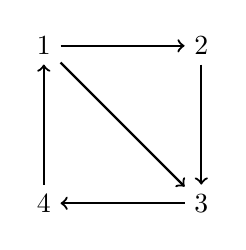
\begin{tikzpicture}
\node (atom1) at (0,2) {$1$};
\node (atom2) at (2,2) {$2$};
\node (atom3) at (2,0) {$3$};
\node (atom4) at (0,0) {$4$};
\draw[->, thick] (atom1)--(atom2);
\draw[->, thick] (atom2)--(atom3);
\draw[->, thick] (atom3)--(atom4);
\draw[->, thick] (atom4)--(atom1);
\draw[->, thick] (atom1) -- (atom3);
\end{tikzpicture}
\bmlDescription{数字 1, 2, 3, 4 由箭头连接。有从 1 指向 2 和 3 的箭头，从 2 指向 3，从 3 指向 4，以及从 4 指向 1 的箭头。}
\end{center}

这个图表可以用来描述一个解释，其论域是前四个正整数，并将“$\atom{R}{x,y}$”解释为仅对以下有序对为真：
\begin{center}
    \ntuple{$1$, $2$},
    \ntuple{$2$, $3$},
    \ntuple{$3$, $4$},
    \ntuple{$4$, $1$},
    \ntuple{$1$, $3$}
\end{center}

同样地，我们也可以给出这个图表：

\begin{center}
\begin{arialabel}{数字 1, 3, 4 由箭头连接。有从 1 指向 3 和自身的箭头，以及从 3 指向 1, 4 和自身的箭头。数字 2 包含在内，但没有箭头进入或指向它。}
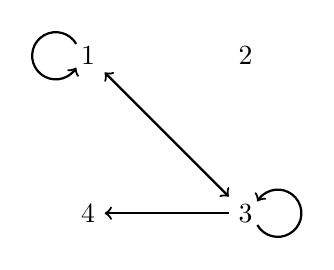
\begin{tikzpicture}
\node (atom1) at (0,2) {$1$};
\node (atom2) at (2,2) {$2$};
\node (atom3) at (2,0) {$3$};
\node (atom4) at (0,0) {$4$};
\draw[->, thick] (atom3)--(atom4);
\draw[->, thick] (atom1)+(-0.15,0.15) arc (-330:-30:.3);
\draw[->, thick] (atom3)+(0.15,-0.15) arc (-150:150:.3);
\draw[<->, thick] (atom1) -- (atom3);
\end{tikzpicture}
\end{arialabel}
\end{center}

由这个图表规定的解释也可以通过列出论域中的元素以及“$\atom{R}{x,y}$”的外延来给出：
\begin{ekey}
    \item[\text{domain}] $1$, $2$, $3$, $4$
    \item[R(x,y)] \ntuple{$1$, $3$},
        \ntuple{$3$, $1$},
        \ntuple{$3$, $4$},
        \ntuple{$1$, $1$},
        \ntuple{$3$, $3$}
\end{ekey}

如果我们愿意，可以让图表更复杂。例如，我们可以添加名称作为特定对象的标签。同样地，为了表示一元谓词的外延，我们可以简单地在某些特定对象周围画一个圈，并规定这些被圈起来的对象（且只有它们）才满足谓词“$\atom{H}{x}$”。为了规定多个谓词，我们可以使用彩色（或虚线、点线）的箭头和圆圈。

\chapter{一阶逻辑中的真}\label{s:TruthFOL}
我们已经介绍了解释。由于解释（除了其他功能外）告诉我们哪些谓词对哪些对象为真，它们将为我们提供原子语句真值的说明。然而，我们现在需要精确地说明，对于一个任意的一阶逻辑语句，在一个解释中为真或为假究竟是什么意思。

我们从\cref{s:FOLSentences}知道，一阶逻辑中有三种类型的语句：
\begin{compactlist}
    \item 原子语句，
    \item 主逻辑算子是语句联结词的语句，
    \item 主逻辑算子是量词的语句。
\end{compactlist}

我们需要为所有这三种类型的语句解释真值。
我们将在本节给出完全一般的解释。不过，为了尽量让解释容易理解，我们会在几个地方使用下面这个解释作为示例：

\begin{ekey}
    \item[\text{domain}] 所有公元2000年以前出生的人
    \item[a] 亚里士多德
    \item[b] 碧昂斯
    \item[\atom{P}{x}] \gap{x} 是哲学家
    \item[\atom{R}{x,y}] \gap{x} 生于 \gap{y} 之前
\end{ekey}

这将是下文\emph{常用的示例}。

\section{原子语句}
原子语句的真值应该是相当直接的。对于语句字母，解释直接规定其为真或为假。语句“$\atom{P}{a}$”为真当且仅当“$\atom{P}{x}$”对“$a$”为真。根据我们的常用示例，这也就是说当且仅当亚里士多德是哲学家。亚里士多德是哲学家，所以该语句为真。同样地，“$\atom{P}{b}$”在我们的常用解释下为假。

类似地，在此解释下，“$\atom{R}{a,b}$”为真当且仅当由“$a$”命名的对象出生于由“$b$”命名的对象之前。亚里士多德确实出生于碧昂斯之前，所以“$\atom{R}{a,b}$”为真。同样地，“$\atom{R}{a,a}$”为假：亚里士多德并非出生于他自己之前。

因此，处理原子语句是非常直观的。当 \metav{R} 是一个 $n$ 元谓词，并且 $\metav{a}_1$、$\metav{a}_{2}$、……、$\metav{a}_{n}$ 是名称时，
\factoidbox{
    语句 $\atom{\metav{R}}{\metav{a}_{1},\metav{a}_{2},\dots,\metav{a}_{n}}$ 在一个解释中为真 \textbf{\ifeff}
    在该解释下，$\metav{R}$ 对由 $\metav{a}_{1}$、$\metav{a}_{2}$、……、$\metav{a}_{n}$（按此顺序）命名的那些对象为真。
}
不过要记住，还有一类特殊的原子语句：由等号连接的两个名称也构成原子语句。这类原子语句同样容易处理。若 \metav{a} 和 \metav{b} 是任意名称，
\factoidbox{
    $\metav{a} = \metav{b}$ 在一个解释中为真 \textbf{\ifeff}
    在该解释下，\metav{a} 和 \metav{b} 命名了完全相同的对象。
}
因此，在我们的常用解释中，“$a = b$”为假，因为亚里士多德和碧昂斯是不同的个体。

\section{句子联结词}
我们在\cref{s:FOLSentences}中看到，一阶逻辑的语句可以用真值函项逻辑中熟悉的真值函项联结词，从更简单的语句构造出来。支配这些真值函项联结词的规则，与我们在真值函项逻辑中所考虑的\emph{完全一样}。它们如下：
\factoidbox{
\begin{factoiditems}
    \item $\metav{A} \eand \metav{B}$ 在一个解释中为真 \textbf{\ifeff} 在该解释下 $\metav{A}$ 与 $\metav{B}$ 均为真。
    \item $\metav{A} \eor \metav{B}$ 在一个解释中为真 \textbf{\ifeff} 在该解释下 $\metav{A}$ 与 $\metav{B}$ 至少有一为真。
    \item $\enot \metav{A}$ 在一个解释中为真 \textbf{\ifeff} 在该解释下 $\metav{A}$ 为假。
    \item $\metav{A} \eif \metav{B}$ 在一个解释中为真 \textbf{\ifeff} 在该解释下 $\metav{A}$ 为假或 $\metav{B}$ 为真。
    \item $\metav{A} \eiff \metav{B}$ 在一个解释中为真 \textbf{\ifeff} 在该解释下 $\metav{A}$ 与 $\metav{B}$ 具有相同的真值。
\end{factoiditems}
}
这与联结词的特征真值表所呈现的信息完全相同，只是呈现方式略有不同。举一些例子或许有助于说明这个想法。（请确保你理解了它们！）在我们的常用解释下：
\begin{itemize}
    \item “$a = a \eand \atom{P}{a}$” 为真。
    \item “$\atom{R}{a,b} \eand \atom{P}{b}$” 为假，因为尽管“$\atom{R}{a,b}$”为真，但“$\atom{P}{b}$”为假。
    \item “$a = b \eor \atom{P}{a}$” 为真。
    \item “$\enot a = b$” 为真。
    \item “$\atom{P}{a} \eand \enot( a= b \eand \atom{R}{a,b})$” 为真，因为“$\atom{P}{a}$”为真而“$a = b$”为假。
\end{itemize}
请确保你理解了这些例子。

\ifHTMLtarget
\section{当主逻辑算子是量词时}
\else
\section[Quantifiers]{当主逻辑算子是量词时}
\fi
\label{s:MainLogicalOperatorQuantifier}

不过，一阶逻辑中令人兴奋的创新在于\emph{量词}的使用，但为量化语句表述真值条件，却比最初想象的更繁琐一些。

这里有一个朴素的最初想法。我们想说“$\forall x\, \atom{F}{x}$”为真当且仅当“$\atom{F}{x}$”对论域中的每一个对象为真。这应该问题不大：我们的解释会直接规定“$\atom{F}{x}$”对哪些对象为真。

不幸的是，这个朴素的想法不够普遍。例如，我们希望能够在（粗略来说）“$\exists y\, \atom{L}{x,y}$” 对论域中每一对象都为真的情况下，断定 “$\forall x \exists y\, \atom{L}{x,y}$” 为真。但我们的解释并\emph{没有直接}规定 “$\exists y\, \atom{L}{x,y}$” 对什么为真。相反，该公式是否对某物为真，应当仅从谓词 “$L$” 的解释、论域以及量词的含义中得出。

因此，我们转向第二个朴素想法。我们可以尝试说，“$\forall x \exists y\, \atom{L}{x,y}$” 在一个解释中为真 \ifeff{} 对我们解释中所包含的\emph{每一个}名称 \metav{a} 而言，$\exists y\, \atom{L}{\metav{a},y}$ 都为真。类似地，我们可以尝试说，$\exists y\, \atom{L}{\metav{a},y}$ 为真当且仅当对我们解释中所包含的\emph{某个}名称 \metav{b} 而言，$\atom{L}{\metav{a},\metav{b}}$ 为真。

不幸的是，这同样不对。为了看清这一点，注意到我们的默认解释只解释了\emph{两个}名称，即 “$a$” 和 “$b$”。但论域（所有公元2000年之前出生的人）所包含的人远多于两个。（而且我们也无意通过命名\emph{所有人}来修正这一点！）

于是我们有了第三种想法。（这次的想法并非朴素，而是正确的。）尽管我们并没有给\emph{每个人}命名，但每个人\emph{都可能}被赋予一个名称。因此，我们应该专注于通过添加一个新名称来扩展解释的可能性。我们将以我们的默认解释为中心，举几个这方面的例子，然后再提出正式定义。

在我们的默认解释中，“$\exists x\, \atom{R}{b,x}$” 应为真。毕竟，在该论域中，确实有人出生在 Beyonc\'e 之后。Lady Gaga 便是其中之一。事实上，如果我们（请注意，这只是临时的）通过添加新名称 “$c$” 来指称 Lady Gaga 以扩展默认解释，那么在此扩展解释上 “$\atom{R}{b,c}$” 将为真。这无疑应足以使得 “$\exists x\, \atom{R}{b,x}$” 在原始默认解释上为真。

在我们的默认解释中，“$\exists x (\atom{P}{x} \eand \atom{R}{x,a})$” 也应为真。毕竟，在该论域中，确实有人既是哲学家又生于亚里士多德之前。苏格拉底就是这样一个人。事实上，如果我们通过让一个新名称 “$c$” 指称苏格拉底来扩展默认解释，那么在此扩展解释上 “$\atom{P}{c} \eand \atom{R}{c,a}$” 将为真。同样，这无疑应足以使得 “$\exists x (\atom{P}{x} \eand \atom{R}{x,a})$” 在原始默认解释上为真。

在我们的默认解释中，“$\forall x \exists y\, \atom{R}{x,y}$” 应为假。毕竟，考虑1999年出生的最后一个人。我们不知道此人是谁，但如果我们通过让一个新名称 “$d$” 指称此人来扩展默认解释，那么我们将无法在论域中找到另一个人并用某个进一步的新名称（例如 “$e$”）去指称，使得 “$\atom{R}{d,e}$” 为真。的确，无论我们用 “$e$” 命名\emph{谁}，“$\atom{R}{d,e}$” 都将为假。这一观察无疑足以使 “$\exists y\, \atom{R}{d,y}$” 在我们扩展的解释中为\emph{假}，而这又无疑足以使 “$\forall x \exists y\, \atom{R}{x,y}$” 在原始默认解释上为假。

如果你理解了这三个例子，那便掌握了要义。这为量化语句的真值定义奠定了基础。

然而，严格来说，我们仍需\emph{给出}那个定义。遗憾的是，结果有些繁琐，且需要引入几个新定义。请做好准备！

假设 \metav{A} 是一个公式。我们将用 $$\metav{A}(\ldots \metav{x} \ldots \metav{x} \ldots)$$ 来表示 \metav{A} 包含若干（通常是一个或多个，但我们也不排除 \metav{x} 根本没有自由出现的情况）变元~\metav{x} 的自由出现。同时假设 \metav{c} 是一个名称。那么，我们将用：
$$\metav{A}(\ldots \metav{c} \ldots \metav{c} \ldots)$$
表示将 \metav{A} 中 $\metav{x}$ 的\emph{每一个}自由出现替换为~$\metav{c}$ 后得到的公式。所得公式称为 $\forall \metav{x}\metav{A}$ 与 $\exists\metav{x}\metav{A}$ 的一个 \define{代入实例}。同时，$\metav{c}$ 被称为 \define{实例化名称}。（如果 \metav{A} 碰巧不含~\metav{x} 的自由出现，则该代入实例就与~\metav{A} 相同。例如，
	$$\exists x (\atom{R}{e,x} \eiff \atom{F}{x})$$
就是
	$$\forall y \exists x (\atom{R}{y,x} \eiff \atom{F}{x})$$
的一个代入实例，其实例化名称是 “$e$”，被实例化的变元是~“$y$”。）

\newglossaryentry{substitution instance}{
  name = 代入实例,
  description = {将一个\gls{formula}中某个\gls{variable}的所有自由出现替换为一个\gls{name}后得到的结果}
}

顺带一提：在用名称替换变元时，我们只允许替换\emph{自由}变元。这是必要的，因为我们允许像 “$\exists x(\forall x\,\atom{F}{x} \eif
\atom{G}{x})$' 这样的公式，其中不同的量词可以约束相同的变元。我们仅将 “$\forall x\,\atom{F}{x} \eif \atom{G}{e}$” 视作该公式的代入实例，而不将 “$\atom{F}{e} \eif
\atom{G}{e}$' 视作代入实例，因为 “$\atom{F}{x}$” 中的 “$x$” 并非自由变元——它被 “$\forall x$” 所约束。（关于这一点，你可能需要回顾 \cref{s:FreeVars}。）

我们的解释会规定哪些名称对应论域中的哪些对象。取论域中任意对象，记为 d，并取一个解释尚未指派的名称 $\metav{c}$。如果我们的解释是 $\mathbf{I}$，则可考虑解释 $\mathbf{I}[\text{d}/\metav{c}]$，它与 $\mathbf{I}$ 完全相同，只是\emph{额外}将对象~d 指派给名称 $\metav{c}$。那么，我们便可以说，对象 d 在解释~$\mathbf{I}$ 下 \define{满足} 公式 $\metav{A}(\dots\metav{x}\dots\metav{x}\dots)$，当且仅当 $\metav{A}(\dots\metav{c}\dots\metav{c}\dots)$ 在 $\mathbf{I}[\text{d}/\metav{c}]$ 下为真。（我们假设名称 $\metav{c}$ 尚未在 $\metav{A}(\dots\metav{x}\dots\metav{x}\dots)$ 中出现。）若 d 满足 $\metav{A}(\dots\metav{x}\dots\metav{x}\dots)$，我们也称 $\metav{A}(\dots\metav{x}\dots\metav{x}\dots)$ \emph{对} d 成立。

\factoidbox{

\begin{factoiditems}
		\item 解释 $\mathbf{I}[\text{d}/\metav{c}]$ 与解释 $\mathbf{I}$ 完全相同，只是额外将对象~d 指派给名称 $\metav{c}$。
		\item 对象 d 在解释~$\mathbf{I}$ 下 \define{满足} $\metav{A}(\dots\metav{x}\dots\metav{x}\dots)$，\textbf{\ifeff} $\metav{A}(\dots\metav{c}\dots\metav{c}\dots)$ 在 $\mathbf{I}[\text{d}/\metav{c}]$ 下为真（其中名称 $\metav{c}$ 未在 $\metav{A}(\dots\metav{x}\dots\metav{x}\dots)$ 中出现过）。
	\end{factoiditems}

}

\newglossaryentry{satisfaction}
{
  name=公式的满足,
  description={指论域中的对象 d 与解释~$\mathbf{I}$ 下的 \gls{formula}~$\metav{A}(\metav{x})$ 之间的一种关系，该关系成立 \ifeff{} $\metav{A}(\metav{c})$ 在修改后的解释 $\mathbf{I}[\text{d}/\metav{c}]$ 中为真，其中 $\metav{c}$ 命名了~d}
}

例如，苏格拉底满足公式~$\atom{P}{x}$，因为 $\atom{P}{c}$ 在解释 $\mathbf{I}[\text{Socrates}/c]$ 下为真，即下面的解释：

\begin{ekey}
	\item[\text{domain}] 所有公元2000年以前出生的人
	\item[a] 亚里士多德
	\item[b] 碧昂丝
	\item[c] 苏格拉底
	\item[\atom{P}{x}] \gap{x} 是哲学家
	\item[\atom{R}{x,y}] \gap{x} 出生在 \gap{y} 之前
\end{ekey}

借助这一记法，大致思路如下。句子 $\forall \metav{x}\metav{A}(\ldots \metav{x} \ldots \metav{x} \ldots)$ 在 $\mathbf{I}$ 下为真 \ifeff{} 对于论域中的每个对象~d，$\metav{A}(\ldots \metav{c} \ldots \metav{c}\ldots)$ 在 $\mathbf{I}[\text{d}/\metav{c}]$ 下为真，即，无论我们用新名称~$\metav{c}$ 来指称论域中的哪个对象。换句话说，$\forall \metav{x} \metav{A}(\ldots \metav{x} \ldots \metav{x}
\ldots)$ 为真 \ifeff{} 论域中每个对象都满足 $\metav{A}(\ldots \metav{x} \ldots \metav{x} \ldots)$。类似地，句子 $\exists \metav{x}\metav{A}(\ldots \metav{x} \ldots \metav{x}
\ldots)$ 在 $\mathbf{I}$ 下为真 \ifeff{} 存在\emph{某个}对象满足 $\metav{A}(\ldots \metav{x} \ldots \metav{x}
\ldots)$，即，对于某个对象~d 和某个新名称~$\metav{c}$，$\metav{A}(\ldots \metav{c} \ldots \metav{c} \ldots)$ 在 $\mathbf{I}[\text{d}/\metav{c}]$ 下为真。
\factoidbox{

\begin{factoiditems}
		\item $\forall \metav{x}\metav{A}(\ldots \metav{x}\ldots\metav{x}\ldots)$ 在一个解释下为真 \textbf{\ifeff} 论域中每个对象都满足 $\metav{A}(\ldots
		\metav{x} \ldots \metav{x}\ldots)$。
		\item $\exists \metav{x}\metav{A}(\ldots \metav{x}\ldots\metav{x}\ldots)$ 在一个解释下为真 \textbf{\ifeff} 论域中至少有一个对象满足 $\metav{A}(\ldots \metav{x}\ldots\metav{x}\ldots)$。
		\end{factoiditems}

	}
需要明确的是：所有这些工作只是（以一种非常迂腐的方式）将上面阐述的直观想法形式化。结果有些繁琐，最终的定义可能略显晦涩。但希望其\emph{核心思想}是清晰的。

\practiceproblems
\solutions
\problempart
\label{pr.TorF1}
考虑以下解释：

\begin{itemize}
		\item 论域仅包含 Corwin 和 Benedict
		\item “$\atom{A}{x}$” 对 Corwin 和 Benedict 都为真
		\item “$\atom{B}{x}$” 仅对 Benedict 为真
		\item “$\atom{N}{x}$” 不对任何人为真
		\item “$c$” 指称 Corwin
	\end{itemize}

判断以下每个句子在该解释下是真还是假：

\begin{compactlist}
\item $\atom{B}{c} $
\item $\atom{A}{c}  \eiff \enot \atom{N}{c}$
\item $\atom{N}{c}  \eif (\atom{A}{c} \eor \atom{B}{c})$
\item $\forall x\, \atom{A}{x}$
\item $\forall x \enot \atom{B}{x}$
\item $\exists x(\atom{A}{x} \eand \atom{B}{x})$
\item $\exists x(\atom{A}{x} \eif \atom{N}{x})$
\item $\forall x(\atom{N}{x} \eor \enot \atom{N}{x})$
\item $\exists x\, \atom{B}{x} \eif \forall x\, \atom{A}{x}$
\end{compactlist}

\problempart
\label{pr.TorF2}
考虑以下解释：

\begin{itemize}
		\item 论域仅包含 Lemmy, Courtney 和 Eddy
		\item “$\atom{G}{x}$” 对 Lemmy, Courtney 和 Eddy 都为真。
		\item “$\atom{H}{x}$” 仅对 Courtney 为真
		\item “$\atom{M}{x}$” 仅对 Lemmy 和 Eddy 为真
		\item “$c$” 指称 Courtney
		\item “$e$” 指称 Eddy
	\end{itemize}

判断以下每个句子在该解释下是真还是假：

\begin{compactlist}
\item $\atom{H}{c} $
\item $\atom{H}{e} $
\item $\atom{M}{c}  \eor \atom{M}{e}$
\item $\atom{G}{c}  \eor \enot \atom{G}{c}$
\item $\atom{M}{c}  \eif \atom{G}{c}$
\item $\exists x\, \atom{H}{x}$
\item $\forall x\, \atom{H}{x}$
\item $\exists x\, \enot \atom{M}{x}$
\item $\exists x(\atom{H}{x} \eand \atom{G}{x})$
\item $\exists x(\atom{M}{x} \eand \atom{G}{x})$
\item $\forall x(\atom{H}{x} \eor \atom{M}{x})$
\item $\exists x\, \atom{H}{x} \eand \exists x\, \atom{M}{x}$
\item $\forall x(\atom{H}{x} \eiff \enot \atom{M}{x})$
\item $\exists x\, \atom{G}{x} \eand \exists x \enot \atom{G}{x}$
\item $\forall x\exists y(\atom{G}{x} \eand \atom{H}{y})$
\end{compactlist}

\problempart
\label{pr.TorF3}
遵循在\cref{s:Interpretations}末尾引入的图示惯例，考虑以下解释：


\begin{center}
\begin{arialabel}{数字 1、2、3、4、5 由箭头连接。存在从 1 到 2、3、4、5 以及到自身的箭头，从 2 到 5 的箭头，从 5 到自身的箭头，以及从 4 到 1 的箭头。3 没有箭头射出。}
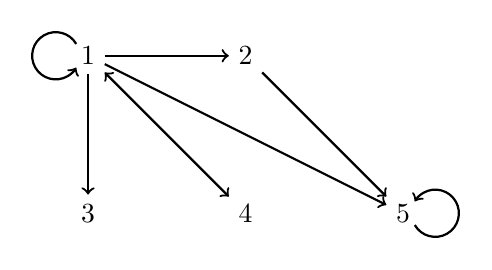
\begin{tikzpicture}
\node (atom1) at (0,2) {$1$};
\node (atom2) at (2,2) {$2$};
\node (atom4) at (0,0) {$3$};
\node (atom5) at (2,0) {$4$};
\node (atom6) at (4,0) {$5$};
\draw[->, thick] (atom1)+(-0.15,0.15) arc (-330:-30:.3);
\draw[->, thick] (atom6)+(0.15,-0.15) arc (-150:150:.3);
\draw[->, thick] (atom1) -- (atom2);
\draw[->, thick] (atom1) -- (atom4);
\draw[<->, thick] (atom1) -- (atom5);
\draw[->, thick] (atom1) -- (atom6);
\draw[->, thick] (atom2) -- (atom6);
\end{tikzpicture}
\end{arialabel}
\end{center}


确定以下每个句子在该解释下是真的还是假的：


\begin{compactlist}
\item $\exists x\, \atom{R}{x,x}$
\item $\forall x\, \atom{R}{x,x}$
\item $\exists x \forall y\, \atom{R}{x,y}$
\item $\exists x \forall y\, \atom{R}{y,x}$
\item $\forall x \forall y \forall z ((\atom{R}{x,y} \eand \atom{R}{y,z}) \eif \atom{R}{x,z})$
\item $\forall x \forall y \forall z ((\atom{R}{x,y} \eand \atom{R}{x,z}) \eif \atom{R}{y,z})$
\item $\exists x \forall y\, \enot \atom{R}{x,y}$
\item $\forall x(\exists y\, \atom{R}{x,y} \eif \exists y\, \atom{R}{y,x})$
\item $\exists x \exists y (\enot x = y \eand \atom{R}{x,y} \eand \atom{R}{y,x})$
\item $\exists x \forall y(\atom{R}{x,y} \eiff x = y)$
\item $\exists x \forall y(\atom{R}{y,x} \eiff x = y)$
\item $\exists x \exists y(\enot x = y \eand \atom{R}{x,y} \eand \forall z(\atom{R}{z,x} \eiff y = z))$
\end{compactlist}

\chapter{语义概念}

\section{有效性、蕴涵等}

在一阶逻辑中定义真相当繁琐。但现在既然已经完成，我们就可以定义其他各种核心逻辑概念。这些定义看起来与真值函项逻辑中的定义非常相似（参见\cref{s:SemanticConcepts}）。然而，请记住这里涉及的是\emph{解释}，而非赋值。

我们将像在真值函项逻辑中那样，在一阶逻辑中也使用符号“$\entails$”。因此，
语句 $\metav{A}_1, \metav{A}_2, \ldots, \metav{A}_n$
\define{蕴涵}语句 $\metav{C}$，
	$$\metav{A}_1, \metav{A}_2, \ldots, \metav{A}_n \entails\metav{C},$$
\ifeff{} 不存在一个解释，在其中所有 $\metav{A}_1$, $\metav{A}_2$, \dots, $\metav{A}_n$ 都为真而 $\metav{C}$ 为假。由此可得，
	$$\entails\metav{A}$$
意味着 $\metav{A}$ 在每一个解释中均为真。

其他逻辑概念在一阶逻辑中也有相应的定义：

\factoidbox{


\begin{factoiditems}
		\item 一个一阶逻辑语句 $\metav{A}$ 是\define{有效式} \ifeff{}
		$\metav{A}$ 在每一个解释中均为真；即 $\entails\metav{A}$。
\newglossaryentry{validity}
{
name=逻辑有效式,
description={一个在每一个\gls{interpretation}下都为真的\gls{sentence of FOL}}
}

		\item $\metav{A}$ 是\define{矛盾式} \ifeff{} $\metav{A}$
		在每一个解释中均为假；即 $\entails\enot\metav{A}$。
\newglossaryentry{contradiction of FOL}
{
  name=矛盾式（一阶逻辑）,
  text=矛盾式,
description={一个在每一个\gls{interpretation}下都为假的\gls{sentence of FOL}}
}

		\item $\metav{A}_1, \metav{A}_2, \ldots, \metav{A}_n \therefore
		\metav{C}$ 是\define{有效的（于一阶逻辑中）} \ifeff{} 不存在一个解释，使得所有前提为真且结论为假；即 $\metav{A}_1,\metav{A}_2,\ldots,
		\metav{A}_n \entails\metav{C}$。否则它是\define{无效的（于一阶逻辑中）}。
\newglossaryentry{valid in FOL}
{
  name=论证的有效性（一阶逻辑）,
  text = 有效,
description={论证所具有的性质；一个论证是有效的当且仅当没有\gls{interpretation}能使所有前提为真而结论为假}
}

		\item 两个一阶逻辑语句 \metav{A} 和 \metav{B} 是\define{等值的} \ifeff{} 它们在完全相同的解释中彼此同为真；即同时有
		$\metav{A}\entails\metav{B}$ 和 $\metav{B}\entails\metav{A}$。

\newglossaryentry{equivalent in FOL}
{
  name=等值性（一阶逻辑）,
  text = 等值,
description={成对的\glspl{sentence of FOL}所具有的性质，当且仅当这些句子在每一个\gls{interpretation}下都有相同的真值}
}

		\item 一阶逻辑语句 $\metav{A}_1$, $\metav{A}_2$, \dots,
		$\metav{A}_n$ 是\define{共同可满足的} \ifeff{} 存在某个解释使它们全部为真。它们是\define{共同不可满足的} \ifeff{} 不存在这样的解释。
\newglossaryentry{satisfiable in FOL}
{
  name=可满足性（一阶逻辑）,
  text=共同可满足,
  description={\glspl{sentence of FOL}所具有的性质，当且仅
  当存在某个\gls{interpretation}能使所有这些句子同时为真}
}
	\end{factoiditems}


}

注意，我们使用“有效式”这一标准术语来指称在每一解释下都为真的句子。有效式之于一阶逻辑，就如同重言式之于真值函项逻辑。

\section{表达力}

在\cref{s:MainLogicalOperatorQuantifier}中引入的“对象满足含一个自由变元的公式”这一概念，也可以扩展到含多个自由变元的公式。如果我们有一个
公式 $\metav{A}(\metav{x},\metav{y})$ 带有两个自由变元 $\metav{x}$ 和 $\metav{y}$，那么我们可以说一个对象对 $\langle a, b\rangle$ 满足 $\metav{A}(\metav{x},\metav{y})$
\ifeff{} $\metav{A}(\metav{c},\metav{d})$ 在通过添加两个名称 $\metav{c}$ 和 $\metav{d}$ 而扩展的解释中为真，其中 $\metav{c}$ 指称~$a$ 而 $\metav{d}$ 指称~$b$。举例来说，$\langle \text{Socrates}, \text{Plato}\rangle$ 满足
$\atom{R}{x,y}$，因为在这个解释中 $\atom{R}{c,d}$ 为真：

\begin{ekey}
	\item[\text{domain}] 公元2000年前出生的所有人
	\item[a] Aristotle
	\item[b] Beyonc\'e
	\item[c] Socrates
	\item[d] Plato
	\item[\atom{P}{x}] \gap{x} 是哲学家
	\item[\atom{R}{x,y}] \gap{x} 出生于 \gap{y} 之前
\end{ekey}

对于原子公式，满足它们的对象、对象对等，正是解释中给出的谓词的外延。但“满足”这一概念也适用于非原子公式，例如，公式 $\atom{P}{x} \land \atom{R}{x,b}$ 被所有在 Beyonc\'e 之前出生的哲学家所满足。它甚至适用于包含量词的公式，例如，$\atom{P}{x} \eand \lnot\exists y(\atom{P}{y} \land \atom{R}{y,x})$ 被所有本身是哲学家且没有别的哲学家出生于他们之前的人所满足——换句话说，该公式对于第一位哲学家为真。

通过考虑带有两个自由变元的公式（可能包含量词），我们可以表达那些在我们的解释或符号化约定中没有专门谓词符号的关系。考虑公式 $\atom{R}{x,y}$。它表达了“\gap{x} 出生于 \gap{y} 之前”这一关系，因为我们正是这样规定其外延的。如果我们交换变元，也就是考虑“$\atom{R}{y,x}$”，会发生什么？论域中的一个对象对 \ntuple{$\text{y}, \text{x}$}（即一对人）满足 $\atom{R}{y,x}$ 当且仅当，反过来的一对 \ntuple{$\text{x}, \text{y}$} 满足 $\atom{R}{x,y}$。换句话说，$\atom{R}{y,x}$ 表达的是“\gap{x} 出生于 \gap{y} \emph{之后}”这一关系。或者假设我们在解释中添加一个表示“……是……的老师”的谓词。


\begin{ekey}
	\item[\atom{T}{x,y}] \gap{x} 是 \gap{y} 的老师
\end{ekey}


那么公式“$\exists z(\atom{T}{z,x} \land \atom{T}{z,y})$”被 x 和 y 满足当且仅当，存在某个人 z 既是 x 的老师也是 y 的老师，也就是说，它表达了“\gap{x} 和 \gap{y} 有共同的老师”。类似地，“$\forall z(\atom{T}{x,z} \eiff \atom{T}{y,
z})$”表达了“\gap{x} 和 \gap{y} 教的是同一批人”。

这些例子的要旨是，有些英语谓词，比如“\gap{x} 和 \gap{y} 有共同的老师”，有时即使没有现成的明确谓词符号，也可以在解释中表达出来。如果是这种情况，你可以使用一个表达该谓词的公式（比如“$\exists
z(\atom{T}{z,x} \land \atom{T}{z,y})$”）来符号化涉及该谓词的英语句子。

\practiceproblems

\problempart
给定以下解释：


\begin{ekey}
	\item[\text{domain}] 所有人
	\item[\atom{W}{x}] \gap{x} 是女性（或女孩）
	\item[\atom{M}{x}] \gap{x} 是男性（或男孩）
	\item[\atom{Y}{x,y}] \gap{x} 比 \gap{y} 年轻
	\item[\atom{O}{x,y}] \gap{x} 是 \gap{y} 的后代
	\item[d] Dana
	\item[a] Alex
\end{ekey}


用公式表达以下关系：


\begin{compactlist}
	\item \gap{x} 比 \gap{y} 年长
	\item \gap{x} 是 \gap{y} 的母亲
	\item \gap{x} 和 \gap{y} 是兄弟姐妹（注意：自己不能是自己的兄弟姐妹）
	\item \gap{x} 是 \gap{y} 的兄弟
\end{compactlist}

\problempart
使用上一练习中的符号化约定，将以下句子符号化：


\begin{compactlist}
	\item Alex 和 Dana 是姐妹。
	\item 父亲都比他们的孩子年长。
	\item Alex 的父母年龄相同。
\end{compactlist}

\chapter{使用解释}
\label{sec.UsingModels}

\section{有效式与矛盾式}
假设我们想证明“$\exists x\, \atom{A}{x,x} \eif \atom{B}{d}$”\emph{不是}一个有效式。这需要证明该语句并非在每个解释中都为真；也就是说，它在某个解释中为假。如果我们能提供一个该语句在其中为假的解释，那么就证明了该语句不是有效式。

要使“$\exists x\,\atom{A}{x,x} \eif \atom{B}{d}$”为假，其前件（“$\exists x\, \atom{A}{x,x}$”）必须为真，而后件（“$\atom{B}{d}$”）必须为假。为了构造这样的解释，我们首先规定一个论域。论域小一些可以更容易规定谓词对哪些对象为真，所以我们从一个只有一个成员的论域开始。为了具体起见，我们就说它\emph{仅仅}是巴黎这座城市。


\begin{ekey}
		\item[\text{domain}] 巴黎
	\end{ekey}


名称“$d$”必须指称论域中的某个东西，所以我们别无选择：


\begin{ekey}
		\item[d] 巴黎
	\end{ekey}


回想一下，我们希望“$\exists x\, \atom{A}{x,x}$”为真，所以我们希望论域中的所有成员都在谓词“$A$”的外延中与自身配对。我们可以简单地给出：


\begin{ekey}
		\item[\atom{A}{x,y}] \gap{x} 与 \gap{y} 是同一个东西
	\end{ekey}


现在“$\atom{A}{d,d}$”为真，所以“$\exists x\, \atom{A}{x,x}$”当然为真。接着，我们希望“$\atom{B}{d}$”为假，所以“$d$”的所指不能在“$B$”的外延中。我们可以简单地给出：


\begin{ekey}
		\item[\atom{B}{x}] \gap{x} 在德国
	\end{ekey}

现在我们有了一个解释，使得 “$\exists x\, \atom{A}{x,x}$” 为真，但 “$\atom{B}{d}$” 为假。所以存在一个解释使得 “$\exists x\, \atom{A}{x,x} \eif \atom{B}{d}$” 为假。因此，“$\exists x\, \atom{A}{x,x} \eif \atom{B}{d}$” 不是有效式。

我们可以同样轻易地证明 “$\exists x\,\atom{A}{x,x} \eif \atom{B}{d}$” 不是矛盾式。我们只需给出一个使 “$\exists x\,\atom{A}{x,x} \eif \atom{B}{d}$” 为真的解释；也就是说，一个使 “$\exists x\, \atom{A}{x,x}$” 为假或 “$\atom{B}{d}$” 为真的解释。例如：


\begin{ekey}
		\item[\text{domain}] Paris
		\item[d] Paris
		\item[\atom{A}{x,y}] \gap{x} 与 \gap{y} 相同
		\item[\atom{B}{x}] \gap{x} 在法国
	\end{ekey}


这表明存在一个解释使得 “$\exists x\,\atom{A}{x,x} \eif \atom{B}{d}$” 为真。所以 “$\exists x\, \atom{A}{x,x} \eif \atom{B}{d}$” 不是矛盾式。
	\factoidbox{


\begin{factoiditems}
			\item 要证明 $\metav{A}$ 不是有效式，只需找到一个使 $\metav{A}$ 为假的解释。
			\item 要证明 $\metav{A}$ 不是矛盾式，只需找到一个使 $\metav{A}$ 为真的解释。
		\end{factoiditems}


	}

\section{逻辑等价}
假设我们想证明 “$\forall x\, \atom{S}{x}$” 和 “$\exists x\, \atom{S}{x}$” 不是逻辑等价的。我们需要构造一个解释，使得这两个语句具有不同的真值；我们需要其中一个为真，另一个为假。我们从指定一个论域开始。同样，我们让论域小一些，以便轻松指定外延。在这种情况下，我们至少需要两个对象。（如果我们选择只有一个成员的论域，这两个语句最终会具有相同的真值。要想知道原因，可以尝试构造一些只有一个成员的论域的部分解释。）为具体起见，我们取：


\begin{ekey}
		\item[\text{domain}] Ornette Coleman, Miles Davis
	\end{ekey}


我们可以通过将某些东西放入 “$S$” 的外延中，使 “$\exists x\, \atom{S}{x}$” 为真；也可以通过将某些东西排除在 “$S$” 的外延之外，使 “$\forall x\, \atom{S}{x}$” 为假。为具体起见，我们规定：


\begin{ekey}
		\item[\atom{S}{x}] \gap{x} 演奏萨克斯风
	\end{ekey}


现在 “$\exists x\, \atom{S}{x}$” 为真，因为 “$\atom{S}{x}$” 对于 Ornette Coleman 成立。更准确一点说，通过允许 “$c$” 指称 Ornette Coleman 来扩展我们的解释。在这个扩展的解释中，“$\atom{S}{c}$” 为真，因此在原始的解释中 “$\exists x\, \atom{S}{x}$” 为真。类似地，“$\forall x\, \atom{S}{x}$” 为假，因为 “$\atom{S}{x}$” 对于 Miles Davis 不成立。更准确一点说，通过允许 “$d$” 指称 Miles Davis 来扩展我们的解释，在这个扩展的解释中 “$\atom{S}{d}$” 为假，因此在原始的解释中 “$\forall x\, \atom{S}{x}$” 为假。我们为 “$\forall x\, \atom{S}{x}$” 和 “$\exists x\, \atom{S}{x}$” 是逻辑等价的这一主张提供了一个反解释。
	\factoidbox{
		要证明 $\metav{A}$ 和 $\metav{B}$ 不是逻辑等价的，只需找到一个解释使得其中一个为真而另一个为假。
	}

\section{有效性、蕴涵与可满足性}
要测试有效性、蕴涵或可满足性，我们通常需要构造能同时确定多个语句真值的解释。

考虑下面这个一阶逻辑中的论证：
$$\exists x(\atom{G}{x} \eif \atom{G}{a}) \therefore \exists x\, \atom{G}{x} \eif \atom{G}{a}$$
为了证明它是无效的，我们必须使前提为真且结论为假。结论是一个条件句，因此要使其为假，前件必须为真而后件必须为假。显然，我们的论域必须包含两个对象。我们尝试：


\begin{ekey}
		\item[\text{domain}] Karl Marx, Ludwig von Mises
		\item[\atom{G}{x}] \gap{x} 憎恨共产主义
		\item[a] Karl Marx
	\end{ekey}


考虑到马克思撰写了《共产党宣言》，“$\atom{G}{a}$” 在这个解释中显然为假。但米塞斯以憎恨共产主义闻名，因此 “$\exists x\, \atom{G}{x}$” 在这个解释中为真。因此 “$\exists x\, \atom{G}{x} \eif \atom{G}{a}$” 为假，正如所要求的那样。

这个解释使得前提为真吗？是的！注意 “$\atom{G}{a} \eif \atom{G}{a}$” 为真。（事实上，它是一个有效式。）那么 “$\exists x (\atom{G}{x} \eif \atom{G}{a})$” 当然也为真，所以在这个解释中，前提为真而结论为假。因此该论证是无效的。

顺带一提，注意我们也证明了 “$\exists x(\atom{G}{x} \eif \atom{G}{a})$” 并\emph{不}蕴涵 “$\exists x\, \atom{G}{x} \eif \atom{G}{a}$”，即 $\exists x (\atom{G}{x} \eif \atom{G}{a}) \nentails \exists x\, \atom{G}{x} \eif \atom{G}{a}$。同样，我们也证明了语句 “$\exists x (\atom{G}{x} \eif \atom{G}{a})$” 和 “$\enot (\exists x\, \atom{G}{x} \eif \atom{G}{a})$” 是共同可满足的。

我们考虑第二个例子：
$$\forall x \exists y\, \atom{L}{x,y} \therefore \exists y \forall x\, \atom{L}{x,y}$$
同样，我们想要证明它是无效的。为此，我们必须使前提为真而结论为假。以下是一个建议：


\begin{ekey}
	\item[\text{domain}] 目前与另一加拿大公民处于国内伴侣关系中的加拿大公民
	\item[\atom{L}{x,y}] \gap{x} 与 \gap{y} 处于国内伴侣关系中
\end{ekey}

在这一解释下，前提显然为真。论域中的每个人都与某个其他加拿大籍人士存在伴侣关系。那个其他人也会在论域中。因此，对于论域中的每个人，都存在论域中的某个（不同的）人与他处于伴侣关系中。所以 “$\forall x \exists y\, \atom{L}{x,y}$” 为真。然而，结论显然为假，因为这要求存在一个单独的人，他与论域中的每个人都处于伴侣关系中，而并不存在这样的人，所以该论证是无效的。我们立即观察到，语句 “$\forall x \exists y\, \atom{L}{x,y}$” 和 “$\enot\exists y \forall x\, \atom{L}{x,y}$” 是共同可满足的，并且 “$\forall x \exists y\, \atom{L}{x,y}$” 不蕴涵 “$\exists y \forall x\, \atom{L}{x,y}$”。

作为第三个例子，我们来把事情混合一下。在 \cref{s:Interpretations} 中，我们描述了如何使用图示来展现某些解释。例如：

\begin{center}
	\begin{arialabel}{数字1、2和3由箭头连接。有从1指向2、3和它自身的箭头，以及从2指向3的箭头。没有从3指出的箭头。}
	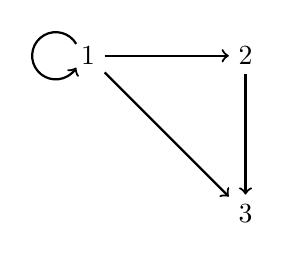
\begin{tikzpicture}
	\node (atom1) at (0,2) {1};
	\node (atom2) at (2,2) {2};
	\node (atom3) at (2,0) {3};
	\draw[->, thick] (atom1)--(atom2);
	\draw[->, thick] (atom1)--(atom3);
	\draw[->, thick] (atom1)+(-0.15,0.15) arc (-330:-30:.3);
	\draw[->, thick] (atom2) -- (atom3);
\end{tikzpicture}
\end{arialabel}
\end{center}

采用 \cref{s:Interpretations} 中使用的约定，这一解释的论域是前三个正整数，并且当且仅当在我们的图中有从 x 指向 y 的箭头时，“$\atom{R}{x,y}$” 对 x 和 y 为真。以下是该解释使其为真的一些语句：

\begin{itemize}
	\item “$\forall x \exists y\, \atom{R}{y,x}$”
	\item “$\exists x \forall y\, \atom{R}{x,y}$” \hfill ($x$ 的见证：$1$)
	\item “$\exists x \forall y (\atom{R}{y,x} \eiff x = y)$” \hfill ($x$ 的见证：$1$)
	\item “$\exists x \exists y \exists z ((\enot y = z \eand \atom{R}{x,y}) \eand \atom{R}{z,x})$” \hfill ($x$ 的见证：$2$)
	\item “$\exists x \forall y\, \enot \atom{R}{x,y}$” \hfill ($x$ 的见证：$3$)
	\item “$\exists x (\exists y\, \atom{R}{y,x} \eand \enot \exists y\, \atom{R}{x,y})$” \hfill ($x$ 的见证：$3$)
\end{itemize}

这立即表明，前面六个语句都是共同可满足的。我们可以利用这一观察来构造\emph{无效}论证，例如：
\begin{align*}
	\forall x \exists y\, \atom{R}{y,x}, \exists x \forall y\, \atom{R}{x,y}  &\therefore  \forall x \exists y\, \atom{R}{x,y}\\
	\exists x \forall y\, \atom{R}{x,y}, \exists x \forall y \enot \atom{R}{x,y} & \therefore \enot \exists x \exists y \exists z (\enot y = z \eand (\atom{R}{x,y} \eand \atom{R}{z,x}))
\end{align*}
以及除此之外的许多其他例子。

\factoidbox{
	如果某个解释使得 $\metav{A}_1, \metav{A}_2, \ldots, \metav{A}_n$ 全部为真而 $\metav{C}$ 为假，那么：


\begin{compactlist}
		\item$\metav{A}_1, \metav{A}_2, \ldots, \metav{A}_n \therefore \metav{C}$ 是\emph{无效的}；并且
	\item $\metav{A}_1, \metav{A}_2, \ldots, \metav{A}_n \nentails \metav{C}$；并且
	\item
	并且 $\metav{A}_1, \metav{A}_2, \ldots, \metav{A}_n, \enot \metav{C}$ 是共同可满足的。
\end{compactlist}
}
能够反驳某个说法（例如对逻辑真理的声称，或对蕴涵的声称）的解释，被称为\emph{反解释（counter-interpretation）}，或称\emph{反模型（counter-model）}。

不过，在结束本节之前，我们要提醒一下（无）有效性与（非）蕴涵之间的关系。回想一下一阶逻辑的局限性：它是一种外延性语言；它忽略了模糊性问题；它无法处理因“特殊原因”而有效的情况。为了展示这些问题中的一个例子，考虑下面这个自然语言论证：

\begin{earg}
	\item[] 每只狐狸都很可爱。
	\item[\texttherefore] 所有雌狐都很可爱。
\end{earg}

这在概念上是有效的：雌狐必然是狐狸，所以前提为真而结论为假是不可能的。那么，我们可以合理地将这个论证符号化如下：
$$\forall x(\atom{F}{x} \eif \atom{C}{x}) \therefore \forall x(\atom{V}{x} \eif  \atom{C}{x})$$
然而，很容易找到反模型来表明 $\forall x(\atom{F}{x} \eif \atom{C}{x}) \nentails \forall x(\atom{V}{x} \eif  \atom{C}{x})$。（\emph{练习}：找一个。）因此，仅仅因为相关的\emph{一阶逻辑蕴涵}存在反模型，就推论出那个自然语言论证是\emph{无效的}，将是\emph{错误的}。

总体的教训是：如果你想要从一阶逻辑中没有某个蕴涵关系，推论出某个自然语言论证是无效的，那么你需要论证，在你的符号化方式中，没有丢失任何重要的东西。

\practiceproblems

\solutions
\problempart
\label{pr.Contingent}
证明以下每一个语句既非有效式也非矛盾式：

\begin{compactlist}
\item \leftsolutions\ $\atom{D}{a}  \eand \atom{D}{b}$
\item \leftsolutions\ $\exists x\, \atom{T}{x,h}$
\item \leftsolutions\ $\atom{P}{m}  \eand \enot\forall x\, \atom{P}{x}$
\item $\forall z \atom{J}{z} \eiff \exists y\, \atom{J}{y}$
\item $\forall x (\atom{W}{x,m,n} \eor \exists y\,\atom{L}{x,y})$
\item $\exists x (\atom{G}{x} \eif \forall y\, \atom{M}{y})$
\item $\exists x (x = h \eand x = i)$
\end{compactlist}

\solutions
\problempart
\label{pr.NotEquiv}
证明以下语句对不是逻辑等价的。

\begin{compactlist}
\item $\atom{J}{a} $,  $\atom{K}{a}$
\item $\exists x\, \atom{J}{x}$,  $\atom{J}{m}$
\item $\forall x\, \atom{R}{x,x}$, $\exists x\, \atom{R}{x,x}$
\item $\exists x\, \atom{P}{x} \eif \atom{Q}{c}$, $\exists x (\atom{P}{x} \eif \atom{Q}{c})$
\item $\forall x(\atom{P}{x} \eif \enot \atom{Q}{x})$, $\exists x(\atom{P}{x} \eand \enot \atom{Q}{x})$
\item $\exists x(\atom{P}{x} \eand \atom{Q}{x})$, $\exists x(\atom{P}{x} \eif \atom{Q}{x})$
\item $\forall x(\atom{P}{x}\eif \atom{Q}{x})$, $\forall x(\atom{P}{x} \eand \atom{Q}{x})$
\item $\forall x\exists y\, \atom{R}{x,y}$, $\exists x\forall y\, \atom{R}{x,y}$
\item $\forall x\exists y\, \atom{R}{x,y}$, $\forall x\exists y\, \atom{R}{y,x}$
\end{compactlist}

\problempart
证明以下语句是共同可满足的：

\begin{compactlist}
\item  $\atom{M}{a}, \enot \atom{N}{a}, \atom{P}{a}, \enot \atom{Q}{a}$
\item $\atom{L}{e,e}, \atom{L}{e,g}, \enot \atom{L}{g,e}, \enot \atom{L}{g,g}$
\item $\enot (\atom{M}{a} \eand \exists x\, \atom{A}{x}), \atom{M}{a} \eor \atom{F}{a}, \forall x(\atom{F}{x} \eif \atom{A}{x})$
\item $\atom{M}{a} \eor \atom{M}{b}, \atom{M}{a} \eif \forall x \enot \atom{M}{x}$
\item $\forall y\, \atom{G}{y}, \forall x (\atom{G}{x} \eif \atom{H}{x}), \exists y \enot \atom{I}{y}$
\item $\exists x(\atom{B}{x} \eor \atom{A}{x}), \forall x \enot \atom{C}{x}, \forall x\bigl[(\atom{A}{x} \eand \atom{B}{x}) \eif \atom{C}{x}\bigr]$
\item $\exists x\, \atom{X}{x}, \exists x\, \atom{Y}{x}, \forall x(\atom{X}{x} \eiff \enot \atom{Y}{x})$
\item $\forall x(\atom{P}{x} \eor \atom{Q}{x}), \exists x\enot(\atom{Q}{x} \eand \atom{P}{x})$
\item $\exists z(\atom{N}{z} \eand \atom{O}{z,z}), \forall x\forall y(\atom{O}{x,y} \eif \atom{O}{y,x})$
\item $\enot \exists x \forall y\, \atom{R}{x,y}, \forall x \exists y\, \atom{R}{x,y}$
\item $\enot \atom{R}{a,a}$, $\forall x (x=a \eor \atom{R}{x,a})$
\item $\forall x\forall y\forall z[(x=y \eor y=z )\eor x=z]$, $\exists x\exists y\ \enot x= y$
\item $\exists x\exists y((\atom{Z}{x} \eand \atom{Z}{y} )\eand x=y)$, $\enot \atom{Z}{d}$, $d=e$
\end{compactlist}

\problempart
证明以下论证是无效的：

\begin{compactlist}
\item $\forall x(\atom{A}{x} \eif \atom{B}{x}) \therefore \exists x\, \atom{B}{x}$
\item $\forall x(\atom{R}{x} \eif \atom{D}{x}), \forall x(\atom{R}{x} \eif \atom{F}{x}) \therefore \exists x(\atom{D}{x} \eand \atom{F}{x})$
\item $\exists x(\atom{P}{x}\eif \atom{Q}{x}) \therefore \exists x\, \atom{P}{x}$
\item $\atom{N}{a} \eand \atom{N}{b} \eand \atom{N}{c} \therefore \forall x\, \atom{N}{x}$
\item $\atom{R}{d,e}, \exists x\, \atom{R}{x,d} \therefore \atom{R}{e,d}$
\item $\exists x(\atom{E}{x} \eand \atom{F}{x}), \exists x\, \atom{F}{x} \eif \exists x\, \atom{G}{x} \therefore \exists x(\atom{E}{x} \eand \atom{G}{x})$
\item $\forall x\, \atom{O}{x,c}, \forall x\, \atom{O}{c,x} \therefore \forall x\, \atom{O}{x,x}$
\item $\exists x(\atom{J}{x} \eand \atom{K}{x}), \exists x \enot \atom{K}{x}, \exists x \enot \atom{J}{x} \therefore \exists x(\enot \atom{J}{x} \eand \enot \atom{K}{x})$
\item $\atom{L}{a,b} \eif \forall x\, \atom{L}{x,b}, \exists x\, \atom{L}{x,b} \therefore \atom{L}{b,b}$
\item $\forall x(\atom{D}{x} \eif \exists y\, \atom{T}{y,x}) \therefore \exists y \exists z\ \enot y= z$
\end{compactlist}

\chapter{关于解释的推理}

\section{有效式与矛盾式}
我们可以通过提供一个精心指定的、使该语句为假的解释，来证明一个语句\emph{不}是有效式。另一方面，要证明某个语句\emph{是}有效式，即使构造出十个、一百个，甚至一千个该语句为真的解释也远远不够。一个语句只有在\emph{每一个}解释下都为真时才是有效式，而解释有无穷多个。我们需要对\emph{所有}解释进行推理，而逐个处理它们是无法实现的！

有时，我们可以相当容易地对所有解释进行推理。例如，我们可以给出一个相对简单的论证来说明 “$\atom{R}{a,a}\eor\enot \atom{R}{a,a}$” 是一个有效式：


\begin{quote}
		\label{allmodels1}
		任何相关的解释都会给 “$\atom{R}{a,a}$” 指派一个真值。如果在某个解释下 “$\atom{R}{a,a}$” 为真，那么在该解释下 “$\atom{R}{a,a} \eor \enot\atom{R}{a,a}$” 为真。如果在某个解释下 “$\atom{R}{a,a}$” 为假，那么 $\enot\atom{R}{a,a}$ 为真，因此在该解释下 “$\atom{R}{a,a} \eor\enot \atom{R}{a,a}$” 为真。只有这两种可能。所以 “$\atom{R}{a,a} \eor\enot \atom{R}{a,a}$” 在每个解释下都为真。因此，它是一个有效式。
	\end{quote}


这个论证当然是有效的，并且其结论为真。然而，它并非一阶逻辑内部的论证。相反，它是用自然语言\emph{关于}一阶逻辑的论证：它是一个元语言中的论证。

另一点值得注意的是，由于所讨论的语句不包含量词，我们无须考虑如何解释 “$a$” 和 “$R$”；关键在于，无论我们如何解释它们，“$\atom{R}{a,a}$” 都会有一个真值。（对于真值函项逻辑的语句，我们最终也可以给出完全相同的论证。）

再举一个例子。语句 “$\forall x(\atom{R}{x,x}\eor\enot \atom{R}{x,x})$” 显然应该是一个有效式。然而，要\emph{精确地}说明原因却颇为棘手。我们不能说 “$\atom{R}{x,x} \eor\enot \atom{R}{x,x}$” 在每个解释下都为真，因为 “$\atom{R}{x,x} \eor\enot \atom{R}{x,x}$” 甚至不是一阶逻辑的一个\emph{语句}（记住 “$x$” 是变元，不是名称）。相反，我们应该这样说：


\begin{quote}
		考虑某个任意的解释。“$\forall x(\atom{R}{x,x}\eor \enot\atom{R}{x,x})$” 在我们的解释中为真，当且仅当 “$\atom{R}{x,x}\eor\enot\atom{R}{x,x}$” 被其论域中的每一个对象所满足。考虑论域中某个任意的成员，为方便起见，我们称之为弗雷迪（Fred）。弗雷迪要么满足 “$\atom{R}{x,x}$”，要么不满足。如果弗雷迪满足 “$\atom{R}{x,x}$”，那么他也满足 “$\atom{R}{x,x} \eor \enot \atom{R}{x,x}$”。如果弗雷迪不满足 “$\atom{R}{x,x}$”，\emph{则}他满足 “$\enot\atom{R}{x,x}$”，因此也满足 “$\atom{R}{x,x} \eor\enot \atom{R}{x,x}$”。\footnote{我们在此利用了联结词的真值条件也适用于满足关系这一事实：$a$ 满足 $\metav{A}(\metav{x}) \lor \metav{B}(\metav{x})$ 当且仅当 $a$ 满足 $\metav{A}(\metav{x})$ 或 $\metav{B}(\metav{x})$，等等。} 所以无论哪种情况，弗雷迪都满足 “$\atom{R}{x,x} \eor\enot \atom{R}{x,x}$”。既然弗雷迪并没有什么特殊之处——我们本可选择任意对象——可见论域中的每一个对象都满足 “$\atom{R}{x,x} \eor\enot \atom{R}{x,x}$”。所以 “$\forall x (\atom{R}{x,x} \eor\enot \atom{R}{x,x})$” 在我们的解释中为真。但我们的解释是任意选取的，因此 “$\forall x (\atom{R}{x,x} \eor\enot \atom{R}{x,x})$” 在每一个解释下都为真。它因此是一个有效式。
	\end{quote}


这番论证相当冗长，但就目前而言，别无他法。为了证明一个语句是有效式，我们必须对\emph{所有}解释进行推理。

\section{其他情况}
类似的观点也适用于其他情况。因此，如果我们想要证明以下情形，就必须对所有解释进行推理：


\begin{itemize}
		\item 一个语句是矛盾式（这要求它在\emph{每一个}解释下为假）；
		\item 两个语句是逻辑等价的（这要求它们在\emph{每一个}解释下真值相同）；
		\item 一些语句是共同不可满足的（这要求不存在一个解释使得所有这些语句同时为真，换言之，在\emph{每一个}解释中，这些语句里至少有一个为假）；
		\item 一个论证是有效的（这要求在前提为真的\emph{每一个}解释下，结论也为真）；
		\item 一些语句蕴涵另一个语句。
	\end{itemize}


问题在于，凭借目前掌握的工具，对所有解释进行推理是极为困难的！看最后一个例子，这是一个再明显不过的蕴涵关系：
	$$\forall x(\atom{H}{x} \eand \atom{J}{x}) \entails \forall x\, \atom{H}{x}$$
毕竟，如果所有东西都既是 $H$ 又是 $J$，那么所有东西都是~$H$。
但我们只能通过考察前提 $\forall
x(\atom{H}{x} \eand \atom{J}{x})$ 为真的每一个解释中什么必须为真，来确立这个蕴涵关系。为此，我们将不得不进行如下推理：

\begin{quote}
	考虑任意一个使“$\forall x(\atom{H}{x} \eand \atom{J}{x})$”为真的解释。由此可知，在此解释中每个对象都满足“$\atom{H}{x} \eand \atom{J}{x}$”。那么，“$\atom{H}{x}$”也将被每个对象满足。\footnote{这里我们再次用到了以下事实：任何满足 $\metav{A}(\metav{x}) \land \metav{B}(\metav{x})$ 的对象都必定同时满足 $\metav{A}(\metav{x})$ 和 $\metav{B}(\metav{x})$。}因此，在此解释中“$\forall x\, \atom{H}{x}$”必定为真。我们除了假定该解释使“$\forall x(\atom{H}{x} \eand \atom{J}{x})$”为真外，并未对其作任何其他假定。所以，任何使“$\forall x(\atom{H}{x} \eand \atom{J}{x})$”为真的解释，也都使“$\forall x\, \atom{H}{x}$”为真。
\end{quote}

即便是这样一个简单的蕴涵，其推理也略显复杂。对于更复杂的蕴涵，推理过程可能会变得极其繁复。

下表总结了对于不同逻辑概念，是单个解释（或反解释）即足以判定，还是必须考虑所有解释。

\begin{center}\small
\begin{tabular}{l l l}
%\cline{2-3}
 & \textbf{是} & \textbf{否}\\
 \hline
%\cline{2-3}
有效性？ & 所有解释 & 一个反解释\\
矛盾式？ & 所有解释 & 一个反解释\\
等价？ & 所有解释 & 一个反解释\\
可满足？ & 一个解释 & 所有解释\\
有效？ & 所有解释 & 一个反解释\\
蕴涵？ & 所有解释 & 一个反解释\\
\end{tabular}
\end{center}

\label{table.ModelOrArgument}

你可以将此表与 \cref{s:PartialTruthTable} 末尾的表格进行比较。关键区别在于，真值函项逻辑处理的是真值表，而一阶逻辑处理的是解释。这一区别至关重要，因为每个真值表都只有有限多行，故而完整的真值表是一个相对容易处理的对象。相比之下，对于任意给定的语句（集），都存在无穷多个解释，因此对所有解释进行推理可能极为棘手。

\chapter{关系的性质}\label{ch:PropRelations}

符号化约定使我们能将二元谓词符号（如“$\atom{R}{x,y}$”）指派给带有两个空位的自然语言谓词，例如“\gap{x} 比 \gap{y} 年长”。这使我们能够将如下论证符号化：

\begin{earg}
	\item Rudolf 比 Kurt 年长。
	\item Kurt 比 Julia 年长。
	\item[\texttherefore] Rudolf 比 Julia 年长。
\end{earg}

该论证是有效的，但其在一阶逻辑中的符号化形式，

\begin{earg}
	\item $\atom{R}{r,k}$
	\item $\atom{R}{k,j}$
	\item[\texttherefore] $\atom{R}{r,j}$
\end{earg}

却并非有效。这是因为该论证的有效性依赖于“$x$ 比 $y$ 年长”这一关系的某个性质，即：如果某人 $x$ 比某人 $y$ 年长，并且 $y$ 也比 $z$ 年长，那么 $x$ 必定比 $z$ 年长。“年长于”这一性质被称为\define{传递性}。我们可以在一阶逻辑中将这一性质\emph{本身}符号化为：
\[
	\forall x\forall y\forall z((\atom{R}{x,y} \eand \atom{R}{y,z}) \eif
	\atom{R}{x,z})
\]
当一个论证的有效性\emph{仅仅}依赖于所涉关系的某个性质，并且该性质可在一阶逻辑中被符号化时，我们可将此符号化形式加入论证，从而得到一个在一阶逻辑中确实有效的论证：

\begin{earg}
	\item $\forall x\forall y\forall z((\atom{R}{x,y} \eand \atom{R}{y,z}) \eif
	\atom{R}{x,z})$
	\item $\atom{R}{r,k}$
	\item $\atom{R}{k,j}$
	\item[\texttherefore] $\atom{R}{r,j}$
\end{earg}

诸如传递性这类关系性质是非常重要的概念，尤其是在逻辑的科学应用中。例如，数字间的序关系（如 $<$ 和 $\le$，以及 $>$ 和 $\ge$）都是传递的。恒等关系 $=$ 也是传递的。

还有其他一些关系性质也因其重要性而拥有名称，并常出现于应用中。以下列举若干：

\factoidbox{
	\begin{factoiditems}
		\item 关系 $R$ 是\define{传递的} \ifeff{} 只要 $\atom{R}{x,y}$ 和 $\atom{R}{y,z}$ 成立，则 $\atom{R}{x,z}$ 也成立。
		\item 关系 $R$ 是\define{自反的} \ifeff{} 对任意 $x$，$\atom{R}{x,x}$ 成立。
		\item 关系 $R$ 是\define{对称的} \ifeff{} 只要 $\atom{R}{x,y}$ 成立，则 $\atom{R}{y,x}$ 也成立。
		\item 关系 $R$ 是\define{反对称的} \ifeff{} 不存在两个\emph{不同的} $x$ 和 $y$，使得 $\atom{R}{x,y}$ 和 $\atom{R}{y,x}$ 同时成立。
	\end{factoiditems}

}

\newglossaryentry{transitive}
{
  name=传递性,
  text = 传递的,
  description={一个关系~$R$具有的性质，当且仅当只要 $\atom{R}{x,y}$ 且 $\atom{R}{y,z}$ 成立，则~$\atom{R}{x,z}$ 也成立}
}
\newglossaryentry{reflexive}
{
  name=自反性,
  text = 自反的,
  description={一个关系~$R$具有的性质，当且仅当对任意~$x$，$\atom{R}{x,x}$ 都成立}
}
\newglossaryentry{symmetric}
{
  name=对称性,
  text = 对称的,
  description={一个关系~$R$具有的性质，当且仅当只要 $\atom{R}{x,y}$ 成立，则 $\atom{R}{y,x}$ 也成立}
}
\newglossaryentry{anti-symmetric}
{
  name=反对称性,
  text = 反对称的,
  description={一个关系~$R$具有的性质，当且仅当找不到两个\emph{不同的} $x$ 和 $y$ 使得 $\atom{R}{x,y}$ 和 $\atom{R}{y,x}$ 同时成立}
}

我们已经看到传递性可以在一阶逻辑中被符号化。其他几项性质也可以：

\begin{itemize}
	\item $R$是自反的： $\forall x\,\atom{R}{x,x}$
	\item $R$是对称的： \[\forall x\forall y(\atom{R}{x,y} \eif \atom{R}{y,x})\]
	\item $R$是反对称的： \[\lnot\exists x\exists y((\atom{R}{x,y}
	\eand \atom{R}{y,x}) \eand \enot x=y)\]或者等价地， \[\forall x\forall y((\atom{R}{x,y}
	\eand \atom{R}{y,x}) \eif x=y)\]
\end{itemize}

表达在某些方面对等的关系是自反的，例如“和……年龄相同”、“和……一样高”，以及其中最严格的等价关系——同一性（等号）$=$。它们也是对称的：例如，当 $x$ 和 $y$ 一样高时，$y$ 也和 $x$ 一样高。事实上，同时具有自反性、对称性和传递性的关系被称为 \define{等价关系}。

等价关系并非唯一的对称关系。例如，“是……的兄弟姐妹”是对称的，但它不是自反的（因为没有人是自己的兄弟姐妹）。

同时具有自反性、传递性和反对称性的关系被称为 \define{偏序}。例如，$\le$ 和 $\ge$ 都是偏序。相比之下，“不比……年长”这个关系是自反且传递的，但不是反对称的。（两个不同的人可能同岁，因此谁也不比谁年长。）

\practiceproblems

\problempart
请举例说明具有下列性质的关系：

\begin{compactlist}
	\item 自反但不具有对称性
	\item 对称但不具有传递性
	\item 具有传递性和对称性，但不具有自反性
\end{compactlist}

\problempart
请通过给出一个使以下两个句子都为真的解释，来证明一个关系可以同时既是对称的又是反对称的：
\begin{align*}
	& \forall x\forall y(\atom{R}{x,y} \eif \atom{R}{y,x})\\
	& \forall x\forall y((\atom{R}{x,y} \eand \atom{R}{y,x}) \eif x=y)
\end{align*}

%!TEX root = forallxyyc.tex
\part{一阶逻辑的自然演绎}
\label{ch.NDFOL}
\addtocontents{toc}{\protect\mbox{}\protect\hrulefill\par}

\chapter{一阶逻辑的基本规则}\label{s:BasicFOL}

一阶逻辑的语言使用了真值函项逻辑的所有联结词。因此，一阶逻辑中的证明也将使用\cref{ch.NDTFL}中的所有基本规则和派生规则。我们也将沿用那里引入的证明论概念（特别是符号$\proves$）。不过，我们还需要一些新的基本规则来支配量词以及等号。

\section{全称消去}\label{s:forallElim}

从“所有东西都是~$F$”这个主张，你可以推出任何特定的东西是~$F$。你说出它的名称；它就是~$F$。所以下面这个推导应该是没问题的：


\begin{fitchproof}
	\hypo{a}{\forall x\,\atom{R}{x,x,d}}\PR
	\have{c}{\atom{R}{a,a,d}} \Ae{a}
\end{fitchproof}


我们通过去掉全称量词并把所有$x$的出现都替换为$a$得到了第~$2$行。同样地，下面的推导也应该被允许：


\begin{fitchproof}
	\hypo{a}{\forall x\,\atom{R}{x,x,d}}\PR
	\have{c}{\atom{R}{d,d,d}} \Ae{a}
\end{fitchproof}


我们这里通过去掉全称量词并把所有$x$的出现都替换为$d$得到了第~$2$行。我们也可以用任何其他我们想用的名称来做同样的事。

这就引出了全称消去规则（$\forall$E）：

\factoidbox{


\begin{fitchproof}
	\have[m]{a}{\forall \metav{x}\,\metav{A}(\ldots \metav{x} \ldots \metav{x}\ldots)}
	\have[\ ]{c}{\metav{A}(\ldots \metav{c} \ldots \metav{c}\ldots)} \Ae{a}
\end{fitchproof}

}

这里的记法在\cref{s:TruthFOL}中介绍过。关键在于，你可以得到全称量化公式的任何\emph{代入实例}：把被量化变元的每一个自由出现都替换为你喜欢的任何名称。

我们应该强调，（与所有消去规则一样）只有当全称量词是主逻辑算子时，你才能应用 $\forall$E 规则。因此下面的推导是\emph{被禁止的}：


\begin{fitchproof}
	\hypo{a}{\forall x\,\atom{B}{x} \eif \atom{B}{k}}\PR
	\have{c}{\atom{B}{b} \eif \atom{B}{k}}\by{违规调用 $\forall$E 的尝试}{a}
\end{fitchproof}


这是不合法的，因为$\forall x$不是第~$1$行的主逻辑算子。（如果你需要提醒为何这类推理应该被禁止，请重读\cref{s:MoreMonadic}。）

\section{存在引入}\label{s:existsIntro}

从“某个特定的东西是~$F$”这个主张，你可以推出有东西是~$F$。所以我们应该允许：


\begin{fitchproof}
	\hypo{a}{\atom{R}{a,a,d}}\PR
	\have{b}{\exists x\, \atom{R}{a,a,x}} \Ei{a}
\end{fitchproof}


这里，我们把名称$d$替换为变元$x$，然后对其存在量化。同样地，我们也会允许：


\begin{fitchproof}
	\hypo{a}{\atom{R}{a,a,d}}\PR
	\have{c}{\exists x\, \atom{R}{x,x,d}} \Ei{a}
\end{fitchproof}


这里我们把名称$a$的两次出现都替换为变元，然后进行了存在概括。但我们并不需要把名称的\emph{两次}出现都替换为变元：如果那喀索斯爱自己，那么就存在某个爱那喀索斯的人。所以我们也允许：


\begin{fitchproof}
	\hypo{a}{\atom{R}{a,a,d}}\PR
	\have{d}{\exists x\, \atom{R}{x,a,d}} \Ei{a}
\end{fitchproof}


这里我们先把名称$a$的\emph{一个}出现替换为变元，然后进行了存在概括。这些观察引出了我们的引入规则，不过为了解释它，我们需要引入一些新的记法。

当句子 $\metav{A}$ 包含名称 $\metav{c}$ 时，我们可以通过写作$\metav{A}(\ldots \metav{c} \ldots
\metav{c}\ldots)$来强调这一点。我们将用$\metav{A}(\ldots \metav{x} \ldots
\metav{c}\ldots)$来表示通过将名称 \metav{c} 的\emph{部分或全部}出现替换为变元~\metav{x} 而得到的任何公式（前提是，无论在何处替换，$\metav{c}$ 都不出现在约束~$\metav{x}$ 的量词的辖域内）。有了这些准备，我们的引入规则 $\exists$I 是：
\factoidbox{


\begin{fitchproof}
	\have[m]{a}{\metav{A}(\ldots \metav{c} \ldots \metav{c}\ldots)}
	\have[\ ]{c}{\exists \metav{x}\,\metav{A}(\ldots \metav{x} \ldots \metav{c}\ldots)} \Ei{a}
\end{fitchproof}


%\metav{x} must not occur in $\metav{A}(\ldots \metav{c} \ldots
%\metav{c}\ldots)$
}
% The constraint is included to guarantee that any application of the rule yields a  sentence of FOL. Thus the following is allowed:
% \begin{fitchproof}
% 	\hypo{a}{\atom{R}{a,a,d}}
% 	\have{d}{\exists x\, \atom{R}{x,a,d}} \Ei{a}
% 	\have{e}{\exists y \exists x\, \atom{R}{x,y,d}} \Ei{d}
% \end{fitchproof}
% But this is banned:
% \begin{fitchproof}
% 	\hypo{a}{\atom{R}{a,a,d}}
% 	\have{d}{\exists x\, \atom{R}{x,a,d}} \Ei{a}
% 	\have{e}{\exists x\, \exists x\, \atom{R}{x,x,d}}\by{naughty attempt to invoke $\exists$I}{d}
% \end{fitchproof}
% since the expression on line~3 contains clashing variables, and so is not a sentence of FOL.

\section{空论域}
下面的证明结合了我们关于量词的两条新规则：


\begin{fitchproof}
		\hypo{a}{\forall x\, \atom{F}{x}}\PR
		\have{in}{\atom{F}{a}}\Ae{a}
		\have{e}{\exists x\, \atom{F}{x}}\Ei{in}
	\end{fitchproof}


这会是一个糟糕的证明吗？如果确实存在任何东西，那么我们当然可以从“所有东西都是$F$”这个事实，推断出“有东西是$F$”。但如果\emph{根本没有}东西存在呢？那么，“所有东西都是$F$”显然就是\emph{空真}的；然而，这并不能推出“有东西是$F$”，因为没有什么东西可以去\emph{成为}$F$。所以，如果我们声称，单凭逻辑，$\exists x\,\atom{F}{x}$就从$\forall x\,\atom{F}{x}$得出，那么我们就是在声称，单凭\emph{逻辑}，就存在某物而非无。这可能会让我们觉得有点奇怪。

事实上，我们已经接受了这种怪异之处。在\cref{s:FOLBuildingBlocks}中，我们规定，一阶逻辑中的论域必须至少有一个成员。然后，我们把（一阶逻辑的）有效性定义为一个在所有解释下都为真的语句。由于$\exists x\, x=x$将在每个解释下都为真，这\emph{同样}起到了规定作用：逻辑本身决定了存在某物而非无。

既然逻辑是否应该告诉我们“必须有某物而非无”这一点远非显而易见，我们在这里可能确实有点作弊的嫌疑。

然而，如果我们拒绝作弊，代价就很高。下面是我们想坚持的三点：


\begin{compactlist}
		\item $\forall x\,\atom{F}{x} \proves \atom{F}{a}$：毕竟，那就是 $\forall$E 规则。
		\item $\atom{F}{a} \proves \exists x\,\atom{F}{x}$：毕竟，那就是 $\exists$I 规则。
		\item 将证明拼接起来的能力：毕竟，推理就是通过将许多小步骤组合成相当长的链条来运作的。
	\end{compactlist}


如果我们在上述三个方面都如愿以偿，那么我们就必须承认$\forall x\,\atom{F}{x} \proves \exists x\,\atom{F}{x}$。因此，如果我们想要这三个特性，证明系统本身就告诉我们存在某物而非无。而如果我们拒绝接受这一点，那么我们就得放弃我们想要坚持的三个特性之一！

在我们开始考虑放弃哪一个之前，我们不妨问问这个“作弊”究竟有多严重。诚然，它可能会使我们更难参与关于“为何存在某物而非无”的神学辩论。但在其余情况下，一切都会相安无事。所以，也许我们只需把我们的证明系统（以及更广义的一阶逻辑）看作具有一个略微受限的适用范围。如果我们将来想要允许“无”的可能性，那我们就不得不寻找一个更复杂的证明系统。但只要我们满足于忽略这种可能性，我们的证明系统就完全正常。（同样，每个论域必须包含至少一个对象的规定也是如此。）

\section{全称引入}\label{s:forallIntro}

假设你已经证明了每一个特定的东西都是 F（并且没有其他东西需要考虑）。那么，你就有理由声称所有东西都是 F。这会启发我们得到以下证明规则。如果你已经确立了$\forall x\,\atom{F}{x}$的每一个代入实例，那么你就可以推断出$\forall x\,\atom{F}{x}$。

不幸的是，这条规则将完全无法使用。要确立每一个单独的代入实例，就需要证明$\atom{F}{a}$、$\atom{F}{b}$、……、$\atom{F}{j_2}$、……、$\atom{F}{r_{79002}}$、……，如此等等。事实上，由于一阶逻辑中有无穷多个名称，这个过程永无止境。所以我们永远无法应用那条规则。我们需要更巧妙一点，来制定我们的全称引入规则。

考虑以下论证会带来启发：
$$\forall x\,\atom{F}{x} \therefore \forall y\,\atom{F}{y}$$
这个论证应该是\emph{显然}有效的。毕竟，字母的变化应该只是个人偏好问题，而没有任何逻辑后果。但是我们的证明系统如何体现这一点呢？假设我们这样开始一个证明：


\begin{fitchproof}
	\hypo{x}{\forall x\, \atom{F}{x}} \PR
	\have{a}{\atom{F}{a}} \Ae{x}
\end{fitchproof}


我们已经证明了$\atom{F}{a}$。当然，没有什么能阻止我们用同样的证明依据去证明$\atom{F}{b}$、$\atom{F}{c}$、……、$\atom{F}{j_2}$、……、$\atom{F}{r_{79002}}$……直到我们耗尽空间、时间或耐心。但仔细想想，我们发现，对于任何名称~\metav{c}，我们都有办法证明 $\atom{F}{\metav{c}}$。如果我们能对\emph{任何}东西做到这一点，我们当然应该说$F$对\emph{所有}东西都成立。因此，这为我们如下推出$\forall y\,\atom{F}{y}$提供了正当理由：


\begin{fitchproof}
	\hypo{x}{\forall x\, \atom{F}{x}}\PR
	\have{a}{\atom{F}{a}} \Ae{x}
	\have{y}{\forall y\, \atom{F}{y}} \Ai{a}
\end{fitchproof}


这里的关键想法是，$a$只是一个\emph{任意}的名称。它没有什么特别的——我们本可以选择任何其他名称——而且证明依然成立。而这个关键想法启发了全称引入规则（$\forall$I）：
\factoidbox{

\begin{fitchproof}
	\have[m]{a}{\metav{A}(\ldots \metav{c} \ldots \metav{c}\ldots)}
	\have[\ ]{c}{\forall \metav{x}\,\metav{A}(\ldots \metav{x} \ldots \metav{x}\ldots)} \Ai{a}
\end{fitchproof}

其中，名称 \metav{c} 不得出现在前提或未解除的假设中。%\\
%\metav{x} must not occur in $\metav{A}(\ldots \metav{c} \ldots
%\metav{c}\ldots)$
}

在\cref{s:MainLogicalOperatorQuantifier}中，我们引入了一个用于指示\emph{代入实例}的约定：我们说，如果$\metav{A}(\ldots \metav{x} \ldots \metav{x}\ldots)$是一个公式，那么$\metav{A}(\ldots \metav{c} \ldots \metav{c}\ldots)$就是将 $\metav{A}$ 中\emph{每一个}$\metav{x}$ 的自由出现替换为~$\metav{c}$ 的结果。为了陈述我们的 $\forall$I 规则，我们使用了同一约定，只是方向相反：如果$\metav{A}(\ldots \metav{c} \ldots \metav{c}\ldots)$是一个公式，那么$\metav{A}(\ldots \metav{x} \ldots \metav{x}\ldots)$就是将其中\emph{每一个}~$\metav{c}$ 的出现替换为~$\metav{x}$ 的结果。（仅当 $\metav{c}$ 在 $\metav{A}$ 中未出现在约束~$\metav{x}$ 的量词的辖域内时，才允许这样做。）

在应用 $\forall$I 规则时，有两点需要特别注意。如果我们在选择名称~$\metav{c}$ 并将其替换为~$\metav{x}$ 时不小心，就有可能做出不正确的推理。

$\forall$I 规则的限制条件要求 \metav{c} 不得出现在前提或未解除的假设中。这个限制确保了我们始终在足够一般的层面上进行推理。%\footnote{Recall from\cref{s:BasicTFL}that we are treating `$\ered$' as a canonical contradiction. But if it were the canonical contradiction as involving some \emph{constant}, it might interfere with the constraint mentioned here. To avoid such problems, we will treat `$\ered$' as a canonical contradiction \emph{that involves no particular names}.}
为了看看这个限制是如何起作用的，考虑下面这个糟糕的论证：

\begin{earg}
		\item 人人都爱 Kylie Minogue。
		\item[\texttherefore] 人人都爱自己。
	\end{earg}

我们可能将这个明显无效的推理模式符号化为：
$$\forall x\,\atom{L}{x,k} \therefore \forall x\,\atom{L}{x,x}$$
假设我们试图提供一个证明来支持这一论证：

\begin{fitchproof}
	\hypo{x}{\forall x\, \atom{L}{x,k}}\PR
	\have{a}{\atom{L}{k,k}} \Ae{x}
	\have{y}{\forall x\, \atom{L}{x,x}} \by{试图违规调用 $\forall$I}{a}
\end{fitchproof}

这是不允许的，因为$k$已经出现在一个前提中，即第 $1$ 行。关键在于，如果我们对正在处理的对象做出了任何假设，那么我们的推理就不够一般，从而无法允许使用 $\forall$I。

不过，虽然名称不得出现在任何\emph{未解除的}假设中，但它可以出现在\emph{已解除的}假设中。也就是说，它可以出现在我们已经关闭的子证明里。例如，下面这样是完全没问题的：

\begin{fitchproof}
	\open
		\hypo{f1}{\atom{G}{d}}\AS
		\have{f2}{\atom{G}{d}}\by{R}{f1}
	\close
	\have{ff}{\atom{G}{d} \eif \atom{G}{d}}\ci{f1-f2}
	\have{zz}{\forall z(\atom{G}{z} \eif \atom{G}{z})}\Ai{ff}
\end{fitchproof}

这告诉我们，$\forall z (\atom{G}{z} \eif \atom{G}{z})$是一个\emph{定理}。理应如此。

如果我们只替换\emph{某些}名称而不替换其他的，就会“证明”出一些荒谬的事情。例如，考虑这个论证：

\begin{earg}
	\item 每个人都和自己一样老。
	\item[\texttherefore] 每个人都和 Judi Dench 一样老。
	\end{earg}

我们可能会这样符号化：
$$\forall x\,\atom{O}{x,x} \therefore \forall x\,\atom{O}{x,d}$$
但现在假设我们试图用下面的推导来支持这个糟糕的论证：

\begin{fitchproof}
	\hypo{x}{\forall x\, \atom{O}{x,x}}\PR
	\have{a}{\atom{O}{d,d}}\Ae{x}
	\have{y}{\forall x\, \atom{O}{x,d}}\by{试图违规调用 $\forall$I}{a}
\end{fitchproof}

幸运的是，我们的规则不允许我们这样做：这个尝试的证明被禁止了，因为它并没有将第 $2$ 行中\emph{每一个}$d$的出现都替换为$x$。

\section{存在量词消去}\label{s:existsElim}

假设我们知道\emph{某物}是~$F$。问题在于，仅仅知道这一点并不能告诉我们哪个东西是~$F$。所以，看起来从$\exists x\,\atom{F}{x}$出发，我们不能直接得出$\atom{F}{a}$、$\atom{F}{e_{23}}$或该语句的任何其他代入实例。我们能做什么呢？

假设我们知道有某物是~$F$，并且所有是~$F$ 的东西也都是~$G$。用（近似）自然的英语，我们可能会这样推理：

\begin{quote}
		既然有某物是 $F$，那就存在某个特定的东西是 $F$。除了知道它是一个 $F$ 之外，我们对它一无所知，但为了方便起见，不妨称它为“贝姬”。所以：贝姬是 $F$。因为所有是 $F$ 的东西都是~$G$，所以贝姬是~$G$。但既然贝姬是~$G$，那就说明有某物是~$G$。而且，这个结论并不依赖于贝姬具体是哪个对象。因此，有某物是~$G$。
	\end{quote}

我们可能会尝试在证明中捕捉这个推理模式，如下所示：

\begin{fitchproof}
	\hypo{es}{\exists x\, \atom{F}{x}}\PR
	\hypo{ast}{\forall x(\atom{F}{x} \eif \atom{G}{x})}\PR
	\open
		\hypo{s}{\atom{F}{b}}\AS
		\have{st}{\atom{F}{b} \eif \atom{G}{b}}\Ae{ast}
		\have{t}{\atom{G}{b}} \ce{st, s}
		\have{et1}{\exists x\, \atom{G}{x}}\Ei{t}
	\close
	\have{et2}{\exists x\, \atom{G}{x}}\Ee{es,s-et1}
\end{fitchproof}

\noindent
拆解一下这个过程：我们先写下了前提。在第 $3$ 行，我们增加了一个额外的假设：$\atom{F}{b}$。这只是$\exists x\,\atom{F}{x}$的一个代入实例。基于这个假设，我们得出了$\exists x\,\atom{G}{x}$。注意，对于名称$b$所指的对象，我们并没有做任何\emph{特殊}假设；我们\emph{只}假设了它满足$\atom{F}{x}$。因此，推理过程不依赖于它具体是哪个对象。而第 $1$ 行告诉我们\emph{有东西}满足$\atom{F}{x}$，所以我们的推理模式是完全一般的。我们可以解除这个具体的假设$\atom{F}{b}$，只单独推出$\exists x\,\atom{G}{x}$。

综上所述，我们得到了存在量词消去规则（$\exists$E）：
\factoidbox{


\begin{fitchproof}
	\have[m]{a}{\exists \metav{x}\,\metav{A}(\ldots \metav{x} \ldots \metav{x}\ldots)}
	\open
		\hypo[i]{b}{\metav{A}(\ldots \metav{c} \ldots \metav{c}\ldots)}\AS
		\have[j]{c}{\metav{B}}
	\close
	\have[\ ]{d}{\metav{B}} \Ee{a,b-c}
\end{fitchproof}


\metav{c} 不得出现在第 $i$ 行之前任何未解除的假设中\\
\metav{c} 不得出现在 $\exists \metav{x}\,\metav{A}(\ldots \metav{x} \ldots \metav{x}\ldots)$ 中\\
\metav{c} 不得出现在 \metav{B} 中}
与全称引入规则一样，这些约束条件极其重要。要知道为什么，来看看下面这个糟糕的论证：

\begin{earg}
		\item Tim Button 是讲师。
		\item 有人不是讲师。
		\item[\texttherefore] Tim Button 既是讲师又不是讲师。
	\end{earg}


我们可以将这个显然无效的推理模式符号化如下：
$$\atom{L}{b}, \exists x\, \enot\atom{L}{x} \therefore \atom{L}{b} \eand \enot \atom{L}{b}$$
现在，假设我们试图给出一个证明来支持此论证：

\begin{fitchproof}
	\hypo{f}{\atom{L}{b}}\PR
	\hypo{nf}{\exists x\, \enot \atom{L}{x}}\PR
	\open
		\hypo{na}{\enot \atom{L}{b}}\AS
		\have{con}{\atom{L}{b} \eand \enot \atom{L}{b}}\ai{f, na}
	\close
\ifHTMLtarget
	\have{econ1}{\atom{L}{b} \eand \enot \atom{L}{b}}\by{不当尝试调用 $\exists$E }{nf, na-con}
\else
	\have{econ1}{\atom{L}{b} \eand \enot \atom{L}{b}}\by{不当尝试}{}
	\have[\ ]{x}{}\by{调用 $\exists$E }{nf, na-con}
\fi
\end{fitchproof}


这个证明的最后一行是不允许的。我们在第 $3$ 行用作$\exists x\, \enot \atom{L}{x}$的代入实例中的名称，即$b$，出现在了第 $4$ 行中。下面这样也好不到哪去：

\begin{fitchproof}
	\hypo{f}{\atom{L}{b}}\PR
	\hypo{nf}{\exists x\, \enot \atom{L}{x}}\PR
	\open
		\hypo{na}{\enot \atom{L}{b}}\AS
		\have{con}{\atom{L}{b} \eand \enot \atom{L}{b}}\ai{f, na}
		\have{con1}{\exists x (\atom{L}{x} \eand \enot \atom{L}{x})}\Ei{con}
	\close
\ifHTMLtarget
	\have{econ1}{\exists x (\atom{L}{x} \eand \enot
	\atom{L}{x})}\by{不当尝试调用 $\exists$E }{nf, na-con1}
\else
	\have{econ1}{\exists x (\atom{L}{x} \eand \enot \atom{L}{x})}\by{不当尝试}{}
	\have[\ ]{x}{}\by{调用 $\exists$E }{nf, na-con1}
\fi
\end{fitchproof}


最后一行仍然是不允许的。因为用于$\exists x\, \enot \atom{L}{x}$的代入实例中的名称，即$b$，出现在了一个未解除的假设中，即第 $1$ 行。

最后，看看这个“证明”：

\begin{fitchproof}
	\hypo{nf}{\exists x\, \atom{L}{a, x}}\PR
	\open
		\hypo{na}{\atom{L}{a, a}}\AS
		\have{con1}{\exists x\,\atom{L}{x,x}}\Ei{na}
	\close
\ifHTMLtarget
	\have{econ1}{\exists x\,\atom{L}{x,x}}\by{不当尝试调用 $\exists$E }{nf, na-con1}
\else
	\have{econ1}{\exists x\,\atom{L}{x,x}}\by{不当尝试}{}
	\have[\ ]{x}{}\by{调用 $\exists$E }{nf, na-con1}
\fi
\end{fitchproof}


这里的名称$a$违反了 $\exists$E 规则的第二个条件：它出现在了$\exists x\, \atom{L}{a, x}$中，即第 $1$ 行。我们必须阻止它成为证明，因为它是无效的：“有人喜欢自己”并不能从“Alex 喜欢某人”推出。

这个故事给我们的教训是：\emph{如果你想从存在量词中提取信息，请为你的代入实例选择一个新的名称。}这样你就能保证满足 $\exists$E 规则的所有约束条件。

\section{量词规则与空量化}

我们的量词规则中有一个微妙之处，这与我们语法规则的一个方面有关，即\emph{空量化}的可能性（见\cref{s:FreeVars}末尾）。在\cref{s:forallElim,s:existsElim}中，我们使用了\cref{s:TruthFOL}的替换记号：$\metav{A}(\ldots
\metav{c} \ldots \metav{c} \ldots)$ 是将 $\metav{A}$ 中\emph{每一个}$\metav{x}$ 的\emph{自由}出现替换为~$\metav{c}$ 后得到的公式。这里，我们强调“自由”是有原因的。这意味着你不能总是替换\emph{每一个}~$\metav{x}$ 的出现。例如，下面这样做就是错误的：

\begin{fitchproof}
	\hypo{a}{\forall x(\atom{F}{x} \land \exists x\,\atom{G}{x})}\PR
	\ifHTMLtarget
	\have{e}{\atom{F}{a} \land \exists x\,\atom{G}{a}}\by{不当的尝试：意图应用 $\forall$E}{a}
\else
	\have{e}{\atom{F}{a} \land \exists x\,\atom{G}{a}}\by{不当的尝试}{}
	\have[\ ]{x}{}\by{意图应用 $\forall$E}{a}
\fi
\end{fitchproof}


在第 $2$ 行，我们错误地构造了代入实例：我们把 $\atom{F}{x}$ 和 $\atom{G}{x}$ 中的 $x$ 都替换成了 $a$，但只有前一个 $x$ 是自由出现——后一个被 $\exists x$ 约束了。这不仅会违反替换规则的限制，还会让我们能够“证明”一个无效的论证。由于 $\exists x\,\atom{G}{a}$ 是空量化的情况，它等价于 $\atom{G}{a}$。此外，第 $1$ 行等价于 $\forall x(\atom{F}{x} \land \exists y\,\atom{G}{y})$。
不难看出，这并不蕴涵 $\atom{F}{a} \land
\atom{G}{a}$。你不太可能遇到这样的情况（除非你的老师很刁钻）：你的练习题很可能只涉及像 $\forall x(\atom{F}{x} \land \exists
y\,\atom{G}{y})$ 这样的语句，其中的变元都被清晰地分开了。

在\cref{s:existsIntro}中，我们说过，我们用 $\metav{A}(\ldots
\metav{x} \ldots \metav{c}\ldots)$ 来表示任何通过如下方式获得的公式：将名称 \metav{c} 的部分或全部出现替换为变元~\metav{x}，\emph{但条件是：$\metav{c}$ 在每次被替换时，都不出现在约束 $\metav{x}$ 的量词的辖域内}。这一强调的限制在某些情况下禁止替换 $\metav{c}$，这一点有些微妙。在实践中，你可能永远不会发现自己处于可能违反它的境地。但为了让规则正确，这个限制是必要的。例如，由于我们允许空量化，$\exists
x\forall x\,\atom{L}{x,x}$ 是一阶逻辑的合法语句。只不过，其中的第一个 $\exists x$ 不起作用，该语句等价于 $\forall x\,\atom{L}{x,x}$。现在，如果我们不够小心，忽略了 $a$ 确实出现在 $\forall x$ 的辖域内这一事实，那么 $\forall
x\,\atom{L}{x,x}$\emph{可以}通过将名称~$a$ 替换为变元~$x$ 从 $\forall
x\,\atom{L}{a,x}$ 得到。如果没有上述限制，那么下面的推导就会被允许：


\begin{fitchproof}
		\hypo{a}{\forall x\, \atom{L}{a,x}}\PR
		\ifHTMLtarget
		\have{e}{\exists x\, \forall x\, \atom{L}{x,x}}\by{不当的尝试：意图应用 $\exists$I}{a}
	\else
		\have{e}{\exists x\, \forall x\, \atom{L}{x,x}}\by{不当的尝试}{}
		\have[\ ]{x}{}\by{意图应用 $\exists$I}{a}
	\fi\end{fitchproof}


但是，由于 $\exists x\, \forall x\, \atom{L}{x,x}$ 等价于 $\forall x\, \atom{L}{x,x}$，这将是一个无效的推理。为了明白为什么，不妨把 $L$ 理解为“喜欢”：从“Alex 喜欢每个人”并不能推出“每个人都喜欢每个人”。

类似地，在\cref{s:forallIntro}中，我们说过，$\metav{A}(\ldots
\metav{x} \ldots \metav{x}\ldots)$ 是将 $\metav{A}(\ldots \metav{c}
\ldots \metav{c}\ldots)$ 中 $\metav{c}$ 的每一次出现替换为 $\metav{x}$ 的结果，但\emph{仅当 $\metav{c}$ 在 $\metav{A}$ 中不处于约束 $\metav{x}$ 的量词的辖域内时才允许这样做}。正如 $\exists$I 规则陈述中涉及的约束那样，在实践中你很少会面临违反它的风险。但这就说明了它为何重要。同样，由于我们允许空量化，$\forall
x\exists x\,\atom{L}{x,x}$ 是一阶逻辑的合法语句。然而，$\forall x\exists x\,\atom{L}{x,x}$ 可以通过将名称~$a$ 全部替换为变元~$x$ 从 $\forall
x\,\atom{L}{a,x}$ 得到。这违反了我们设定的限制：在这个例子中，$a$ 确实出现在 $\forall x$ 的辖域内。如果没有这个限制，下面的推导就会被允许：


\begin{fitchproof}
	\hypo{p}{\forall y\exists x\,\atom{L}{y,x}}\PR
	\have{a}{\exists x\, \atom{L}{a,x}}\Ae{p}
\ifHTMLtarget
	\have{e}{\forall x\, \exists x\, \atom{L}{x,x}}\by{不当的尝试：意图应用 $\forall$I}{a}
\else
\have{e}{\forall x\, \exists x\, \atom{L}{x,x}}\by{不当的尝试}{}
	\have[\ ]{x}{}\by{意图应用 $\forall$I}{a}
\fi
\end{fitchproof}


但是，由于 $\forall x\, \exists x\, \atom{L}{x,x}$ 等价于 $\exists x\, \atom{L}{x,x}$，这将是一个无效的推理：“某人喜欢自己”不能从“每个人都喜欢某个人”推出。

\practiceproblems
\problempart
解释为什么下面这两个“证明”是\emph{错误的}。同时，提供使得这些“证明”所体现的谬误论证形式无效的解释：


\begin{multicols}{2}
	\begin{fitchproof}
		\hypo{Rxx}{\forall x\, \atom{R}{x,x}}\PR
		\have{Raa}{\atom{R}{a,a}}\Ae{Rxx}
		\have{Ray}{\forall y\, \atom{R}{a,y}}\Ai{Raa}
		\have{Rxy}{\forall x\, \forall y\, \atom{R}{x,y}}\Ai{Ray}
	\end{fitchproof}
	\begin{fitchproof}
		\hypo{AE}{\forall x\, \exists y\, \atom{R}{x,y}}\PR
		\have{E}{\exists y\, \atom{R}{a,y}}\Ae{AE}
		\open
			\hypo{ass}{\atom{R}{a,a}}\AS
			\have{Ex}{\exists x\, \atom{R}{x,x}}\Ei{ass}
		\close
		\have{con}{\exists x\, \atom{R}{x,x}}\Ee{E, ass-Ex}
	\end{fitchproof}
\end{multicols}

\problempart
\label{pr.justifyFOLproof}
下面的三个证明缺少引用（规则和行号）。请补充它们，使其成为合规的证明。


\begin{compactlist}
\item \begin{fitchproof}
\hypo{p1}{\forall x\exists y(\atom{R}{x,y} \eor \atom{R}{y,x})}
\hypo{p2}{\forall x\,\enot \atom{R}{m,x}}
\have{3}{\exists y(\atom{R}{m,y} \eor \atom{R}{y,m})}{}
	\open
		\hypo{a1}{\atom{R}{m,a} \eor \atom{R}{a,m}}
		\have{a2}{\enot \atom{R}{m,a}}{}
		\have{a3}{\atom{R}{a,m}}{}
		\have{a4}{\exists x\, \atom{R}{x,m}}{}
	\close
\have{n}{\exists x\, \atom{R}{x,m}} {}
\end{fitchproof}

\item \begin{fitchproof}
\hypo{1}{\forall x(\exists y\,\atom{L}{x,y} \eif \forall z\,\atom{L}{z,x})}
\hypo{2}{\atom{L}{a,b}}
\have{3}{\exists y\,\atom{L}{a,y} \eif \forall z\atom{L}{z,a}}{}
\have{4}{\exists y\, \atom{L}{a,y}} {}
\have{5}{\forall z\, \atom{L}{z,a}} {}
\have{6}{\atom{L}{c,a}}{}
\have{7}{\exists y\,\atom{L}{c,y} \eif \forall z\,\atom{L}{z,c}}{}
\have{8}{\exists y\, \atom{L}{c,y}}{}
\have{9}{\forall z\, \atom{L}{z,c}}{}
\have{10}{\atom{L}{c,c}}{}
\have{11}{\forall x\, \atom{L}{x,x}}{}
\end{fitchproof}

\item \begin{fitchproof}
\hypo{a}{\forall x(\atom{J}{x} \eif \atom{K}{x})}
\hypo{b}{\exists x\,\forall y\, \atom{L}{x,y}}
\hypo{c}{\forall x\, \atom{J}{x}}
\open
	\hypo{2}{\forall y\, \atom{L}{a,y}}
	\have{3}{\atom{L}{a,a}}{}
	\have{d}{\atom{J}{a}}{}
	\have{e}{\atom{J}{a} \eif \atom{K}{a}}{}
	\have{f}{\atom{K}{a}}{}
	\have{4}{\atom{K}{a} \eand \atom{L}{a,a}}{}
	\have{5}{\exists x(\atom{K}{x} \eand \atom{L}{x,x})}{}
\close
\have{j}{\exists x(\atom{K}{x} \eand \atom{L}{x,x})}{}
\end{fitchproof}
\end{compactlist}

\problempart
\label{pr.BarbaraEtc.proof1}
在\hyperref[pr.BarbaraEtc]{练习 \ref*{s:MoreMonadic}A}中，我们考察了 Aristotle 逻辑的十五个三段论形式。请为每一种论证形式提供证明。注意：如果你将（例如）“没有F是G”符号化为$\forall x (\atom{F}{x} \eif \enot \atom{G}{x})$，你会发现证明要容易\emph{得多}。

\

\problempart
\label{pr.BarbaraEtc.proof2}
Aristotle 及其后继者们还识别出其他一些依赖于“存在涵义”的三段论形式。请用一阶逻辑符号化下述每一种论证形式，并给出证明。


\begin{compactlist}
	\item \textbf{Barbari.} 有H。所有G都是F。所有H都是G。所以：有H是F。
	\item \textbf{Celaront.} 有H。没有G是F。所有H都是G。所以：有H不是F。
	\item \textbf{Cesaro.} 有H。没有F是G。所有H都是G。所以：有H不是F。
	\item \textbf{Camestros.} 有H。所有F都是G。没有H是G。所以：有H不是F。
	\item \textbf{Felapton.} 有G。没有G是F。所有G都是H。所以：有H不是F。
	\item \textbf{Darapti.} 有G。所有G都是F。所有G都是H。所以：有H是F。
	\item \textbf{Calemos.} 有H。所有F都是G。没有G是H。所以：有H不是F。
	\item \textbf{Fesapo.} 有G。没有F是G。所有G都是H。所以：有H不是F。
	\item \textbf{Bamalip.} 有F。所有F都是G。所有G都是H。所以：有H是F。
\end{compactlist}

\problempart
\label{pr.someFOLproofs}
对于下列各断言，请提供一个一阶逻辑证明以表明其为真。


\begin{compactlist}
\item $\proves \forall x\,\atom{F}{x} \eif \forall y(\atom{F}{y} \eand \atom{F}{y})$
\item $\forall x(\atom{A}{x}\eif \atom{B}{x}), \exists x\,\atom{A}{x} \proves \exists x\,\atom{B}{x}$
\item $\forall x(\atom{M}{x} \eiff \atom{N}{x}), \atom{M}{a} \eand \exists x\,\atom{R}{x,a} \proves \exists x\,\atom{N}{x}$
\item $\forall x\, \forall y\,\atom{G}{x,y}\proves\exists x\,\atom{G}{x,x}$
\item $\proves\forall x\,\atom{R}{x,x} \eif \exists x\, \exists y\,\atom{R}{x,y}$
\item $\proves\forall y\, \exists x (\atom{Q}{y} \eif \atom{Q}{x})$
\item $\atom{N}{a} \eif \forall x(\atom{M}{x} \eiff \atom{M}{a}), \atom{M}{a}, \enot\atom{M}{b}\proves \enot \atom{N}{a}$
\item $\forall x\, \forall y (\atom{G}{x,y} \eif \atom{G}{y,x}) \proves \forall x\forall y (\atom{G}{x,y} \eiff \atom{G}{y,x})$
\item $\forall x(\enot\atom{M}{x} \eor \atom{L}{j,x}), \forall x(\atom{B}{x}\eif \atom{L}{j,x}), \forall x(\atom{M}{x}\eor \atom{B}{x})\proves \forall x\,\atom{L}{j,x}$
\end{compactlist}

\solutions
\problempart
\label{pr.likes}
为以下论证写一套符号化约定，将其符号化，并证明它：


\begin{earg}
\item 有这样一个人，她喜欢每一个喜欢所有她所喜欢的人的人。
\item[\texttherefore] 有这样一个人，她喜欢她自己。
\end{earg}

\problempart
证明下列各对语句是可互推的。


\begin{compactlist}
\item $\forall x (\atom{A}{x}\eif \enot \atom{B}{x})$, $\enot\exists x(\atom{A}{x} \eand \atom{B}{x})$
\item $\forall x (\enot\atom{A}{x}\eif \atom{B}{d})$, $\forall x\,\atom{A}{x} \eor \atom{B}{d}$
\item $\exists x\,\atom{P}{x} \eif \atom{Q}{c}$, $\forall x (\atom{P}{x} \eif \atom{Q}{c})$
\end{compactlist}

\solutions
\problempart
\label{pr.FOLequivornot}
对于下列各对语句：如果它们可互推，请给出证明以表明这一点。如果它们不可互推，请构造一个解释以表明它们在逻辑上不等价。


\begin{compactlist}
\item $\forall x\,\atom{P}{x} \eif \atom{Q}{c}, \forall x (\atom{P}{x} \eif \atom{Q}{c})$
\item $\forall x\,\forall y\, \forall z\,\atom{B}{x,y,z}, \forall x\,\atom{B}{x,x,x}$
\item $\forall x\,\forall y\,\atom{D}{x,y}, \forall y\,\forall x\,\atom{D}{x,y}$
\item $\exists x\,\forall y\,\atom{D}{x,y}, \forall y\,\exists x\,\atom{D}{x,y}$
\item $\forall x (\atom{R}{c,a} \eiff \atom{R}{x,a}), \atom{R}{c,a} \eiff \forall x\,\atom{R}{x,a}$
\end{compactlist}

\solutions
\problempart
\label{pr.FOLvalidornot}
对于下列各论证：如果它在一阶逻辑中有效，请给出证明。如果它无效，请构造一个解释以表明其无效。


\begin{compactlist}
\item $\exists y\,\forall x\,\atom{R}{x,y} \therefore \forall x\,\exists y\,\atom{R}{x,y}$
\item $\forall x\,\exists y\,\atom{R}{x,y} \therefore  \exists y\,\forall x\,\atom{R}{x,y}$
\item $\exists x(\atom{P}{x} \eand \enot \atom{Q}{x}) \therefore \forall x(\atom{P}{x} \eif \enot \atom{Q}{x})$
\item $\forall x(\atom{S}{x} \eif \atom{T}{a}), \atom{S}{d} \therefore \atom{T}{a}$
\item $\forall x(\atom{A}{x}\eif \atom{B}{x}), \forall x(\atom{B}{x} \eif \atom{C}{x}) \therefore \forall x(\atom{A}{x} \eif \atom{C}{x})$
\item $\exists x(\atom{D}{x} \eor \atom{E}{x}), \forall x(\atom{D}{x} \eif \atom{F}{x}) \therefore \exists x(\atom{D}{x} \eand \atom{F}{x})$
\item $\forall x\,\forall y(\atom{R}{x,y} \eor \atom{R}{y,x}) \therefore \atom{R}{j,j}$
\item $\exists x\,\exists y(\atom{R}{x,y} \eor \atom{R}{y,x}) \therefore \atom{R}{j,j}$
\item $\forall x\,\atom{P}{x} \eif \forall x\,\atom{Q}{x}, \exists x\, \enot\atom{P}{x} \therefore \exists x\, \enot \atom{Q}{x}$
\item $\exists x\,\atom{M}{x} \eif \exists x\,\atom{N}{x}$, $\enot \exists x\,\atom{N}{x}\therefore  \forall x\, \enot \atom{M}{x}$
\end{compactlist}

\chapter{带量词的证明}

在\cref{s:stratTFL}中，我们讨论了使用真值函项逻辑的自然演绎基本规则构造证明的策略。同样的原则也适用于量词的规则。如果我们想证明一个量化句子$\forall \metav{x}\,
\atom{\metav{A}}{\metav{x}}$或$\exists \metav{x}\,
\atom{\metav{A}}{\metav{x}}$，我们可以通过$\forall$I或$\exists$I来证成我们想要的句子，并尝试找到该规则对应前提的证明，以此进行逆向推理。而从量化句子进行正向推理时，我们则根据情况应用$\forall$E或$\exists$E。

具体来说，假设你想证明$\forall \metav{x}\, \atom{\metav{A}}{\metav{x}}$。要使用$\forall$I来证明，我们需要对某个名称~$\metav{c}$证明$\atom{\metav{A}}{\metav{c}}$，该名称不能出现在任何未解除的假设中。应用相应的策略，即通过逆向推理构造$\forall \metav{x}\, \atom{\metav{A}}{\metav{x}}$的证明，就是在它上面写下$\atom{\metav{A}}{\metav{c}}$，然后继续尝试找到该句子的证明。


\begin{fitchproof}
	\ellipsesline
	\have[n]{n}{\atom{\metav{A}}{\metav{c}}}
	\have{m}{\forall \metav{x}\, \atom{\metav{A}}{\metav{x}}}\Ai{n}
\end{fitchproof}


$\atom{\metav{A}}{\metav{c}}$是通过将$\atom{\metav{A}}{\metav{x}}$中$\metav{x}$的每个自由出现替换为~$\metav{c}$而从$\atom{\metav{A}}{\metav{x}}$得到的。要使这可行，$\metav{c}$必须满足特殊条件。我们可以通过总是选择一个尚未在目前已构造的证明中出现的名称来确保这一点。（当然，它最终会出现在我们构造的证明中——只是不出现在第~$n+1$行未解除的假设中。）

要从句子$\exists \metav{x}\, \atom{\metav{A}}{\metav{x}}$逆向推理，我们类似地在它上面写下一个句子，该句子可以作为应用$\exists$I规则的证成依据，即形式为$\atom{\metav{A}}{\metav{c}}$的句子。


\begin{fitchproof}
	\ellipsesline
	\have[n]{n}{\atom{\metav{A}}{\metav{c}}}
	\have{m}{\exists \metav{x}\, \atom{\metav{A}}{\metav{x}}}\Ei{n}
\end{fitchproof}


这看起来就像我们从全称量化句子逆向推理时所作的一样。区别在于，对于$\forall$I，我们必须选择一个尚未在证明中（到目前为止）出现的名称~$\metav{c}$；而对于$\exists$I，我们可以且通常必须选择一个已经在证明中出现的名称~$\metav{c}$。就像在$\eor$I的情况下一样，通常不清楚哪个$\metav{c}$会奏效，因此为了避免回溯，你应该只在所有其他策略都已应用后才从存在量化句子逆向推理。

相比之下，从句子$\exists \metav{x}\, \atom{\metav{A}}{\metav{x}}$\emph{正向推理}通常总是有效的，你不需要回溯。从存在量化句子正向推理不仅考虑$\exists \metav{x}\, \atom{\metav{A}}{\metav{x}}$，还考虑你希望证明的任何句子$\metav{B}$。它要求你在$\metav{B}$之上建立一个子证明，其中$\metav{B}$是最后一行，并且以$\exists \metav{x}\, \atom{\metav{A}}{\metav{x}}$的一个代入实例$\atom{\metav{A}}{\metav{c}}$作为假设。为了确保$\exists$E规则对$\metav{c}$所施加的条件得到满足，请选择一个尚未在证明中出现的名称$\metav{c}$。


\begin{fitchproof}
	\ellipsesline
	\have[m]{m}{\exists \metav{x}\, \atom{\metav{A}}{\metav{x}}}
	\ellipsesline
	\open
	\hypo[n]{n}{\atom{\metav{A}}{\metav{c}}}\AS
	\ellipsesline
	\have[k]{k}{\metav{B}}
	\close
	\have{e}{\metav{B}}\Ee{m,n-k}
\end{fitchproof}


然后你将继续以证明$\metav{B}$为目标，但现在是在一个子证明中，你有一个额外的句子可以使用，即~$\atom{\metav{A}}{\metav{c}}$。

最后，从$\forall \metav{x}\, \atom{\metav{A}}{\metav{x}}$正向推理意味着对于任何名称~$\metav{c}$，你总是可以写下$\atom{\metav{A}}{\metav{c}}$并用$\forall$E证成它。当然，你不会想不加选择地这样做。只有某些名称$\metav{c}$会帮助你证明你正在处理的目标句子。因此，就像从$\exists \metav{x}\, \atom{\metav{A}}{\metav{x}}$逆向推理一样，你应该只在所有其他策略都已应用后才从$\forall \metav{x}\, \atom{\metav{A}}{\metav{x}}$正向推理。

让我们以论证$\forall x(\atom{A}{x} \eif B) \therefore \exists x\,\atom{A}{x} \eif B$为例。开始构造证明时，我们将前提写在顶部，结论写在底部。


\begin{fitchproof}
\hypo{1}{\forall x(\atom{A}{x} \eif B)}\PR
\ellipsesline
\have[n]{7}{\exists x\,\atom{A}{x} \eif B}
\end{fitchproof}


真值函项逻辑联结词的策略仍然适用，你应该以同样的顺序应用它们：首先从条件句、否定句、合取句以及现在还有全称量词逆向推理，然后从析取句以及现在存在量词正向推理，只有在这之后才尝试应用$\eif$E、$\enot$E、$\lor$I、$\forall$E或$\exists$I。在我们的例子中，这意味着从结论逆向推理：


\begin{fitchproof}
	\hypo{1}{\forall x(\atom{A}{x} \eif B)}\PR
	\open
	\hypo{2}{\exists x\,\atom{A}{x}}\AS
	\ellipsesline
	\have[n][-1]{6}{B}
	\close
	\have[n]{7}{\exists x\,\atom{A}{x} \eif B}\ci{2-(6)}
\end{fitchproof}


我们接下来的步骤应该从第$2$行的$\exists x\,\atom{A}{x}$正向推理。为此，我们必须选择一个尚未出现在证明中的名称。既然还没有任何名称出现，我们可以选任意一个名称，比方说$d$：


\begin{fitchproof}
	\hypo{1}{\forall x(\atom{A}{x} \eif B)}\PR
	\open
	\hypo{2}{\exists x\,\atom{A}{x}}\AS
	\open
	\hypo{3}{\atom{A}{d}}\AS
	\ellipsesline
	\have[n][-2]{5}{B}
	\close
	\have[n][-1]{6}{B}\Ee{2,3-(5)}
	\close
	\have[n]{7}{\exists x\,\atom{A}{x} \eif B}\ci{2-(6)}
\end{fitchproof}


现在我们已经用完了主要策略，是时候从前提$\forall x(\atom{A}{x} \eif B)$正向推理了。应用$\forall$E意味着我们可以为$A(\metav{c}) \eif B$的任何实例提供证成，无论我们选择哪个$\metav{c}$。当然，明智的做法是选择$d$，因为这将给我们$\atom{A}{d} \eif B$。接着我们就可以应用$\eif$E来证成$B$，从而完成证明。


\begin{fitchproof}
	\hypo{1}{\forall x(\atom{A}{x} \eif B)}\PR
	\open
	\hypo{2}{\exists x\,\atom{A}{x}}\AS
	\open
	\hypo{3}{\atom{A}{d}}\AS
\have{4}{\atom{A}{d} \eif B}\Ae{1}
	\have{5}{B}\ce{4,3}
	\close
	\have{6}{B}\Ee{2,3-5}
	\close
	\have{7}{\exists x\,\atom{A}{x} \eif B}\ci{2-6}
\end{fitchproof}

现在让我们来构造其逆命题的证明。我们从以下形式开始：


\begin{fitchproof}
	\hypo{1}{\exists x\,\atom{A}{x} \eif B}\PR
	\ellipsesline
	\have[n]{7}{\forall x(\atom{A}{x} \eif B)}
\end{fitchproof}


注意，前提是一个条件句，而不是一个存在量化句子，因此我们（暂时）还不应该从它正向推理。从结论$\forall x(\atom{A}{x} \eif B)$逆向推理，引导我们去寻找一个对$\atom{A}{d} \eif B$的证明：


\begin{fitchproof}
	\hypo{1}{\exists x\,\atom{A}{x} \eif B}\PR
	\ellipsesline
	\have[n][-1]{6}{\atom{A}{d} \eif B}
	\have[n]{7}{\forall x(\atom{A}{x} \eif B)}\Ai{6}
\end{fitchproof}


而从$\atom{A}{d} \eif B$逆向推理，意味着我们应该建立一个以$\atom{A}{d}$为假设、以$B$为最后一行的子证明：


\begin{fitchproof}
	\hypo{1}{\exists x\,\atom{A}{x} \eif B}\PR
	\open
	\hypo{2}{\atom{A}{d}}\AS
	\ellipsesline
	\have[n][-2]{5}{B}
	\close
	\have[n][-1]{6}{\atom{A}{d} \eif B}\ci{2-(5)}
	\have[n]{7}{\forall x(\atom{A}{x} \eif B)}\Ai{6}
\end{fitchproof}


现在我们可以从第$1$行的前提正向推理了。那是一个条件句，而它的后件恰好就是我们想要证成的句子$B$。所以我们应该寻找一个对其前件$\exists x\,\atom{A}{x}$的证明。当然，这现在已是现成可用的，对第$2$行应用$\exists$I即可得到。这样我们就完成了：


\begin{fitchproof}
	\hypo{1}{\exists x\,\atom{A}{x} \eif B}\PR
	\open
	\hypo{2}{\atom{A}{d}}\AS
	\have{3}{\exists x\,\atom{A}{x}}\Ei{2}
	\have{5}{B}\ce{1,3}
	\close
	\have{6}{\atom{A}{d} \eif B}\ci{2-5}
	\have{7}{\forall x(\atom{A}{x} \eif B)}\Ai{6}
\end{fitchproof}

\practiceproblems

\problempart
运用策略为以下每一个论证和定理寻找证明：


\begin{compactlist}
\item $A \eif \forall x\,\atom{B}{x} \therefore \forall x(A \eif \atom{B}{x})$
\item $\exists x(A \eif \atom{B}{x}) \therefore A \eif \exists x\, \atom{B}{x}$
\item $\forall x(\atom{A}{x} \eand \atom{B}{x}) \eiff (\forall x\,\atom{A}{x} \eand \forall x\,\atom{B}{x})$
\item $\exists x(\atom{A}{x} \eor \atom{B}{x}) \eiff (\exists x\,\atom{A}{x} \eor \exists x\,\atom{B}{x})$
\item $A \eor \forall x\,\atom{B}{x}) \therefore \forall x(A \eor \atom{B}{x})$
\item $\forall x(\atom{A}{x} \eif B) \therefore \exists x\,\atom{A}{x} \eif B$
\item $\exists x(\atom{A}{x} \eif B) \therefore \forall x\,\atom{A}{x} \eif B$
\item $\forall x(\atom{A}{x} \eif \exists y\,\atom{A}{y})$
\end{compactlist}


除基本量词规则外，仅使用真值函项逻辑的基本规则。

\problempart
运用策略为以下每一个论证和定理寻找证明：


\begin{compactlist}
\item $\forall x\,\atom{R}{x,x} \therefore \forall x\,\exists y\,\atom{R}{x,y}$
\item $\forall x\,\forall y\,\forall z[(\atom{R}{x,y} \eand \atom{R}{y,z}) \eif \atom{R}{x,z}]$ \\
$\therefore \forall x\,\forall y[\atom{R}{x,y} \eif \forall z(\atom{R}{y,z} \eif \atom{R}{x,z})]$
\item $\forall x\,\forall y\,\forall z[(\atom{R}{x,y} \eand \atom{R}{y,z}) \eif \atom{R}{x,z}],$\\ $\forall x\,\forall y(\atom{R}{x,y} \eif \atom{R}{y, x})$ \\ $\therefore \forall x\,\forall y\,\forall z[(\atom{R}{x,y} \eand \atom{R}{x,z}) \eif \atom{R}{y,z}]$
\item $\forall x\,\forall y(\atom{R}{x,y} \eif \atom{R}{y, x})$ \\$\therefore \forall x\,\forall y\,\forall z[(\atom{R}{x,y} \eand \atom{R}{x,z}) \eif \exists u(\atom{R}{y,u} \eand \atom{R}{z,u})]$
\item $\enot \exists x\,\forall y (\atom{A}{x, y} \eiff \lnot\atom{A}{y, y})$
\end{compactlist}

\problempart
运用策略为以下每一个论证和定理寻找证明：


\begin{compactlist}
\item $\forall x\,\atom{A}{x} \eif B \therefore \exists x(\atom{A}{x} \eif B)$
\item $A \eif \exists x\, \atom{B}{x} \therefore \exists x(A \eif \atom{B}{x})$
\item $\forall x(A \eor \atom{B}{x}) \therefore A \eor \forall x\,\atom{B}{x})$
\item $\exists x(\atom{A}{x} \eif \forall y\,\atom{A}{y})$
\item $\exists x(\exists y\,\atom{A}{y} \eif \atom{A}{x})$
\end{compactlist}


这些证明需要使用间接证明法。除基本量词规则外，仅使用真值函项逻辑的基本规则。

\chapter{量词转换}\label{s:CQ}

在这一节，我们将在前一节基本规则的基础上增加一些额外规则。这些规则规范量词和否定之间的相互作用。

在\cref{s:FOLBuildingBlocks}中，我们注意到$\enot\exists x\metav{A}$逻辑等价于$\forall x\, \enot\metav{A}$。我们将在证明系统中加入一些规则来规范这一点。具体来说，我们增加：
	\factoidbox{


\begin{fitchproof}
		\have[m]{a}{\forall \metav{x}\, \enot\metav{A}}
		\have[\ ]{con}{\enot \exists \metav{x}\, \metav{A}}\cq{a}
	\end{fitchproof}

}
和
\factoidbox{


\begin{fitchproof}
		\have[m]{a}{ \enot \exists \metav{x}\, \metav{A}}
		\have[\ ]{con}{\forall \metav{x}\, \enot \metav{A}}\cq{a}
	\end{fitchproof}

}
同样，我们增加：
\factoidbox{


\begin{fitchproof}
		\have[m]{a}{\exists \metav{x}\, \enot \metav{A}}
		\have[\ ]{con}{\enot \forall \metav{x}\, \metav{A}}\cq{a}
	\end{fitchproof}

}
和
\factoidbox{


\begin{fitchproof}
		\have[m]{a}{\enot \forall \metav{x}\, \metav{A}}
		\have[\ ]{con}{\exists \metav{x}\, \enot \metav{A}}\cq{a}
	\end{fitchproof}

}
\practiceproblems
\problempart
证明下列各组句子是不一致的：

\begin{compactlist}
\item $\atom{S}{a}\eif \atom{T}{m}, \atom{T}{m} \eif \atom{S}{a}, \atom{T}{m} \eand \enot \atom{S}{a}$
\item $\enot\exists x\,\atom{R}{x,a}, \forall x\, \forall y\,\atom{R}{y,x}$
\item $\enot\exists x\, \exists y\,\atom{L}{x,y}, \atom{L}{a,a}$
\item $\forall x(\atom{P}{x} \eif \atom{Q}{x}), \forall z(\atom{P}{z} \eif \atom{R}{z}), \forall y\,\atom{P}{y}, \enot \atom{Q}{a} \eand \enot \atom{R}{b}$
\end{compactlist}

\problempart
证明下列每对句子是可互推的：

\begin{compactlist}
\item $\forall x (\atom{A}{x}\eif \enot \atom{B}{x}), \enot\exists x(\atom{A}{x} \eand \atom{B}{x})$
\item $\forall x (\enot\atom{A}{x}\eif \atom{B}{d}), \forall x\,\atom{A}{x} \eor \atom{B}{d}$
\end{compactlist}

\problempart
在\cref{s:MoreMonadic}中，我们考虑了将量词“移过”各种逻辑算子会发生什么。证明下列每对句子是可互推的：

\begin{compactlist}
\item $\forall x(\atom{F}{x} \eand \atom{G}{a}), \forall x\,\atom{F}{x} \eand \atom{G}{a}$
\item $\exists x(\atom{F}{x} \eor \atom{G}{a}), \exists x\,\atom{F}{x} \eor \atom{G}{a}$
\item $\forall x(\atom{G}{a} \eif \atom{F}{x}), \atom{G}{a} \eif \forall x\,\atom{F}{x}$
\item $\forall x(\atom{F}{x} \eif \atom{G}{a}), \exists x\,\atom{F}{x} \eif \atom{G}{a}$
\item $\exists x(\atom{G}{a} \eif \atom{F}{x}), \atom{G}{a} \eif \exists x\,\atom{F}{x}$
\item $\exists x(\atom{F}{x} \eif \atom{G}{a}), \forall x\,\atom{F}{x} \eif \atom{G}{a}$
\end{compactlist}

注意：变元 $x$ 在 $\atom{G}{a}$ 中不出现。当一个句子的所有量词都出现在句首时，这个句子被称为处于\emph{前束范式}。这些等价式有时也被称为\emph{前束化规则}，因为它们为我们提供了将任何句子化为前束范式的方法。

\chapter{同一性规则}
在\cref{s:Interpretations}中，我们提到了一个在哲学上有争议的论点，即\emph{不可分辨者的同一性}。这个论点声称，在所有方面都不可分辨的对象实际上是彼此同一的。我们也提到，我们不会采纳这个论点。因此，无论你了解到关于两个对象的多少信息，我们都不能证明它们是同一的。当然，除非你本来就已知道这两个对象实际上是同一的，但那样的话，证明也就没什么启发性了。

不过，总的要点是，\emph{没有任何}不包含同一性谓词的句子能够为推断出 $a=b$ 提供理据。所以，我们的同一性引入规则不能允许我们推断出一个包含两个\emph{不同}名称的同一性陈述。

然而，每个对象都与它自身同一。要得出某物与自身同一的结论，并不需要任何前提。因此，这将是我们的同一性引入规则：
\factoidbox{


\begin{fitchproof}
	\have[\ \,\,\,]{x}{\metav{c}=\metav{c}} \by{=I}{}
\end{fitchproof}

}
注意，这条规则不要求引用证明中任何先前的行。对于任何名称 \metav{c}，你都可以在任何一行上写下 $\metav{c}=\metav{c}$，并以 {=}I 规则作为唯一的理据。

我们的消去规则则更有意思。如果你已确立了 $a=b$，那么任何对于以 $a$ 命名的对象为真的东西，也必定对以 $b$ 命名的对象为真。对于任何一个包含 $a$ 的句子，你可以把其中一些或所有出现的 $a$ 替换为 $b$，从而得到一个等价的句子。例如，从 $\atom{R}{a,a}$ 和 $a = b$ 出发，你有理据推断出 $\atom{R}{a,b}$、$\atom{R}{b,a}$ 或 $\atom{R}{b,b}$。更一般地：
\factoidbox{

\begin{fitchproof}
	\have[m]{e}{\metav{a}=\metav{b}}
	\have[n]{a}{\metav{A}(\ldots \metav{a} \ldots \metav{a}\ldots)}
	\have[\ ]{ea1}{\metav{A}(\ldots \metav{b} \ldots \metav{a}\ldots)} \by{=E}{e,a}
\end{fitchproof}

}
这里的记法与 $\exists$I 规则中的类似。因此，$\metav{A}(\ldots \metav{a} \ldots \metav{a}\ldots)$ 是包含名称 $\metav{a}$ 的公式，而 $\metav{A}(\ldots \metav{b} \ldots \metav{a}\ldots)$ 则是通过将该公式中的一个或多个 $\metav{a}$ 实例替换为名称 $\metav{b}$ 而得到的公式。第 $m$ 行和第 $n$ 行出现的顺序不限，也不需相邻，但我们引用时总是先引用同一性陈述。对称地，我们允许：
\factoidbox{

\begin{fitchproof}
	\have[m]{e}{\metav{a}=\metav{b}}
	\have[n]{a}{\metav{A}(\ldots \metav{b} \ldots \metav{b}\ldots)}
	\have[\ ]{ea2}{\metav{A}(\ldots \metav{a} \ldots \metav{b}\ldots)} \by{=E}{e,a}
\end{fitchproof}

}
这条规则有时被称为\emph{Leibniz 律}，以 Gottfried Leibniz 命名。

为了展示这些规则的作用，我们将证明一些简单的结果。首先，我们证明同一性是\emph{对称的}：


\begin{fitchproof}
	\open
		\hypo{ab}{a = b}\AS
		\have{aa}{a = a}\by{=I}{}
		\have{ba}{b = a}\by{=E}{ab, aa}
	\close
	\have{abba}{a = b \eif b =a}\ci{ab-ba}
	\have{ayya}{\forall y (a = y \eif y = a)}\Ai{abba}
	\have{xyyx}{\forall x\, \forall y (x = y \eif y = x)}\Ai{ayya}
\end{fitchproof}


我们通过将第 $2$ 行中的一个 $a$ 实例替换为一个 $b$ 实例而得到第 $3$ 行；这在给定 $a= b$ 的情况下是合理的。

其次，我们证明同一性是\emph{传递的}：


\begin{fitchproof}
	\open
		\hypo{abc}{a = b \eand b = c}\AS
		\have{ab}{a = b}\ae{abc}
		\have{bc}{b = c}\ae{abc}
		\have{ac}{a = c}\by{=E}{ab, bc}
	\close
	\have{con}{(a = b \eand b =c) \eif a = c}\ci{abc-ac}
	\have{conz}{\forall z((a = b \eand b = z) \eif a = z)}\Ai{con}
	\have{cony}{\forall y\,\forall z((a = y \eand y = z) \eif a = z)}\Ai{conz}
	\have{conx}{\forall x\,\forall y \forall z((x = y \eand y = z) \eif x = z)}\Ai{cony}
\end{fitchproof}


我们通过将第 $3$ 行中的 $b$ 替换为 $a$ 而得到第 $4$ 行；这在给定 $a= b$ 的情况下是合理的。

\practiceproblems
\problempart
\label{pr.identity}
针对下列每个断言，提供一个显示其为真的一阶逻辑证明。
\begin{compactlist}
\item $\atom{P}{a} \eor \atom{Q}{b}, \atom{Q}{b} \eif b=c, \enot\atom{P}{a} \proves \atom{Q}{c}$
\item $m=n \eor n=o, \atom{A}{n} \proves \atom{A}{m} \eor \atom{A}{o}$
\item $\forall x\ x=m, \atom{R}{m,a} \proves \exists x\,\atom{R}{x,x}$
\item $\forall x\,\forall y(\atom{R}{x,y} \eif x=y)\proves \atom{R}{a,b} \eif \atom{R}{b,a}$
\item $\enot \exists x\enot\, {x = m} \proves \forall x\,\forall y (\atom{P}{x} \eif \atom{P}{y})$
\item $\exists x\,\atom{J}{x}, \exists x\, \enot\atom{J}{x}\proves \exists x\, \exists y\, \enot\, {x = y}$
\item $\forall x(x=n \eiff \atom{M}{x}), \forall x(\atom{O}{x} \eor \enot \atom{M}{x})\proves \atom{O}{n}$
\item $\exists x\,\atom{D}{x}, \forall x(x=p \eiff \atom{D}{x})\proves \atom{D}{p}$
\item $\exists x\bigl[(\atom{K}{x} \eand \forall y(\atom{K}{y} \eif x=y)) \eand \atom{B}{x}\bigr], \atom{K}{d} \proves \atom{B}{d}$
\item $\proves \atom{P}{a} \eif \forall x(\atom{P}{x} \eor \enot\, {x = a})$
\end{compactlist}

\problempart
证明下列句子是可互推的：
\begin{itemize}
\item $\exists x \bigl([\atom{F}{x} \eand \forall y (\atom{F}{y} \eif x = y)] \eand x = n\bigr)$
\item $\atom{F}{n} \eand \forall y (\atom{F}{y} \eif n= y)$
\end{itemize}
从而说明两者都有充分的理由可以符号化自然语言句子“Nick 是那个～$F$”。\\

\problempart
在\cref{sec.identity}中，我们声称下列都是自然语言句子“恰好存在一个 $F$”的逻辑等值符号化：
\begin{itemize}
\item $\exists x\,\atom{F}{x} \eand \forall x\, \forall y \bigl[(\atom{F}{x} \eand \atom{F}{y}) \eif x = y\bigr]$
\item $\exists x \bigl[\atom{F}{x} \eand \forall y (\atom{F}{y} \eif x = y)\bigr]$
\item $\exists x\, \forall y (\atom{F}{y} \eiff x = y)$
\end{itemize}
证明它们都是可互推的。（\emph{提示}：要证明三个断言可互推，只需证明第一个能推出第二个、第二个能推出第三个、第三个能推出第一个即可；想想这是为什么。）

\
\problempart
将以下论证符号化：
\begin{earg}
		\item 恰好存在一个 $F$。
		\item 恰好存在一个 $G$。
		\item 没有东西既是 $F$ 又是 $G$。
		\item[\texttherefore] 恰好存在两个东西是 $F$ 或 $G$。
	\end{earg}
并为其提供一个证明。
%\begin{itemize}
%\item  $\exists x \bigl[\atom{F}{x} \eand \forall y (\atom{F}{y} \eif x = y)\bigr], \exists x \bigl[\atom{G}{x} \eand \forall y (\atom{G}{y} \eif x = y)\bigr], \forall x (\enot\atom{F}{x} \eor \enot \atom{G}{x}) \proves \exists x\, \exists y \bigl[\enot\, {x = y} \eand \forall z ((\atom{F}{z} \eor \atom{G}{z}) \eif (x = y \eor x = z))\bigr]$
%\end{itemize}

\chapter{派生规则}\label{s:DerivedFOL}
与真值函项逻辑的情况一样，我们首先将一阶逻辑的某些规则作为基本规则引入（在\cref{s:BasicFOL}中），然后又为量词转换添加了一些进一步的规则（在\cref{s:CQ}中）。事实上，量词转换规则应被视为\emph{派生}规则，因为它们可以从\cref{s:BasicFOL}的\emph{基本}规则中推导出来。（这里的要点与\cref{s:Derived}相同。）以下是第一条量词转换规则的论证：
\begin{fitchproof}
	\have[m]{An}{\forall x\, \enot \atom{A}{x}}
	\open
		\hypo[m+1]{E}{\exists x\, \atom{A}{x}}\AS
		\open
			\hypo[m+2]{c}{\atom{A}{c}}\AS
			\have[m+3]{nc}{\enot \atom{A}{c}}\Ae{An}
			\have[m+4]{red}{\ered}\ne{nc,c}
		\close
		\have[m+5]{red2}{\ered}\Ee{E,(c)-(red)}
	\close
	\have[m+6]{dada}{\enot \exists x\, \atom{A}{x}}\ni{(E)-(red2)}
\end{fitchproof}
%You will note that on line 3 I have written `for $\exists$E'. This is not technically a part of the proof. It is just a reminder---to me and to you---of why I have bothered to introduce `$\enot \atom{A}{c}$' out of the blue. You might find it helpful to add similar annotations to assumptions when performing proofs. But do not add annotations on lines other than assumptions: the proof requires its own citation, and your annotations will clutter it.
以下是第三条量词转换规则的论证：
\begin{fitchproof}
	\have[m]{nEna}{\exists x\, \enot \atom{A}{x}}
	\open
		\hypo[m+1]{Aa}{\forall x\, \atom{A}{x}}\AS
		\open
			\hypo[m+2]{nac}{\enot \atom{A}{c}}\AS
			\have[m+3]{a}{\atom{A}{c}}\Ae{Aa}
			\have[m+4]{con}{\ered}\ne{nac,a}
		\close
		\have[m+5]{con1}{\ered}\Ee{nEna, (nac)-(con)}
	\close
	\have[m+6]{dada}{\enot \forall x\, \atom{A}{x}}\ni{(Aa)-(con1)}
\end{fitchproof}
这就解释了为什么量词转换规则可以被当作派生规则来对待。对于另外两条量词转换规则，也可以给出类似的论证。

\practiceproblems
\problempart
提供证明，以论证将第二条和第四条量词转换规则作为派生规则加入的合理性。

\chapter{证明与语义}
我们在本书中使用了两种不同的断定符。这个：
$$\metav{A}_1, \metav{A}_2, \ldots, \metav{A}_n \proves \metav{C}$$
意味着存在一个以 $\metav{C}$ 结尾的证明，且其所有未被解除的假设都在$\metav{A}_1, \metav{A}_2, \ldots, \metav{A}_n$之中。这是一个\emph{证明论概念}。与此相对，这个：
$$\metav{A}_1, \metav{A}_2, \ldots, \metav{A}_n \entails \metav{C}$$
意味着没有任何一个赋值（或解释）能使$\metav{A}_1, \metav{A}_2, \ldots, \metav{A}_n$全部为真而 $\metav{C}$ 为假。这关乎对句子的真值指派。它是一个\emph{语义概念}。

无论怎样强调这两个概念是不同的，都不过分。但我们还可以再强调一下：\emph{它们是不同的概念。}

一旦你内化了这一点，请继续往下读。

尽管我们的语义概念和证明论概念是不同的，但两者之间存在着深刻的联系。为了解释这种联系，我们将从思考有效式与定理之间的关系开始。

要证明一个句子是定理，你只需要构造一个证明。诚然，构造一个二十行的证明可能很难，但检查证明的每一行并确认其合法性却没那么难；如果证明的每一行本身都是合法的，那么整个证明就是合法的。然而，要证明一个句子是有效式，则需要考虑所有可能的解释。在证明一个句子是定理和证明它是有效式之间做选择，证明它是定理会更容易一些。

反过来，要证明一个句子\emph{不是}定理是很难的。我们需要考虑所有（可能的）证明。这是非常困难的。然而，要证明一个句子不是有效式，你只需要构造一个使该句子为假的解释。诚然，想出这个解释可能很难；但一旦你做到了，要检查它给句子指派了什么真值就相对直接了。在证明一个句子不是定理和证明它不是有效式之间做选择，证明它不是有效式会更容易一些。

幸运的是，\emph{一个语句是定理当且仅当它是有效式}。因此，如果我们不依赖任何假设给出了 $\metav{A}$ 的证明，从而表明 $\metav{A}$ 是定理，即 ${}\proves \metav{A}$，我们就可以合理地推断 $\metav{A}$ 是有效式，即 $\entails\metav{A}$。类似地，如果我们构造了一个使 \metav{A} 为假的解释，从而表明它不是有效式，即 $\nentails \metav{A}$，即可得出 \metav{A} 不是定理，即 $\nproves \metav{A}$。

更一般地说，我们有以下强有力的结果：
\factoidbox{$\metav{A}_1, \metav{A}_2, \ldots, \metav{A}_n
\proves\metav{B}$ \textbf{当且仅当} $\metav{A}_1, \metav{A}_2, \ldots,
\metav{A}_n \entails\metav{B}$}
这表明，尽管可证性和语义后承是\emph{不同的}概念，但它们在外延上是等价的。因此：
	\factoidbox{

\begin{factoiditems}
		\item 一个论证是\emph{有效的}当且仅当\emph{结论可以从前提证明出来}。
		\item 一个语句是\emph{有效式}当且仅当它是一个\emph{定理}。
		\item 两个语句是\emph{等价的}当且仅当它们是\emph{可互推的}。
		\item 一组语句是\emph{共同可满足的}当且仅当它们是\emph{共同一致的}。
	\end{factoiditems}

}
基于这个原因，你可以根据需要选择何时从证明的角度思考，何时从赋值/解释的角度思考，选择对给定任务更容易的角度。下一页的表格总结了哪种方法（通常）更容易。

可证性和语义后承应该一致，这在直觉上是合理的。但是——让我们再强调一遍——不要被符号$\entails$和$\proves$的相似性所蒙蔽。这两个符号的含义非常不同。可证性和语义后承一致这一事实并非唾手可得的结果。

事实上，证明可证性与语义后承一致，恰恰是入门逻辑转变为中级逻辑的决定性标志。

\ifHTMLtarget


\begin{table}
\else
\begin{sidewaystable}\small
\fi
	\begin{center}
\begin{tabular*}{\textwidth}{p{.25\textheight}p{.325\textheight}p{.325\textheight}}
 & \textbf{是}  & \textbf{否}\\
\\
\metav{A} 是\textbf{有效式}吗？
& 给出一个表明 $\proves\metav{A}$ 的证明
& 给出一个使得 \metav{A} 为假的解释\\
\\
\metav{A} 是\textbf{矛盾式}吗？ &
给出一个表明 $\metav{A} \proves \ered$ 的证明 &
给出一个使得 \metav{A} 为真的解释\\
\\
%Is \metav{A} contingent? &
%give two interpretations, one in which \metav{A} is true and another in which \metav{A} is false & give a proof which either shows $\proves\metav{A}$ or $\proves\enot\metav{A}$\\
%\\
\metav{A} 和 \metav{B} 是\textbf{等价的}吗？ &
给出两个证明，一个证明 $\metav{A}\proves\metav{B}$，另一个证明 $\metav{B}\proves\metav{A}$
& 给出一个使得 \metav{A} 和 \metav{B} 真值不同的解释\\
\\
$\metav{A}_1, \metav{A}_2, \ldots, \metav{A}_n$ 是\textbf{共同可满足的}吗？
& 给出一个使得所有 $\metav{A}_1, \metav{A}_2, \ldots, \metav{A}_n$ 都为真的解释
& 从假设 $\metav{A}_1, \metav{A}_2, \ldots, \metav{A}_n$ 证明出一个矛盾\\
\\
$\metav{A}_1, \metav{A}_2, \ldots, \metav{A}_n \therefore \metav{C}$ 是\textbf{有效的}吗？
& 给出一个以 $\metav{A}_1, \metav{A}_2, \ldots, \metav{A}_n$ 为假设、以 \metav{C} 为结论的证明
& 给出一个使得每个 $\metav{A}_1, \metav{A}_2, \ldots, \metav{A}_n$ 为真而 \metav{C} 为假的解释\\
\end{tabular*}
\end{center}
\ifHTMLtarget
\end{table}


\else
\end{sidewaystable}
\fi
% !TeX root = ./forallxyyc.tex
% Chapter on modal logic. Original author: Rob Trueman, York
% University, http://www.rtrueman.com/

\part{模态逻辑}
\label{ch.ML}
\addtocontents{toc}{\protect\mbox{}\protect\hrulefill\par}

\chapter{模态逻辑导论}
\label{Intro}

模态逻辑是关于\emph{模态}的逻辑，即一个陈述可以为真的不同方式。\emph{必然性}和\emph{可能性}就是两种这样的模态：一个陈述可以为真，也可以是必然为真的（即无论世界可能怎样，它都为真）。例如，逻辑真理并不只是因为世界的某些偶然特征而为真，而是无论如何都为真。一个可能的陈述可能实际上并不为真，但它原本可以为真。我们用 $\ebox$ 表达必然性，用 $\ediamond$ 表达可能性。因此，你可以将 $\ebox \metav{A}$ 读作\emph{情况必然是}$\metav{A}$，将 $\ediamond \metav{A}$ 读作\emph{情况可能是}$\metav{A}$。

必然性有许多不同的种类。对我来说，以每小时 100 英里的速度奔跑是\emph{人力不可能的}。鉴于我们作为一类生物的本性，没有任何人能做到这一点。但这并非\emph{物理上不可能的}。我们尚未掌握这样的技术，但将我的生物腿换成能以 100 英里时速奔跑的机械腿，在物理上当然是可能的。相比之下，以超光速奔跑对我来说则是物理上不可能的。物理定律禁止任何物体加速到那个速度。但即便如此，这也不是\emph{逻辑上}不可能的。想象物理定律可能有所不同，并且可能允许物体以超光速运动，这并不构成矛盾。

模态逻辑处理的是哪一种模态呢？\emph{全部！}模态逻辑是一个非常灵活的工具。我们从一组支配 $\ebox$ 和 $\ediamond$ 的基本规则开始，然后添加更多规则，以适应我们感兴趣的任何一种模态。事实上，模态逻辑如此灵活，我们甚至不必把 $\ebox$ 和 $\ediamond$ 视为表达\emph{必然性}和\emph{可能性}。我们可以转而将 $\ebox$ 理解为表达\emph{可证性}，于是 $\ebox\metav{A}$ 意味着\emph{$\metav{A}$ 是可证的}，而 $\ediamond\metav{A}$ 意味着\emph{$\metav{A}$ 是不可反驳的}。类似地，我们可以把 $\ebox$ 解释为 $S$\emph{知道 $\metav{A}$}或 $S$\emph{相信 $\metav{A}$}。或者我们也可以将 $\ebox$ 理解为表达\emph{道德义务}，于是 $\ebox \metav{A}$ 意味着\emph{$\metav{A}$ 在道德上是义务性的}，而 $\ediamond \metav{A}$ 意味着\emph{$\metav{A}$ 在道德上是允许的}。我们需要做的，只是为 $\ebox$ 和 $\ediamond$ 的这些不同读法设计出恰当的规则。

模态公式是指包含 $\ebox$ 和 $\ediamond$ 等模态算子的公式。根据我们赋予 $\ebox$ 和 $\ediamond$ 的解释，不同的模态公式将是可证的或有效的。例如，如果 $\ebox$ 被解释为必然性，那么 $\ebox \metav{A} \eif \metav{A}$ 可以表达“如果 $\metav{A}$ 是必然的，那么它是真的”。如果 $\ebox$ 表达已知为真，那么它可以表达“如果 $\metav{A}$ 是已知的，那么它是真的”。在这两种解释下，$\ebox\metav{A} \eif \metav{A}$ 都是有效的：所有必然命题无论如何都为真，因此在现实世界中也为真；并且如果一个命题已知为真，它必定为真（人不可能知道虚假的东西）。然而，当 $\ebox$ 被解释为“被相信为……”或“应当成立的是……”时，$\ebox\metav{A} \eif \metav{A}$ 就不是有效的：我们可以相信虚假的命题。并非每个应当为真的命题事实上都为真，例如，“每个凶手都将被绳之以法”。这\emph{应当}为真，但它并不为真。

我们将考察模态逻辑的不同系统。它们的区别在于所允许的证明规则不同，以及我们用来定义逻辑概念的语义不同。我们将考察的不同系统被称为 \mlK、\mlT、\mlSfour 和 \mlSfive。\mlK{} 是最基本的系统；在 \mlK{} 中有效或可证的一切，在其他系统中也可证。但有些东西是 \mlK{} 无法证明的，例如对于语句字母~$A$ 的公式 $\ebox A \eif A$。因此，对于必然性和可能性而言，\mlK{} 不是一个合适的模态逻辑（此时 $\ebox\metav{A} \eif \metav{A}$ 应当是可证的）。这个公式在系统 \mlT 中可证，因此当处理必然性和可能性时，\mlT{} 更为合适，但在处理信念或义务时则不那么合适，因为此时 $\ebox\metav{A} \eif \metav{A}$\emph{不}应当（总是）可证。对于必然性和可能性来说，或许最好的模态逻辑系统是 \mlSfive，无论如何，它也是我们考察的系统中最强大、最被广泛接受的。

\section{模态逻辑的语言}
\label{TFLtoML}

为了进行模态逻辑的研究，我们需要做两件事。首先，我们要学习如何在模态逻辑中进行证明。其次，我们要了解如何为模态逻辑构造解释。但在做这两件事之前，我们需要先解释如何在模态逻辑中构造语句。

模态逻辑的语言是真值函项逻辑的扩充。我们也可以从一阶逻辑出发，那样得到的就是量化模态逻辑。量化模态逻辑比模态逻辑强大得多，但也复杂得多。因此，为了简单起见，我们从真值函项逻辑开始。

和真值函项逻辑一样，模态逻辑也从无限多的\emph{原子}开始。它们被写为大写字母，可以有也可以没有数字下标：$A$, $B$, \dots  $A_1$, $B_1$, \dots 然后，我们采用真值函项逻辑中所有构造语句的规则，并为 $\ebox$ 和~$\ediamond$ 增加两条规则：
\factoidbox{


\begin{compactlist}[labelindent=0pt,leftmargin=*]
	\item 模态逻辑的每个原子都是模态逻辑的一个语句。
	\item 如果 $\metav{A}$ 是模态逻辑的一个语句，那么 $\enot\metav{A}$ 是模态逻辑的一个语句。
	\item 如果 $\metav{A}$ 和 $\metav{B}$ 是模态逻辑的语句，那么 $(\metav{A}\eand\metav{B})$ 是模态逻辑的一个语句。
	\item 如果 $\metav{A}$ 和 $\metav{B}$ 是模态逻辑的语句，那么 $(\metav{A}\eor\metav{B})$ 是模态逻辑的一个语句。
	\item 如果 $\metav{A}$ 和 $\metav{B}$ 是模态逻辑的语句，那么 $(\metav{A}\eif\metav{B})$ 是模态逻辑的一个语句。
	\item 如果 $\metav{A}$ 和 $\metav{B}$ 是模态逻辑的语句，那么 $(\metav{A}\eiff\metav{B})$ 是模态逻辑的一个语句。
	\item 如果 $\metav{A}$ 是模态逻辑的一个语句，那么 $\ebox\metav{A}$ 是模态逻辑的一个语句。
	\item 如果 $\metav{A}$ 是模态逻辑的一个语句，那么 $\ediamond\metav{A}$ 是模态逻辑的一个语句。
	\item 除此之外，没有别的东西是模态逻辑的语句。
\end{compactlist}

}
以下是模态逻辑语句的一些示例：
\begin{align*}
	& A\\
	& P\eor Q\\
	& \ebox A\\
	& C\eor \ebox D\\
	& \ebox\ebox (A\eif R)\\
	& \ebox\ediamond (S\eand (Z\eiff (\ebox W \eor \ediamond Q)))
\end{align*}

\chapter{模态逻辑的自然演绎}
\label{Proof}

既然我们现在知道了如何在模态逻辑中构造语句，接下来就可以看看如何在模态逻辑中\emph{证明}东西了。我们将用 $\proves$ 来表示可证性。因此 $\metav{A}_1,\metav{A}_2, \dots \metav{A}_n \proves \metav{C}$ 意味着 $\metav{C}$ 可以从 $\metav{A}_1,\metav{A}_2, \dots \metav{A}_n$ 得到证明。不过，我们将会考察多种不同的模态逻辑系统，因此加一个下标来指明我们正在使用哪个系统会很有用。例如，如果我们想说我们\emph{在系统~\mlK 中}可以从 $\metav{A}_1,\metav{A}_2, \dots \metav{A}_n$ 证明 $\metav{C}$，我们就会写：$\metav{A}_1,\metav{A}_2, \dots \metav{A}_n \proves_\mlK \metav{C}$。

\section{系统 \mlK}
\label{K}

我们从一个特别简单的系统开始，这个系统叫做 \mlK，以纪念哲学家兼逻辑学家 Saul Kripke。\mlK{} 包含了真值函项逻辑的所有自然演绎规则，包括派生规则和基本规则。然后，\mlK{} 增加了一种特殊的子证明，以及两条关于 \ebox{} 的新基本规则。

这种特殊的子证明看起来像一个普通的子证明，只是它的假设行上不是一个公式，而是一个~\ebox。我们称之为\emph{严格子证明}——它们使我们能够对替代可能性进行推理和证明。我们在严格子证明内部所能证明的东西，在任何替代可能性中都成立，特别是在那些我们在证明中沿用的假设可能不成立的替代可能性中。在严格子证明中，所有假设都被忽略，并且我们不允许援引严格子证明之外的任何行（除非下面给出的模态规则有所允许）。

\ebox I 规则允许我们推导出公式 $\ebox \metav{A}$，前提是我们能在严格子证明内部推导出 $\metav{A}$。这是在证明中引入 \ebox{} 的基本方法。其基本思想很简单：如果 $\metav{A}$ 是一个定理，那么 $\ebox \metav{A}$ 也应当是一个定理。（请记住，称 $\metav{A}$ 为定理，就是指我们可以在不依赖任何未撤销假设的情况下证明 $\metav{A}$。）

假设我们想要证明 $\ebox(A\eif A)$。我们需要做的第一件事就是证明 $A\eif A$ 是一个定理。你已经知道如何用真值函项逻辑来证明它了。你只需给出一个不以任何前提开始的 $A\eif A$ 的证明，就像这样：


\begin{fitchproof}
		\open
		\hypo{1}{A}\AS
		\have{2}{A}\by{R}{1}
		\close
		\have{3}{A\eif A}\ci{1-2}
\end{fitchproof}


但是，要应用 \ebox I，我们需要在严格子证明内部证明这个公式。由于我们对 $A \eif A$ 的证明根本没有使用任何假设，这是可以做到的。


\begin{fitchproof}
		\open
		\hypo{1}{\ebox}\AS
		\open
		\hypo{2}{A}\AS
		\have{3}{A}\by{R}{2}
		\close
		\have{4}{A\eif A}\ci{2-3}
		\close
		\have{5}{\ebox(A\eif A)}\boxi{1-4}
\end{fitchproof}

\factoidbox{


\begin{fitchproof}
			\open
			\hypo[m]{m}{\ebox}\AS
			\have[n]{n}{\metav{A}}
			\close
			\have[\,]{o}{\ebox\metav{A}}\boxi{m-n}
	\end{fitchproof}

在严格子证明内部，任何规则都不得引用该子证明起始行 $m$ 之前的行，除非该规则明确允许。
}
必须强调的是，在严格子证明中，你不能使用任何依赖于你在该子证明外部所证明内容的规则。当然存在例外，例如下文的 \ebox E 规则。这些例外规则会明确指出，它们可以在严格子证明内部使用，并且可以引用严格子证明外部的行。这条限制至关重要，否则我们将得出荒谬的结果。例如，我们可能会提供以下证明来论证 $A\therefore \ebox A$：

\begin{fitchproof}
		\hypo{1}{A}\PR
		\open
		\hypo{2}{\ebox}\AS
		\have{3}{A}\by{错误地使用了 R 规则}{1}
		\close
		\have{4}{\ebox A}\boxi{2-3}
\end{fitchproof}

这并非一个合法的证明，因为它在第 3 行引用了第 1 行，尽管第 1 行位于第 2 行开始的严格子证明之前。

我们在上文说过，严格子证明允许我们对任意的其他可能情形进行推理。在严格子证明中能够被证明的东西，在所有其他可能情形中都成立，因而是必然的。这就是 \ebox I 规则背后的思想。另一方面，如果我们已经假设某物是必然的，也就随之假设了它在所有其他可能情形中为真。因此，我们有了 \ebox E 规则：

\factoidbox{


\begin{fitchproof}
			\have[m]{m}{\ebox\metav{A}}
			\open
			\hypo[\ ]{o}{\ebox}\AS
			\have[n]{n}{\metav{A}}\boxe{m}
			\close
		\end{fitchproof}


		只有当第 $m$ 行（包含 $\ebox A$）位于第 $n$ 行所在的严格子证明\emph{之外}，且该严格子证明本身并未嵌套于某个\emph{不包含}第 $m$ 行的严格子证明之中时，才能应用 \ebox E 规则。
		}
\ebox E 规则允许你在严格子证明内部断言 $\metav{A}$，前提是你在该严格子证明外部有 $\ebox \metav{A}$。上述限制意味着，你只能在最外层的严格子证明中这样做，而不能在嵌套的严格子证明内部应用 \ebox E 规则。因此，下面这种做法是不允许的：

\begin{fitchproof}
	\have{1}{\ebox\metav{A}}
	\open
	\hypo{2}{\ebox}\AS
	\open
	\hypo{3}{\ebox}\AS
	\have{4}{\metav{A}}\by{错误地使用了 \ebox E}{1}
\close\close
\end{fitchproof}

第 4 行对 \ebox E 的错误使用违反了应用条件，因为尽管第 1 行位于包含第 4 行的严格子证明之外，但包含第 4 行的严格子证明本身却嵌套在始于第 2 行的严格子证明内部，而后者并不包含第 1 行。

让我们看一个例子。

\begin{fitchproof}
		\hypo{1}{\ebox A}\PR
		\hypo{2}{\ebox B}\PR
		\open
		\hypo{3}{\ebox}\AS
		\have{4}{A}\boxe{1}
		\have{5}{B}\boxe{2}
		\have{6}{A \eand B}\ai{4,5}
		\close
		\have{6}{\ebox(A \land B)}\boxi{3-6}
\end{fitchproof}

我们也可以混合使用常规子证明和严格子证明：

\begin{fitchproof}
		\hypo{1}{\ebox (A \eif B)}\PR
		\open
		\hypo{2}{\ebox A}\AS
		\open
		\hypo{3}{\ebox}\AS
		\have{4}{A}\boxe{2}
		\have{5}{A \eif B}\boxe{1}
		\have{6}{B}\ce{4,5}
		\close
		\have{7}{\ebox B}\boxi{3-6}
		\close
		\have{8}{\ebox A \eif \ebox B} \ci{2-7}
\end{fitchproof}

这被称为\emph{分配规则}，因为它告诉我们 $\ebox$ 可分配于 $\eif$。

\ebox I 和 \ebox E 规则看起来相当简单，事实上，系统 K 也确实是一个非常简单的系统！但它的推理能力可能比你以为的要强。你可以在其中证明相当多的东西。

\section{可能性}
\label{possibility}

在上一小节，我们考察了系统 K 的所有基本规则。但你或许已经注意到，所有这些规则都是关于必然性 $\ebox$ 的，没有一条是关于可能性 $\ediamond$ 的。这是因为我们可以依据必然性来\emph{定义}可能性：
\factoidbox{
$\ediamond\metav{A}=_{df} \enot \ebox\enot \metav{A}$
}
换句话说，说 $\metav{A}$\emph{可能为真}，就是说 $\metav{A}$\emph{不必然为假}。因此，在系统 K 中加入一个表示可能性的特殊符号 $\ediamond$ 并非真的必要。不过，如果加入它，系统会\emph{容易得多}，所以我们将增加以下定义性规则：
\factoidbox{


\begin{fitchproof}
			\have[m]{m}{\enot\ebox\enot \metav{A}}
			\have[\, ]{n}{\ediamond \metav{A}}\diadf{m}
	\end{fitchproof}

\begin{fitchproof}
			\have[m]{m}{\ediamond \metav{A}}
			\have[\, ]{n}{\enot\ebox\enot \metav{A}}\diadf{m}
	\end{fitchproof}


}
重要的是，你不应将这些规则视为对系统 K 的真正扩充：它们仅仅是记录了用 $\ebox$ 定义 $\ediamond$ 的方式。

如果我们愿意，可以在此结束对系统 K 规则的介绍。但是，增加一些\emph{模态转换规则}将会很有帮助，它们能提供更多在 $\ebox$ 和 $\ediamond$ 之间转换的方法：
\factoidbox{


\begin{fitchproof}
			\have[m]{m}{\enot\ebox \metav{A}}
			\have[\, ]{n}{\ediamond \enot\metav{A}}\mc{m}
	\end{fitchproof}

\begin{fitchproof}
			\have[m]{m}{\ediamond \enot \metav{A}}
			\have[\, ]{n}{\enot\ebox \metav{A}}\mc{m}
	\end{fitchproof}

\begin{fitchproof}
			\have[m]{m}{\enot\ediamond \metav{A}}
			\have[\, ]{n}{\ebox \enot\metav{A}}\mc{m}
	\end{fitchproof}

\begin{fitchproof}
			\have[m]{m}{\ebox\enot \metav{A}}
			\have[\, ]{n}{\enot\ediamond\metav{A}}\mc{m}
	\end{fitchproof}


}
这些模态转换规则同样不会给系统 K 增加任何额外的推理能力，因为它们可以从基本规则以及 $\ediamond$ 的定义中推导出来。

在系统 K 中，利用 $\ediamond$ 的定义（或模态转换规则），可以证明 $\ediamond A \eiff \enot\ebox\enot A$。在构建系统 K 时，我们将 $\ebox$ 作为初始模态符号，然后据此定义 $\ediamond$。但如果我们愿意，也可以将 $\ediamond$ 作为初始符号，然后按如下方式定义 $\ebox$：$\ebox\metav{A} =_{df} \enot \ediamond \enot \metav{A}$。因此，必然性并不在某种意义上比可能性更\emph{基本}。必然性与可能性在根本上是完全对等的。

\section{系统 T}
\label{T}

到目前为止，我们一直专注于系统 K，这是一个非常简单的模态系统。系统 K 非常弱，它甚至不允许你从 $\ebox\metav{A}$ 推出 $\metav{A}$。但是，如果我们把 $\ebox$ 理解为表达\emph{必然性}，那么我们就会希望能够进行这个推理：如果 $\metav{A}$\emph{必然为真}，那么它肯定也应该是\emph{真的}！

这将我们引向一个新的系统，即系统 T，我们通过向系统 K 添加以下规则来得到它：
\factoidbox{


\begin{fitchproof}
			\have[m]{m}{\ebox \metav{A}}
			\have[n]{n}{\metav{A}}\rt{m}
	\end{fitchproof}


	应用规则 R\mlT{} 的第 $n$ 行，必须\emph{不}位于一个开始于第 $m$ 行之后的严格子证明中。
}

规则 \mlT{} 的限制在某种意义上与 \ebox E 规则的限制正好相反：你\emph{只能}在嵌套的严格子证明中使用 \ebox E，但你不能在嵌套的严格子证明中使用规则 \mlT{}。

我们可以在系统 T 中证明一些在系统 K 中无法证明的东西，例如 $\ebox A \eif A$。

\section{系统 S4}
\label{S4}

系统 T 允许你剥去必然性方框：从 $\ebox \metav{A}$，你可以推出 $\metav{A}$。但如果我们想增加额外的方框呢？也就是说，如果我们想从 $\ebox\metav{A}$ 得到 $\ebox\ebox\metav{A}$，该怎么办？如果我们是通过将 \ebox I 应用于得出 $\metav{A}$ 的严格子证明来证明 $\ebox\metav{A}$，且该子证明本身没有使用 \ebox E，那么这不会有问题。在这种情况下，$\metav{A}$ 是一个重言式，通过将该严格子证明嵌套进另一个严格子证明并再次应用 \ebox I，我们就能证明 $\ebox\ebox \metav{A}$。例如，我们可以这样证明 $\ebox\ebox (P\eif P)$：

\begin{fitchproof}
		\open
		\hypo{1}{\ebox}\AS
		\open
		\hypo{2}{\ebox}\AS
		\open
		\hypo{3}{P}\AS
		\have{4}{P}\by{R}{3}
		\close
		\have{5}{P\eif P}\ci{3-4}
		\close
		\have{6}{\ebox(P\eif P)}\boxi{2-5}
		\close
		\have{7}{\ebox\ebox(P\eif P)}\boxi{1-6}
\end{fitchproof}


但是，如果我们不是以这种受限的方式证明 $\ebox\metav{A}$，而是在得出 $\metav{A}$ 的严格子证明中使用了 \ebox E，那会怎样？如果我们把那个严格子证明放进另一个严格子证明中，就会违反 \ebox E 规则的要求，即不能引用位于另一个尚未结束的严格子证明中且包含 $\ebox\metav{A}$ 的行。或者，如果 $\ebox\metav{A}$ 只是我们开始证明时的一个假设呢？那时我们还能推出 $\ebox\ebox\metav{A}$ 吗？在系统 T 中，我们不能。而这很可能让你觉得是系统 T 的一个局限，至少在我们将 $\ebox$ 理解为表达\emph{必然性}时是如此。直觉上，如果 $\metav{A}$ 是必然真的，那么它就不可能\emph{不}是必然真的。

这引导我们得到另一个新系统，系统 S4，它是通过给系统 T 添加以下规则得到的：
\factoidbox{


\begin{fitchproof}
			\have[m]{m}{\ebox\metav{A}}
			\open
			\hypo[\ ]{k}{\ebox}\AS
			\have[n]{n}{\ebox\metav{A}}\rfour{m}
			\close
	\end{fitchproof}

注意，只有满足以下条件时才能应用规则 R$\mathbf{4}$：第 $m$ 行（包含 $\ebox A$）位于第 $n$ 行所在的严格子证明之外，并且该严格子证明本身不能是某个不包含第 $m$ 行的严格子证明的一部分。
}

规则 R$\mathbf{4}$ 看起来和 {\ebox}E 规则很像，区别在于它不是从 $\ebox\metav{A}$ 推出 $\metav{A}$，而是在一个严格子证明内推出 $\ebox\metav{A}$。但是，它的限制条件是相同的：R$\mathbf{4}$ 允许我们将 $\ebox \metav{A}$ “导入”一个严格子证明，但不能导入到一个自身嵌套在另一个严格子证明内的严格子证明中。不过，如果确实需要这样做，额外应用一次 R$\mathbf{4}$ 规则也能达到同样的效果。

现在我们能证明更多结论了。例如：

\begin{fitchproof}
	\open
	\hypo{1}{\ebox A}\AS
	\open
	\hypo{2}{\ebox}\AS
	\have{3}{\ebox A}\rfour{1}
	\close
	\have{4}{\ebox\ebox A}\boxi{2-3}
	\close
	\have{5}{\ebox A \eif \ebox\ebox A}\ci{1-6}
\end{fitchproof}

类似地，我们可以证明 $\ediamond\ediamond A \eif \ediamond A$。这表明，除了让我们能够\emph{添加}额外的\emph{方框}，系统 \mlSfour{} 也让我们能够\emph{删除}额外的\emph{钻石}：从 $\ediamond\ediamond \metav{A}$，你总是可以推出 $\ediamond\metav{A}$。

\section{系统 \mlSfive}
\label{S5}

在 \mlSfour{} 中，我们总能在另一个方框前面添加一个方框。但 \mlSfour{} 并不能自动地让我们在\emph{钻石}前面加一个方框。也就是说，\mlSfour{} 通常不允许从 $\ediamond\metav{A}$ 推出 $\ebox\ediamond\metav{A}$。不过，这可能又会让你觉得这是一个缺陷，至少在你将 $\ebox$ 和 $\ediamond$ 解读为表达\emph{必然性}与\emph{可能性}时是如此。直觉上，如果 $\metav{A}$ 可能为真，那么它就不可能不是可能为真的。

这便引出了我们最后的模态系统 \mlSfive，它是通过向 \mlSfour{} 添加以下规则得到的：
\factoidbox{


\begin{fitchproof}
			\have[m]{m}{\enot \ebox\metav{A}}
			\open
			\hypo[\ ]{k}{\ebox}\AS
			\have[n]{n}{\enot\ebox\metav{A}}\rfive{m}
			\close
	\end{fitchproof}


	只有满足以下条件时才能应用规则 R$\mathbf{5}$：第 $m$ 行（包含 $\enot \ebox\metav{A}$）位于第 $n$ 行所在的严格子证明之外，并且该严格子证明本身不能是某个不包含第 $m$ 行的严格子证明的一部分。
}

例如，这条规则允许我们证明 $\ediamond\ebox A\proves_\mlSfive  \ebox A$：

\begin{fitchproof}
	\hypo{1}{\ediamond\ebox A}\PR
	\have{2}{\enot\ebox\enot\ebox A}\by{Def\ediamond}{1}
	\open
	\hypo{3}{\enot \ebox A}\AS
	\open
	\hypo{4}{\ebox}\AS
	\have{5}{\enot\ebox A}\rfive{3}
	\close
	\have{6}{\ebox\enot\ebox A}\boxi{4-5}
	\have{7}{\ered}\ne{2,6}
	\close
	\have{8}{\ebox A}\by{IP}{3-7}
\end{fitchproof}

所以，除了可以在钻石前面添加方框，我们还能在方框前面删除钻石。

我们通过将规则 R$\mathbf{5}$ 添加到 \mlSfour{} 中得到了 \mlSfive{}。事实上，我们本可以将规则 R$\mathbf{5}$ 添加到 \mlT{} 中，省去规则 R$\mathbf{4}$，从而得到一个等价的系统。这是因为，所有能用规则 R$\mathbf{4}$ 证明的东西，也能用 \mlT{} 的规则加上 R$\mathbf{5}$ 来证明。例如，下面是一个不使用规则 R$\mathbf{4}$ 来证明 $\ebox A \proves_\mlSfive \ebox\ebox A$ 的证明：

\begin{fitchproof}
	\hypo{1}{\ebox A}\PR
	\open
	\hypo{2}{\ebox\enot\ebox A}\AS
	\have{3}{\enot\ebox A}\rt{2}
	\have{4}{\ered}\ne{1,3}
	\close
	\have{5}{\enot\ebox\enot\ebox A}\ni{2-4}
	\open
	\hypo{6}{\ebox}\AS
	\open
	\hypo{7}{\enot\ebox A}\AS
	\open
	\hypo{8}{\ebox}\AS
	\have{9}{\enot\ebox A}\rfive{7}
	\close
	\have{10}{\ebox \enot\ebox A}\boxi{8-9}
	\have{11}{\enot\ebox\enot\ebox A}\rfive{5}
	\have{12}{\ered}\ne{10,11}
	\close
	\have{13}{\ebox A}\ip{7-12}
	\close
	\have{14}{\ebox\ebox A}\boxi{6-13}
\end{fitchproof}

\mlSfive{}\emph{严格强于}\mlSfour{}：有些命题在 \mlSfive{} 中可证，但在 \mlSfour{} 中不可证（例如，$\ediamond\ebox A \eif \ebox A$）。

关于 \mlSfive{} 的重要一点可以这样表述：如果你有一长串任意组合的方框和钻石，你可以删去除最后一个之外的所有符号。例如，$\ediamond\ebox\ediamond\ediamond\ebox\ebox\ediamond\ebox A$ 可以简化为只剩 $\ebox A$。

\practiceproblems

\problempart
请为以下公式提供证明：

\begin{compactlist}
	\item $\ebox (A\eand B)\proves_\mlK\ebox A \eand \ebox B$
	\item $\ebox A\eand\ebox B\proves_\mlK\ebox( A \eand  B)$
	\item $\ebox A\eor\ebox B\proves_\mlK\ebox( A \eor  B)$
	\item $\ebox (A \eiff B)\proves_\mlK \ebox A \eiff \ebox B$
\end{compactlist}

\problempart
请为以下公式提供证明（不得使用模态转换！）：

\begin{compactlist}
	\item $\enot\ebox A\proves_\mlK \ediamond \enot A$
	\item $\ediamond\enot A\proves_\mlK\enot \ebox A$
	\item $\enot\ediamond A\proves_\mlK\ebox\enot A$
	\item $\ebox\enot A\proves_\mlK\enot\ediamond A$
\end{compactlist}

\problempart
请为以下公式提供证明（现在可以自由使用模态转换了！）：

\begin{compactlist}
	\item $\ebox(A\eif B), \ediamond A \proves_\mlK \ediamond B$
	\item $\ebox A \proves_\mlK \enot\ediamond\enot A$
	\item $\enot\ediamond\enot A \proves_\mlK \ebox A$
\end{compactlist}

\problempart
请为以下公式提供证明：

\begin{compactlist}
	\item $P\proves_\mlT\ediamond P$
	\item $\proves_\mlT (A\eand B)\eor(\enot \ebox A\eor\enot\ebox B)$
\end{compactlist}

\problempart
请为以下公式提供证明：

\begin{compactlist}
	\item $\ebox(\ebox A\eif B), \ebox (\ebox B\eif C), \ebox A \proves_\mlSfour \ebox\ebox C$
	\item $\ebox A \proves_\mlSfour \ebox(\ebox A \eor B)$
	\item $\ediamond \ediamond A \proves_\mlSfour \ediamond A$
\end{compactlist}

\problempart
在 \mlSfive{} 中为以下公式提供证明：

\begin{compactlist}
	\item $\enot\ebox\enot A, \ediamond B\proves_\mlSfive \ebox(\ediamond A \eand \ediamond B)$
	\item $A \proves_\mlSfive  \ebox\ediamond A$
	\item $\ediamond\ediamond A\proves_\mlSfive  \ediamond A$
\end{compactlist}

\chapter{模态逻辑的语义学}
\label{Semantics}

目前为止，我们的重点一直放在为模态逻辑建立各种自然演绎系统上。现在我们将来看模态逻辑的\emph{语义学}。一种语言的语义学，就是给该语言中的语句指派真值的方法。所以，模态逻辑的语义学就是给模态逻辑的语句指派真值的方法。

\section{模态逻辑的解释}

模态逻辑语义学背后的核心思想是这样的。在模态逻辑中，语句并非简单地非真即假。一个语句是\emph{在一个给定的可能世界中}真或假，而且同一个语句完全可以在一些世界中为真，在另一些世界中为假。然后我们说，$\ebox \metav{A}$ 为真 \ifeff{} $\metav{A}$ 在\emph{所有}世界中为真；$\ediamond\metav{A}$ 为真 \ifeff{} $\metav{A}$ 在\emph{某个}世界中为真。

这就是核心思想，但我们需要完善它，使之更精确。为此，我们需要引入模态逻辑\emph{解释}的概念。构建一个解释时，你首先需要包含一个\emph{可能世界}的集合。现在，说到这里你可能很想问：究竟什么是可能世界？直观的想法是，可能世界是这个世界本可以是的另一种样子。但这到底是什么意思呢？这是一个极好的哲学问题，我们稍后会详细探讨它。但眼下我们不需要为此过分担心。就形式逻辑而言，可能世界可以是你喜欢的任何东西。唯一重要的是，你给每个解释都提供一个非空的集合，其中的元素被标记为\define{可能世界（possible worlds）}。

一旦你选定了可能世界的集合，就需要找到某种方法来确定哪些模态逻辑语句在哪些可能世界中为真。要做到这一点，我们需要引入\emph{赋值函数}的概念。学过一些数学的人已经熟悉函数的一般概念。但对于没学过的人，函数是一个将自变量映射到值的数学实体。这听起来可能有点抽象，但一些熟悉的例子会有帮助。以函数 $x+1$ 为例。这是一个以数字为自变量，并以该数字的下一个数字为值的函数。因此，如果你输入数字 $1$ 作为自变量，函数 $x+1$ 就会输出数字 $2$ 作为值；如果你输入 $2$，它就输出 $3$；如果你输入 $3$，它就输出 $4$，依此类推。或者看另一个例子：函数 $x+y$。这次，如果你想让它返回值，你必须向这个函数输入两个自变量：如果你输入 $2$ 和 $3$ 作为自变量，它输出 $5$；如果你输入 $1003$ 和 $2005$，它输出 $3008$；等等。

模态逻辑的赋值函数以一个语句和一个世界作为其自变量，然后返回一个真值作为其值。所以，如果 $\nu$ 是一个赋值函数而 $w$ 是一个可能世界，那么 $\nu_w(\metav{A})$ 就是 $\nu$ 将 $\metav{A}$ 和 $w$ 映射到的那个真值：如果 $\nu_w(\metav{A})=F$，那么根据赋值 $\nu$，$\metav{A}$ 在世界 $w$ 上为假；如果 $\nu_w(\metav{A})=T$，那么根据赋值 $\nu$，$\metav{A}$ 在世界 $w$ 上为真。

这些赋值函数允许将任何\emph{原子}语句在任何世界中映射到任何真值。但是，更复杂的语句在一个世界中被指派什么真值是有规则的。以下是关于真值函项逻辑中联结词的规则：

\begin{compactlist}
	\item $\nu_w(\enot\metav{A})=T$ \ifeff{} $\nu_w(\metav{A})=F$
	\item $\nu_w(\metav{A}\eand\metav{B})=T$ \ifeff{} $\nu_w(\metav{A})=T$ 并且 $\nu_w(\metav{B})=T$
	\item $\nu_w(\metav{A}\eor\metav{B})=T$ \ifeff{} $\nu_w(\metav{A})=T$ 或者 $\nu_w(\metav{B})=T$，或者两者都成立
	\item $\nu_w(\metav{A}\eif\metav{B})=T$ \ifeff{} $\nu_w(\metav{A})=F$ 或者 $\nu_w(\metav{B})=T$，或者两者都成立
	\item $\nu_w(\metav{A}\eiff\metav{B})=T$ \ifeff{} $\nu_w(\metav{A})=T$ 并且 $\nu_w(\metav{B})=T$，或者 $\nu_w(\metav{A})=F$ 并且 $\nu_w(\metav{B})=F$
\end{compactlist}

到目前为止，这些规则看起来应该都很熟悉。本质上，它们的工作方式完全类似于真值函项逻辑的真值表。唯一的区别是，这些真值表规则必须被反复应用，且每次只应用于一个世界。

但是，新模态算子 $\ebox$ 和 $\ediamond$ 的规则是什么呢？最显而易见的想法是给出如下规则：

\begin{itemize}
	\item $\nu_w(\ebox \metav{A})=T$ \ifeff{} $\forall w' (\nu_{w'}(\metav{A})=T)$
	\item $\nu_w(\ediamond \metav{A})=T$ \ifeff{} $\exists w' (\nu_{w'}(\metav{A})=T)$
\end{itemize}

这只是用一种精巧的形式化方式写出了以下想法：$\ebox\metav{A}$ 在世界 $w$ 中为真，当且仅当 $\metav{A}$ 在\emph{每个}世界中为真；而 $\ediamond\metav{A}$ 在世界 $w$ 中为真，当且仅当 $\metav{A}$ 在\emph{某个}世界中为真。

然而，尽管这些规则简洁明了，但它们最终并不如我们所愿那般实用。正如我们提到的，模态逻辑旨在成为一个非常灵活的工具，一个用于处理许多不同种类必然性的一般框架。因此，我们希望 $\ebox$ 和 $\ediamond$ 的语义规则能稍微不那么僵硬。为此，我们可以引入另一个新概念：\emph{可及关系}。

可及关系 $R$ 是可能世界之间的一种关系。粗略地说，$Rw_1w_2$（用自然语言说就是：世界 $w_1$\emph{可及}世界 $w_2$）意味着 $w_2$ 相对于 $w_1$ 是可能的。换句话说，引入可及关系后，我们开启了这样一种观念：某个给定的世界可能相对于某些世界是可能的，但相对于另一些世界则不是。在研究模态系统时，这被证明是一个\emph{非常}富有成效的想法。现在我们可以为 $\ebox$ 和 $\ediamond$ 给出如下语义规则：

\begin{compactlist}[resume]
	\item $\nu_{w_1}(\ebox \metav{A})=T$ \ifeff{} $\forall w_2 (Rw_1w_2\eif \nu_{w_2}(\metav{A})=T)$
	\item $\nu_{w_1}(\ediamond \metav{A})=T$ \ifeff{} $\exists w_2 (Rw_1w_2\eand \nu_{w_2}(\metav{A})=T)$
\end{compactlist}

或者用平实的话说：$\ebox\metav{A}$ 在世界 $w_1$ 中为真 \ifeff{} $\metav{A}$ 在每一个相对于 $w_1$ 可能的世界中都为真；而 $\ediamond\metav{A}$ 在世界 $w_1$ 中为真 \ifeff{} $\metav{A}$ 在某个相对于 $w_1$ 可能的世界中为真。

如此一来，模态逻辑的一个解释便由三部分组成：一个可能世界的集合 $W$；一个可及关系 $R$；以及一个赋值函数 $\nu$。“可能世界”的集合实际上可以是任何你喜欢的集合。只要 $W$ 非空，它具体是什么其实并不重要。（为了许多目的，只需取一组数字作为你的世界集合就会很有帮助。）并且至少就目前而言，$R$ 可以是 $W$ 中世界之间任意你喜欢的关系。它可以是一个 $W$ 中每个世界都与 $W$ 中每个世界都具有的关系，也可以是一个没有世界与任何世界具有的关系，或者介于两者之间的任何关系。最后，$\nu$ 可以将模态逻辑的任何原子语句在任何世界中映射为任何真值。重要的是，在处理更复杂的语句时，它须遵循规则 (1)--(7)。

让我们看一个例子。通常用图表来展示模态逻辑的解释会很有帮助，像这样：

\begin{center}
	\begin{arialabel}{数字 1 和 2 通过箭头连接。有从 1 指向自身的箭头，以及从 2 指向 1 的箭头。节点 1 标为 A 且非 B。节点 2 标为非 A 且 B。}
	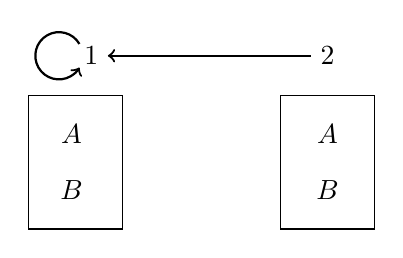
\begin{tikzpicture}
		\node (atom1) at (0,1) {1};
		\node (atom2) at (3,1) {2};
		\node (atom3) at (-0.25,0) {$A$};
		\node (atom4) at (3,0) {$\enot A$};
		\node (atom5) at (-0.25,-0.7) {$\enot B$};
		\node (atom6) at (3,-0.7) {$B$};
		\draw[->, thick] (atom1)+(-0.15,0.15) arc (-330:-30:.3);
		%\draw[->, thick] (atom2)+(0.15,-0.15) arc (-150:150:.3);
		\draw[<-, thick] (atom1) -- (atom2);
		\draw (-0.8,-1.2) rectangle (0.4,0.5);
		\draw (2.4,-1.2) rectangle (3.6,0.5);
	\end{tikzpicture}
	\end{arialabel}
\end{center}

下面是如何从图表中读出该解释的细节。它只包含两个世界，1 和 2。世界之间的箭头表示可及关系。所以 1 和 2 都可及 1，但 1 和 2 都不可及 2。每个世界旁边的方框让我们知道哪些原子语句在每个世界中为真：$A$ 在 1 中为真但在 2 中为假；$B$ 在 1 中为假但在 2 中为真。你只能在这些方框中写入一个原子语句或一个原子语句的否定。我们可以据此推算出更复杂的语句在每个世界中得到什么真值。例如，在这个解释下，以下所有语句在 $w_1$ 中都为真：
\[
A\eand\enot B,\qquad B\eif A,\qquad \ediamond A,\qquad \ebox\enot B
\]
如果你不喜欢用图示的方式思考，那么你也可以像这样呈现一个解释：

\begin{ekey}
	\item[W]$1,2$
	\item[R]$\langle 1,1\rangle, \langle 2,1\rangle$
	\item[\nu]$\nu_{1}(A)=T, \nu_{1}(B)=F, \nu_{2}(A)=F, \nu_{2}(B)=T$
\end{ekey}

稍后当我们开始考察\emph{反解释}时，你将有机会自己构造一些解释。

\section{系统 \mlK 的语义}
\label{SemanticsK}

现在我们可以将真值函项逻辑的所有语义概念扩展到模态逻辑：
\factoidbox{


\begin{factoiditems}
		\item $\metav{A}_1,\metav{A}_2, \dots
		\metav{A}_n\therefore\metav{C}$ 是\define{模态有效的（modally valid）}\ifeff{}
		在所有解释的所有世界中，不存在
		$\metav{A}_1,\metav{A}_2, \dots \metav{A}_n$ 全部为真而
		$\metav{C}$ 为假的情况。

		\item $\metav{A}$ 是\define{模态永真式（modal truth）}\ifeff{} $\metav{A}$
		在所有解释的所有世界中都为真。

		\item $\metav{A}$ 是\define{模态矛盾式（modal contradiction）}\ifeff{}
		$\metav{A}$ 在所有解释的所有世界中都为假。

		\item $\metav{A}$ 是\define{模态可满足的（modally satisfiable）}\ifeff{}
		$\metav{A}$ 在某个解释的某个世界中为真。
	\end{factoiditems}


		}
（从现在起，我们将省略明确的“模态”限定词，因为它们可以默认理解。）

我们也可以扩展 $\entails$ 的使用。但正如我们对 $\proves$ 所做的那样，我们需要再次添加下标。所以，当我们想表达 $\metav{A}_1,\metav{A}_2, \dots \metav{A}_n\therefore\metav{C}$ 有效时，我们将写作：$\metav{A}_1,\metav{A}_2, \dots \metav{A}_n\entails_\mlK\metav{C}$。

让我们通过给出一些反解释来更好地感受这种语义。考虑以下（错误的）主张：
\[\enot A\entails_\mlK \enot \ediamond A\]
为了给出这个主张的反解释，我们需要构造一个解释，使得 $\enot A$ 在某个世界 $w$ 上为真，而 $\enot\ediamond A$ 在 $w$ 上为假。这里有一个这样的解释，用图表表示如下：


\begin{center}
\begin{arialabel}{数字 1 和 2 由从 1 指向 2 的箭头连接。节点 1 标为 not-A，节点 2 标为 A。}
	\begin{tikzpicture}
		\node (atom1) at (0,1) {1};
		\node (atom2) at (3,1) {2};
		\node (atom3) at (-0.25,0) {$\enot A$};
		\node (atom4) at (3,0) {$A$};
		\draw[->, thick] (atom1) -- (atom2);
		\draw (-0.8,-0.6) rectangle (0.4,0.5);
		\draw (2.4,-0.6) rectangle (3.6,0.5);
	\end{tikzpicture}
\end{arialabel}
\end{center}


很容易看出，这将作为我们主张的反解释。首先，$\enot A$ 在世界 $1$ 上为真。其次，$\enot\ediamond A$ 在 $1$ 上为假：$A$ 在 $2$ 上为真，且 $2$ 可由 $1$ 可及。所以，在这个解释中存在某个世界，其中 $\enot A$ 为真而 $\enot\ediamond A$ 为假，因此并非 $\enot A\entails_\mlK\enot\ediamond A$。

为什么我们选择下标 \mlK？嗯，事实表明，系统 \mlK 与我们刚刚给出的有效性定义之间存在一个重要关系。具体来说，我们有以下两个结果：


\begin{compactlist}
	\item 如果 $\metav{A}_1,\metav{A}_2, \dots \metav{A}_n\proves_\mlK\metav{C}$，那么 $\metav{A}_1,\metav{A}_2, \dots \metav{A}_n\entails_\mlK\metav{C}$
	\item 如果 $\metav{A}_1,\metav{A}_2, \dots \metav{A}_n\entails_\mlK\metav{C}$，那么 $\metav{A}_1,\metav{A}_2, \dots \metav{A}_n\proves_\mlK\metav{C}$
\end{compactlist}


第一个结果被称为\emph{可靠性}结果，因为它告诉我们系统 \mlK 的规则是好的、可靠的规则：如果你能通过使用系统 \mlK 给出一个证明来证成一个论证，那么该论证确实是有效的。第二个结果被称为\emph{完备性}结果，因为它告诉我们系统 \mlK 的规则足够广泛，能捕捉所有有效论证：如果一个论证是有效的，那么就有可能用系统 \mlK 给出一个证明来证成它。

然而，陈述这些结果是一回事，证明它们又是另一回事。不过，我们不会在这里尝试证明它们。但可靠性证明背后的想法或许能让严格子证明的工作原理更清晰。

在严格子证明中，我们不能使用严格子证明之外的任何内容，除了我们使用 \ebox E 导入严格子证明的东西。如果我们已经假设或证明了 $\ebox \metav{A}$，那么通过 \ebox E，我们可以在严格子证明中使用 $\metav{A}$。而在系统 \mlK 中，这是将公式导入严格子证明的唯一方式。因此，在严格子证明内部所能证明的一切，都必须从在严格子证明外部我们有 $\ebox \metav{A}$ 的那些公式 $\metav{A}$ 推得。假设我们正在推理某个解释中一个可能世界上的真值。如果我们知道 $\ebox\metav{A}$ 在那个可能世界上为真，我们就知道 $\metav{A}$ 在所有可及世界上都为真。所以，在严格子证明内部所证明的一切在所有可及可能世界上都为真。这就是为什么 \ebox I 是一条可靠的规则。

\section{系统 \mlT 的语义}
\label{SemanticsT}

刚才我们说系统 \mlK 是可靠且完备的。那么我们考察过的其他模态系统，即系统 \mlT、\mlSfour 和 \mlSfive，情况又如何呢？嗯，相对于我们上面给出的有效性定义，它们都是\emph{不可靠的}。例如，所有这些系统都允许我们从 $\ebox A$ 推断 $A$，尽管 $\ebox A\nentails_\mlK A$。

这是否意味着这些系统毫无用处？完全不是！这些系统只是\emph{相对于我们上面给出的有效性定义}是不可靠的。（或者用符号来说，它们相对于 $\entails_\mlK$ 是不可靠的。）所以，当我们处理这些更强的模态系统时，我们只需要修改我们的有效性定义以适应。这正是可及关系真正派上用场的地方。

当我们引入可及关系这个概念时，我们说过它可以是任何你喜欢的世界之间的关系：你可以让它把每个世界与每个世界关联起来，不把任何世界与任何世界关联起来，或者介于两者之间。这就是我们在定义 $\entails_\mlK$ 时看待可及关系的方式。但如果我们愿意，我们可以开始对可及关系施加一些限制。特别是，我们可以坚持它必须是\emph{自反的}：
\[\forall w\, Rww\]
用自然语言说：每个世界都可及自身。或者用相对可能性来说：每个世界相对于自身都是可能的。如果我们施加这个限制，就可以引入一个新的后承关系 $\entails_\mlT$，定义如下：
\factoidbox{
	$\metav{A}_1,\metav{A}_2, \dots \metav{A}_n\entails_\mlT \metav{C}$ \ifeff{} 在任何\emph{具有自反可及关系的}解释中，都不存在一个世界，使得 $\metav{A}_1,\metav{A}_2, \dots \metav{A}_n$ 都为真而 $\metav{C}$ 为假
}
我们在 $\entails$ 上附加了 \mlT{} 下标，因为系统 \mlT{} 相对于这个新的有效性定义是可靠且完备的：


\begin{compactlist}
	\item 如果 $\metav{A}_1,\metav{A}_2, \dots \metav{A}_n\proves_\mlT\metav{C}$，那么 $\metav{A}_1,\metav{A}_2, \dots \metav{A}_n\entails_\mlT\metav{C}$
	\item 如果 $\metav{A}_1,\metav{A}_2, \dots \metav{A}_n\entails_\mlT\metav{C}$，那么 $\metav{A}_1,\metav{A}_2, \dots \metav{A}_n\proves_\mlT\metav{C}$
\end{compactlist}


和以前一样，我们不会试图证明这些可靠性和完备性结果。不过，相对容易看出，坚持可及关系必须是自反的将如何为 R\mlT{} 规则提供依据：
\factoidbox{


\begin{fitchproof}
			\have[m]{m}{\ebox \metav{A}}
			\have[\, ]{n}{\metav{A}}\rt{m}
	\end{fitchproof}


}
为了看清这一点，只需设想试图为以下断言构造一个反解释：
\[
	\ebox \metav{A}\entails_\mlT \metav{A}
\]
我们需要构造一个世界 $w$，使得在 $w$ 上 $\ebox \metav{A}$ 为真，而 $\metav{A}$ 为假。现在，如果 $\ebox \metav{A}$ 在 $w$ 上为真，那么 $\metav{A}$ 必须在 $w$ 所可及的每一个世界上为真。但由于可及关系是自反的，$w$ 可及 $w$。因此 $\metav{A}$ 必须在 $w$ 上为真。但现在 $\metav{A}$ 在 $w$ 上必定既\emph{为真}又\emph{为假}。矛盾！

\section{\mlSfour 的语义}
\label{SemanticsS4}

我们还可以如何调整有效性的定义？我们也可以规定可及关系必须是\emph{传递的}：
\[\forall w_1\forall w_2\forall w_3 ((Rw_1w_2 \eand Rw_2w_3)\eif Rw_1w_3)\]
用自然语言说：如果 $w_1$ 可及 $w_2$，且 $w_2$ 可及 $w_3$，那么 $w_1$ 可及 $w_3$。或者用相对可能性来说：如果 $w_3$ 相对于 $w_2$ 是可能的，且 $w_2$ 相对于 $w_1$ 是可能的，那么 $w_3$ 相对于 $w_1$ 就是可能的。如果我们在可及关系上加上这个限制，我们就可以引入一个新的后承关系 $\entails_\mlSfour$，定义如下：
\factoidbox{
	$\metav{A}_1,\metav{A}_2, \dots \metav{A}_n\entails_\mlSfour \metav{C}$ \ifeff{} 在任何\emph{具有自反且传递的可及关系的}解释中，都不存在一个世界，使得 $\metav{A}_1,\metav{A}_2, \dots \metav{A}_n$ 都为真而 $\metav{C}$ 为假
}
我们在 $\entails$ 上附加了 \mlSfour{} 下标，因为系统 \mlSfour{} 相对于这个新的有效性定义是可靠且完备的：


\begin{compactlist}
	\item 如果 $\metav{A}_1,\metav{A}_2, \dots \metav{A}_n\proves_\mlSfour\metav{C}$，那么 $\metav{A}_1,\metav{A}_2, \dots \metav{A}_n\entails_\mlSfour\metav{C}$
	\item 如果 $\metav{A}_1,\metav{A}_2, \dots \metav{A}_n\entails_\mlSfour\metav{C}$，那么 $\metav{A}_1,\metav{A}_2, \dots \metav{A}_n\proves_\mlSfour\metav{C}$
\end{compactlist}


和以前一样，我们不会试图证明这些可靠性和完备性结果。不过，相对容易看出，坚持可及关系必须是传递的将如何为 \mlSfour{} 规则提供依据：
\factoidbox{


\begin{fitchproof}
			\have[m]{m}{\ebox\metav{A}}
			\open
			\hypo[\ ]{k}{\ebox}\AS
			\have[\ ]{n}{\ebox\metav{A}}\rfour{m}
	\end{fitchproof}


}
请记住，严格子证明背后的思想是，它们是用来证明在所有可及世界中必然为真的事物的方法。所以 R$\mathbf{4}$ 规则意味着，每当 $\ebox \metav{A}$ 为真时，$\ebox \metav{A}$ 在每一个可及世界中也都必须为真。换句话说，我们必定有 $\ebox\metav{A} \entails_\mlSfour \ebox\ebox\metav{A}$。

为了看清这一点，只需设想试图为以下主张构造一个反解释：
\[\ebox\metav{A} \entails_\mlSfour \ebox \ebox \metav{A}\]
我们需要构造一个世界 $w_1$，使得在 $w_1$ 上 $\ebox\metav{A}$ 为真，而 $\ebox \ebox \metav{A}$ 为假。现在，如果 $\ebox \ebox \metav{A}$ 在 $w_1$ 上为假，那么 $w_1$ 必定可及某个世界 $w_2$，使得在 $w_2$ 上 $\ebox\metav{A}$ 为假。同样，如果 $\ebox \metav{A}$ 在 $w_2$ 上为假，那么 $w_2$ 必定可及某个世界 $w_3$，使得在 $w_3$ 上 $\metav{A}$ 为假。我们刚刚说过，$w_1$ 可及 $w_2$，且 $w_2$ 可及 $w_3$。因此，由于我们现在坚持可及关系是传递的，$w_1$ 必定可及 $w_3$。又因为 $\ebox\metav{A}$ 在 $w_1$ 上为真，且 $w_3$ 从 $w_1$ 可及，由此得出 $\metav{A}$ 在 $w_3$ 上必定为真。因此 $\metav{A}$ 在 $w_3$ 上既\emph{为真}又\emph{为假}。矛盾！

\section{\mlSfive 的语义}
\label{SemanticsS5}

让我们对可及关系再施加一个限制。这次，让我们坚持它也必须是\emph{对称的}：
\[\forall w_1\forall w_2(Rw_1w_2 \eif Rw_2w_1)\]
用自然语言说：如果 $w_1$ 可及 $w_2$，那么 $w_2$ 可及 $w_1$。或者用相对可能性来说：如果 $w_2$ 相对于 $w_1$ 是可能的，那么 $w_1$ 相对于 $w_2$ 也是可能的。逻辑学家将自反、对称且传递的关系称为\emph{等价关系}。我们现在可以定义一个新的后承关系 $\entails_\mlSfive $，如下所示：
\factoidbox{
	$\metav{A}_1,\metav{A}_2, \dots \metav{A}_n\entails_\mlSfive  \metav{C}$ \ifeff{} 在任何\emph{可及关系是等价关系的}解释中，都不存在一个世界，使得 $\metav{A}_1,\metav{A}_2, \dots \metav{A}_n$ 全部为真而 $\metav{C}$ 为假
}
我们在 $\entails$ 上附加了 \mlSfive{} 下标，因为系统 \mlSfive{} 相对于这个新的有效性定义是可靠且完备的：


\begin{compactlist}
	\item 如果 $\metav{A}_1,\metav{A}_2, \dots \metav{A}_n\proves_\mlSfive \metav{C}$，那么 $\metav{A}_1,\metav{A}_2, \dots \metav{A}_n\entails_\mlSfive \metav{C}$
	\item 如果 $\metav{A}_1,\metav{A}_2, \dots \metav{A}_n\entails_\mlSfive \metav{C}$，那么 $\metav{A}_1,\metav{A}_2, \dots \metav{A}_n\proves_\mlSfive \metav{C}$
\end{compactlist}


和之前一样，我们不会在这里尝试证明这些可靠性和完备性结果。不过，相对容易看出，坚持可及关系必须是等价关系将如何为 R$\mathbf{5}$ 规则提供依据：
\factoidbox{


\begin{fitchproof}
			\have[m]{m}{\enot\ebox \metav{A}}
			\open
			\hypo[\ ]{k}{\ebox}\AS
			\have[\, ]{n}{\enot\ebox\metav{A}}\rfive{m}
	\end{fitchproof}


}
该规则说的是，如果 $\metav{A}$ 并非必然，即在某个可及世界中为假，那么它在任何可及的可能世界中也都并非必然，也就是说，我们有 $\enot\ebox \metav{A} \proves_\mlSfive  \ebox\enot\ebox \metav{A}$。

为了看清这一点，只需设想试图为以下主张构造一个反解释：
\[
	\enot\ebox\metav{A} \entails_\mlSfive  \ebox \enot\ebox \metav{A}
\]
我们需要构造一个世界 $w_1$，使得在 $w_1$ 上 $\enot\ebox\metav{A}$ 为真，而 $\ebox \enot\ebox \metav{A}$ 为假。
现在，如果 $\enot\ebox\metav{A}$ 在 $w_1$ 上为真，那么 $w_1$ 必定可及某个世界 $w_2$，使得在 $w_2$ 上 $\metav{A}$ 为假。同样地，如果 $\ebox \enot\ebox \metav{A}$ 在 $w_1$ 上为假，那么 $w_1$ 必定可及某个世界 $w_3$，使得在 $w_3$ 上 $\enot\ebox \metav{A}$ 为假。既然我们现在坚持可及关系是一种等价关系，因而具有对称性，我们就可以推断 $w_3$ 可及 $w_1$。于是，$w_3$ 可及 $w_1$，且 $w_1$ 可及 $w_2$。再次利用我们现在坚持可及关系是一种等价关系（因而具有传递性）这一点，我们可以推断 $w_3$ 可及 $w_2$。但我们之前说过，在 $w_3$ 上 $\enot\ebox \metav{A}$ 为假，这意味着 $\metav{A}$ 在 $w_3$ 所可及的每一个世界上都为真。因此 $\metav{A}$ 在 $w_2$ 上既\emph{为真}又\emph{为假}。矛盾！

在 $\entails_\mlSfive $ 的定义中，我们规定可及关系必须是一个等价关系。但事实证明，还有另一种方法可以得到适合 \mlSfive 的有效性概念。我们不必规定可及关系是等价关系，而是可以规定它是一种\emph{全通}关系：
\[\forall w_1\forall w_2\, Rw_1w_2\]
用自然语言说：每个世界可及每个世界。或者用相对可能性来说：每个世界相对于每个世界都是可能的。使用这种对可及关系的限制，我们可以像下面这样定义 $\entails_\mlSfive $：
\factoidbox{
	$\metav{A}_1,\metav{A}_2, \dots \metav{A}_n\entails_\mlSfive  \metav{C}$ \ifeff{} 在任何\emph{具有全通可及关系}的解释中，都不存在一个世界，使得 $\metav{A}_1,\metav{A}_2, \dots \metav{A}_n$ 全部为真而 $\metav{C}$ 为假。
}
如果我们这样定义 $\entails_\mlSfive $，对于 \mlSfive 我们仍然会得到相同的可靠性和完备性结果。这告诉我们什么？嗯，这意味着，如果我们要处理的必然性概念认为\emph{每一个}世界都相对于\emph{每一个}世界是可能的，那么我们就应该使用 \mlSfive。更进一步，大多数哲学家都假定，他们最关心的那些必然性概念，比如\emph{逻辑必然性}和\emph{形而上学必然性}，恰恰就是这种类型。因此 \mlSfive{} 是大多数哲学家大多数时候使用的模态逻辑系统。

\practiceproblems

\problempart
给出下列错误主张的反解释：


\begin{compactlist}
	\item $\enot P \entails_\mlK \enot\ediamond P$
	\item $\ebox(P \eor Q)\entails_\mlK \ebox P \eor \ebox Q$
	\item $\entails_\mlK \enot \ebox (A\eand \enot A)$
	\item $\ebox A\entails_\mlK A$
\end{compactlist}

\problempart
给出下列错误主张的反解释：


\begin{compactlist}
	\item $\ediamond A\entails_\mlSfour \ebox\ediamond A$
	\item $\ediamond A, \ebox (\ediamond A \eif B)\entails_\mlSfour\ebox B$
\end{compactlist}

\problempart
给出下列错误主张的反解释：


\begin{compactlist}
	\item $\ebox (M\eif O),\ediamond M\entails_\mlT O$
	\item $\ebox A\entails_\mlT \ebox \ebox A$
\end{compactlist}

\section*{延伸阅读}

模态逻辑是逻辑学中一个庞大的子领域。我们仅仅触及了皮毛。如果你想了解更多关于模态逻辑的内容，可以参考以下教科书：

\begin{itemize}
	\item George E. Hughes 与 Max J. Cresswell 合著，《模态逻辑新导论》（\textit{A New Introduction to Modal Logic}），牛津：Routledge 出版社，1996年。
	\item Graham Priest 著，《非经典逻辑导论》（\textit{An Introduction to Non-Classical Logic}），第二版，剑桥：剑桥大学出版社，2008年。
	\item James W. Garson 著，《面向哲学家的模态逻辑》（\textit{Modal Logic for Philosophers}），第二版，剑桥：剑桥大学出版社，2013年。
\end{itemize}

这些作者都没有完全按照我们的方式来构建他们的模态证明系统，但最接近的构建方式是由 Garson 给出的。
%!TEX root = forallxyyc.tex
\part{元理论}
\label{ch.normalform}
\addtocontents{toc}{\protect\mbox{}\protect\hrulefill\par}

\chapter{范式}\label{c:NormalForms}

\section{析取范式}\label{s:DNFDefined}

有时，考虑形式特别简单的语句是很有用的。例如，我们可以考虑那些 $\enot$ 只出现在原子语句之前的语句，或者那些只用 $\eand$ 将原子语句和带否定的原子语句组合起来的语句。一种相对通用但仍保持简单的形式是：一个语句是若干原子语句或带否定的原子语句的合取式的析取。当构造这样一个语句时，我们从原子语句开始，然后（可能）附加否定，接着（可能）用 $\eand$ 组合，最后（可能）用 $\eor$ 组合。

我们说一个语句是 \define{析取范式（disjunctive normal form）} \emph{\ifeff} 它满足以下所有条件：

\begin{compactlist}
		\item[(\textsc{dnf1})] 除了否定、合取和析取外，语句中不出现其他联结词；
		\item[(\textsc{dnf2})] 每个否定的出现都具有最小辖域（即，任何“$\enot$”都紧跟着一个原子语句）；
		\item[(\textsc{dnf3})] 任何析取的辖域内都不出现合取。
	\end{compactlist}

\newglossaryentry{disjunctive normal form}{
  name = 析取范式,
  text = 析取范式,
  description = {一种语句，它是若干原子语句或带否定的原子语句的合取式的析取}
}
所以，以下是一些属于析取范式的语句：
\begin{align*}
  & A \\
  & (A \eand \lnot B \eand C)\\
  & (A \eand B) \eor (A \eand \enot B)\\
  & (A \eand B) \eor (A \eand  B \eand C \eand \enot D \eand \enot E)\\
  & A \eor (C \eand \enot P_{234} \eand P_{233} \eand Q) \eor \enot B
\end{align*}
注意，我们这里暂时打破了本书的一项原则，\emph{临时}允许自己采用宽松的括号约定，允许合取式和析取式具有任意长度。这些约定使得判断一个语句是否属于析取范式变得更加容易。后续我们将继续采用这些宽松约定，不再另行说明。

为了进一步阐明析取范式的概念，我们将引入更多记号。我们用“$\pm\metav{A}$”表示 $\metav{A}$ 是一个原子语句，它前面可能带有一个否定符号，也可能没有。那么，一个属于析取范式的语句具有以下形状：
	$$(\pm \metav{A}_1 \land \ldots \land \pm \metav{A}_i) \lor (\pm \metav{A}_{i+1} \land \ldots \land \pm\metav{A}_j) \lor \ldots \lor (\pm\metav{A}_{m+1} \land \ldots \land \pm \metav{A}_n)$$
我们现在知道了什么是属于析取范式的语句。我们旨在证明的结果是：
	\factoidbox{\label{thm:dnf}\textbf{析取范式定理。} 对任意语句，都存在一个与之逻辑等价的、属于析取范式的语句。
	}
\section{通过真值表证明析取范式定理}
\label{s:DNFTruthTable}

我们对析取范式定理的第一个证明使用了真值表。我们将首先举例说明如何找出等价的析取范式语句，然后再将这一示例转化为严格的证明。

假设我们有一个语句 $\metav{S}$，它包含三个原子语句“$A$”、“$B$” 和 “$C$”。首先要做的是为 $\metav{S}$ 画出一张完整的真值表。结果可能如下：

\begin{center}
\begin{tabular}{c c c | c}
$A$ & $B$ & $C$ & $\metav{S}$\\
\hline
 T & T & T & T \\
 T & T & F & F \\
 T & F & T & T \\
 T & F & F & F \\
 F & T & T & F \\
 F & T & F & F \\
 F & F & T & T \\
 F & F & F & T
\end{tabular}
\end{center}

%Now, consider a sentence, whose only connectives are negations and conjunctions, where no connective occurs within the scope of any negation, e.g.:
%	$$A \eand \enot B \eand C$$
%This sentence is true when, and only when, “$A$” is true, “$B$” is false and “$C$” is true. Similarly, the sentence:
%	$$\enot A \eand \enot B \eand C$$
%this is true when, and only when, “$A$” is false, “$B$” is false and “$C$” is true.
%
%A disjunction is true when, and only when, at least one of the disjuncts is true. So if we write down a disjunction of sentences of the above form, perhaps
%	$$(A \eand \enot B \eand C) \eor (\enot A \eand \enot B \eand C)$$
%then it will be true on exactly \emph{two} lines of the truth table which describes all possible valuations of “$A$”, “$B$” and “$C$”.
%
恰巧，$\metav{S}$ 在其真值表的四行上为真，即第 1、3、7 和 8 行。对应于每一行，我们将写下四个只包含否定和合取作为联结词的语句，并且其中每个否定的辖域都保持最小：

\begin{compactlist}
		\item  “$A \eand B \eand C$”\hfill 该式在第 1 行为真（且仅当该行）
		\item “$A \eand \enot B \eand C$” \hfill 该式在第 3 行为真（且仅当该行）
		\item “$\enot A \eand \enot B \eand C$” \hfill 该式在第 7 行为真（且仅当该行）
		\item “$\enot A \eand \enot B \eand \enot C$” \hfill 该式在第 8 行为真（且仅当该行）
	\end{compactlist}

现在我们用 $\eor$ 将所有合取式组合起来：
$$(A \eand B \eand C) \eor (A \eand \enot B \eand C) \eor (\enot A \eand \enot B \eand C) \eor (\enot A \eand \enot B \eand \enot C)$$\label{longDNF}
这样就得到了一个析取范式语句，它恰好在那些至少有一个析取支为真的行上为真，即在（且仅在）第 1、3、7 和 8 行为真。因此，这个语句与 $\metav{S}$ 具有完全相同的真值表。于是我们得到了一个与 $\metav{S}$ 逻辑等价的析取范式语句，这正是我们想要的！

我们刚才采用的策略并不依赖于 $\metav{S}$ 的具体细节；它是完全通用的。因此，我们可以利用它来给出析取范式定理的一个简单证明。

任选一个语句 $\metav{S}$，并令 $\metav{A}_1, \ldots, \metav{A}_n$ 为出现在 $\metav{S}$ 中的所有原子语句。为得到一个逻辑等价于 $\metav{S}$ 的析取范式语句，我们需要考察 $\metav{S}$ 的真值表。有两种情况需要考虑：

\begin{numberlist}
		\item \emph{$\metav{S}$ 在其真值表的每一行上均为假。} 那么 $\metav{S}$ 是一个矛盾式。在这种情况下，矛盾式 $(\metav{A}_1 \eand \enot \metav{A}_1)$ 是一个析取范式语句，且逻辑等价于 $\metav{S}$。
		\item \emph{$\metav{S}$ 在其真值表的至少一行上为真。}
		对于真值表的每一行 $i$，令 $\metav{B}_i$ 为一个形如
		$$(\pm\metav{A}_1 \land \ldots \land \pm\metav{A}_n)$$
		的合取式，其中决定是否在每一个原子语句前添加否定的规则如下：
			\begin{itemize}
				\item $\metav{A}_m$ 是 $\metav{B}_i$ 的一个合取支 \emph{\ifeff} $\metav{A}_m$ 在第 $i$ 行为真。
				\item $\enot\metav{A}_m$ 是 $\metav{B}_i$ 的一个合取支 \emph{\ifeff} $\metav{A}_m$ 在第 $i$ 行为假。
			\end{itemize}
		根据这些规则，$\metav{B_i}$ 在且仅在真值表考虑 $\metav{A}_1$, \ldots, $\metav{A}_n$ 所有可能赋值（即 $\metav{S}$ 的真值表）的第 $i$ 行上为真。

		接下来，令 $i_1$, $i_2$, \dots, $i_m$ 为真值表中 $\metav{S}$ \emph{为真} 的那些行的编号。现在令 $\metav{D}$ 为如下语句：
		$$\metav{B}_{i_1} \eor \metav{B}_{i_2} \eor \ldots \eor \metav{B}_{i_m}$$
		既然 $\metav{S}$ 在其真值表的至少一行上为真，那么 $\metav{D}$ 就是良定义的；在极限情况下，即 $\metav{S}$ 在其真值表上恰好只在一行上为真时，$\metav{D}$ 就直接是某个 $\metav{B}_{i_1}$。

		根据构造，$\metav{D}$ 是析取范式语句。此外，根据构造，对于真值表的每一行 $i$：$\metav{S}$ 在该行上为真 \emph{\ifeff} $\metav{D}$ 的某个析取支（即 $\metav{B_i}$）在且仅在该行上为真。因此，$\metav{S}$ 和 $\metav{D}$ 具有相同的真值表，从而逻辑等价。
	\end{numberlist}

	这两种情况已穷尽所有可能，无论如何，我们都得到了一个逻辑等价于 $\metav{S}$ 的析取范式语句。

于是我们证明了析取范式定理。不过，在我们进一步讨论之前，应当立即指出，我们因此回到了对（真值函项逻辑）语句的严格定义，根据该定义，可以假定任一合取式恰有两个合取支，任一个析取式恰有两个析取支。

\section{合取范式}
\label{s:CNF}

本章至此我们讨论的是\emph{析取}范式。存在所谓的\emph{合取范式}，可能并不令人意外。

合取范式 的定义与析取范式的定义完全类似。确切地说，一个语句是合取范式语句 \emph{\ifeff} 它满足以下所有条件：

\begin{compactlist}
		\item[(\textsc{cnf1})] 除了否定、合取和析取之外，该语句中不出现任何其他联结词；
		\item[(\textsc{cnf2})] 每个否定的出现都具有最小辖域；
		\item[(\textsc{cnf3})] 任何合取的辖域内都不出现析取。
	\end{compactlist}

\newglossaryentry{conjunctive normal form}{
  name = 合取范式,
  text = 合取范式,
  description = {一种语句，它是若干原子语句或带否定的原子语句的析取式的合取}
}
一般而言，一个合取范式语句形如
	$$(\pm \metav{A}_1 \lor \ldots \lor \pm \metav{A}_i) \land (\pm \metav{A}_{i+1} \lor \ldots \lor \pm\metav{A}_j) \land \ldots \land (\pm\metav{A}_{m+1} \lor\ldots \lor \pm \metav{A}_n)$$
其中每个 $\metav{A}_k$ 都是一个原子语句。

我们现在可以证明另一个范式定理：
	\factoidbox{\label{thm:cnf}\textbf{合取范式定理。} 对于任一语句，都存在一个与其逻辑等价的合取范式语句。}

	给定一个真值函项逻辑语句 $\metav{S}$，我们首先写下 $\metav{S}$ 的完整真值表。

	如果 $\metav{S}$ 在真值表的\emph{每一行}上都为真，那么 $\metav{S}$ 与 $(\metav{A}_1 \eor \enot \metav{A}_1)$ 逻辑等价。

	如果 $\metav{S}$ 在真值表的\emph{至少一行}上为假，那么，对于真值表中 $\metav{S}$ 为假的每一行，写下在该行上（且仅在该行上）为\emph{假}的析取式 $(\pm\metav{A}_1 \eor \ldots \eor \pm\metav{A}_n)$。令 $\metav{C}$ 为所有这些析取式的合取；根据构造，$\metav{C}$ 是合取范式语句，并且 $\metav{S}$ 与 $\metav{C}$ 逻辑等价。

\practiceproblems
\problempart
\label{pr.DNF}
考虑以下语句：

\begin{compactlist}
		\item $(A \eif \enot B)$
		\item $\enot (A \eiff B)$
		\item $(\enot A \eor \enot (A \eand B))$
		\item $(\enot (A \eif B ) \eand (A \eif C))$
		\item $(\enot (A \eor B) \eiff ((\enot C \eand \enot A) \eif \enot B))$
		\item $((\enot (A \eand \enot B) \eif C) \eand \enot (A \eand D))$
	\end{compactlist}

        对每一个语句，分别找出一个逻辑等价的析取范式语句和一个逻辑等价的合取范式语句。

\chapter{功能完全性}\label{c:FunctionalCompleteness}

在我们的联结词中，$\enot$ 仅作用于一个句子，其他联结词都恰好组合两个句子。我们也可以引入 $n$ 元联结词的概念。例如，我们可以考虑一个三元联结词 “$\heartsuit$”，并规定它具有以下特征真值表：

\begin{center}
\begin{tabular}{c c c | c}
$A$ & $B$ & $C$ & $\heartsuit(A,B,C)$\\
\hline
 T & T & T & F \\
 T & T & F & T \\
 T & F & T & T \\
 T & F & F & F \\
 F & T & T & F \\
 F & T & F & T \\
 F & F & T & F \\
 F & F & F & F
\end{tabular}
\end{center}

可能这个新联结词不对应任何自然的英语表达式（至少不像 “$\eand$” 对应“and”那样）。但问题随之产生：如果我们想使用具有这个特征真值表的联结词，是否必须在真值函项逻辑中添加一个\emph{新}联结词？还是说我们可以用\emph{已有}的联结词来达到目的（就像我们可以用已有联结词表达“既不……也不……”那样）？

让我们更精确地表述这个问题。我们说一组联结词是\define{联合功能完备的} \emph{\ifeff}，对于任何可能的真值表，都存在一个只包含这些联结词的句子具有该真值表。

\newglossaryentry{functionally complete}{
  name = {功能完备性},
  text = {功能完备的},
  description = {联结词集合的一个性质，该性质成立 \ifeff{} 每个可能的真值表都是某个仅包含那些联结词的句子的真值表}}

一般要点是，当我们掌握了一些联合功能完备的联结词，就没有哪个特征真值表是我们无法把握的。事实上，我们很幸运。
	\factoidbox{\label{thm:ExpressiveAdequacy}\textbf{功能完备性定理。}
真值函项逻辑的联结词是联合功能完备的。事实上，以下几对联结词都是联合功能完备的：

\begin{compactlist}
\item\label{expressive:eor} “$\enot$” 和 “$\eor$”
\item\label{expressive:eand} “$\enot$” 和 “$\eand$”
\item\label{expressive:eif} “$\enot$” 和 “$\eif$”
\end{compactlist}
}

给定任何真值表，我们可以使用\cref{c:NormalForms}中通过真值表证明析取范式定理（或合取范式定理）的方法，写下一个具有相同真值表的模式。例如，运用证明析取范式定理的真值表方法，我们发现以下模式具有与上面$\heartsuit(A,B,C)$相同的特征真值表：
		$$(A \eand B \eand \enot C) \eor (A \eand \enot B \eand C) \eor (\enot A \eand B \eand \enot C)$$
由此可见，真值函项逻辑的联结词是联合功能完备的。我们现在证明每一个辅助结果。

\emph{辅助结果1：“$\enot$”和“$\eor$”的功能完备性。}注意，使用证明析取范式定理的真值表方法生成的模式将只包含联结词“$\enot$”、“$\eand$”和“$\eor$”。因此，只需证明存在一个只包含“$\enot$”和“$\eor$”的等价模式即可。为达此目的，我们只需注意到：
		\begin{align*}
		(\metav{A} \eand \metav{B}) & \Leftrightarrow \enot(\enot \metav{A} \eor\enot \metav{B})
		\end{align*}
		是逻辑等价的。\footnote{这里我们采用一个约定：称$\metav{A}$和$\metav{B}$等价可缩写为$\metav{A} \Leftrightarrow \metav{B}$。注意“$\Leftrightarrow$” \emph{不是}像“$\eiff$”那样的联结词，而是像“$\entails$”一样的元语言符号；比较\cref{entails-v-iff}中对“$\entails$”和“$\eiff$”的讨论。}

\emph{辅助结果2：“$\enot$”和“$\eand$”的功能完备性。}与辅助结果1完全相同，利用以下事实：
		\begin{align*}
		(\metav{A} \eor \metav{B}) & \Leftrightarrow \enot(\enot \metav{A} \eand\enot \metav{B})
		\end{align*}
		是逻辑等价的。

\emph{辅助结果3：“$\enot$”和“$\eif$”的功能完备性。}与辅助结果1完全相同，但改用以下等价式：
		\begin{align*}
		(\metav{A} \eor \metav{B}) &\Leftrightarrow (\enot \metav{A} \eif \metav{B})\\
		(\metav{A} \eand \metav{B}) &\Leftrightarrow \enot(\metav{A} \eif \enot\metav{B})
		\end{align*}
或者，我们可以直接依赖另外两个辅助结果之一，并且（反复地）只调用这两个等价式中的一个。

总之，我们\emph{从不必须}在真值函项逻辑中添加新的联结词。事实上，我们已有的联结词中已经存在冗余：如果我们当初真的力求精简，本可以只用两个联结词就够了。

\ifHTMLtarget
\section{单独功能完备的联结词}
\else
\section[单独功能完备的联结词][功能完备的联结词]{单独功能完备的联结词}
\fi

事实上，一些二元联结词是\emph{单独}功能完备的。这些联结词通常不包含在真值函项逻辑中，因为它们使用起来相当繁琐。但它们的存在表明，倘若我们愿意，本可以定义一种功能完备的真值函项语言，它仅包含一个初始联结词。

我们将考虑的第一个此类联结词是 “$\uparrow$”，它具有以下特征真值表。

\begin{center}
\begin{tabular}{c c | c}
$\metav{A}$ & $\metav{B}$ & $\metav{A} \mathrel{\uparrow} \metav{B}$\\
\hline
 T & T & F \\
 T & F & T \\
 F & T & T  \\
 F & F & T
\end{tabular}
\end{center}

这通常被称为“谢弗竖线”，得名于亨利·谢弗，他曾用它来展示如何减少 Russell 和 Alfred North Whitehead（阿尔弗雷德·诺思·怀特海）《数学原理》中的逻辑联结词数量。\footnote{Sheffer, “”A set of five independent postulates for Boolean algebras, with application to logical constants'', \textit{Transactions of the American Mathematical Society}~14 (1913), pp. 481--488}（实际上，查尔斯·桑德斯·皮尔士比谢弗早了大约30年就预见到了这一点，但他从未发表其结果；而波兰哲学家爱德华·斯塔姆则比谢弗早两年发表了同样的结果。）\footnote{参见皮尔士约1880年的文章“A Boolian algebra with one constant”，收录于Peirce's \textit{Collected Papers}, vol. 4, pp. 264--5；以及爱德华·斯塔姆，“”\foreignlanguage{german}{Beitrag zur Algebra der Logik}'', \foreignlanguage{german}{\textit{Monatshefte für Mathematik und Physik}}~22 (1911), pp. 137--49。}它也常被称为“与非”，因为它的特征真值表正是“$\eand$”的真值表的否定。
\factoidbox{\label{prop:upexpressive}“$\uparrow$” 自身就是功能完备的。}

功能完备性定理告诉我们，“$\enot$”和“$\eor$”是联合功能完备的。因此，只需证明：给定任何一个只包含这两个联结词的图式，我们都能将其重写为一个只包含“$\uparrow$”的等价图式。于是，与功能完备性定理辅助结果的证明类似，我们只需对辅助结果~\ref*{expressive:eor} 应用以下等价式：
		\begin{align*}
			\enot \metav{A} &\Leftrightarrow (\metav{A} \uparrow \metav{A})\\
			(\metav{A} \eor \metav{B}) & \Leftrightarrow ((\metav{A} \uparrow \metav{A}) \uparrow (\metav{B} \uparrow \metav{B}))
		\end{align*}

类似地，我们可以考虑联结词“$\downarrow$”：

\begin{center}
\begin{tabular}{c c | c}
$\metav{A}$ & $\metav{B}$ & $\metav{A} \mathrel{\downarrow} \metav{B}$\\
\hline
 T & T & F \\
 T & F & F  \\
 F & T & F  \\
 F & F & T
\end{tabular}
\end{center}

这有时被称为“皮尔斯箭头”（皮尔士本人称其为“ampheck”）。不过，更常见的名称是“或非”，因为它的特征真值表是“$\eor$”的否定，即表示“既不……也不……”。
	\factoidbox{
	“$\downarrow$” 自身就是功能完备的。}

与前面关于 $\uparrow$ 的结果证明类似，只不过这里应用的是以下等价式：
		\begin{align*}
			\enot \metav{A} &\Leftrightarrow (\metav{A} \downarrow \metav{A})\\
			(\metav{A} \eand \metav{B}) & \Leftrightarrow ((\metav{A} \downarrow \metav{A}) \downarrow (\metav{B} \downarrow \metav{B}))
		\end{align*}
以及辅助结果~\ref*{expressive:eand}。

\section{功能不完备的情况}

实际上，\emph{仅有的}两种自身功能完备的二元联结词是“$\uparrow$”和“$\downarrow$”。但我们如何证明这一点呢？更一般地说，我们如何证明某些联结词\emph{并非}联合功能完备？

显然，我们需要尝试找出某个真值表，它\emph{无法}仅用给定的联结词来表达。但这需要一些技巧。

为具体起见，让我们考虑“$\eor$”是否自身功能完备的问题。稍加思考便会清楚，并非如此。具体来说，任何仅包含析取的图式，其真值表都不可能和否定式相同，即：

\begin{center}
				\begin{tabular}{c | c}
				$\metav{A}$ & $\enot \metav{A}$\\
				\hline
				 T & F \\
				 F & T
				\end{tabular}
				\end{center}

其直观原因很简单：目标真值表的首行需要取值为假；但任何\emph{仅}包含$\eor$的图式的真值表，其首行总是为真。对于$\eand$、$\eif$和$\eiff$，情况同样如此。
 	\factoidbox{
		“$\eor$”、“$\eand$”、“$\eif$”和“$\eiff$”自身都不是功能完备的。}

事实上，以下结论成立：

\factoidbox{自身功能完备的\emph{仅有的}二元联结词是“$\uparrow$”和“$\downarrow$”。}

当然，这比针对原始联结词的证明要困难。例如，“排斥或”联结词的特征真值表首行并非T，因此上述方法不足以证明它不能表达所有真值表。要证明诸如“$\eiff$”和“$\enot$”\emph{联合}起来也非功能完备，同样更为困难。

\chapter{证明等值式}\label{ch:equivalences}

\section{等值式的可替换性}

回忆一下，从\cref{sec:equivalent}可知，$\metav{P}$ 和 $\metav{Q}$（在真值函项逻辑中）是等价的 \ifeff{} 对每个赋值而言，它们的真值都相同。我们已经见过很多这样的例子，并且用真值表和自然演绎证明来确立这种等价关系。在\cref{c:NormalForms}中，我们甚至证明了每个真值函项逻辑语句都等价于一个合取范式语句和一个析取范式语句。如果 $\metav{P}$ 和~$\metav{Q}$ 等价，那么它们总是具有相同的真值，任意一个都蕴涵另一个，并且从任意一个出发都可以证明另一个。

当然，等价的语句并非同一个语句：语句 $\enot\enot A$ 和~$A$ 可能总是有相同的真值，但第一个以 “$\enot$” 符号开头，而第二个则不然。不过你可能会想，是否总是能用一对等价语句中的一个替换另一个，并且得到的结果也是等价的呢？例如，考虑 $\enot\enot A \eif B$ 和 $A \eif B$。第二个语句正是将第一个语句中的 “$\enot\enot A$” 替换为~“$A$” 得到的。而这两个语句也确实等价。

这是一个普遍事实，并且不难理解原因。在任何赋值下，我们“从内到外”计算一个语句的真值。所以，当要决定 “$\enot\enot A \eif B$” 的真值时，我们首先计算 “$\enot\enot A$” 的真值，整个语句的真值随后就只取决于这个真值（可能是真或假）和语句的其余部分（即~“$B$” 的真值和 “$\eif$” 的真值表）。但是，由于 “$\enot\enot A$” 和~“$A$” 等价，在给定的赋值下它们总是具有相同的真值——因此，用~“$A$” 替换 “$\enot\enot A$” 不会改变整个语句的真值。当然，对于任何其他与 “$\enot\enot A$” 等价的语句，比如 “$A \eand (A \eor A)$”，情况也是如此。

为了一般性地陈述这个结果，我们使用记号 $\metav{R}(\metav{P})$ 来表示一个包含语句 $\metav{P}$ 作为其组成部分的语句。那么 $\metav{R}(\metav{Q})$ 就表示将 $\metav{P}$ 的出现替换为语句~$\metav{Q}$ 后得到的结果。例如，如果 $\metav{P}$ 是语句字母~“$A$”，$\metav{Q}$ 是语句~“$\enot\enot A$”，而 $\metav{R}(\metav{P})$ 是 “$A \eif B$”，那么 $\metav{R}(\metav{Q})$ 就是 “$\enot\enot A \eif B$”。

\factoidbox{如果 $\metav{P}$ 和 $\metav{Q}$ 是等价的，那么 $\metav{R}(\metav{P})$ 和 $\metav{R}(\metav{Q})$ 也是等价的。}

由此事实可知，任何形如 $\metav{R}(\metav{P}) \eiff \metav{R}(\metav{Q})$ 的语句（其中 $\metav{P}$ 和 $\metav{Q}$ 等价）都是重言式。然而，对于不同的~$\metav{R}$，其自然演绎证明将会有很大差异。（作为练习，请给出证明以表明 \begin{align*}
	& \vdash (\enot\enot P \eif Q) \eiff (P \eif Q)  \text{ 和}\\
	& \vdash (\enot\enot P \eand Q) \eiff (P \eand Q)
\end{align*} 是重言式，并比较这两个证明。）

还有另一个事实：如果两个语句 $\metav{P}$ 和~$\metav{Q}$ 是等价的，并且你在 $\metav{P}$ 和 $\metav{Q}$ 中用同一个语句~$\metav{R}$ 替换了某个相同的语句字母，那么得到的结果也是等价的。例如，如果你在 “$A \land B$” 和 “$B \land A$” 两者中都把 “$A$” 替换为，比方说，“$\enot C$”，你会得到 “$\enot C \land B$” 和 “$B \land \enot C$”，而这两者是等价的。我们也可以记录下这一点：

\factoidbox{等价关系在语句字母替换下保持不变，即，如果 $\metav{P}(A)$ 和 $\metav{Q}(A)$ 都包含语句字母~“$A$” 并且是等价的，那么语句 $\metav{P}(\metav{R})$ 和 $\metav{Q}(\metav{R})$（通过在两者中将 “$A$” 替换为 $\metav{R}$ 得到）也是等价的。}

这意味着，一旦我们证明了两条语句是等价的（例如，“$\enot\enot A$” 和 “$A$”，或 “$A \land B$” 和 “$B \land A$”），我们就知道它们所有共同的“实例”也都是等价的。请注意，我们从真值表或自然演绎证明中并不能直接得到这一点。例如，用于证明 “$\enot\enot A$” 和~“$A$” 等价的真值表，并\emph{不}能同时证明 “$\enot\enot(B \eif C)$” 和 “$B \eif C$” 是等价的：前者只需要 2 行，而后者需要~4 行。

\section{等价链}

当你想验证两个语句等价时，当然可以做真值表，或者寻找形式证明。但还有一种更简单的方法，它基于我们刚刚讨论的等价替换原则：依据一个由简单等价关系构成的小型目录，将第一个语句中的部分替换为等价的部分，并不断重复此过程，直到得到第二个语句。

这种证明语句等价的方法是由前一节的两个事实所支撑的。第一个事实告诉我们，\emph{如果}，比如说，$\enot\enot \metav{P}$ 和 $\metav{P}$ 是等价的（对于任意语句 $\metav{P}$），那么在一个语句中用 $\metav{P}$ 替换 $\enot\enot\metav{P}$ 会产生一个等价的语句。第二个事实告诉我们，对于任意语句 $\metav{P}$，$\enot\enot \metav{P}$ 和 $\metav{P}$ \emph{总是}等价的。（一个简单的真值表就能表明 “$\enot\enot A$” 和 “$A$” 是等价的。）根据第二个事实我们知道，无论何时我们将 “$\enot\enot A$” 和 “$A$” 中的 “$A$” 替换为某个语句 $\metav{P}$，得到的两个语句都是等价的。换句话说，从 “$\enot\enot A$” 和 “$A$” 等价以及第二个事实，我们可以得出结论：对于任意语句 $\metav{P}$，$\enot\enot \metav{P}$ 和 $\metav{P}$ 是等价的。

我们来看一个例子。根据德摩根律，下列成对的语句是等价的：
\begin{align*}
	\enot (A \eand B) & \Leftrightarrow (\enot A \eor \enot B)\\
	\enot (A \eor B) & \Leftrightarrow (\enot A \eand \enot B)
\end{align*}
这可以通过构造两个真值表来验证，或通过四个自然演绎证明来表明：
\begin{align*}
	\enot (A \eand B) & \vdash (\enot A \eor \enot B)\\
	(\enot A \eor \enot B) & \vdash \enot (A \eand B)\\
	\enot (A \eor B) & \vdash (\enot A \eand \enot B)\\
	(\enot A \eand \enot B) & \vdash \enot (A \eor B)
\end{align*}

根据第二个事实，\emph{任何}具有下列形式的语句对都是等价的：
\begin{align*}
	\enot (\metav{P} \eand \metav{Q}) & \Leftrightarrow (\enot \metav{P} \eor \enot \metav{Q})\\
	\enot (\metav{P} \eor \metav{Q}) & \Leftrightarrow (\enot \metav{P} \eand \enot \metav{Q})
\end{align*}
现在考虑语句 “$\enot(R \eor (S \eand T))$”。我们将找到一个等价语句，其中所有的 “$\enot$” 符号都直接作用于语句字母。第一步，我们把它看作形式为$\enot(\metav{P} \eor \metav{Q})$的语句——那么 $\metav{P}$ 就是语句 “$R$”，而 $\metav{Q}$ 是 “$(S \eand T)$”。由于$\enot(\metav{P} \eor \metav{Q})$等价于$(\enot \metav{P} \eand \enot \metav{Q})$（根据德摩根律的第二条），我们可以将整个语句替换为$(\enot \metav{P} \eand \enot \metav{Q})$。在这个例子中（其中 $\metav{P}$ 是 “$R$”，$\metav{Q}$ 是 “$(S \eand T)$”）我们得到 “$(\enot R \eand \enot (S \eand T))$”。这个新语句包含 “$\enot (S \eand T)$” 作为一个部分。它属于$\enot(\metav{P} \eand \metav{Q})$这种形式，只不过现在 $\metav{P}$ 是语句字母 “$S$”，$\metav{Q}$ 是 “$T$”。根据德摩根律（这次是第一条），它等价于$(\enot\metav{P} \eor \enot\metav{Q})$，或者在这个具体例子中，等价于 “$(\enot S \eor \enot T)$”。于是我们可以用 “$(\enot S \eor \enot T)$” 替换 “$\enot (S \eand T)$” 这个部分。这样就得到了语句 “$(\enot R \eand (\enot S \eor \enot T))$”，其中所有的 “$\enot$” 符号都直接作用于语句字母。我们已经尽可能地将否定符号“向内推”了。我们可以通过列出各个步骤来记录这样一条等价链，就像在自然演绎中一样，记录每一步使用了哪个基本等价关系：
\begin{align*}
	& \fbox{\enot(\fbox{$R$} \eor \fbox{$(S \eand T)$})} \\
	& \fbox{(\enot(\fbox{$R$} \eand \enot\fbox{$(S \eand T)$})} && \text{DeM}\\
	& (\enot(R \eand \fbox{$\enot(\fbox{$S$} \eand \fbox{$T$})$}) \\
	& (\enot(R \eand \fbox{$(\enot \fbox{$S$} \eor \enot \fbox{$T$})$}) && \text{DeM}
\end{align*}
为了清晰起见，我们标出了被替换的语句以及那些与德摩根律中的 $\metav{P}$ 和~$\metav{Q}$ 相匹配的部分，但这并非必要，后文也不会一直这样做。

在\cref{tab:equivalences}中，我们给出了一份基本等价关系列表，可用于构建这样的等价链。其标签缩写自相应逻辑定律的习惯名称：双重否定（DN）、德摩根（DeM）、交换律（Comm）、分配律（Dist）、结合律（Assoc）、幂等律（Id）和吸收律（Abs）。

\begin{table}
	\begin{align*}
\lnot\lnot \metav{P} & \Leftrightarrow \metav{P} && \text{(DN)}\\[2ex]
(\metav{P} \eif \metav{Q}) & \Leftrightarrow (\lnot \metav{P} \lor \metav{Q})
&& \text{(Cond)}\\
\lnot(\metav{P} \eif \metav{Q}) & \Leftrightarrow (\metav{P} \land \lnot\metav{Q}) \\[2ex]
(\metav{P} \eiff \metav{Q}) & \Leftrightarrow ((\metav{P} \eif \metav{Q}) \land  (\metav{Q} \eif \metav{P}))
&& \text{(Bicond)}\\[2ex]
\lnot(\metav{P} \land \metav{Q}) & \Leftrightarrow (\lnot\metav{P} \lor \lnot\metav{Q})
&& \text{(DeM)}\\
\lnot(\metav{P} \lor \metav{Q}) & \Leftrightarrow (\lnot\metav{P} \land \lnot\metav{Q}) \\[2ex]
(\metav{P} \lor \metav{Q}) & \Leftrightarrow (\metav{Q} \lor \metav{P}) & &\text{(Comm)}\\
(\metav{P} \land \metav{Q}) & \Leftrightarrow (\metav{Q} \land \metav{P})\\[2ex]
(\metav{P} \land (\metav{Q} \lor \metav{R})) & \Leftrightarrow ((\metav{P} \land \metav{Q}) \lor (\metav{P} \land \metav{R}))
&& \text{(Dist)}\\
(\metav{P} \lor (\metav{Q} \land \metav{R})) & \Leftrightarrow ((\metav{P} \lor \metav{Q}) \land (\metav{P} \lor \metav{R}))\\
(\metav{P} \lor (\metav{Q} \lor \metav{R})) & \Leftrightarrow ((\metav{P} \lor \metav{Q}) \lor \metav{R}) & &\text{(Assoc)}\\
(\metav{P} \land (\metav{Q} \land \metav{R})) & \Leftrightarrow ((\metav{P} \land \metav{Q}) \land \metav{R})\\[2ex]
(\metav{P} \lor \metav{P}) & \Leftrightarrow \metav{P} && \text{(Id)}\\
(\metav{P} \land \metav{P}) & \Leftrightarrow \metav{P}\\[2ex]
(\metav{P} \land (\metav{P} \lor \metav{Q})) & \Leftrightarrow \metav{P}&& \text{(Abs)}\\
(\metav{P} \lor (\metav{P} \land \metav{Q})) & \Leftrightarrow \metav{P}\\[2ex]
(\metav{P} \land (\metav{Q} \lor \lnot\metav{Q})) & \Leftrightarrow \metav{P}  && \text{(Simp)}\\
(\metav{P} \lor (\metav{Q} \land \lnot\metav{Q})) & \Leftrightarrow \metav{P}\\[2ex]
(\metav{P} \lor (\metav{Q} \lor \lnot\metav{Q})) & \Leftrightarrow (\metav{Q} \lor \lnot\metav{Q}) \\
(\metav{P} \land (\metav{Q} \land \lnot\metav{Q})) & \Leftrightarrow (\metav{Q} \land \lnot\metav{Q})
\end{align*}
\caption{基本等价关系}
\label{tab:equivalences}
\end{table}

\section{寻找等价范式}

在\cref{c:NormalForms}中我们证明了，真值函项逻辑的每个语句都等价于一个析取范式语句和一个合取范式语句。我们当时提供了一种方法：先构造真值表，然后从真值表中“读出”一个等价于原语句的析取范式或合取范式语句。这种方法有两个缺点。第一个是得到的析取范式或合取范式语句并不总是最短的。第二个是当初始语句包含超过少数几个语句字母时，该方法本身就变得难以应用（因为包含 $n$ 个语句字母的语句，其真值表有 $2^n$ 行）。

我们可以将等价链用作另一种方法：为了找到析取范式语句，我们可以连续应用基本等价关系，直到找到一个等价的、且是析取范式的语句。回想一下析取范式语句必须满足的条件：

\begin{compactlist}
	\item[(\textsc{dnf1})] 语句中出现的联结词仅限于否定、合取和析取；
	\item[(\textsc{dnf2})] 每个否定符号的辖域都是极小的（即，任何 “$\enot$” 后面都紧跟着一个原子语句）；
	\item[(\textsc{dnf3})] 任何合取的辖域内部都不出现析取。
\end{compactlist}

条件 (\textsc{dnf1}) 要求我们从语句中消除所有 “$\eif$” 和～“$\eiff$” 符号。这就要用到基本等价规则 (Cond) 和 (Bicond)。例如，假设我们从语句
\begin{align*}
	& \enot(A \eand \enot C) \land (\enot A\eif \enot B).
\intertext{开始。我们可以使用 (Cond) 规则消去 “$\eif$”。这里 $\metav{P}$ 是 “$\enot A$”，$\metav{Q}$ 是 “$\enot{B}$”。于是得到：}
& \enot(A \eand \enot C) \land (\enot\enot A \eor \enot B) && \text{Cond}
\intertext{双重否定可以消去，因为 “$\enot\enot A$” 等价于～“$A$”：}
& \enot(A \eand \enot C) \land (A \eor \enot B) && \text{DN}
\intertext{现在条件 (\textsc{dnf1}) 已满足：我们的语句只包含 “$\enot$”、“$\eand$” 和 “$\eor$”。条件 (\textsc{dnf2}) 要求所有 “$\enot$” 都直接作用于语句字母。但第一个合取支尚未满足此条件。为确保满足 (\textsc{dnf2})，我们根据需要多次使用德摩根律和双重否定 (DN) 律。}
& (\enot A \eor \enot\enot C) \land (A \eor \enot B) && \text{DeM}\\
& (\enot A \eor C) \land (A \eor \enot B) && \text{DN}
\intertext{得到的语句现在处于合取范式——它是语句字母及其否定的析取的合取。但我们需要的是析取范式，即满足 (\textsc{dnf3}) 的语句：没有 “$\eor$” 出现在 “$\eand$” 的辖域内。我们使用分配律 (Dist) 来达成这一点。最后一个语句形如 $\metav{P} \land (\metav{Q} \lor \metav{R})$，其中 $\metav{P}$ 是 “$(\enot A \eor C)$”，$\metav{Q}$ 是 “$A$”，$\metav{R}$ 是 “$\enot B$”。应用一次 (Dist) 得到：}
& ((\enot A \eor C) \eand A)) \eor ((\enot A \eor C) \eand \enot B) && \text{Dist}
\intertext{虽然看起来更复杂了，但只要继续做下去就会好转！这两个析取支看起来几乎可以再次应用 (Dist)，只是 “$\eor$” 所在的位置不对。这时就需要用到交换律 (Comm)。我们将其应用于 “$(\enot A \eor C) \eand A$”：}
& (A \eand (\enot A \eor C)) \eor ((\enot A \eor C) \eand \enot B) && \text{Comm}
\intertext{我们可以对结果部分 “$A \eand (\enot A \eor C)$” 再次应用 (Dist)：}
& ((A \eand \enot A) \eor (A \eand C)) \eor ((\enot A \eor C) \eand \enot B) && \text{Dist}
\intertext{现在左半部分没有 “$\eor$” 出现在 “$\eand$” 的辖域内。让我们对右半部分应用相同的原理：}
& ((A \eand \enot A) \eor (A \eand C)) \eor (\enot B \eand (\enot A \eor C)) && \text{Comm}\\
& ((A \eand \enot A) \eor (A \eand C)) \eor ((\enot B \eand \enot A) \eor (\enot B \eand C)) && \text{Dist}
\intertext{我们的语句现在已经是析取范式了！但我们还可以稍作简化：“$(A \eand \enot A)$” 在真值函项逻辑中是一个矛盾式，即它总是假的。而将一个总是假的公式通过 “$\eor$” 与任意语句 $\metav{P}$ 结合，所得结果等价于 $\metav{P}$ 本身。这正是简化规则 (Simp) 的第二条。}
& ((A \eand C) \eor (A \eand \enot A)) \eor ((\enot B \eand \enot A) \eor (\enot B \eand C)) && \text{Comm}\\
& (A \eand C) \eor ((\enot B \eand \enot A) \eor (\enot B \eand C)) && \text{Simp}
\end{align*}
最终结果仍是析取范式，并且更简洁了一些。它也远比我们通过 \cref{c:NormalForms} 中方法得到的析取范式简单。事实上，我们起始的语句可能就是 \cref{s:DNFTruthTable} 中的 $\metav{S}$——它恰好具有那里用作示例的真值表。我们在那里找到的析取范式（\ifHTMLtarget 在 ~\cref{s:DNFTruthTable} 节\else 见第 ~\pageref{longDNF} 页\fi）是（带有所有必需的括号）：
$$((((A \eand B) \eand C) \eor ((A \eand \enot B) \eand C)) \eor ((\enot A \eand \enot B) \eand C)) \eor ((\enot A \eand \enot B) \eand \enot C)$$

\practiceproblems
\problempart
\label{pr.DNF2}
考虑以下语句：

\begin{compactlist}
	\item $(A \eif \enot B)$
	\item $\enot (A \eiff B)$
	\item $(\enot A \eor \enot (A \eand B))$
	\item $(\enot (A \eif B ) \eand (A \eif C))$
	\item $(\enot (A \eor B) \eiff ((\enot C \eand \enot A) \eif \enot B))$
	\item $((\enot (A \eand \enot B) \eif C) \eand \enot (A \eand D))$
\end{compactlist}

对每个语句，通过给出一系列等价变换，分别找到一个等价的析取范式语句和一个等价的合取范式语句。使用 (Id)、(Abs) 和 (Simp) 规则尽可能简化你的语句。

\chapter{可靠性}\label{ch:Soundness}

在本章中，我们将真值函项逻辑的语义与其自然演绎 \emph{证明系统}（如 \cref{ch.NDTFL} 所定义）联系起来。我们将证明这个形式证明系统是安全的：你只能从一组前提 $\Gamma$ 出发，证明那些真正被 $\Gamma$ 所蕴涵的结论。
直观上，一个形式证明系统是可靠的 \ifeff{} 它不允许你证明任何无效论证。这显然是一个极其理想的性质。它告诉我们，我们的证明系统永远不会将我们引入歧途。事实上，如果我们的证明系统不可靠，那么我们就无法信任我们的任何证明。本章的目标正是证明我们的证明系统是可靠的。

我们来更精确地阐述这个想法。我们将使用希腊字母 $\Gamma$（gamma）来缩写一个语句的集合。一个形式证明系统是 \define{可靠的}（相对于给定的语义）\emph{\ifeff}，只要存在以 $\Gamma$ 中语句为（未解除的）假设而推导出 $\metav{C}$ 的形式证明，那么 $\Gamma$ 就真正蕴涵 $\metav{C}$（根据该语义）。换言之，要证明真值函项逻辑的证明系统是可靠的，我们需要证明下述定理：

\begin{factoidboxe}\textbf{可靠性定理。} 对于任意语句集 $\Gamma$ 和语句 $\metav{C}$：若 $\Gamma\proves\metav{C}$，则 $\Gamma \entails\metav{C}$。
\end{factoidboxe}

为证明此定理，我们将逐一检视真值函项逻辑证明系统中的每条规则。我们希望表明，这些规则的任何应用都不会将我们引入歧途。既然一个证明仅仅是这些规则的重复应用，那么任何证明也就都不会将我们引入歧途。至少，这是大体的思路。

首先，我们必须更精确地界定何谓“引入歧途”。我们称证明中的某一行是 \define{闪亮的} \ifeff{} 该行所依赖的假设蕴涵了该行上的语句。\footnote{“闪亮”一词并非逻辑学家的标准术语。} 为说明此概念，考虑如下证明：


\begin{fitchproof}
		\hypo{fgh}{F\eif(G\eand H)}\PR
		\open
			\hypo{f}{F}\AS
			\have{gh}{G \eand H}\ce{fgh,f}
			\have{g}{G}\ae{gh}
		\close
		\have{fg}{F \eif G}\ci{f-g}
	\end{fitchproof}

\noindent\noindent
第 $1$ 行是闪亮的 \ifeff{} $F \eif (G \eand H) \entails F \eif (G \eand H)$。你应当能轻易信服，第 $1$ 行的确是闪亮的！类似地，第 $4$ 行是闪亮的 \ifeff{} $F \eif (G \eand H), F \entails G$。同样容易验证第 $4$ 行是闪亮的。事实上，该真值函项逻辑证明中的每一行都是如此。我们希望证明这并非巧合。也就是说，我们希望证明：


\begin{factoidboxe}\textbf{闪亮引理。}
		每个真值函项逻辑证明中的每一行都是闪亮的。
	\end{factoidboxe}

\noindent
由此我们将知道，在证明的任何一行我们都未曾走入歧途。事实上，基于闪亮引理，可靠性定理的证明将很简单：

\emph{证明。} 假设 $\Gamma \proves \metav{C}$。则存在一个真值函项逻辑证明，其中 $\metav{C}$ 出现在最后一行，且其所有未解除的假设均属于 $\Gamma$。闪亮引理断言每个真值函项逻辑证明的每一行都是闪亮的。故这最后一行是闪亮的，即 $\Gamma \entails \metav{C}$。证毕。

现在剩下的任务是证明闪亮引理。

为此，我们注意到任何真值函项逻辑证明中的每一行，要么是前提或假设，要么是通过应用某条规则得到的。前提天然是闪亮的：若 $\metav{A}$ 是前提，则它属于 $\Gamma$ 中的语句，显然有 $\Gamma \entails \metav{A}$。假设也是闪亮的，因为假设 $\metav{A}$ 仅依赖于其自身，而 $\metav{A}$ 显然蕴涵 $\metav{A}$。所以我们需要证明的是，应用真值函项逻辑证明系统中的任何规则都不会导致我们出错。更精确地说，我们称一条推理规则是 \define{规则可靠的} \emph{\ifeff} 对于所有真值函项逻辑证明，如果我们通过应用该规则在证明中得到一行，并且该证明中所有先前的行都是闪亮的，那么我们的新行也是闪亮的。我们需要证明，真值函项逻辑证明系统中的\emph{每一条}规则都是规则可靠的。

我们将在下文完成此事。但一旦证明了每条规则都是规则可靠的，闪亮引理便立刻可得：

\emph{证明。} 任取一个真值函项逻辑证明，从第 $1$ 行开始。它必是前提或假设，而如上所述，这些都是闪亮的。考虑第 $2$ 行。若它是前提或假设，则它是闪亮的。否则，它是由第 $1$ 行应用一条规则可靠的推理规则得到的。既然第 $1$ 行闪亮，第 $2$ 行也闪亮。接着考虑第 $3$ 行。若它是前提或假设，则它是闪亮的。否则，它是由某个（或某些）先前行应用一条规则可靠的推理规则得到的，而我们已经确定所有先前行都是闪亮的。因此，第 $3$ 行也是闪亮的。
依此类推。一般地，第 $n$ 行上的语句要么是前提或假设（因而是闪亮的），要么是通过应用一条规则可靠的形式推理规则从某些闪亮的行得到的。由于所有先前的行都是闪亮的，故第 $n$ 行本身也是闪亮的。对任意真值函项逻辑证明，我们均可按此推理，从第 $1$ 行迭代至最后一行，从而证明该证明的每一行都是闪亮的。证毕。

剩下的便是证明每条规则都是规则可靠的。这并不困难，但相当耗时，因为我们需要逐一检查每条规则，而真值函项逻辑的证明系统包含大量规则！为略微加快进程，我们引入一个方便的缩写：用 “$\Delta_i$” (“delta”) 表示在当前考虑的真值函项逻辑证明中，第 $i$ 行所依赖的那些假设的集合（上下文会指明是哪个证明）。这包括该证明的所有前提，以及在第 $i$ 行时仍未解除的所有子证明假设。我们首先将上述关于前提和假设的观察记录如下。

\begin{factoidboxe}
	真值函项逻辑证明中的前提和假设是闪亮的。
\end{factoidboxe}

如果 $\metav{A}$ 是第 $n$ 行的前提，那么它属于 $\Delta_n$，因为 $\Delta_n$ 包含了该证明的所有前提。如果它是在第 $n$ 行作为子证明的假设引入的，那么子证明中的所有内容（包括第 $n$ 行，即 $\metav{A}$ 本身）都依赖于 $\metav{A}$，因此 $\metav{A}$ 属于 $\Delta_n$。无论哪种情况，都有 $\Delta_n \entails \metav{A}$。

接下来，我们证明所有推理规则都是规则可靠的。

\begin{factoidboxe}
$\eand$I 是规则可靠的。
\end{factoidboxe}

\emph{证明.} 考虑任意真值函项逻辑证明中任意一次 $\eand$I 的应用，即类似于以下的形式：
\begin{fitchproof}
	\have[i]{a}{\metav{A}}
	\have[j]{b}{\metav{B}}
	\have[n]{c}{\metav{A}\eand\metav{B}} \ai{a, b}
\end{fitchproof}
\noindent
为了证明 $\eand$I 是规则可靠的，我们假设第 $n$ 行之前的每一行都是闪亮的；我们的目标是证明第 $n$ 行也是闪亮的，即 $\Delta_n \entails \metav{A} \eand \metav{B}$。

因此，设 $v$ 为任意使得 $\Delta_{n}$ 中所有语句都为真的赋值。

我们首先证明 $v$ 使 $\metav{A}$ 为真。为此，注意 $\Delta_i$ 中的所有语句都属于 $\Delta_{n}$。根据假设，第 $i$ 行是闪亮的。所以，任何使得 $\Delta_i$ 中所有语句为真的赋值都使 $\metav{A}$ 为真。由于 $v$ 确实使得 $\Delta_i$ 中所有语句为真，因此 $v$ 也使 $\metav{A}$ 为真。

类似地，我们可以知道 $v$ 使 $\metav{B}$ 为真。

因此，$v$ 使 $\metav{A}$ 为真且 $v$ 使 $\metav{B}$ 为真。于是，$v$ 使 $\metav{A}\eand\metav{B}$ 为真。所以，任何使得 $\Delta_{n}$ 中所有语句为真的赋值也都使 $\metav{A} \eand \metav{B}$ 为真。也就是说：第 $n$ 行是闪亮的。\textsc{QED}

接下来建立规则可靠性的所有引理，实质上都将具有与此相同的基本结构。

\begin{factoidboxe}
$\eand$E 是规则可靠的。
\end{factoidboxe}

\emph{证明.}
假设在某个真值函项逻辑证明中，第 $n$ 行之前的每一行都是闪亮的，并且第 $n$ 行使用了 $\eand$E。那么情况如下：
\begin{fitchproof}
			   \have[i]{ab}{\metav{A}\eand\metav{B}}
			   \have[n]{a}{\metav{A}} \ae{ab}
		   \end{fitchproof}
\noindent
（也可能在第 $n$ 行得到的是 $\metav{B}$；但类似的推理同样适用）。设 $v$ 为任意使得 $\Delta_{n}$ 中所有语句都为真的赋值。注意 $\Delta_i$ 中的所有语句都属于 $\Delta_{n}$。根据假设，第 $i$ 行是闪亮的。所以，任何使得 $\Delta_i$ 中所有语句为真的赋值都使 $\metav{A}\eand\metav{B}$ 为真。因此，$v$ 使 $\metav{A}\eand\metav{B}$ 为真，从而 $v$ 使 $\metav{A}$ 为真。所以 $\Delta_{n} \entails \metav{A}$。\textsc{QED}

\begin{factoidboxe}
$\eor$I 是规则可靠的。
\end{factoidboxe}

我们将其留作练习。

\begin{factoidboxe}
$\eor$E 是规则可靠的。
\end{factoidboxe}

\emph{证明.}
假设在某个真值函项逻辑证明中，第 $n$ 行之前的每一行都是闪亮的，并且第 $n$ 行使用了 $\eor$E。那么情况如下：
\begin{fitchproof}
	   \have[m]{aob}{\metav{A}\eor\metav{B}}
	   \open
		   \hypo[i]{a}{\metav{A}}\AS %\by{want \metav{C}}{}
		   \have[j]{c1}{\metav{C}}
	   \close
	   \open
		   \hypo[k]{b}{\metav{B}}\AS %\by{want \metav{C}}{}
		   \have[l]{c2}{\metav{C}}
	   \close
	   \have[n]{ab}{\metav{C}}\oe{aob, a-c1,b-c2}
   \end{fitchproof}
\noindent
设 $v$ 为任意使得 $\Delta_{n}$ 中所有语句都为真的赋值。注意 $\Delta_m$ 中的所有语句都属于 $\Delta_{n}$。根据假设，第 $m$ 行是闪亮的。所以任何使得 $\Delta_{n}$ 中所有语句为真的赋值都使 $\metav{A} \eor \metav{B}$ 为真。特别地，$v$ 使 $\metav{A} \eor \metav{B}$ 为真，因此要么 $v$ 使 $\metav{A}$ 为真，要么 $v$ 使 $\metav{B}$ 为真。我们现在分两种情况讨论：
\begin{numberlist}
	   \item \emph{$v$ 使 $\metav{A}$ 为真。} $\Delta_i$ 中的所有语句都属于 $\Delta_{n}$，但可能不包含 $\metav{A}$。由于 $v$ 使得 $\Delta_{n}$ 中所有语句为真，并且也使 $\metav{A}$ 为真，所以 $v$ 使得 $\Delta_i$ 中所有语句为真。现在，根据假设，第 $j$ 行是闪亮的；所以 $\Delta_{j} \entails \metav{C}$。但 $\Delta_i$ 正好就是 $\Delta_{j}$，因此 $\Delta_i \entails \metav{C}$。所以，任何使得 $\Delta_i$ 中所有语句为真的赋值都使 $\metav{C}$ 为真。而 $v$ 正是这样一个赋值。因此 $v$ 使 $\metav{C}$ 为真。
	   \item \emph{$v$ 使 $\metav{B}$ 为真。} 用完全相同的方式推理，考虑第 $k$ 行和第 $l$ 行，$v$ 使 $\metav{C}$ 为真。
\end{numberlist}
无论哪种情况，$v$ 都使 $\metav{C}$ 为真。所以 $\Delta_n \entails \metav{C}$。
\textsc{QED}

\begin{factoidboxe}
	$\enot$E 是规则可靠的。
\end{factoidboxe}

\emph{证明.}
假设在某个真值函项逻辑证明中，第 $n$ 行之前的每一行都是闪亮的，并且第 $n$ 行使用了 $\enot$E。那么情况如下：
\begin{fitchproof}
   \have[i]{i}{\metav{A}}
   \have[j]{j}{\enot\metav{A}}
   \have[n]{nb}{\ered}\ri{i, j}
\end{fitchproof}
\noindent
注意：所有 $\Delta_i$ 和所有 $\Delta_j$ 都在 $\Delta_{n}$ 之中。根据假设，第 $i$ 行和第 $j$ 行都是闪亮的。因此，任何使 $\Delta_{n}$ 中所有语句为真的赋值都必定会使 $\metav{A}$ 和 $\enot\metav{A}$ 同时为真。但没有任何赋值能做到这一点。所以，没有赋值能使 $\Delta_{n}$ 中所有语句为真。于是，$\Delta_{n} \entails \ered$（空乏地成立）。\textsc{QED}

\begin{factoidboxe}
	X 是规则可靠的。
\end{factoidboxe}

我们将其留作练习。

\begin{factoidboxe}
	$\enot$I 是规则可靠的。
\end{factoidboxe}

\emph{证明.}
假设在某个真值函项逻辑证明中，第 $n$ 行之前的每一行都是闪亮的，并且第 $n$ 行使用了 $\enot$I。那么情况如下：
\begin{fitchproof}
   \open
	   \hypo[i]{a}{\metav{A}}\AS
	   \have[j]{b}{\ered}
   \close
   \have[n]{na}{\enot\metav{A}}\ni{a-b}
\end{fitchproof}
\noindent
令 $v$ 为任意使 $\Delta_{n}$ 中所有语句为真的赋值。注意，所有 $\Delta_{n}$ 中的语句都在 $\Delta_i$ 之中，可能的例外是 $\metav{A}$ 本身。根据假设，第 $j$ 行是闪亮的。但没有任何赋值能使 “$\ered$” 为真，因此也没有任何赋值能使 $\Delta_{j}$ 中所有语句为真。由于语句集 $\Delta_i$ 就是语句集 $\Delta_{j}$，所以没有赋值能使 $\Delta_i$ 中所有语句为真。既然 $v$ 使 $\Delta_{n}$ 中所有语句为真，那么它必然使 $\metav{A}$ 为假，从而使 $\enot \metav{A}$ 为真。因此，$\Delta_n \entails \enot \metav{A}$。\textsc{QED}

\begin{factoidboxe}\label{lem:LastRuleSound} IP、$\eif$I、$\eif$E、$\eiff$I 和 $\eiff$E 都是规则可靠的。
\end{factoidboxe}

我们将这些留作练习。

至此，我们已确立证明系统中所有基本规则都是规则可靠的。最后，我们证明：

\begin{factoidboxe}
证明系统中的所有派生规则都是规则可靠的。
\end{factoidboxe}

\emph{证明.}
假设我们在某个真值函项逻辑证明的第 $n$ 行使用了一个派生规则得到了某个语句 $\metav{A}$，并且所有先前的行都是闪亮的。任何对派生规则的使用都可以（以冗长为代价）用多次使用基本规则来替代。也就是说，我们本可以使用基本规则在某个行 $n + k$ 上写下 $\metav{A}$，而不引入任何额外的假设。因此，通过多次应用我们已有的结果——所有基本规则都是规则可靠的（实际上是 $k + 1$ 次）——我们可以看出第 $n+k$ 行是闪亮的。因此，该派生规则是规则可靠的。\textsc{QED}

就是这样！我们已经证明了每条规则——无论是基本的还是派生的——都是规则可靠的，而这正是我们建立闪亮引理，进而建立可靠性定理所需要的全部。

不过，如果在本章末尾再次非正式地解释一下我们所做的事情，或许会有所帮助。一个形式证明只是一系列——任意长度的——规则应用。我们已经表明，任何规则的任何应用都不会误导你。由此可见，没有任何形式证明会误导你。也就是说：我们的证明系统是可靠的。

\practiceproblems

\problempart
\label{pr.Soundness}
完成本章留作练习的引理。也就是说，证明以下规则是规则可靠的：
\begin{compactlist}
		\item $\eor$I。（\emph{提示}：与 $\eand$E 的情况类似。）
		\item X。（\emph{提示}：与 $\enot$E 的情况类似。）
		\item $\eif$I。（\emph{提示}：与 $\eor$E 的情况类似。）
		\item $\eif$E。
		\item IP。（\emph{提示}：与 $\enot$I 的情况类似。）
	\end{compactlist}


\part*{附录}
\addcontentsline{toc}{part}{附录}
\addtocontents{toc}{\protect\mbox{}\protect\hrulefill\par}
\appendix

%!TEX root = forallxyyc.tex

\chapter{符号记法}
\label{app.notation}

\section{其他命名习惯}

\paragraph{真值函项逻辑} 真值函项逻辑还有其他名称。有时它被称为\emph{语句逻辑}，因为它从根本上处理的是语句。有时它被称为\emph{命题逻辑}，基于它从根本上处理的是命题这一观点。我们采用了\emph{真值函项逻辑}这一名称，以强调它只处理语句的真假赋值，并且其所有联结词都是真值函项的。

\paragraph{一阶逻辑} 一阶逻辑也有其他名称。有时它被称为\emph{谓词逻辑}，因为它允许我们将谓词应用于对象。有时它被称为\emph{量化逻辑}，因为它使用了量词。

\paragraph{公式} 有些文献将公式称为\emph{良构公式}。由于“良构公式”这个短语冗长繁琐，便将其缩写为\emph{wff}。这种做法既笨拙也无必要（这类文献并不承认“非良构公式”）。我们坚持使用“公式”这一说法。

在\cref{s:TFLSentences}中，我们定义了真值函项逻辑的\emph{语句}。这些有时也被称为“公式”（或“良构公式”），因为在真值函项逻辑中，与一阶逻辑不同，公式和语句之间没有区分。

\paragraph{赋值} 有些文献将赋值称为\emph{真值指派}或\emph{真值赋值}。

\paragraph{$n$元谓词} 我们选择将谓词称为“一元”、“二元”、“三元”等。其他文献则分别称其为“一元（monadic）”、“二元（dyadic）”、“三元（triadic）”等。还有些文献称其为“一元（unary）”、“二元（binary）”、“三元（ternary）”等。

\paragraph{名称} 在一阶逻辑中，我们用“$a$”、“$b$”、“$c$”等表示名称。有些文献称它们为“常元”。另一些文献则在句法上不区分名称和变元。这些文献仅关注符号是\emph{被约束的}还是\emph{自由的}。

\paragraph{论域} 有些文献将论域描述为“话语论域”或“论域宇宙”。

\section{其他符号}
在形式逻辑史上，不同时期、不同作者使用了不同的符号。作者常常不得不使用其印刷商能够排版的记法。本附录介绍一些常见符号，以便你在其他文章或书籍中遇到时能够识别。

\paragraph{否定} 两个常用的符号是\emph{锄头形}符号“$\neg$”和\emph{波浪线}符号“${\sim}$”。在一些更高级的形式系统中，有必要区分两种否定；这种区分有时通过同时使用“$\neg$”和“${\sim}$”来表示。较老的文献有时通过在被否定的公式上方画线（例如“$\overline{A \eand B}$”）或使用减号“$-$”来表示否定。许多文献用“$x \neq y$”来缩写“$\enot x = y$”。

\paragraph{析取} 符号“$\vee$”通常用于表示相容析取。在一些所谓代数传统的文献中，析取被写作加号“$+$”。在许多编程语言中，使用竖线“\verb+|+” （或双竖线“\verb+||+”）。（这容易与\cref{c:FunctionalCompleteness}中介绍的谢弗竖线混淆，后者通常写作“$\mid$”。）

\paragraph{合取}
合取通常用\emph{与号}“{\&}”表示。与号是拉丁词“et”（意为“和”）的一种装饰性写法。（其词源在某些字体中仍有体现，尤其是在斜体字体中；因此一个斜体的与号可能显示为“%
\iflatexml
\<span class="ltx\_text" style="font-family:Palatino; font-style:italic;">\&\</span>
\else
\emph{\&}
\fi
”。）这个符号在自然英语书写中很常见（例如“Smith \& Sons”），因此，尽管它是很自然的选择，但许多逻辑学家为了避免对象语言与元语言混淆而使用不同的符号：作为形式系统内的符号，与号并非英语单词“\&”。如今最常见的选择是“$\wedge$”，它与用于析取的符号相呼应。有时也使用一个点号“{\scriptsize\textbullet}”。在一些更老的文献中，合取根本没有专门的符号；“$A$ 且 $B$”直接被写作“$AB$”。

\paragraph{实质条件} 实质条件有两个常用符号：\emph{箭头}“$\rightarrow$”和\emph{马蹄形}“$\supset$”。

\paragraph{实质双条件} \emph{双头箭头}“$\leftrightarrow$”用于那些用箭头表示实质条件的系统。使用马蹄形表示条件的系统则通常用\emph{三线等号}“$\equiv$”来表示双条件。

\paragraph{量词} 全称量词通常被符号化为一个旋转的“A”，存在量词被符号化为一个旋转的“E”。在一些文献中，全称量词没有单独的符号。取而代之的是，变元被直接写在它所约束的公式前面的括号内。例如，他们可能会写“$(x)\atom{P}{x}$”，而我们则会写“$\forall x\,
\atom{P}{x}$”。一些文献也分别用我们合取和析取联结词的大号版本，即“$\bigwedge$”和“$\bigvee$”，来表示全称量词和存在量词。（变元有时被设为这些符号的下标，甚至写在它们正下方。）

\bigskip

这些不同的排印方式总结如下：

\begin{center}
\begin{tabular}{rl}
否定 & $\neg$, ${\sim}$, $-$, $\overline{A}$\\
合取 & $\wedge$, $\&$, {\scriptsize\textbullet}\\
析取 & $\vee$, $+$, \verb+|+, \verb+||+\\
条件 & $\rightarrow$, $\supset$\\
双条件 & $\leftrightarrow$, $\equiv$\\
全称量词 & $\forall x$, $(x)$, $\bigwedge_x$\\
存在量词 & $\exists x$, $\bigvee_x$
\end{tabular}
\end{center}

\section{波兰记法}

本节简要讨论使用波兰记法的语句逻辑。波兰记法是一种记法系统，由波兰逻辑学家扬·武卡谢维奇于1920年代末引入。

小写字母用作语句字母。大写字母 $N$ 用于表示否定。$A$ 用于表示析取，$K$ 用于表示合取，$C$ 用于表示条件，$E$ 用于表示双条件。（“$A$”代表交替，即逻辑析取的另一个名称。“$E$”代表（等价）。）

在波兰记法中，二元联结词被写在它所连接的两个语句\emph{之前}。例如，真值函项逻辑中的语句 $A\eand B$ 在波兰记法中将被写作 $Kab$。

语句 $\enot A\eif B$ 和 $\enot (A\eif B)$ 非常不同：第一个的主逻辑算子是条件，但第二个的主逻辑算子是否定。在真值函项逻辑中，我们通过在第二个语句中给条件句加上括号来表明这一点。在波兰记法中，则完全不需要括号。最左边的联结词总是主逻辑算子。第一个语句可以直接写作 $CNab$，而第二个则写作 $NCab$。

波兰记法的这一特性意味着，只需从右向左依次处理符号，就可以对语句进行求值。例如，若要为 $NKab$ 构造真值表，你需要先考虑赋给 $b$ 和 $a$ 的真值，然后计算它们的合取，最后再将结果否定。而在真值函项逻辑中，确定下一步求值对象的一般规则则远没有这么简单。在真值函项逻辑中，为 $\enot(A\eand B)$ 构造真值表需要先看 $A$ 和 $B$，然后看位于语句中间的合取符号，最后再看语句开头的否定符号。由于波兰记法中的运算顺序可以更机械地规定，其变体被用作许多计算机编程语言的内部结构。 % RZ for some reason, with an \input here the TOC gets messed up
%!TEX root = forallxyyc.tex

\chapter{替代的证明系统}
在构建我们的自然演绎系统时，我们将某些自然演绎规则视为\emph{基本规则}，而将其他规则视为\emph{派生规则}。然而，我们同样可以选择各种不同的规则作为基本规则或派生规则。我们将通过考察对析取、否定和量词的几种替代处理方式来说明这一点。同时，我们也会解释为何做出目前的选择。

\section{替代的析取消去规则}
有些系统以 DS 作为析取消去的基本规则。这类系统便可以将 $\eor$E 规则视为一条派生规则。因为它们可以提供如下的证明方案：
\begin{fitchproof}
  \have[m]{ab}{\metav{A}\eor\metav{B}}
  \open
    \hypo[i]{a}{\metav{A}} \AS
    \have[j]{c1}{\metav{C}}
  \close
  \open
    \hypo[k]{b}{\metav{B}} \AS
    \have[l]{c2}{\metav{C}}
  \close
  \have[n]{aic}{\metav{A} \eif \metav{C}}\ci{a-c1}
  \have{bic}{\metav{B} \eif \metav{C}}\ci{b-c2}
  \open
    \hypo{nc}{\enot\metav{C}} \AS
    \open
      \hypo{a2}{\metav{A}} \AS
      \have{c3}{\metav{C}}\ce{a2,aic}
      \have{bot1}{\ered}\ne{nc,c3}
    \close
    \have{na}{\enot\metav{A}}\ni{a2-bot1}
    \have{b2}{\metav{B}}\ds{ab,na}
    \have{c4}{\metav{C}}\ce{b2,bic}
    \have{bot2}{\ered}\ne{nc,c4}
  \close
  \have{con}{\metav{C}}\ip{nc-bot2}
\end{fitchproof}
那么，为什么我们选择将 $\eor$E 作为基本规则，而不是 DS 呢？\footnote{P.~D.\ Magnus 的本书原版选择了另一条路。}我们的理由是，DS 在规则的陈述中涉及了“$\enot$”的使用。从某种意义上说，让我们的析取消去规则避免提及\emph{其他}联结词会显得更“干净”。

\section{替代的否定规则}
有些系统将以下规则作为它们的基本否定引入规则：
\begin{fitchproof}
	\open
		\hypo[m]{a}{\metav{A}}\AS
		\have[n-1]{b}{\metav{B}}
		\have[n]{nb}{\enot\metav{B}}
	\close
	\have[\ ]{}{\enot\metav{A}}\by{$\enot$I*}{a-nb}
\end{fitchproof}
并将我们称为 IP 的规则的一个对应版本作为它们的基本否定消去规则：
\begin{fitchproof}
	\open
		\hypo[m]{na}{\enot\metav{A}} \AS
		\have[n][-1]{b}{\metav{B}}
		\have{nb}{\enot\metav{B}}
	\close
	\have[\ ]{a}{\metav{A}}\by{$\enot$E*}{na-nb}
\end{fitchproof}
使用这两条规则，我们本可以完全避免使用符号“$\ered$”。\footnote{再次说明，P.~D.\ Magnus 的本书原版选择了另一条路。}由此得到的系统将比我们的系统拥有更少的规则。

处理否定的另一种方式是，将 LEM 或 DNE 作为基本规则，并将 IP 作为派生规则引入。通常，在这类系统中，规则也被赋予了不同的名称。例如，有时我们称为 $\enot$E 的规则被称为 $\ered$I，而我们称为 X 的规则被称为 $\ered$E。\footnote{Tim Button 负责的本书版本走了这条路，并用 LEM（他称之为 TND，即“排中律”）取代了 IP。}

那么，我们为何选择了现有的否定和矛盾规则呢？

我们的第一个理由是，在自然演绎系统中加入符号“$\ered$”使得证明的构建容易得多。例如，在我们的系统中，子证明的结论总是明确的：就是最后一行的语句，例如 IP 或 $\enot$I 中的 $\ered$。而在 $\enot$I* 和 $\enot$E* 中，子证明有两个结论，因此无法一目了然地检查对它们的应用是否正确。

我们的第二个理由是，大量引人入胜的哲学讨论都聚焦于间接证明 IP（等价于排中律 LEM 或双重否定消去 DNE）和爆炸律 X 的可接受性（或不可接受性）。通过在证明系统中将这些规则作为独立的规则来处理，你将能更好地参与这些哲学讨论。特别地，由于我们明确地援引了这些规则，要设想一个缺少这些规则的系统的样貌就会容易得多。

这一讨论，事实上也包括入门课程之外关于自然演绎证明应用的绝大多数数学研究，都指向了一个不同版本的自然演绎系统。该版本由 Gerhard Gentzen 于 1935 年提出，并经 Dag Prawitz 于 1965 年改进。我们的基本规则集与他们的规则是一致的。换句话说，我们所使用的规则，正是哲学和数学领域中，在入门课程之外讨论自然演绎证明时所采用的标准规则。

\section{替代的量词规则}
处理量词的另一种方式，是把来自 \cref{s:BasicFOL} 的 $\forall$I 和 $\forall$E 的规则，以及两条允许我们从 $\forall \metav{x}\, \enot \metav{A}$ 推出 $\enot \exists \metav{x}\, \metav{A}$ 及反向推出的 CQ 规则，都作为基本规则。\footnote{Warren Goldfarb 在 \textit{Deductive Logic}（2003, Hackett Publishing Co.）中采用了这一思路。}

如果只把这些规则作为基本规则，我们就可以推导出 \cref{s:BasicFOL} 所提供的 $\exists$I 和 $\exists$E 规则。推导 $\exists$I 规则相当简单。假设 $\metav{A}$ 包含名称 $\metav{c}$ 且不包含变元 $\metav{x}$ 的实例，而我们想要进行如下推演：
\begin{fitchproof}
	\have[m]{a}{\metav{A}(\ldots \metav{c} \ldots \metav{c}\ldots)}
	\have[k]{c}{\exists \metav{x}\, \metav{A}(\ldots \metav{x} \ldots \metav{c}\ldots)}
\end{fitchproof}
这在新系统中是不允许的，因为我们没有 $\exists$I 这条基本规则。但是，我们可以给出如下推导：
\begin{fitchproof}
	\have[m]{a}{\metav{A}(\ldots \metav{c} \ldots \metav{c}\ldots)}
	\open
		\hypo{nEna}{\enot \exists \metav{x}\, \metav{A}(\ldots \metav{x} \ldots \metav{c}\ldots)}\AS
		\have{Ana}{\forall \metav{x}\, \enot \metav{A}(\ldots \metav{x} \ldots \metav{c}\ldots)}\cq{nEna}
		\have{nAc}{\enot\metav{A}(\ldots \metav{c} \ldots \metav{c}\ldots)}\Ae{Ana}
		\have{red}{\ered}\ne{nAc, a}
	\close
	\have{nnEa}{\exists \metav{x}\, \metav{A}(\ldots \metav{x} \ldots \metav{c}\ldots)}\ip{nEna-red}
\end{fitchproof}\noindent
推导 $\exists$E 规则则要更巧妙一些。这是因为 $\exists$E 规则有一个重要的约束条件（实际上，$\forall$I 规则也有），我们需要确保自己遵守了它。假设我们处于如下情况，并且\emph{想要}进行如下推演：
\begin{fitchproof}
	\have[m]{ExA}{\exists \metav{x}\, \metav{A}(\ldots \metav{x} \ldots \metav{x}\ldots)}
	\open
		\hypo[i]{Ac}{\metav{A}(\ldots \metav{c} \ldots \metav{c}\ldots)}\AS
		\have[j]{B}{\metav{B}}
	\close
	\have[k]{end}{\metav{B}}
\end{fitchproof}\noindent
其中 $\metav{c}$ 不出现在任何未解除的假设中，也不出现在 $\metav{B}$ 或 $\exists \metav{x}\, \metav{A}(\ldots \metav{x} \ldots \metav{x}\ldots)$ 中。通常情况下，我们可以使用 $\exists$E 规则；但在这里，我们并不假定这条规则是我们可以直接使用的基本规则。尽管如此，我们可以给出下面这个更复杂的推导：
\begin{fitchproof}
	\have[m]{ExA}{\exists \metav{x}\, \metav{A}(\ldots \metav{x} \ldots \metav{x}\ldots)}
	\open
		\hypo[i]{Ac}{\metav{A}(\ldots \metav{c} \ldots \metav{c}\ldots)}\AS
		\have[j]{B}{\metav{B}}
	\close
	\have[k]{condi}{\metav{A}(\ldots \metav{c} \ldots \metav{c}\ldots) \eif \metav{B}}\ci{Ac-B}
	\open
		\hypo[n]{nB}{\enot \metav{B}}\AS
		\have{nAc}{\enot \metav{A}(\ldots \metav{c} \ldots \metav{c}\ldots)}\mt{condi, nB}
		\have{AxnA}{\forall \metav{x} \enot \metav{A}(\ldots \metav{x} \ldots \metav{x}\ldots)}\Ai{nAc}
		\have{nEA}{\enot \exists \metav{x} \metav{A}(\ldots \metav{x} \ldots \metav{x}\ldots)}\cq{AxnA}
		\have{red2}{\ered}\ne{nEA, ExA}
	\close
	\have{nnB}{\metav{B}}\ip{nB-red2}
\end{fitchproof}\noindent
我们之所以可以在第 $k+3$ 行使用 $\forall$I，是因为 $\metav{c}$ 不出现在任何未解除的假设或 $\metav{B}$ 中。第 $k+4$ 行和第 $k+1$ 行是矛盾的，因为 $\metav{c}$ 不出现在 $\exists \metav{x}\, \metav{A}(\ldots \metav{x} \ldots \metav{x} \ldots)$ 中。

有了这些派生规则之后，我们现在就可以像 \cref{s:DerivedFOL} 中那样，继续推导出剩下的两条 CQ 规则。

那么，为什么我们一开始要把所有量词规则都作为基本规则，然后再推导出 CQ 规则呢？

我们的第一个理由是，将量词彼此平等对待，为它们各自提供引入和消去的基本规则，这似乎更符合直觉。

我们的第二个理由与关于替代否定规则的讨论有关。在本节所提供的 $\exists$I 和 $\exists$E 规则的推导中，我们调用了 IP 规则。但是，正如我们之前提到的，IP 是一条有争议的规则。因此，如果我们想要转向一个放弃 IP 但仍允许使用存在量词的系统，我们就会希望把量词的引入和消去规则作为基本规则，而把 CQ 规则作为派生规则。（事实上，在一个没有 IP、LEM 和 DNE 的系统中，我们将\emph{无法}推导出那条从 $\enot \forall \metav{x}\, \metav{A}$ 推出 $\exists \metav{x}\, \enot \metav{A}$ 的 CQ 规则。）
%!TEX root = forallxyyc.tex
\chapter[快速参考]{快速参考}
%\pagestyle{plain}
\section{特征真值表}
\label{app.CharacteristicTTs}

\begin{tabular}{c|c}
\metav{A} & \enot\metav{A}\\
\hline
T & F\\
F & T \\
\phantom{.}\\
\phantom{.}
\end{tabular}


\hfill


\begin{tabular}{c c|c|c|c|c}
\metav{A} & \metav{B} & $\metav{A}\eand\metav{B}$ & $\metav{A}\eor\metav{B}$ & $\metav{A}\eif\metav{B}$ & $\metav{A}\eiff\metav{B}$\\
\hline
T & T & T & T & T & T\\
T & F & F & T & F & F\\
F & T & F & T & T & F\\
F & F & F & F & T & T
\end{tabular}

\vfill

\section{符号化}


\begin{center}
\label{app.symbolization}
\begin{tabular*}{\textwidth}{rl}
\multicolumn{2}{c}{\textsc{语句联结词}}\\ \\
并非 $P$ & $\enot P$\\
$P$ 或 $Q$ & $(P \eor Q)$\\
既非 $P$ 也非 $Q$ & $\enot(P \eor Q)$\ 或 \ $(\enot P \eand \enot Q)$\\
$P$ 且 $Q$ & $(P \eand Q)$\\
如果 $P$ 那么 $Q$ & $(P \eif Q)$\\
$P$ 仅当 $Q$ & $(P \eif Q)$\\
$P$ 当且仅当 $Q$ & $(P \eiff Q)$\\
$P$，除非 $Q$ & $(\enot Q \eif P)$ 或 $(P \eor Q)$\\
\\
\multicolumn{2}{c}{\label{SymbolizingPredicates}\textsc{谓词}}\\ \\
所有 $F$ 是 $G$ & $\forall x(\atom{F}{x} \eif \atom{G}{x})$\\
有些 $F$ 是 $G$ & $\exists x(\atom{F}{x} \eand \atom{G}{x})$\\
并非所有 $F$ 都是 $G$ & $\enot\forall x(\atom{F}{x} \eif \atom{G}{x})$\ 或\\
& $\exists x(\atom{F}{x} \eand \enot \atom{G}{x})$\\
没有 $F$ 是 $G$ & $\forall x(\atom{F}{x} \eif\enot \atom{G}{x})$\ 或\\
& $\enot\exists x(\atom{F}{x} \eand \atom{G}{x})$\\
只有 $F$ 才是 $G$ & $\forall x(\atom{G}{x} \eif \atom{F}{x})$\\
& $\enot\exists x(\enot\atom{F}{x} \eand \atom{G}{x})$\\
\\
\multicolumn{2}{c}{\textsc{等同}}\\ \\
只有 $c$ 是 $G$ & $\forall x(\atom{G}{x} \eiff x=c)$\\
除 $c$ 之外的一切\\都是 $G$ & $\forall x(\enot\, {x = c} \eif \atom{G}{x} )$\\
除 $c$ 之外的一切\\都是 $G$ & $\forall x(\enot\, {x = c} \eiff \atom{G}{x} )$\\
%$j$ is more $R$ than anyone else. & $\forall x(x\neq j \eif Rjx)$\\
那个 $F$ 是 $G$ & $\exists x(\atom{F}{x} \eand \forall y(\atom{F}{y} \eif x=y) \eand \atom{G}{x} )$\\
并非那个 $F$\\是 $G$ & $\enot\exists x(\atom{F}{x} \eand \forall y(\atom{F}{y} \eif x=y) \eand \atom{G}{x} )$\\
那个 $F$ 是非 $G$ & $\exists x(\atom{F}{x} \eand \forall y(\atom{F}{y} \eif x=y) \eand \enot \atom{G}{x} )$
\end{tabular*}
\end{center}

% BEGIN: symbolizing cardinality

\newpage
\section{使用等同来符号化数量}

\subsection*{至少有 \blank\ 个 $F$。}
\label{summary.atleast}

\ifHTMLtarget


\begin{tabular*}{\textwidth}{rl}
	一 & $\exists x\,\atom{F}{x}$\\
	二 & $\exists x_1\exists x_2(\atom{F}{x_1} \eand \atom{F}{x_2}
	\eand \enot x_1  = x_2)$\\
	三 & $\exists x_1\exists x_2\exists x_3(\atom{F}{x_1} \eand \atom{F}{x_2} \eand \atom{F}{x_3} \eand \enot x_1 = x_2 \eand\enot x_1 = x_3 \eand \enot x_2 = x_3)$\\
	四 & $\exists x_1\exists x_2\exists x_3\exists x_4 (\atom{F}{x_1} \eand \atom{F}{x_2} \eand \atom{F}{x_3} \eand \atom{F}{x_4} \eand \enot x_1 = x_2 \eand \enot x_1 = x_3 \eand \enot x_1 = x_4 \eand \enot x_2 = x_3 \eand \enot x_2 = x_4 \eand \enot x_3 = x_4)$\\
	$n$ & $\exists x_1\ldots\exists x_n(\atom{F}{x_1} \eand \ldots \eand \atom{F}{x_n} \eand \enot x_1 = x_2 \eand\ldots\eand \enot x_{n-1} = x_n)$
\end{tabular*}


\else


\begin{tabular*}{\textwidth}{rl}
	一 & $\exists x\,\atom{F}{x}$\\
	二 & $\exists x_1\exists x_2(\atom{F}{x_1} \eand \atom{F}{x_2}
	\eand \enot x_1  = x_2)$\\
	三 & $\exists x_1\exists x_2\exists x_3(\atom{F}{x_1} \eand \atom{F}{x_2} \eand \atom{F}{x_3} \eand {}$\\
	& \quad$\enot x_1 = x_2 \eand\enot x_1 = x_3 \eand \enot x_2 = x_3)$\\
	四 & $\exists x_1\exists x_2\exists x_3\exists x_4 (\atom{F}{x_1} \eand \atom{F}{x_2} \eand \atom{F}{x_3} \eand \atom{F}{x_4} \eand {}$\\
	& \quad $\enot x_1 = x_2 \eand \enot x_1 = x_3 \eand \enot x_1 = x_4 \eand {}$\\
	& \qquad$ \enot x_2 = x_3 \eand \enot x_2 = x_4 \eand \enot x_3 = x_4)$\\
	$n$ & $\exists x_1\ldots\exists x_n(\atom{F}{x_1} \eand \ldots \eand \atom{F}{x_n} \eand {}$\\
	& \quad$\enot x_1 = x_2 \eand\ldots\eand \enot x_{n-1} = x_n)$
\end{tabular*}


\fi

\subsection*{至多有 \blank\ 个 $F$。}
\label{summary.atmost}

表达“至多有 $n$ 个 $F$”的方式之一，是在“至少有 $n+1$ 个 $F$”的符号化前加上否定号。等价地，我们可以给出：

\noindent
\ifHTMLtarget


\begin{tabular*}{\textwidth}{rl}
	一 & $\forall x_1\forall x_2\bigl[(\atom{F}{x_1} \eand
	\atom{F}{x_2}) \eif x_1=x_2\bigr]$\\
	二 & $\forall x_1\forall x_2\forall x_3\bigl[(\atom{F}{x_1} \eand \atom{F}{x_2} \eand \atom{F}{x_3}) \eif (x_1=x_2 \eor x_1=x_3 \eor x_2=x_3)\bigr]$\\
	三 & $\forall x_1\forall x_2\forall x_3\forall x_4\bigl[(\atom{F}{x_1} \eand \atom{F}{x_2} \eand \atom{F}{x_3} \eand \atom{F}{x_4}) \eif (x_1=x_2 \eor x_1=x_3 \eor x_1=x_4 \eor x_2=x_3 \eor x_2=x_4 \eor x_3=x_4)\bigr]$\\
	$n$ & $\forall x_1\ldots\forall x_{n+1} \bigl[(\atom{F}{x_1} \eand \ldots \eand \atom{F}{x_{n+1}}) \eif (x_1=x_2 \eor \ldots \eor x_n=x_{n+1})\bigr]$
\end{tabular*}


\else


\begin{tabular*}{\textwidth}{rl}
	一 & $\forall x_1\forall x_2\bigl[(\atom{F}{x_1} \eand
	\atom{F}{x_2}) \eif x_1=x_2\bigr]$\\
	二 & $\forall x_1\forall x_2\forall x_3\bigl[(\atom{F}{x_1} \eand \atom{F}{x_2} \eand \atom{F}{x_3}) \eif {}$\\ & \quad$(x_1=x_2 \eor x_1=x_3 \eor x_2=x_3)\bigr]$\\
	三 & $\forall x_1\forall x_2\forall x_3\forall x_4\bigl[(\atom{F}{x_1} \eand \atom{F}{x_2} \eand \atom{F}{x_3} \eand \atom{F}{x_4}) \eif {}$\\
	& \quad$(x_1=x_2 \eor x_1=x_3 \eor x_1=x_4 \eor {}$\\
	& \qquad$x_2=x_3 \eor x_2=x_4 \eor x_3=x_4)\bigr]$\\
	$n$ & $\forall x_1\ldots\forall x_{n+1}
	\bigl[(\atom{F}{x_1} \eand \ldots \eand \atom{F}{x_{n+1}}) \eif {}$\\
	& \quad$(x_1=x_2 \eor \ldots \eor x_n=x_{n+1})\bigr]$
\end{tabular*}


\fi

\subsection*{恰好有 \blank\ 个 $F$。}
\label{summary.exactly}

表达“恰好有 $n$ 个 $F$”的一种方法是，将上述两种符号化用合取联结起来，说“至少有 $n$ 个 $F$ 且至多有 $n$ 个 $F$”。下列等价公式更为简短：

\noindent
\ifHTMLtarget


\begin{tabular*}{\textwidth}{rl}
	零 & $\forall x\,\enot \atom{F}{x}$\\
	一 & $\exists x\bigl[\atom{F}{x} \eand \forall y(\atom{F}{y} \eif x = y)\bigr]$\\
	二 & $\exists x_1\exists x_2\bigl[\atom{F}{x_1} \eand \atom{F}{x_2} \eand \enot x_1 = x_2 \eand \forall y\bigl(\atom{F}{y} \eif (y= x_1 \eor y = x_2)\bigr) \bigr]$\\
	三 & $\exists x_1\exists x_2\exists x_3\bigl[\atom{F}{x_1} \eand \atom{F}{x_2} \eand \atom{F}{x_3} \eand \enot x_1 =  x_2 \eand \enot  x_1 = x_3 \eand \enot x_2 = x_3 \eand \forall y\bigl(\atom{F}{y} \eif (y = x_1 \eor y = x_2 \eor y =  x_3)\bigr) \bigr]$\\
	$n$ & $\exists x_1\ldots\exists x_n\bigl[\atom{F}{x_1} \eand\ldots\eand \atom{F}{x_n}  \eand \enot x_1 = x_2 \eand\ldots\eand \enot x_{n-1}= x_n \eand \forall y\bigl(\atom{F}{y} \eif (y= x_1 \eor \ldots \eor y= x_n)\bigr)\bigr]$
\end{tabular*}


\else


\begin{tabular*}{\textwidth}{rl}
	零 & $\forall x\,\enot \atom{F}{x}$\\
	一 & $\exists x\bigl[\atom{F}{x} \eand \forall y(\atom{F}{y} \eif x = y)\bigr]$\\
	二 & $\exists x_1\exists x_2\bigl[\atom{F}{x_1} \eand \atom{F}{x_2} \eand {}$\\
	& \quad$\enot x_1 = x_2 \eand \forall y\bigl(\atom{F}{y} \eif (y= x_1 \eor y = x_2)\bigr) \bigr]$\\
	三 & $\exists x_1\exists x_2\exists x_3\bigl[\atom{F}{x_1} \eand \atom{F}{x_2} \eand \atom{F}{x_3} \eand {}$\\
	& \quad$\enot x_1 =  x_2 \eand \enot  x_1 = x_3 \eand \enot x_2 = x_3 \eand {}$\\
	& \qquad$\forall y\bigl(\atom{F}{y} \eif (y = x_1 \eor y = x_2 \eor y =  x_3)\bigr) \bigr]$\\
	$n$ & $\exists x_1\ldots\exists x_n\bigl[\atom{F}{x_1} \eand\ldots\eand \atom{F}{x_n}  \eand {}$\\
	& \quad$\enot x_1 = x_2 \eand\ldots\eand \enot x_{n-1}= x_n \eand {}$\\
	& \qquad$\forall y\bigl(\atom{F}{y} \eif (y= x_1 \eor \ldots \eor y= x_n)\bigr)\bigr]$
\end{tabular*}


\fi
%\item[one] $\exists x\forall y\bigl[\atom{F}{x} \eand (\atom{F}{y} \eif y = x)\bigr]$
%\item[two] $\exists x\exists y\forall z\Bigl(\atom{F}{x} \eand \atom{F}{y} \eand \bigl[\atom{F}{z} \eif (z=x \eor z=y)\bigr] \eand x \neq y\Bigr)$
%\item[three] $\exists x_1\exists x_2\exists x_3\forall y\Bigl(\atom{F}{x_1} \eand \atom{F}{x_2} \eand \atom{F}{x_3} \eand [\atom{F}{y} \eif (y=x_1 \eor y=x_2 \eor y=x_3)] \eand x_1 \neq x_2 \eand x_1 \neq x_3 \eand x_2 \neq x_3\Bigr)$
%\item[n] $\exists x_1\cdots\exists x_n\forall y\Bigl(\atom{F}{x_1} \eand \cdots \eand \atom{F}{x_n} \eand \bigl[\atom{F}{y} \eif (y=x_1 \eor \cdots \eor y=x_n)\bigr] \eand x_1 \neq x_2 \eand\cdots\eand x_{n-1}\neq x_n\Bigr)$

\label{ProofRules}
\newpage\section{真值函项逻辑基本推导规则}

% \mathem is an empty box the same width as $m$; used to align rules
% properly
\newlength{\mathemwd}
\settowidth{\mathemwd}{\mbox{\small$m$}}
\def\mathem{{\hbox to\mathemwd{}}}

% If compiling to PDF, make all the rules small(er) and avoid left margin
\ifHTMLtarget\else
\renewenvironment{fitchproof}
	{\noindent\par\noindent\small$\begin{nd}}
	{\end{nd}$\noindent\normalsize\ignorespacesafterend}
\fi

%{\LARGE \textbf{Basic Rules of Proof}}

\begin{multicols}{2}
\subsection*{重述}

\begin{fitchproof}
	\have[m]{a}{\metav{A}}
	\have[\ ]{c}{\metav{A}} \by{R}{a}
\end{fitchproof}

\subsection*{合取}

\begin{fitchproof}
	\have[m]{a}{\metav{A}}
	\have[n]{b}{\metav{B}}
	\have[\ ]{c}{\metav{A}\eand\metav{B}} \ai{a, b}
\end{fitchproof}
\begin{fitchproof}
	\have[m]{ab}{\metav{A}\eand\metav{B}}
	\have[\ ]{a}{\metav{A}} \ae{ab}
\end{fitchproof}
\begin{fitchproof}
	\have[m]{ab}{\metav{A}\eand\metav{B}}
	\have[\ ]{b}{\metav{B}} \ae{ab}
\end{fitchproof}

\subsection*{条件}

\begin{fitchproof}
	\open
		\hypo[m]{a}{\metav{A}}\AS
		\have[n]{b}{\metav{B}}
	\close
	\have[\ ]{ab}{\metav{A}\eif\metav{B}}\ci{a-b}
\end{fitchproof}
\begin{fitchproof}
	\have[m]{ab}{\metav{A}\eif\metav{B}}
	\have[n]{a}{\metav{A}}
	\have[\ ]{b}{\metav{B}} \ce{ab,a}
\end{fitchproof}

\subsection*{否定}

\begin{fitchproof}
\open
	\hypo[m]{a}{\metav{A}}\AS
	\have[n]{nb}{\ered}
\close
\have[\ ]{na}{\enot\metav{A}}\ni{a-nb}
\end{fitchproof}
\begin{fitchproof}
	\have[m]{na}{\enot\metav{A}}
	\have[n]{a}{\metav{A}}
	\have[ ]{bot}{\ered}\ri{na, a}
\end{fitchproof}

\subsection*{间接证明}

\begin{fitchproof}
\open
	\hypo[i]{a}{\enot\metav{A}}\AS
	\have[j]{nb}{\ered}
\close
\have[\mathem]{na}{\metav{A}}\ip{a-nb}
\end{fitchproof}


\subsection*{爆炸}

\begin{fitchproof}
\have[m]{bot}{\ered}
\have[ ]{}{\metav{A}}\re{bot}
\end{fitchproof}

\subsection*{析取}

\begin{fitchproof}
	\have[m]{a}{\metav{A}}
	\have[\ ]{ab}{\metav{A}\eor\metav{B}}\oi{a}
\end{fitchproof}
\begin{fitchproof}
	\have[m]{a}{\metav{A}}
	\have[\ ]{ba}{\metav{B}\eor\metav{A}}\oi{a}
\end{fitchproof}
\begin{fitchproof}
	\have[m]{ab}{\metav{A}\eor\metav{B}}
	\open
		\hypo[i]{a}{\metav{A}}\AS
		\have[j]{c1}{\metav{C}}
	\close
	\open
		\hypo[k]{b}{\metav{B}}\AS
		\have[l]{c2}{\metav{C}}
	\close
	\have[\mathem]{c}{\metav{C}} \oe{ab,a-c1, b-c2}
\end{fitchproof}

\subsection*{双条件}

\begin{fitchproof}
	\open
		\hypo[i]{a1}{\metav{A}} \AS
		\have[j]{b1}{\metav{B}}
	\close
	\open
		\hypo[k]{b2}{\metav{B}}\AS
		\have[l]{a2}{\metav{A}}
	\close
	\have[\mathem]{ab}{\metav{A}\eiff\metav{B}}\bi{a1-b1,b2-a2}
\end{fitchproof}
\begin{fitchproof}
	\have[m]{ab}{\metav{A}\eiff\metav{B}}
	\have[n]{a}{\metav{A}}
	\have[\ ]{b}{\metav{B}} \be{ab,a}
\end{fitchproof}
\begin{fitchproof}
	\have[m]{ab}{\metav{A}\eiff\metav{B}}
	\have[n]{a}{\metav{B}}
	\have[\ ]{b}{\metav{A}} \be{ab,a}
\end{fitchproof}

\end{multicols}

\section{真值函项逻辑的派生规则}


\begin{multicols}{2}
\subsection*{析取三段论}
\begin{fitchproof}
	\have[m]{ab}{\metav{A} \eor \metav{B}}
	\have[n]{nb}{\enot \metav{A}}
	\have[\ ]{con}{\metav{B}}\by{DS}{ab, nb}
\end{fitchproof}
\begin{fitchproof}
	\have[m]{ab}{\metav{A} \eor \metav{B}}
	\have[n]{nb}{\enot \metav{B}}
	\have[\ ]{con}{\metav{A}}\by{DS}{ab, nb}
\end{fitchproof}

\subsection*{否定后件}

\begin{fitchproof}
	\have[m]{ab}{\metav{A}\eif\metav{B}}
	\have[n]{a}{\enot\metav{B}}
	\have[\ ]{b}{\enot\metav{A}} \by{MT}{ab,a}
\end{fitchproof}

\subsection*{双重否定消去}
	\begin{fitchproof}
		\have[m]{dna}{\enot \enot \metav{A}}
		\have[ ]{a}{\metav{A}}\dne{dna}
	\end{fitchproof}


\subsection*{排中律}
	\begin{fitchproof}
		\open
			\hypo[i]{a}{\metav{A}}\AS
			\have[j]{c1}{\metav{B}}
		\close
		\open
			\hypo[k]{b}{\enot\metav{A}}\AS
			\have[l]{c2}{\metav{B}}
		\close
		\have[\mathem]{ab}{\metav{B}}\tnd{a-c1,b-c2}
	\end{fitchproof}

%
%\subsection*{Hypothetical Syllogism}
%
%\begin{fitchproof}
%	\have[m]{ab}{\metav{A}\eif\metav{B}}
%	\have[n]{bc}{\metav{B}\eif\metav{C}}
%	\have[\ ]{ac}{\metav{A}\eif\metav{C}}\by{HS}{ab,bc}
%\end{fitchproof}

\subsection*{德摩根规则}
\begin{fitchproof}
	\have[m]{ab}{\enot (\metav{A} \eor \metav{B})}
	\have[\ ]{dm}{\enot \metav{A} \eand \enot \metav{B}}\dem{ab}
\end{fitchproof}
\begin{fitchproof}
	\have[m]{ab}{\enot \metav{A} \eand \enot \metav{B}}
	\have[\ ]{dm}{\enot (\metav{A} \eor \metav{B})}\dem{ab}
\end{fitchproof}
\begin{fitchproof}
	\have[m]{ab}{\enot (\metav{A} \eand \metav{B})}
	\have[\ ]{dm}{\enot \metav{A} \eor \enot \metav{B}}\dem{ab}
\end{fitchproof}
\begin{fitchproof}
	\have[m]{ab}{\enot \metav{A} \eor \enot \metav{B}}
	\have[\ ]{dm}{\enot (\metav{A} \eand \metav{B})}\dem{ab}
\end{fitchproof}
\end{multicols}

%\newpage

\section{一阶逻辑的基本推导规则}

\begin{multicols}{2}
\subsection*{全称消去}

\begin{fitchproof}
	\have[m]{a}{\forall \metav{x}\,\metav{A}(\ldots \metav{x} \ldots \metav{x}\ldots)}
	\have[\ ]{c}{\metav{A}(\ldots \metav{c} \ldots \metav{c}\ldots)} \Ae{a}
\end{fitchproof}

\subsection*{全称引入}

\begin{fitchproof}
	\have[m]{a}{\metav{A}(\ldots \metav{c} \ldots \metav{c}\ldots)}
	\have[\ ]{c}{\forall \metav{x}\,\metav{A}(\ldots \metav{x} \ldots \metav{x}\ldots)} \Ai{a}
\end{fitchproof}
\begin{raggedright}
\metav{c} 不得出现在任何未撤销的假设中
\end{raggedright}
\end{multicols}

\begin{multicols}{2}
\subsection*{存在引入}

\begin{fitchproof}
	\have[m]{a}{\metav{A}(\ldots \metav{c} \ldots \metav{c}\ldots)}
	\have[\ ]{c}{\exists \metav{x}\,\metav{A}(\ldots \metav{x} \ldots \metav{c}\ldots)}\Ei{a}
\end{fitchproof}

\vfill\null\columnbreak

\subsection*{存在消去}

\begin{fitchproof}
	\have[m]{a}{\exists \metav{x}\,\metav{A}(\ldots \metav{x} \ldots \metav{x}\ldots)}
	\open
		\hypo[i]{b}{\metav{A}(\ldots \metav{c} \ldots \metav{c}\ldots)}\AS
		\have[j]{c}{\metav{B}}
	\close
	\have[\ ]{d}{\metav{B}}\Ee{a,b-c}
\end{fitchproof}
\begin{raggedright}
\noindent \metav{c} 不得出现在任何未解除的假设、$\exists \metav{x}\,\metav{A}(\ldots \metav{x} \ldots \metav{x}\ldots)$ 或 \metav{B} 中。
\end{raggedright}
\end{multicols}

\subsection*{同一性引入}

\begin{fitchproof}
	\have[\mathem]{x}{\metav{c}=\metav{c}} \by{=I}{}
\end{fitchproof}

\subsection*{同一性消去}

\begin{multicols}{2}
\begin{fitchproof}
	\have[m]{e}{\metav{a}=\metav{b}}
	\have[n]{a}{\metav{A}(\ldots \metav{a} \ldots \metav{a}\ldots)}
	\have[\ ]{ea1}{\metav{A}(\ldots \metav{b} \ldots \metav{a}\ldots)} \by{=E}{e,a}
\end{fitchproof}
\begin{fitchproof}
	\have[m]{e}{\metav{a}=\metav{b}}
	\have[n]{a}{\metav{A}(\ldots \metav{b} \ldots \metav{b}\ldots)}
	\have[\ ]{ea2}{\metav{A}(\ldots \metav{a} \ldots \metav{b}\ldots)} \by{=E}{e,a}
\end{fitchproof}
\end{multicols}

%\begin{minipage}{\textwidth} % hack to keep section header with table
\section{一阶逻辑的派生规则}

\begin{multicols}{2}
\begin{fitchproof}
	\have[m]{ab}{\forall \metav{x}\enot \metav{A}}
	\have[\ ]{ac}{\enot \exists \metav{x} \metav{A}}\cq{m}
\end{fitchproof}
\begin{fitchproof}
	\have[m]{ab}{\enot \exists \metav{x}  \metav{A}}
	\have[\ ]{ac}{\forall \metav{x}\enot\metav{A}}\cq{m}
\end{fitchproof}
\begin{fitchproof}
	\have[m]{ab}{\exists \metav{x}\enot\metav{A}}
	\have[\ ]{ac}{\enot \forall \metav{x} \metav{A}}\cq{m}
\end{fitchproof}
\begin{fitchproof}
	\have[m]{ab}{\enot \forall \metav{x}  \metav{A}}
	\have[\ ]{ac}{\exists \metav{x}\enot \metav{A}}\cq{m}
\end{fitchproof}
\end{multicols}


%\end{minipage}

\section{子证明与引用的使用规则}

在应用规则时，若要引用单独一行：

\begin{compactlist}
\item 该行必须出现在规则应用行之前，并且
\item 不得出现在一个于规则应用行之前就已闭合的子证明之内。
\end{compactlist}

在应用规则时，若要引用一个子证明：

\begin{compactlist}
\item 被引用的子证明必须完全出现在引用它的规则应用之前，
\item 被引用的子证明不得位于某个在引用行处已经闭合的其他已闭合子证明之内，并且
\item 被引用子证明的最后一行不得位于一个嵌套子证明的内部。
\end{compactlist}

\section{等价链规则}

\ifHTMLtarget
\begin{align*}
\lnot\lnot \metav{P} & \Leftrightarrow \metav{P} && \text{(DN)}\\[2ex]
(\metav{P} \eif \metav{Q}) & \Leftrightarrow (\lnot \metav{P} \lor \metav{Q})
&& \text{(Cond)}\\
\lnot(\metav{P} \eif \metav{Q}) & \Leftrightarrow (\metav{P} \land \lnot\metav{Q}) \\[2ex]
(\metav{P} \eiff \metav{Q}) & \Leftrightarrow ((\metav{P} \eif \metav{Q}) \land  (\metav{Q} \eif \metav{P}))
&& \text{(Bicond)}\\[2ex]
\lnot(\metav{P} \land \metav{Q}) & \Leftrightarrow (\lnot\metav{P} \lor \lnot\metav{Q})
&& \text{(DeM)}\\
\lnot(\metav{P} \lor \metav{Q}) & \Leftrightarrow (\lnot\metav{P} \land \lnot\metav{Q}) \\[2ex]
(\metav{P} \lor \metav{Q}) & \Leftrightarrow (\metav{Q} \lor \metav{P}) & &\text{(Comm)}\\
(\metav{P} \land \metav{Q}) & \Leftrightarrow (\metav{Q} \land \metav{P})\\[2ex]
(\metav{P} \land (\metav{Q} \lor \metav{R})) & \Leftrightarrow ((\metav{P} \land \metav{Q}) \lor (\metav{P} \land \metav{R}))
&& \text{(Dist)}\\
(\metav{P} \lor (\metav{Q} \land \metav{R})) & \Leftrightarrow ((\metav{P} \lor \metav{Q}) \land (\metav{P} \lor \metav{R}))\\
(\metav{P} \lor (\metav{Q} \lor \metav{R})) & \Leftrightarrow ((\metav{P} \lor \metav{Q}) \lor \metav{R}) & &\text{(Assoc)}\\
(\metav{P} \land (\metav{Q} \land \metav{R})) & \Leftrightarrow ((\metav{P} \land \metav{Q}) \land \metav{R})\\[2ex]
(\metav{P} \lor \metav{P}) & \Leftrightarrow \metav{P} && \text{(Id)}\\
(\metav{P} \land \metav{P}) & \Leftrightarrow \metav{P}\\[2ex]
(\metav{P} \land (\metav{P} \lor \metav{Q})) & \Leftrightarrow \metav{P}&& \text{(Abs)}\\
(\metav{P} \lor (\metav{P} \land \metav{Q})) & \Leftrightarrow \metav{P}\\[2ex]
(\metav{P} \land (\metav{Q} \lor \lnot\metav{Q})) & \Leftrightarrow \metav{P}  && \text{(Simp)}\\
(\metav{P} \lor (\metav{Q} \land \lnot\metav{Q})) & \Leftrightarrow \metav{P}\\[2ex]
(\metav{P} \lor (\metav{Q} \lor \lnot\metav{Q})) & \Leftrightarrow (\metav{Q} \lor \lnot\metav{Q}) \\
(\metav{P} \land (\metav{Q} \land \lnot\metav{Q})) & \Leftrightarrow (\metav{Q} \land \lnot\metav{Q})
\end{align*}
\else

\begin{align*}
\lnot\lnot \metav{P} & \Leftrightarrow \metav{P} && \text{(DN)}\\[2ex]
(\metav{P} \eif \metav{Q}) & \Leftrightarrow (\lnot \metav{P} \lor \metav{Q})
&& \text{(Cond)}\\
\lnot(\metav{P} \eif \metav{Q}) & \Leftrightarrow (\metav{P} \land \lnot\metav{Q}) \\[2ex]
(\metav{P} \eiff \metav{Q}) & \Leftrightarrow ((\metav{P} \eif \metav{Q}) \land  (\metav{Q} \eif \metav{P}))
&& \text{(Bicond)}\\[2ex]
\lnot(\metav{P} \land \metav{Q}) & \Leftrightarrow (\lnot\metav{P} \lor \lnot\metav{Q})
&& \text{(DeM)}\\
\lnot(\metav{P} \lor \metav{Q}) & \Leftrightarrow (\lnot\metav{P} \land \lnot\metav{Q}) \\[2ex]
(\metav{P} \lor \metav{Q}) & \Leftrightarrow (\metav{Q} \lor \metav{P}) & &\text{(Comm)}\\
(\metav{P} \land \metav{Q}) & \Leftrightarrow (\metav{Q} \land \metav{P})\\[2ex]
(\metav{P} \land (\metav{Q} \lor \metav{R})) & \Leftrightarrow ((\metav{P} \land \metav{Q}) \lor (\metav{P} \land \metav{R}))
&& \text{(Dist)}\\
(\metav{P} \lor (\metav{Q} \land \metav{R})) & \Leftrightarrow ((\metav{P} \lor \metav{Q}) \land (\metav{P} \lor \metav{R}))\\
(\metav{P} \lor (\metav{Q} \lor \metav{R})) & \Leftrightarrow ((\metav{P} \lor \metav{Q}) \lor \metav{R}) & &\text{(Assoc)}\\
(\metav{P} \land (\metav{Q} \land \metav{R})) & \Leftrightarrow ((\metav{P} \land \metav{Q}) \land \metav{R})\\[2ex]
(\metav{P} \lor \metav{P}) & \Leftrightarrow \metav{P} && \text{(Id)}\\
(\metav{P} \land \metav{P}) & \Leftrightarrow \metav{P}\\[2ex]
(\metav{P} \land (\metav{P} \lor \metav{Q})) & \Leftrightarrow \metav{P}&& \text{(Abs)}\\
(\metav{P} \lor (\metav{P} \land \metav{Q})) & \Leftrightarrow \metav{P}\\[2ex]
(\metav{P} \land (\metav{Q} \lor \lnot\metav{Q})) & \Leftrightarrow \metav{P}  && \text{(Simp)}\\
(\metav{P} \lor (\metav{Q} \land \lnot\metav{Q})) & \Leftrightarrow \metav{P}
\end{align*}
\begin{align*}
(\metav{P} \lor (\metav{Q} \lor \lnot\metav{Q})) & \Leftrightarrow (\metav{Q} \lor \lnot\metav{Q}) \\
(\metav{P} \land (\metav{Q} \land \lnot\metav{Q})) & \Leftrightarrow (\metav{Q} \land \lnot\metav{Q})
\end{align*}
\fi


%\backmatter

\ifHTMLtarget
%!TEX root = forallxyyc.tex

\chapter{关于无障碍性的说明}

我们在制作此 HTML 版本时特别注重无障碍性，特别是对于使用辅助技术（AT）的读者，例如像 \href{https://www.nvaccess.org/download/}{NVDA} 和 \href{https://www.freedomscientific.com/products/software/jaws/}{JAWS} 这样的屏幕阅读器。屏幕阅读器旨在帮助低视力或全盲用户访问和浏览本书这类网页。部分明眼用户有时也偏好使用文本转语音（TTS）软件来朗读网页。相比专为盲人用户设计的屏幕阅读器，TTS 软件功能较少，可能无法将本书全部内容转换为音频。

如果您在使用本书 HTML 版本时配合屏幕阅读器或盲文终端，或者在协助依赖此类工具的学生（例如作为教师或无障碍顾问），并有任何反馈，请\href{mailto:rzach@ucalgary.ca}{与我们联系}！

\paragraph{导航与样式} 我们采用了由 \href{https://vlmantova.github.io/bookml/}{BookML} 提供的 HTML 样式，该样式由 \href{https://eps.leeds.ac.uk/maths/staff/4058/dr-vincenzo-l-mantova}{Vincenzo Mantova} 为利兹大学数学系开发。它提供了可折叠的导航菜单，以及位于每页顶部的按钮，用于选择字体大小、在衬线字体和无衬线字体之间切换，以及选择白底黑字、深色字羊皮纸底或深底浅色等显示选项。

页面正文开头包含一个不可见的链接，可跳过导航侧边栏和样式按钮，直接跳转至正文内容。这些按钮依次是：
\begin{itemize}
  \item “切换侧边栏”，用于打开或关闭导航栏；
  \item “字体设置”，用于设置字体大小、衬线或无衬线字体，以及浅色、羊皮纸色或深色模式；
  \item “下载”，提供下载 PDF 版本的链接；以及
  \item “关于工具栏的信息”，用于弹出一个显示导航键盘快捷键的窗口。
\end{itemize}
这些键盘快捷键是：左右箭头键用于跳转到上一页和下一页，按 `s' 键可切换导航侧边栏。

\paragraph{符号与公式}

本书中的逻辑符号和公式被转换为 \href{https://www.w3.org/Math/}{MathML}，并使用 \href{https://www.mathjax.org/}{MathJax} 显示。MathJax 为公式提供了额外的\href{https://docs.mathjax.org/en/latest/basic/accessibility.html}{无障碍功能}，这些功能位于 MathJax 上下文菜单中。使用鼠标时，可以在任何公式上点击右键来激活它。屏幕阅读器会提示公式可以被激活（例如，NVDA 在每个公式前会播报“应用程序可点击”以表明存在 MathJax 菜单。）如果您的屏幕阅读器无法读出 $\forall x(A(x) \land B(x))$ 等公式，您可能需要在 MathJax 无障碍菜单的 Speech 子菜单中激活 Speech Output，然后重新加载页面。

以下是一些常见的符号。不同的屏幕阅读器和 TTS 应用程序对它们的发音方式不同，有时甚至完全不发音。每个符号后均附有逻辑学家惯用的读法。
\begin{itemize}
  \item 大写和小写斜体字母，如 $A$（“大写 A”）和 $x$（“小写 x”）
  \item 大写和小写花体字母，如 $\metav{A}$（“花体大写 A”）和 $\metav{x}$（“花体小写 x”）
  \item 逻辑联结词：$\enot$（“非”）、$\eor$（“或”）、$\eand$（“且”）、$\eif$（“仅当”）、$\eiff$（“当且仅当”）、$\ered$（“矛盾”）
  \item 量词：$\forall$（“任意”）、$\exists$（“存在”）
  \item 元理论符号：$\therefore$（“所以”）、$\proves$（“可证”）、$\nproves$（“不可证”）、$\entails$（“蕴涵”）、$\nentails$（“不蕴涵”）
  \item 模态算子：$\ebox$（“必然”）、$\ediamond$（“可能”）
\end{itemize}

屏幕阅读器应当能读出下标，但可能不会提示其为下标。例如，公式 $A_2$ 可能被读作“upper A sub 2”或仅读作“A2”。

表达式 `\blank{}' 和 `\ifeff'（带两个 `f' 的 `if'）在教材中贯穿始终。在 HTML 版本中，`\blank{}' 包含一个不可见的完整拼写单词 `blank'，屏幕阅读器应会将其大声读出。缩写 `\ifeff' 是 `if and only if'（当且仅当）的简写。在 HTML 版本中，它使用不可见的零宽度连字字符编码，这使屏幕阅读器会将 `\ifeff' 读作 `if-eff' 或 `aye-eff-eff'。

\paragraph{证明} \cref{ch.NDTFL,ch.NDFOL,ch.ML} 中的自然演绎证明使用垂直线来指示子证明在何处开始和结束。这些垂直线从子证明的假设行延伸至其最后一行，并显示在任意给定行的行号与公式之间。这使得证明对低视力或全盲用户构成了特殊的挑战。

为了在 HTML 版本中实现这些证明的无障碍访问，证明被编码为表格。表格的每一行有四列：行号、子证明层级指示器、公式以及依据。子证明层级指示器是一个数字，记录当前行包含于多少层嵌套的子证明中。若该行不在任何子证明中，则为 0；若在一层子证明中，则为 1；若在嵌套于另一个子证明内的子证明中，则为 2，依此类推。在播报子证明层级指示器时，屏幕阅读器还应提示前一行是否刚结束了一个子证明，以及新子证明何时开始。表格的表头行和子证明层级指示器被隐藏，以便证明在视觉上与印刷文本保持一致。

以下是一个此类证明的示例：
\begin{fitchproof}
\hypo{wxyz}{(W \eor X) \eor (Y \eor Z)}\PR
\hypo{xy}{X \eif Y}\PR
\hypo{nz}{\enot Z}\PR
\open
	\hypo{wx}{W \eor X}\AS
	\open
		\hypo{w}{W}\AS
		\have{wy1}{W \eor Y}\oi{w}
	\close
	\open
		\hypo{x}{X}\AS
		\have{y1}{Y}\ce{xy, x}
		\have{wy2}{W \eor Y}\oi{y1}
	\close
	\have{wy3}{W \eor Y}\oe{wx, w-wy1, x-wy2}
\close
\open
	\hypo{yz}{Y \eor Z}\AS
	\have{y}{Y}\ds{yz, nz}
	\have{wy}{W \eor Y}\oi{y}
\close
\have{wy4}{W \eor Y}\oe{wxyz, wx-wy3, yz-wy}
\end{fitchproof}
它有 14 行，包含 3 个前提、2 层子证明嵌套和两对相邻的子证明。例如，从第 5 行开始的子证明在第 6 行结束，而第 7 行开始了另一个子证明。因此，第 6 行和第 7 行的子证明层级数相同，但第 6 行和第 7 行位于不同的子证明中。如果您看不到子证明竖线，就必须特别注意子证明层级数的变化，\emph{以及}某个公式何时是假设。屏幕阅读器对第 7 行的播报应大致如下：“7, close subproof, 2, open subproof, upper X, AS.” 在 HTML 版本中，缩写 `\verb|PR|'（代表 `Premise'（前提））和 `\verb|AS|'（代表 `Assumption'（假设））使用 `\verb|abbr|' 标签编码。

请注意，简单的文本转语音应用程序可能完全无法读出包含证明或真值表等复杂表格。

\paragraph{图表}

文中也包含少量图表。在 HTML 版本中，这些图表配有图像描述，例如：
\begin{center}
\begin{tikzpicture}
	\node[circle, grey_shape] (cat1) {A};
	\node[right=10pt of cat1, diamond, phantom_shape] (cat2)  { } ;
	\node[right=10pt of cat2, circle, white_shape] (cat3)  {C} ;
	\node[right=10pt of cat3, white_shape] (cat4)  {D};
\end{tikzpicture}
\bmlDescription{共有三个形状：第一个是一个标有 A 的灰色圆形，一些空白，第二个是一个标有 C 的白色圆形，第四个是一个标有 D 的白色方形。}
\end{center}
此处的图像描述应读作：“共有三个形状：第一个是一个标有 A 的灰色圆形，一些空白，第二个是一个标有 C 的白色圆形，第四个是一个标有 D 的白色方形。”

\paragraph{符号表}

下表列出了文中使用的所有符号、屏幕阅读器最可能的发音方式及其在文中的含义。在最右列，我们提供了使用 ASCII 字符输入这些符号的建议方法，以备无法输入特殊符号的情况（例如在作业或发给教师的电子邮件中）。

\begin{tabular}{lllll}
  \lxBeginTableHead{}符号\lxTableColumnHead{} & 发音\lxTableColumnHead{} & 含义\lxTableColumnHead{} & ASCII 等效输入\lxTableColumnHead{}\\
  \hline\lxEndTableHead
  $\enot$ & 否定号 & 逻辑否定 & \verb+~+ or \verb+-+\\
  $\eor$ & 或 & 逻辑析取 & \verb+\/+\\
  $\eand$ & 且 & 逻辑合取 & \verb+/\+ or \verb+&+\\
  $\eif$ & 右箭头 & 条件 & \verb+->+ or \verb+>+\\
  $\eiff$ & 左右箭头 & 双条件 & \verb+<->+ or \verb+<>+\\
  $\ered$ & 向上钉 & 矛盾 & \verb+_|_+ or \verb+!?+\\
  $\forall$ & 任意 & 全称量词 & \verb|A| or \verb|@|\\
  $\exists$ & 存在 & 存在量词 & \verb|E| or \verb|3|\\
  $\therefore$ & 所以 & 所以 & \verb|:.|\\
  $\proves$ & 右向钉 & 可证 & \verb+|-+\\
  $\nproves$ & 不可证 & 不可证 & \verb+|/-+\\
  $\entails$ & 真 & 蕴涵 & \verb+|=+\\
  $\nentails$ & 不真 & 不蕴涵 & \verb+|/=+\\
  $\ebox$ & 白方块 & 必然 & \verb+[]+\\
  $\ediamond$ & 白菱形 & 可能 & \verb+<>+
\end{tabular}

下标可用下划线表示，例如，$A_2$ 可写为 \verb|A_2|。
\fi

\ifHTMLtarget\else
  \glsaddall
  \addtocontents{toc}{\protect\mbox{}\protect\hrulefill\par}
  \printglossaries
  %!TEX root = forallxyyc.tex
\clearpage
\thispagestyle{plain}
\onecolumn
\
\vfill

\parbox{3 in}{
在其著作《符号逻辑》的引言中，查尔斯·勒特维奇·道奇森建议道：“当你遇到任何不理解的地方时，\emph{就再读一遍}；如果你\emph{仍然}不理解，\emph{就再读一遍}；倘若连读\emph{三}遍后还是不理解，那很可能你的大脑有点疲劳了。这时，不妨把书放下，去做点别的事情；等到第二天头脑清醒时再来读，你很可能会发现它\emph{相当}容易。”

\medskip

本书或许也可采纳同样的建议，当然，如果读者读了\emph{两}遍就想歇会儿、吃点零食，也情有可原。
}

\vfill

\parbox{3 in}{
%P.D.\ Magnus is an associate professor of philosophy in Albany, New York. His primary research is in the philosophy of science.

%\
%\\Tim Button is a University Lecturer, and Fellow of St John's College, at the University of Cambridge. His first book, \emph{The Limits of Realism}, was published by Oxford University Press in 2013.
}
\vfill
\fi
